%%%%%%%%%%%%%%%%%%%%%%%%%%%%%%%%%%%%%%%%
% Masters/Doctoral Thesis 
% LaTeX Template
% Version 2.5 (27/8/17)
%
% This template was downloaded from:
% http://www.LaTeXTemplates.com
%
% Version 2.x major modifications by:
% Vel (vel@latextemplates.com)
%
% This template is based on a template by:
% Steve Gunn (http://users.ecs.soton.ac.uk/srg/softwaretools/document/templates/)
% Sunil Patel (http://www.sunilpatel.co.uk/thesis-template/)
%
% Template license:
% CC BY-NC-SA 3.0 (http://creativecommons.org/licenses/by-nc-sa/3.0/)
%
%%%%%%%%%%%%%%%%%%%%%%%%%%%%%%%%%%%%%%%%%

%----------------------------------------------------------------------------------------
%	PACKAGES AND OTHER DOCUMENT CONFIGURATIONS
%----------------------------------------------------------------------------------------

\documentclass[
12pt, % The default document font size, options: 10pt, 11pt, 12pt
 % Two side (alternating margins) for binding by default, uncomment to switch to one side
english, % ngerman for German
doublespacing, % Single line spacing, alternatives: onehalfspacing or doublespacing
%draft, % Uncomment to enable draft mode (no pictures, no links, overfull hboxes indicated)
%nolistspacing, % If the document is onehalfspacing or doublespacing, uncomment this to set spacing in lists to single
nolistspacing,
%liststotoc, % Uncomment to add the list of figures/tables/etc to the table of contents
%toctotoc, % Uncomment to add the main table of contents to the table of contents
%parskip, % Uncomment to add space between paragraphs
%nohyperref, % Uncomment to not load the hyperref package
headsepline, % Uncomment to get a line under the header
%chapterinoneline, % Uncomment to place the chapter title next to the number on one line
%consistentlayout, % Uncomment to change the layout of the declaration, abstract and acknowledgements pages to match the default layout
]{MastersDoctoralThesis} % The class file specifying the document structure

\usepackage[utf8]{inputenc} % Required for inputting international characters
\usepackage[T1]{fontenc} % Output font encoding for international characters

\usepackage{mathpazo} % Use the Palatino font by default

\usepackage[backend=bibtex,style=ieee,maxbibnames=3]{biblatex} % Use the bibtex backend with the authoryear citation style (which resembles APA)

\addbibresource{ref.bib} % The filename of the bibliography

\usepackage[autostyle=true]{csquotes} % Required to generate language-dependent quotes in the bibliography

\usepackage{multirow} % Required for some table settings

\usepackage{float} % using % to fix position of figures and tables 

\usepackage{etoolbox}

\usepackage{longtable}

\usepackage{pdflscape}

\usepackage{graphicx}

\usepackage[counterclockwise, figuresright]{rotating}

% Copied from mathrsfs.sty
\DeclareSymbolFont{rsfs}{U}{rsfs}{m}{n}
\DeclareSymbolFontAlphabet{\mathscrsfs}{rsfs}

\usepackage{amsmath,stackengine}

%----------------------------------------------------------------------------------------
%	MARGIN SETTINGS
%----------------------------------------------------------------------------------------

\geometry{
	paper=a4paper, % Change to letterpaper for US letter
	inner=3cm, % Inner margin
	outer=3cm, % Outer margin
	bindingoffset=.5cm, % Binding offset
	top=2cm, % Top margin
	bottom=2cm, % Bottom margin
	%showframe, % Uncomment to show how the type block is set on the page
}

%----------------------------------------------------------------------------------------
%	THESIS INFORMATION
%----------------------------------------------------------------------------------------

\thesistitle{Developments to established dose-finding methodologies for application in trials with complex and innovative designs} % Your thesis title, this is used in the title and abstract, print it elsewhere with \ttitle
\supervisor{Prof. Lucinda \textsc{Billingham}}
% Your supervisor's name, this is used in the title page, print it elsewhere with \supname
\supervisorTWO{Dr. Kristian \textsc{Brock}}
\examiner{} % Your examiner's name, this is not currently used anywhere in the template, print it elsewhere with \examname
\degree{Doctor of Philosophy} % Your degree name, this is used in the title page and abstract, print it elsewhere with \degreename
\author{Amit \textsc{Patel}} % Your name, this is used in the title page and abstract, print it elsewhere with \authorname
\addresses{} % Your address, this is not currently used anywhere in the template, print it elsewhere with \addressname

\subject{Biological Sciences} % Your subject area, this is not currently used anywhere in the template, print it elsewhere with \subjectname
\keywords{} % Keywords for your thesis, this is not currently used anywhere in the template, print it elsewhere with \keywordnames
\university{\href{https://www.birmingham.ac.uk/index.aspx}{University of Birmingham}} % Your university's name and URL, this is used in the title page and abstract, print it elsewhere with \univname
\department{\href{https://www.birmingham.ac.uk/university/colleges/mds/index.aspx}{College of Medical and Dental Sciences}} % Your department's name and URL, this is used in the title page and abstract, print it elsewhere with \deptname
\group{\href{https://www.birmingham.ac.uk/research/cancer-genomics/index.aspx}{Institute of Cancer and Genomic Sciences}} % Your research group's name and URL, this is used in the title page, print it elsewhere with \groupname
\faculty{\href{http://faculty.university.com}{Faculty Name}} % Your faculty's name and URL, this is used in the title page and abstract, print it elsewhere with \facname

\AtBeginDocument{
\hypersetup{pdftitle=\ttitle} % Set the PDF's title to your title
\hypersetup{pdfauthor=\authorname} % Set the PDF's author to your name
\hypersetup{pdfkeywords=\keywordnames} % Set the PDF's keywords to your keywords
}

\begin{document}

\frontmatter % Use roman page numbering style (i, ii, iii, iv...) for the pre-content pages

\pagestyle{plain} % Default to the plain heading style until the thesis style is called for the body content

%----------------------------------------------------------------------------------------
%	TITLE PAGE
%----------------------------------------------------------------------------------------

\begin{titlepage}
\begin{center}

%\vspace*{.06\textheight}
%{\scshape\LARGE \univname\par}\vspace{0.5cm} % University name
\textsc{\Large Doctoral Thesis}\\[0.5cm] % Thesis type

\HRule \\[0.2cm] % Horizontal line
{\Large \bfseries \ttitle\par}\vspace{0.2cm} % Thesis title
\HRule \\[0.5cm] % Horizontal line
 
\begin{minipage}[t]{0.3\textwidth}
\begin{flushleft} \large
\emph{Author:}\\
\href{https://uk.linkedin.com/in/amit-patel-0b718111b}{\authorname} % Author name - remove the \href bracket to remove the link
\end{flushleft}
\end{minipage}
\begin{minipage}[t]{0.5\textwidth}
\begin{flushright} \large
\emph{Supervisors:} \\
\href{https://www.birmingham.ac.uk/staff/profiles/cancer-genomic/billingham-lucinda.aspx}{\supname}\\ % Supervisor name - remove the \href bracket to remove the link  
\href{https://www.kristianbrock.com/}{\supnameTWO}
\end{flushright}
\end{minipage}\\[2.5cm]
 


\large \textit{A thesis submitted in fulfillment of the requirements\\ for the degree of \degreename}\\[2.5cm] % University requirement text



\begin{flushright}
\groupname\\\deptname\\\univname\\\today
\end{flushright}

%\includegraphics{Logo} % University/department logo - uncomment to place it
 
\vfill
\end{center}
\end{titlepage}

%----------------------------------------------------------------------------------------
%	DECLARATION PAGE
%----------------------------------------------------------------------------------------

%\begin{declaration}
%\addchaptertocentry{\authorshipname} % Add the declaration to the table of contents
%\noindent I, \authorname, declare that this thesis titled, \enquote{\ttitle} and the work presented in it are my own. I confirm that:

%\begin{itemize} 
%\item This work was done wholly or mainly while in candidature for a research degree at this University.
%\item Where any part of this thesis has previously been submitted for a degree or any other qualification at this University or any other institution, this has been clearly stated.
%\item Where I have consulted the published work of others, this is always clearly attributed.
%\item Where I have quoted from the work of others, the source is always given. With the exception of such quotations, this thesis is entirely my own work.
%\item I have acknowledged all main sources of help.
%\item Where the thesis is based on work done by myself jointly with others, I have made clear exactly what was done by others and what I have contributed myself.\\
%\end{itemize}
 
%\noindent Signed:\\
%\rule[0.5em]{25em}{0.5pt} % This prints a line for the signature
 
%\noindent Date:\\
%\rule[0.5em]{25em}{0.5pt} % This prints a line to write the date
%\end{declaration}

%\cleardoublepage

%----------------------------------------------------------------------------------------
%	QUOTATION PAGE
%----------------------------------------------------------------------------------------

%\vspace*{0.2\textheight}

%\noindent\enquote{\itshape This is where the fun begins.}\bigbreak

%\hfill Anakin Skywalker

%----------------------------------------------------------------------------------------
%	ABSTRACT PAGE
%----------------------------------------------------------------------------------------

\begin{abstract}
\addchaptertocentry{\abstractname} % Add the abstract to the table of contents

\noindent The results and decisions made in early phase clinical trials play an important role in the drug development process. Failure to make correct or accurate decisions may result in further unwarranted clinical research and may also cause potential future harm to patients. 

This thesis explores methodologies used in dose-finding trials, specifically looking at the implementation of these methods and how they can be extended to answer different questions and assist with decision-making. 

Firstly we detail our experiences implementing a novel methodology for a dose-finding trial where monotonic ordering is not possible. We then present an extension to a seamless adaptive phase \RN{1}/\RN{2} trial design which aims to conduct dose-finding and replace the need for a randomised phase \RN{2} trial. 

We also present two extensions to dose transition pathways, a visualisation tool to aid designing and decision making in early phase trials.  The first looks at how they can be applied to more complex time-to-event methodologies and the second looks at how the same concept can be applied to single-arm phase \RN{2} trials. 

Throughout this thesis we include exemplar trials and showcase our methods being motivated or implemented into clinical trials conducted by the Cancer Research UK Clinical Trials Unit at the University of Birmingham.

\end{abstract}

%----------------------------------------------------------------------------------------
%	ACKNOWLEDGEMENTS
%----------------------------------------------------------------------------------------

\begin{acknowledgements}
\addchaptertocentry{\acknowledgementname} % Add the acknowledgements to the table of contents
This research was only made possible thanks to the support and input from key individuals. 

Firstly, I would like to express my sincere gratitude to my supervisors, Lucinda Billingham and Kristian Brock. The time they have dedicated to review, develop and feedback on this thesis is immensely appreciated. Their constant support and commitment have profoundly impacted not only this research but also my personal and professional growth. I am truly grateful for the opportunity to work with and learn from such amazing statisticians and individuals. 

A special thank you to the co-chief investigators of the ADePT-DDR trial, Hisham Mehanna and Anthony Kong, for allowing me to conduct research using their trial. I would like to also thank Daniel Slade for his contributions and teachings in helping me develop the code and the design for this trial. I thank Piers Gaunt as lead statistician of ADePT-DDR, not only for his support working on the trial but also for the encouragement to pursue this PhD. 

I thank Shanna Maycock and Laura Kirton for reviewing and providing comments on the beta-binomial app. I thank Victoria Homer and Charlotte Gaskell for their unwavering support as colleagues, answering all my rogue questions and providing invaluable feedback. I hope one day to return the favour when/if they undertake their own PhD journey. 
I would like to express my gratitude to my colleagues at the University of Birmingham Cancer Research UK Clinical Trials Unit, particularly those within the Biostatistics team. Without all of their hard work and dedication, I would not have had the opportunity to undertake this PhD. 

Finally, I would like to thank my parents, without whom it is likely I would not have made it this far. This work is as much mine as it is theirs.  

\end{acknowledgements}

%----------------------------------------------------------------------------------------
%	LIST OF CONTENTS/FIGURES/TABLES PAGES
%----------------------------------------------------------------------------------------

\tableofcontents % Prints the main table of contents

\listoffigures % Prints the list of figures

\listoftables % Prints the list of tables

%----------------------------------------------------------------------------------------
%	ABBREVIATIONS
%----------------------------------------------------------------------------------------

%\begin{abbreviations}{ll} % Include a list of abbreviations (a table of two columns)

%\textbf{LAH} & \textbf{L}ist \textbf{A}bbreviations \textbf{H}ere\\
%\textbf{WSF} & \textbf{W}hat (it) \textbf{S}tands \textbf{F}or\\

%\end{abbreviations}

%----------------------------------------------------------------------------------------
%	PHYSICAL CONSTANTS/OTHER DEFINITIONS
%----------------------------------------------------------------------------------------

%\begin{constants}{lr@{${}={}$}l} % The list of physical constants is a three column table

% The \SI{}{} command is provided by the siunitx package, see its documentation for instructions on how to use it

%Speed of Light & $c_{0}$ & \SI{2.99792458e8}{\meter\per\second} (exact)\\
%Constant Name & $Symbol$ & $Constant Value$ with units\\

%\end{constants}

%----------------------------------------------------------------------------------------
%	SYMBOLS
%----------------------------------------------------------------------------------------

%\begin{symbols}{lll} % Include a list of Symbols (a three column table)

%$a$ & distance & \si{\meter} \\
%$P$ & power & \si{\watt} (\si{\joule\per\second}) \\
%Symbol & Name & Unit \\

%\addlinespace % Gap to separate the Roman symbols from the Greek

%$\omega$ & angular frequency & \si{\radian} \\

%\end{symbols}

%----------------------------------------------------------------------------------------
%	DEDICATION
%----------------------------------------------------------------------------------------

%\dedicatory{For/Dedicated to/To my\ldots} 

%----------------------------------------------------------------------------------------
%	THESIS CONTENT - CHAPTERS
%----------------------------------------------------------------------------------------

\mainmatter % Begin numeric (1,2,3...) page numbering

\pagestyle{thesis} % Return the page headers back to the "thesis" style

% Include the chapters of the thesis as separate files from the Chapters folder
% Uncomment the lines as you write the chapters

% Chapter Template

\chapter{Introduction} % Main chapter title

\label{Intro} % Change X to a consecutive number; for referencing this chapter elsewhere, use \ref{ChapterX}

%----------------------------------------------------------------------------------------
%	SECTION 1
%----------------------------------------------------------------------------------------
\section{Aims of this Thesis}
Early phase clinical trials are essential in the drug development process as they provide key information about new interventions which can be used in later-phase testing. Therefore, it is important that the decisions made and conclusions reached in the early phase setting are correct or as accurate as possible. Failure to do so could lead to a waste of resources in pursuing unnecessary further research and could potentially negatively impact patients well-being. This thesis aims to explore methodologies used in early phase dose-finding trials. We look specifically at the implementation of novel methods as well as how they can be extended for use in complex and innovative designs. 

In this chapter, we begin with a brief introduction of clinical trials and also provide a summary of the underlying methodology used within this thesis specific to early phase trials. A description of each chapter is then provided. 

%----------------------------------------------------------------------------------------
%	SECTION 2
%----------------------------------------------------------------------------------------
\section{Clinical Trials}

Clinical trials are often a time-consuming and costly process \cite{fogelFactorsAssociatedClinical2018}. It can take 10-20 years to get a new drug from inception to regulatory approval \cite{lipskyIdeaMarketDrug2001, mohsDrugDiscoveryDevelopment2017}. Any new treatments that come to market must be thoroughly tested and examined, to make sure not only that they are safe but also effective and better than treatments currently in use.

The clinical trial process is split into multiple stages, commonly referred to as phases. Each phase has a different objective and builds upon knowledge and data collected in the previous phases \cite{wrightChapterClinicalTrial2017}. Phase I trials aim to determine the safety of a treatment. This typically takes the form of a dose-finding study that aims to find a safe and tolerable dose that can be taken forward for further testing \cite{iasonosRandomisedPhaseClinical2021}. Phase II trials aim to determine if a treatment works or if there is some signal of efficacy. This is usually done with a single arm design i.e. a sample of patients is given the experimental treatment \cite{esteyNewDesignsPhase2003}. However, some Phase II trials can be RCTs (Randomised Controlled Trials), where the new treatment is compared with a treatment already in use or a placebo \cite{mandrekarRandomizedPhaseII2010}. Finally, Phase III trials aim to establish the efficaciousness of an experimental treatment. Normally, this is done by comparing the new treatment against the standard of care. Results from Phase III clinical trials can then go on to 
influence clinical practice \cite{umscheidKeyConceptsClinical2011}.

We usually consider Phase I and single arm Phase II trials to be early phase trials, then randomized Phase II and Phase III trials as late phase trials. However, there is no definitive boundary between early and late phase trials. Phases are determined by their intention and not by their design.

%----------------------------------------------------------------------------------------
%	SECTION 3
%----------------------------------------------------------------------------------------
\section{Introduction to Early Phase Trials}

For Phase \RN{1} trials the main aim is to establish a dose, commonly referred to as the maximum tolerated dose (MTD), which can then be taken forward into later phase testing. Normally these may be considered first-in-human trials as Phase \RN{1} is typically the point at which a drug would first be tested in healthy human volunteers. However, in the oncology setting this is generally not the case. Often times, due to the nature of the treatments, such as chemotherapy or radiotherapy, they may be considered too toxic to give to healthy individuals so are rather tested in patients with the specific disease of interest \cite{salzbergFirstinHumanPhaseStudies2012}. 

Traditionally these trials adopted algorithm-based approaches. Here predetermined rules were used during the trial to allocate patients to dose-levels and select the MTD. An example of this would be the 3+3 design \cite{storerDesignAnalysisPhase1989}, where patients were recruited in cohorts of three and dependent on the outcomes observed in each cohort a specific decision on the next investigative dose would be made. There were many criticisms of these approaches as they resulted in the sub-optimal treatment of patients, poor operating characteristics and a recommended dose or MTD that has limited interpretation as a dose yielding a specific target toxicity \cite{iasonosComprehensiveComparisonContinual2008, onar-thomasSimulationbasedComparisonTraditional2010}. 

This gave rise to the continual reassessment method (CRM) which was first introduced by O'Quigley et al. \cite{oquigleyContinualReassessmentMethod1990} in 1990. This methodology was developed as an approach to meet ethical requirements and use models to reasonably approximate the true probability of toxicity around the dose close to some pre-defined target toxicity. In their paper, O'Quigley et al. \cite{oquigleyContinualReassessmentMethod1990} demonstrate the CRM's superiority over various algorithm based designs via simulations. The main advantage of the CRM is that it is able to make use of all accumulated data whereas designs such as the 3+3 make decisions and recommendations based on data from the most recent cohort of patients.  In the case of the 3+3 design, escalation continues until at least two patients in a cohort of three or six experience a DLT. More explicitly, the MTD is the dose level below the dose at which $\geq$33\% of patients experience a DLT \cite{letourneauDoseEscalationMethods2009}. %\cite{letourneauDoseEscalationMethods2009}.

With the CRM debuting over 30 years ago in the literature and multiple papers over the subsequent years confirming its advantages over rule-based designs you would expect model-based approaches for dose-finding trials to become the norm however, this is not the case. A study by Rogatko et al. \cite{rogatkoTranslationInnovativeDesigns2007} published in 2007 looked into the translation of effective statistical designs into phase \RN{1} trials for new anticancer therapies. Between 1991 and 2006 they searched for abstracts and categorised them as either clinical dose-finding trials or statistical methodology for dose-escalation trials. They found 1235 clinical trials and 90 methodological papers. Of those 1235 trials only 20 (1.6\%) used statistical methodology, the remaining papers used various rule-based designs. A later review by Chiuzan et al. \cite{chiuzanDosefindingDesignsTrials2017} looked at the number of phase \RN{1} oncology articles published between 2008 and 2014. Out of the 1712 dose-finding trials 1591 (92.9\%) used rule-based designs. 

Based on these reviews we can see that the uptake of more efficient model-based designs such as the CRM has been slow and limited. There are probably a number of factors which cause this, such as lack of resources, access and understanding. The main issue is that implementation of these designs usually require the input of a statistician, more specifically one who is familiar with such approaches. They also need to be able to implement and conduct the trial with software available, for designs such as the CRM there are multiple options available such as the R packages dfcrm \cite{cheungDfcrmDoseFindingContinual2019}, escalation \cite{brockModularApproachDose2020} and trialr \cite{brockTrialrClinicalTrial2023}. However, for more complex and innovative designs, software may not be readily accessible and implementation may be difficult.

Phase \RN{2} trials build upon the work of early Phase \RN{1} trials. Here the focus shifts away from toxicity and looks more towards efficacy of these new treatments at the dose-levels previously determined in phase \RN{1} trials \cite{berryBayesianAdaptiveMethods2010}. The key purpose of phase \RN{2} trials is to see if a new treatment or intervention works and establish if there is an efficacy signal. More specifically they aim to determine if there is a sufficient level of efficacy to warrant further research in for example a Phase \RN{3} setting \cite{juliousIntroductionStatisticsEarly2010}.

An example of an early Phase \RN{2} trial design would be a single arm trial. Eligible patients come into the trial 
and all of them will be allocated to the new treatment. Once they have completed their treatment period we would then assess the effectiveness of that treatment using some measure of success. Looking at the outcome of success in each patient, the success rate or proportion of success can then be determined. In the single arm setting, this success rate is then compared to some sort of benchmark, which is determined from either historical data or clinical experience.

One approach to analysing a trial like this is Bayesian and utilises a Beta-Binomial conjugate analysis to estimate a response rate for a binary outcome. This is a fairly straight-forward analysis and can be found in most Bayesian text books, one example of which is by Lee \cite{leeBayesianStatisticsIntroduction2012}. Whilst this may be somewhat simplistic from a mathematical standpoint, clinicians may be less familiar with Bayesian approaches in general compared to frequentist methods. However, there is still value in using these methods to analyse trials as they can often be more efficient especially with smaller sizes \cite{inoueRelationshipBayesianFrequentist2005}, which is often the case in an early phase setting and they allow for greater flexibility. Using a Bayesian approach allows for decisions to be made based on probabilities from a posterior distribution \cite{savilleUtilityBayesianPredictive2014}. Which can be a more intuitive way to understand the treatment effect given observed data.    

These types of analyses also better facilitate other complex and innovative designs such as platform/basket/umbrella trials where multiple biomarkers or treatments may be under investigation. The Bayesian approach will allow for information borrowing across any different arms in the trial, which is particularly useful when working with restricted resources \cite{carlinBayesianComplexInnovative2022}. 

Generally speaking, early phase trials work with less resources (i.e less patients, time, money), so it would be advantageous to use designs which are more efficient with the data collected, the majority of which would require a statistician familiar with these methods to implement. Clinicians may also push for designs that are easier to follow so either a algorithm-based approach in a Phase \RN{1} or a frequentist approach for a Phase \RN{2} trial. Clinicians may also not be familiar with these complex designs and how they work. 

As developments occur in the medical field, e.g. introducing new interventions, our trials may subsequently become more complex.  This complexity arises because the assumptions made by current methodologies may no longer hold true. Additionally, the questions that trials aim to answer can also become more intricate due to various factors, including the disease setting under investigation and the type of treatment involved. Consequently, it is essential to address these challenges as they arise to ensure the optimal utilisation of our data and to make accurate decisions. 

Whilst the development of new methodologies is necessary to facilitate better research, practical considerations also need to be made. The ease at which a new methodology can be implemented is important. Whilst a new method may be fantastic and solve a lot of issues, if researchers cannot easily implement it either through software or replicable code then the method will ultimately have little impact in the real world. Similarly, communication of new methods is also important. Not only for other statisticians but the plethora of multidisciplinary teams involved through the trial process. A summary of each chapter is provided in the next section, where we address different aspects of this further. 
%----------------------------------------------------------------------------------------
%	SECTION 4
%----------------------------------------------------------------------------------------
\section{Chapters in this Thesis}

In Chapter \ref{Adept}, we detail our experiences implementing a novel methodology into the design of an early phase dose-finding trial in head and neck cancer. This trial, ADePT-DDR run by the University of Birmingham (UoB) Cancer Research Clinical UK Trials Unit (CRCTU), uses the partial ordering time-to-event continual reassessment method (PO-TITE-CRM) design \cite{wagesUsingTimetoeventContinual2013}. The PO-TITE-CRM design was introduced in 2013 as an extension to the TITE-CRM design, itself an extension of the original continual reassessment method (CRM), a model-based approach to dose-finding trials. Despite the publication of this novel dose-escalation design its implementation appears to be rare. The CRM operates under the monotonicity assumption which assumes that as the dosage of drug increases so does the probability of toxicity. The PO-TITE-CRM was developed to address scenarios where the ability to fully order the doses based on increasing toxicity is missing. Multiple iterations of simulations were utilised to determine the optimal parameterisation of the design. Simulation results from the optimal parameterisation show the operating characteristics of the design perform well across a variety of scenarios. Further work was then done to compare the design we chose against potential alternatives. We present an overview of the design methodology and its application in this trial scenario.

The focus of Chapter \ref{WT} is on an extension to a seamless Phase \RN{1}/\RN{2} design. This design by Wages and Tait \cite{wagesSeamlessPhaseII2015} uses adaptive randomisation to conduct its dose-finding. We aimed to extend this design to include a control comparator arm by leveraging the design's adaptive randomisation mechanism. Typically these types of seamless design utilise both toxicity and efficacy outcomes to select a dose for later phase testing. Our motivation was to take this one step further and develop a seamless Phase \RN{1}/\RN{2} design that would allow for a direct comparison of the selected dose to a control arm. We present the modification we make to the design and detail how altering specific parameters impacts the allocation of patients to the control arm within the design. Simulations were then conducted to investigate the operating characteristics under certain specifications. Further simulation work is then used to compare our modified design with the original Wages and Tait design to ascertain if performance is impacted by our modification. Additionally, this control arm allows us to conduct power calculations comparing efficacy rates between patients allocated to the optimal dose and those in the control arm. These calculations give an insight into how our design would perform as a standard Phase \RN{2} trial. 

Decision-making is an important component of dose-finding trials. For non-statisticians, understanding the reason why certain decisions are being made from a model-based approach such as the CRM could be confusing or unintuitive compared to a 3+3 for example. In order to bridge that gap, Yap et al. developed a novel visualisation tool called dose transition pathways (DTPs) \cite{yapDoseTransitionPathways2017}. Our work in Chapter \ref{TITE-DTP}, explores the use of DTPs in a time-to-event (TITE) setting. TITE methodology, in a dose-finding context, allows decisions to be made at earlier time points based on partially observed data from patients currently in a trial. This leads to the number of outcomes being more complicated for a single cohort of patients in a dose-finding trial. This in turn further complicates DTPs which aim to effectively summarise the different dose-decisions that can be made based on all possible outcomes. Our work aims to reap the benefits of DTPs in a TITE setting. We detail what those benefits are and the challenges in presenting DTPs for TITE methodology. Using informative examples we demonstrate what these challenges are and why they occur as well as potential solutions for how DTPs can still be incorporated for trials utilising this methodology. 

In Chapter \ref{etp}, we introduce efficacy transition pathways (ETPs) which are a new visualisation tool inspired by DTPs for use in Phase \RN{2} trials. The idea of visualising outcomes and decisions for dose-finding trials is a useful one, not only during the conduct of a trial but in its initial design stages as well. Through the development of three different trials at CRCTU it became apparent that a similar tool would be beneficial for Phase \RN{2} trials. These trials, whilst not conducting dose-finding, aimed to assess efficacy and included multiple interim analyses at which different decisions could be made. We describe how ETPs are constructed and work, by providing examples from trials which inspired the idea behind ETPs. One of the success of DTPs was its ease of implementation through available software like the R package escalation by Brock \cite{brockModularApproachDose2020}. In order to facilitate the same ease of use for ETPs we developed a R function along with a web based application to automatically generate these plots. In the chapter we detail how the application works to construct ETPs and additional features that we added so it could be used as an educational tool. 

To end, Chapter \ref{Conclusion}, provides an overarching summary of the topics and ideas discussed in this thesis. 




% Chapter Template

\chapter{Implementing the PO-TITE-CRM trial design into ADePT-DDR} % Main chapter title

\label{Adept} % For referencing this chapter elsewhere, use \ref{Adept}

%----------------------------------------------------------------------------------------
%	SECTION 1
%----------------------------------------------------------------------------------------

\section{Introduction}
\label{adept:Introduction}

Worldwide there are approximately 600,000 new cases of Head and Neck Squamous Cell Carcinoma (HNSCC) each year \cite{stranskyMutationalLandscapeHead2011}. Of which, 12,000 occur in the UK with the most common forms of treatment being surgery, radiotherapy and/or chemotherapy \cite{cancerreaserchukHeadNeckCancers2017}. Radiotherapy is essential for the treatment of cancer. It has been estimated that more than 40\% of patients will receive radiotherapy at some point in their treatment \cite{roundRadiotherapyDemandActivity2013}. However, despite recent advancements in radiation techniques and the use of concomitant chemoradiotherapy, patients with solid tumours such as head and neck cancer have suboptimal cure rates \cite{cancerreaserchukHeadNeckCancers2017,cognettiHeadNeckCancer2008}. For those with advanced HNSCC primary radiotherapy with concurrent chemotherapy is often offered but, it has not been shown to improve survival in patients aged over 70 compared to radiotherapy alone \cite{pignonChemotherapyAddedLocoregional2000}. Therefore, any strategy to improve the efficacy of radiotherapy without increasing toxicity would have a significant impact on patient outcomes. 

DNA damage repair (DDR) inhibition is a potential technique which could be utilised as it potentiates the therapeutic effects of ionising radiation in cancer cells \cite{oconnorTargetingDNADamage2015}. Combining radiotherapy with DDR inhibition could improve clinical outcomes for these patients \cite{chalmersScienceFocusCombining2016}.  

The ADePT-DDR trial \footnote{Accelerating the Development and implementation of Personalised Treatments of DNA Damage Response agents and radiotherapy +/- immunotherapy for head and neck squamous cell cancer } is a platform trial which aims to evaluate the safety and efficacy of different DDR agents, or different immunotherapy agents and/or DDR and immunotherapy combinations, together with radiotherapy in patients with HNSCC. The initial component of this trial is a single-arm dose-finding trial investigating the ataxia telangiectasis and Rad3-related (ATR) inhibitor AZD6738 in combination with radiotherapy. ATR inhibitors not only stop DNA repair but impair the mechanism that allows for repairs to take place. Preclinical models have shown this double blocking to be effective in killing cancer cells \cite{meiAtaxiaTelangiectasiaRad3related2019}. 

Traditionally dose-finding trials aim to determine the maximum tolerated dose (MTD) of a treatment based on the cytotoxic assumption that the most toxic dose is the most efficacious. Rule-based or 'up and down' designs achieve this by escalating and de-escalating doses dependent on the observation of severe toxicity due to the drug,  commonly referred to as a dose-limiting toxicity (DLT). In the case of the 3+3 design, escalation continues until at least two patients in a cohort of three or six experience a DLT. More explicitly, the MTD is the dose level below the dose at which $\geq$33\% of patients experience a DLT \cite{letourneauDoseEscalationMethods2009}. Model-based designs such as the continual reassessment method (CRM) \cite{oquigleyContinualReassessmentMethod1990} work on the assumption that the probability of toxicity increases monotonically with increases in dose levels. The CRM aims to find the MTD which is a dose with specified target toxicity level. 

Due to the historical use of rule-based designs  \cite{rogatkoTranslationInnovativeDesigns2007, chiuzanDosefindingDesignsTrials2017}, the majority of the terminology used to describe them, and the ambiguity they raise, have been inherited by modern designs such as the CRM. The MTD in the context of a CRM is not the 'maximum' dose patients could tolerate but rather a dose in which there would be an acceptable target probability of a DLT occurring. For example, if the target is set at 25\% the MTD would be the dose at which there is a 25\% probability of experiencing a DLT. Rather than using the term MTD, the dose to be found will be referred to as the target dose (TD\%\%, where the \%'s are replaced by the target probability), i.e. TD25 would be the dose expected to be toxic in 25\% of patients.

The investigation of multiple-agent treatments, where the monotonicity assumption may not hold, is increasing in early phase trials. Finding the TD in combinations of treatments, compared to single-agents,  presents methodological challenges. Each drug individually may obey the monotonicity assumption we can refer to this as the doses being fully ordered. However, when multiple treatments are combined, the ordering of doses in terms of toxicity may not be fully apparent or may only be partially ordered. An order may be identified for a subset of the doses which would result in a partial order. Without a fully understood ordering it is uncertain which dose should be chosen in decisions of escalation and de-escalation and ultimately as the TD. This issue is not exclusively reserved for trials with multiple-agents. The monotonicity assumption may not hold for certain drugs in single-agent studies leading to partial orders of dose toxicity. For example, when dose and frequency of administration vary between dose levels. Monotonicity is a very strong assumption. It requires that probability of toxicity always increases - staying the same is not enough. At high enough doses, this assumption is almost surely violated for all interventions when the event probability reaches its maximum. Thus, even when total ordering is possible, the monotonicity assumption could be violated \cite{brockMoreBetterAnalysis2021}. This can occur in scenarios where multiple parameters of the treatment schedule are altered for each dose level. For example, either dose or treatment duration could be increased and even if patients receive an equal dose it would remain unclear as to if prolonged exposure to a lower dose is more toxic than short exposure to a higher dose, which implies a partial ordering of toxicity probabilities. 

Further methodological challenges revolve around the issue of late-onset toxicities. Typically, early phase trials implement a short window to observe DLTs. This works well in situations where toxicities are likely to occur rapidly after treatment. However, this is not optimal for treatments that could cause late-onset toxicities such as radiotherapy. The aim with ADePT-DDR would be to incorporate a larger observation window to account for potential late-onset toxicities whilst also minimising the trial duration. 

Cheung and Chappel \cite{cheungSequentialDesignsPhase2000} introduced an extension to the CRM to deal with the issues of treatments that may cause late-onset toxicity. This design referred to as the time-to-event CRM (TITE-CRM), uses a weighted dose-response model to incorporate the time it takes for a DLT to occur in a patient. There have also been published trial designs to deal with the issues that arise from investigating combinations of treatments. Thall et al. \cite{thallDoseFindingTwoAgents2003} proposed an adaptive two-stage Bayesian design which utilises a parametric model of toxicity as a function of two doses. Yin and Yuan \cite{yinBayesianDoseFinding2009} present a Bayesian design that uses a copula regression model to evaluate the joint toxicity probabilities of combined drugs. The continual reassessment method for partial orders (PO-CRM) developed by Wages et al. \cite{wagesContinualReassessmentMethod2011} extends the CRM design by relaxing the assumption of monotonicity and by modelling different potential orders. Figure \ref{fig_adept:example_dose_levels} shows a simple example of partial ordering where the order of two out of the four dose levels are unknown. 

\begin{figure}[h!]
	\centering
	\caption{Example dose levels to illustrate partial ordering.}
	\label{fig_adept:example_dose_levels}
	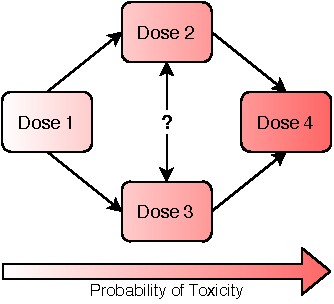
\includegraphics[width=0.75\textwidth]{Adept-DoseExample}
\end{figure}

Wages et al. \cite{wagesContinualReassessmentMethod2011, wagesUsingTimetoeventContinual2013} further developed their work on the PO-CRM to deal with late-onset toxicities by implementing a TITE component. This trial design, referred to as the time-to-event continual reassessment method in the presence of partial orders (PO-TITE-CRM) by the authors, was chosen to be used in ADePT-DDR. A search of PubMed, conducted on the 25th of July 2020, found six articles that had cited the PO-TITE-CRM design by Wages et al. \cite{wagesUsingTimetoeventContinual2013}. Of these six articles non actually implement the design into a trial. The following paragraphs provide more details. 

Five of these papers were methodological in nature, two of which only include the PO-TITE-CRM design in a brief introduction to current methodology before going on to present new Bayesian trial designs \cite{liuBAYESIANDATAAUGMENTATION2013, wheelerBayesianModelfreeApproach2019}. The other three papers were authored by Wages. The first of which details practical considerations and specifications for the PO-CRM design, the TITE variant is only cited as the source of an example which is being used \cite{wagesSpecificationsContinualReassessment2013}. One paper presents an R package 'pocrm' \cite{wagesPocrmRpackagePhase2013, wagesPocrmDoseFinding2019}. The package is only capable of analysing the PO-CRM design. The TITE variant is only referenced here as it illustrates the issue of partial ordering. The last methodological paper by Wages et al. \cite{wagesPracticalDesignsPhase2016} presents three different methods for phase \RN{1} studies of drug combinations one of which is the PO-CRM however, PO-TITE-CRM is only mentioned as an extension to this design. A key message in this paper is the fact that novel methodologies are constantly emerging but are rarely implemented in practice. 

The last paper is a protocol paper for a phase \RN{1}/\RN{2} study, OLA-TMZ-RTE-01 \cite{lesueurPhaseIIaStudy2019}. The phase \RN{1} component of the study aims to determine the recommended phase \RN{2} dose (RP2D) of olaparib combined with a standard schedule of radiotherapy and temozolomide (TMZ) as first line treatment for patients with unresectable glioblastoma (GBM). The treatment schedule is divided into a radiotherapy and maintenance period. They propose to conduct two sequential dose-escalations of seven different  olaparib dose-levels. Patients in the first escalation will be allocated to a dose level of olaparib for 10 weeks including radiotherapy for six weeks with TMZ given each day during radiotherapy and then for six cycles four weeks post radiotherapy during the maintenance period. They state the MTD1 will be determined using a TITE-CRM. Patients in the second escalation olaparib at the MTD1 during the radiotherapy period along with the same schedule of radiotherapy and TMZ. Those patients will then be allocated to one of the seven dose levels of olaparib during the maintenance period. Again, it is stated that the MTD2 will be determined using TITE-CRM modelling. The RP2D is the MTD1 and MTD2 during the radiotherapy and maintenance period respectively. Even though a combination of treatments is being investigated only olaparib is being escalated and doses for other treatments are fixed for all patients. Furthermore, the dose-levels for olaparib increase consistently in either amount or duration meaning there are no issues of partial ordering which would warrant the use of PO-TITE-CRM. The authors reference the TITE-CRM methodology with two papers. One of them being the paper detailing the PO-TITE-CRM design and the other being a paper by Huang and Kuan \cite{huangTimetoeventContinualReassessment2014} which proposes an adaptive weight function that incorporates cyclical data of treatment into the TITE-CRM. It is unclear as to why the PO-TITE-CRM is cited as its methodology is not mentioned anywhere in methods.       

This is just a brief review of the current literature but it seems that the PO-TITE-CRM has rarely been used or discussed since its inception. 

This chapter provides novel insight into the methodology of PO-TITE-CRM through application in a real-world scenario. Section \ref{adept:PO-TITE-CRM-Design} will detail how the PO-TITE-CRM works. Section \ref{adept:PO-TITE-CRM-in-Adept} discusses the justification for implementing the design into the ADePT-DDR trial and our experiences doing so. Section \ref{adept:Exploring-other-designs} explores other alternative designs which could have been implemented and assess how they perform in comparison to the PO-TITE-CRM. We provide some discussion in Section \ref{adept:Discussion} and finally some conclusions in Section \ref{adept:Conclusion}.

%----------------------------------------------------------------------------------------
%	SECTION 2
%----------------------------------------------------------------------------------------
\section{The PO-TITE-CRM Design}
\label{adept:PO-TITE-CRM-Design} 

Wages et al. \cite{wagesUsingTimetoeventContinual2013} introduced the PO-TITE-CRM design which builds directly upon the PO-CRM design by incorporating a TITE component into the dose toxicity model. The aim of which is to determine the target dose for combinations of drugs where the monotonicity assumption does not hold, in a setting where late-onset toxicities are possible.

\begin{table}[h!]
	\centering
	\caption[Example drug combinations with two agents.]{Example of drug combinations for a trial investigating two agents.}
	\label{tab_adept:ex_drug_combo}
	\begin{tabular}{lcccccc}
		\hline  & \multicolumn{6}{c}{\textbf{Drug combinations}}  \\
		\textbf{Agent} & $d_{1}$ & $d_{2}$ & $d_{3}$ & $d_{4}$ & $d_{5}$ & $d_{6}$ \\ \hline
		A (mg/day) & 0.25 & 0.5 & 1.0 & 0.25 & 0.5 & 1.0         \\
		B (mg/day) & 1.0  & 1.0 & 1.0 & 1.5  & 1.5 & 1.5         \\ \hline
	\end{tabular}
\end{table}

To help understand partial ordering, consider an example of an early phase trial investigating the combination of two agents. Drug A which consists of three doses (0.25, 0.5, 1.0 mg/day) and drug B which consists of two doses (1.0, 1.5 mg/day), for a total of six drug combinations $d_{1}$, ..., $d_{6}$ (Table \ref{tab_adept:ex_drug_combo}). For each drug independently we assume they have a monotonic dose-toxicity curve however, the ordering of toxicity probabilities for some of the treatment combinations is unknown. Specifically, we can say $d_{1}$ is less toxic than $d_{2}$ as the dose of drug A increased whilst the dose of drug B stayed the same. This is also the case for $d_{2}$ and $d_{3}$. So, $d_{1}$ can always be considered less toxic than $d_{2}$ which is always less toxic than $d_{3}$. The same can be said for doses $d_{4}$, $d_{5}$ and $d_{6}$, these three doses are can also all be considered more toxic than $d_{1}$ as well.The order between $d_{4}$ and $d_{5}$ in comparison to $d_{3}$ is not known because the dose of drug A decreases whilst the dose of drug B increases. Similarly the order between $d_{2}$ and $d_{4}$ is unknown. Also, we can say that $d_{6}$ is the always the most toxic dose. Assessing all these potential order toxicity relationships leaves five possible orderings. 

\begin{enumerate}
	\centering
	\item $d_{1} \rightarrow d_{2} \rightarrow d_{3} \rightarrow d_{4} \rightarrow d_{5} \rightarrow d_{6}$
	\item $d_{1} \rightarrow d_{2} \rightarrow d_{4} \rightarrow d_{3} \rightarrow d_{5} \rightarrow d_{6}$
	\item $d_{1} \rightarrow d_{2} \rightarrow d_{4} \rightarrow d_{5} \rightarrow d_{3} \rightarrow d_{6}$
	\item $d_{1} \rightarrow d_{4} \rightarrow d_{2} \rightarrow d_{3} \rightarrow d_{5} \rightarrow d_{6}$
	\item $d_{1} \rightarrow d_{4} \rightarrow d_{2} \rightarrow d_{5} \rightarrow d_{3} \rightarrow d_{6}$
\end{enumerate}


Using the notation of Wages et al. \cite{wagesContinualReassessmentMethod2011,wagesUsingTimetoeventContinual2013}, let $M$ denote the number of possible orders and $Y$ be an indicator of a toxicity event. Then for a trial investigating $k$ combinations, $d_{1}$,...,$d_{k}$, the dose for the $j$th patient, $X_{j}$, $j$ = 1,...,$n$ can be thought of as random $x_{j} \in (d_{1}, ..., d_{k})$. For a specific ordering $m$, $m = 1,...,M$ the toxicity probability $R(d_{i})$ is modelled by 
\begin{equation}
R(d_{i}) =  \phi_m(d_i,w,\beta) = w\psi_m(d_i,\beta) \; i = 1, ..., k; \; m = 1, ...,M
\end{equation}
for  a weighted dose response model $\phi_m(d_i,w,\beta)$ where $\beta \in (-\infty, \infty)$. The weight, $w$ as defined by Cheung and Chappel \cite{cheungSequentialDesignsPhase2000}, is a function of the time-to-event of each patient and is incorporated linearly with the dose toxicity model $\psi$ so that $0 \leq w \leq 1$. Each patient is followed for a fixed amount of time $T$. Let $U_j$ represent the time-to-toxicity of patient $j$. Then for $u \leq T$, 
\begin{equation}
	P(U_j \leq u ) = P(U_j \leq u |U_j \leq T)P(U_j \leq T) \equiv w(u;T) \psi_m(d_i,\beta).
\end{equation}
For simplicity we will refer to the weight function $w(u;T)$ as $w$. The weight function will have to be decided upon by the trials team, dependent on the scenario, a simple linear function or a more complex adaptive weights function could be utilised. There are also several working dose models which could be used for $\psi$, Wages et al. \cite{wagesUsingTimetoeventContinual2013} present their design with the power parameter model given by 
\begin{equation}
	\psi_m(d_i,\beta) = \alpha_{mi}^{exp(\beta)} \; i = 1,...,k; \; m = 1,...,M.
\end{equation}
Here $0 < \alpha_{m1} < ... < \alpha_{mk} < 1$ are the prior estimates of toxicity probabilities, or skeleton, for each potential ordering. Furthermore, prior probabilities are assigned to each order $M$ to account for any prior information regarding the plausibility of each model such that, $p(m) = \{p(1),...,p(M)\}$, where $p(m) \geq 0$ and $\sum_mp(m)=1$. When all orders are equally likely or there is no prior information available on possible orderings the prior is discretely uniform and would be $p(m) = 1/M$. 

A Bayesian framework is used and a prior probability distribution $g(\beta)$ is assigned to the parameter $\beta$. The ordering with the largest prior probability is selected as the starting ordering, in the scenario where all priors are equal an ordering is selected at random, subsequently a starting dose is also chosen. After $j$ patients have been entered into the trial data is collected in the form of $\Omega_j = \{x_1,y_1, ..., x_j,y_j\}$. A weighted likelihood for the parameter $\beta$ is used to establish running probabilities of toxicity for each treatment combination. The weighted likelihood under ordering $m$, is given by 
\begin{equation}
\label{eq_adept:likelihood}
\tilde{L}_m(\beta|\Omega_j)=\prod_{l=1}^{j}\phi_m^{y_l}(x_l,w_l,\beta)\{1-\phi_m(x_l,w_l,\beta)\}^{(1-y_l)}
\end{equation} 
which can be used to generate a summary value $\hat{\beta}_{mj}$ for each ordering. With the likelihood and the data $\Omega_j$, the posterior density for $\beta$ can be calculated using 
\begin{equation}
	\tilde{f}_m(\beta|\Omega_j)=\frac{\tilde{L}_m(\beta|\Omega_j)g(\beta)}{\int_{\beta}\tilde{L}_m(\beta|\Omega_j)g(\beta)d\beta}
\end{equation}
This can then be used to establish posterior probabilities of the orderings given the data as 
\begin{equation}
\tilde{\pi}(m|\Omega_j)=\frac{p(m)\int_{\beta}\tilde{L}_m(\beta|\Omega_j)g(\beta)d\beta}{\sum_{m=1}^{M}p(m)\int_{\beta}\tilde{L}_m(\beta|\Omega_j)g(\beta)d\beta}.
\end{equation}
We select the single ordering, $h$, with the largest posterior probability along with its associated working model $\psi_h(d_i,\beta)$ and generate toxicity probabilities for each dose level. Once the $j$th patient has been included the posterior probability of DLT can be calculated for $d_{i}$ so that
\begin{equation}
	\hat{R}(d_i) = \psi_h(d_i,\hat{\beta}_{hj}); \; \hat{\beta}_h = \int_{\beta}\beta\tilde{f}_h(\beta|\Omega_j)d\beta.
\end{equation}

In turn, the dose level $x_j \in \{d_1,...,d_k\}$ assigned to the ($j+$1)th patient is the dose, $d_i$, which minimises 
\begin{equation}
\label{eq_adept:crm_min}
	\triangle(\hat{R}(d_i),\theta) = |\hat{R}(d_i)-\theta|, \; i=1,...,k
\end{equation}
where $\theta$ is the target toxicity rate. Similarly, once all patients have been recruited and observed and the trial ends, the target dose (TD$\theta$) is the dose, $d_{i}$, which minimises (\ref{eq_adept:crm_min}).

%----------------------------------------------------------------------------------------
%	SECTION 3
%-------------------------.

\section{PO-TITE-CRM in ADePT-DDR}  
\label{adept:PO-TITE-CRM-in-Adept}

The decision to implement PO-TITE-CRM into ADePT-DDR was made by Piers Gaunt (PG) after discussions with other statisticians Kristian Brock (KB) and Daniel Slade (DS), as well as the chief investigator and other co-investigators. The design was chosen as the toxicity probabilities of the dose levels weren't monotonically increasing which restricts the use of most early phase designs such as the CRM. Additionally, the design also handles late-onset toxicities which would be an issue in ADePT-DDR due to the treatment involving radiotherapy. The availability of software to conduct the trial was also a factor that was considered. The R package 'pocrm' \cite{wagesPocrmRpackagePhase2013} only provides a means for implementing the PO-CRM design but the easy accessibility to this code meant that it could be extended to include the TITE component.  

The intended use of this design is for dose-finding in combinations of therapies, as this is the source of the partial ordering issue. ADePT-DDR however, is a unique implementation of the design as even though it involves a combination of therapies (radiotherapy and AZD6783) the dose of radiotherapy is fixed and dose-finding is only planned for AZD6783. PO-TITE-CRM is still applicable in this case as the design includes combinations of dose and duration for AZD6783 which are partially ordered. 

A two-stage PO-TITE-CRM will be used to find the TD25 of AZD6783. This will be determined by dose-limiting toxicities evaluated by Common Terminology Criteria for Adverse Events (CTCAE) v5.0 and Radiation Therapy Oncology Group (RTOG) late toxicity score. The binary DLT events are pre-defined by a variety of grade 3-4 adverse events notably, haematological, cardiovascular and gastrointestinal/hepatic toxicities as well as significant non-haematological events and specific treatment-related toxicities. DLTs will be monitored for the duration of treatment (seven weeks) and throughout the follow-up period. The total follow-up period post treatment is 52 weeks, so patients will spend a total of 59 weeks in the trial.  

A maximum of 60 patients will be recruited for the dose-finding aspect of this trial and up to 20 patients as controls. Controls will be utilised to make comparisons for secondary outcomes such as survival and efficacy. Control patients will only be receiving radiotherapy, the dose of which is fixed at 70Gy/35F. Cohorts of three patients will be recruited and assigned to dose levels chosen by the PO-TITE-CRM. Controls will be recruited in the interim period between the recruitment of the third patient in a cohort and the completion of the minimum follow-up period.    

%-----------------------------------
%	SUBSECTION 3.1
%-----------------------------------
\subsection{Partial Ordering in Practice}
\label{adept:Partial-ordering-in-practice}%first number is the chapter number, second number is section number, third is subsection etc..

Each patient entered into ADePT-DDR will receive fixed dose radiation, totalling 70 Gy in 35 fractions over seven weeks. For the dose-finding aspect we investigate six doses of AZD6783 detailed in table \ref{tab_adept:AZD_dose_levels}. Treatment dose and duration to be selected for dose level 3 will be determined based on a combination of data observed, adverse events and compliance. The issue of partial ordering is illustrated in Figure \ref{fig_adept:AZD_dose_levels} inspired from plots by Wages et al. \cite{wagesUsingTimetoeventContinual2013}. The doses to be used in this trial are detailed in their appropriate box. Additionally, each dot represents a potential dose combination which theoretically could be investigated. The combinations are colour coordinated to indicate where partial ordering exists in this dose combination space. Doses across the same colour (each diagonal) cannot be distinguished from each other in terms of probability of toxicity. However, it forms a hierarchy in which doses of the same colour can be thought of as less/more toxic that doses in another colour i.e the red dose levels would have a higher probability of toxicity than the yellow dose levels. It is clear that dose levels 2a and 2b would be considered more toxic than dose level 1 due to the increase in treatment duration and treatment dose respectively. When comparing 2a and 2b it is unknown whether the increase in dose or duration will be more toxic. Hence there are two possible orderings for ADePT-DDR. 

\begin{enumerate}
	\centering
	\item $d_{-1} \rightarrow d_{0} \rightarrow d_{1} \rightarrow d_{2a} \rightarrow d_{2b} \rightarrow d_{3}$
	\item $d_{-1} \rightarrow d_{0} \rightarrow d_{1} \rightarrow d_{2b} \rightarrow d_{2a} \rightarrow d_{3}$
\end{enumerate}

\begin{table}[h!]
    \centering
	\caption[ADePT-DDR dose-levels.]{ADePT-DDR dose-levels and duration of treatment for AZD6783.}
	\label{tab_adept:AZD_dose_levels}
		\begin{tabular}{ccccc}
			\hline 
			\multicolumn{1}{p{1.5cm}}{\centering \textbf{Dose} \\ \textbf{Level}} & \multicolumn{1}{p{3cm}}{\centering \textbf{AZD6783 Daily} \\ \textbf{dose (mg BD)}} &
		    \multicolumn{1}{p{1.5cm}}{\centering \textbf{Weeks} \\ } &
			\multicolumn{1}{p{1.5cm}}{\centering \textbf{Duration} \\ \textbf{(days)}} &
			\multicolumn{1}{p{3.5cm}}{\centering \textbf{Radiotherapy} \\ } 
			\\\hline
			-1 & 20 & 1 & 5 & 70 Gy/ 35 F \\
			 0 & 20 & 1\&4 & 10 & 70 Gy/ 35 F \\
			 1 & 40 & 1\&4 & 10 & 70 Gy/ 35 F \\
			2a & 40 & 1,2,4\&5 & 20 & 70 Gy/ 35 F \\
			2b & 80 & 1\&4 & 10 & 70 Gy/ 35 F \\
			\multirow{2}{*}{3} & 120 & 1\&4 & 10 & 70 Gy/ 35 F \\
			& 80 & 1,2,4\&5 & 20 & 70 Gy/ 35 F \\ \hline
		\end{tabular}
\end{table}

\begin{figure}[h!]
	\centering
	\caption{ADePT-DDR dose levels across dose and duration.}
	\label{fig_adept:AZD_dose_levels}
	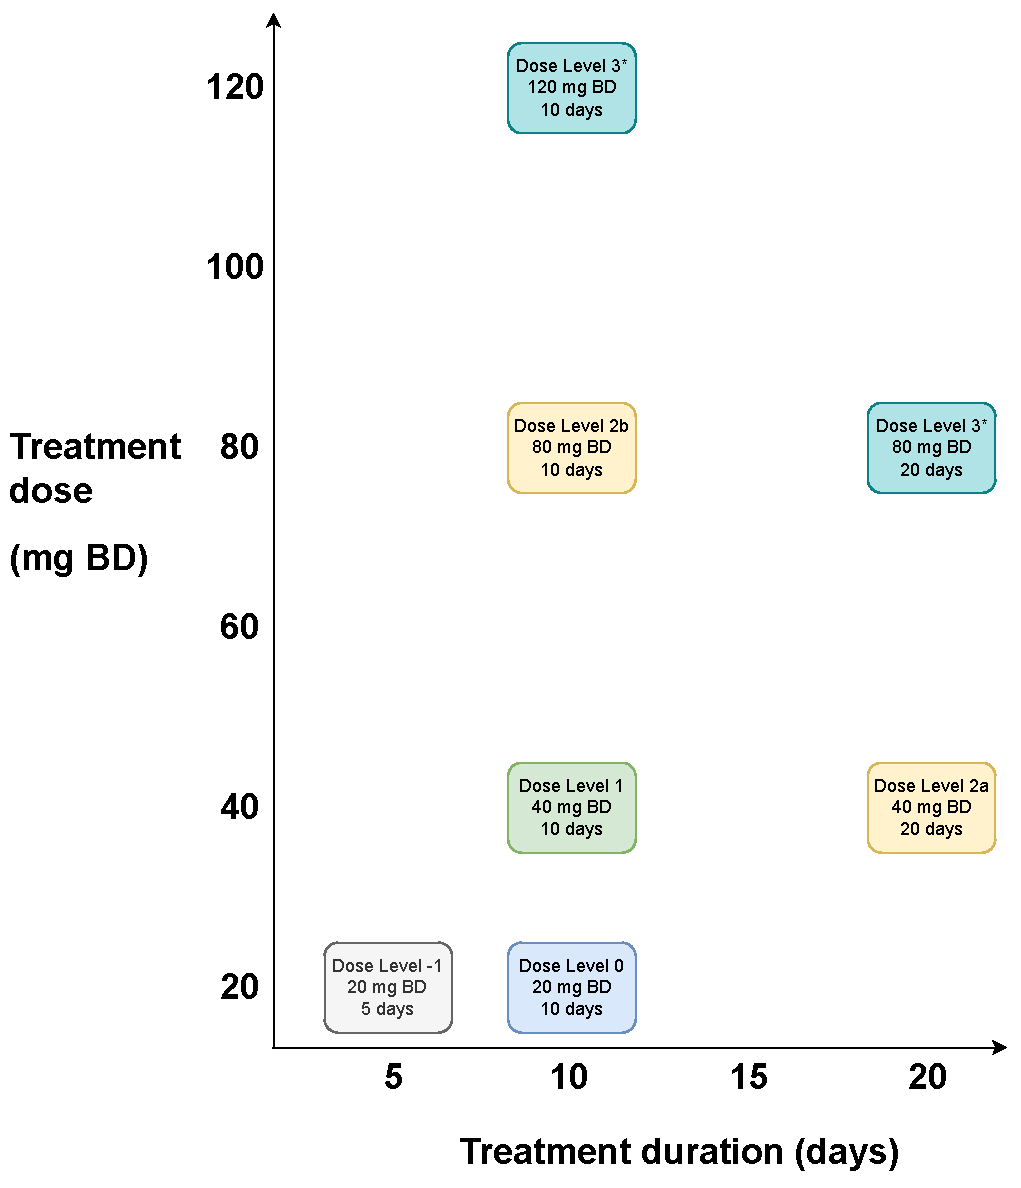
\includegraphics[width=\textwidth]{Adept-DoseCombos}
\end{figure}

Traditionally, dose-finding trials for combinations would select dose levels to form a 'path' through the dose combination space such that each subsequent dose level was logically more toxic. This avoids the issue of partial ordering but means doses of interest or effective dose combinations may be missed or not investigated. Specifically, for ADePT-DDR this allows two 'paths' from dose level 1 extending to 2a and 2b. In terms of dose level 3 only one of the doses in that tier will be investigated, it was unclear as to which dose level would be best due to a lack of historical data. Even though dose level 3 is not yet specified in terms of modelling and simulations it was treated as singular dose. This was done as clinicians thought that it would be unlikely that we'd reach these doses and that the probability of toxicity between them would be similar.  

Preliminary designs of the trial included only five dose levels and planned to use dose level 0 as the starting dose. During the trial design phase it was decided a new lower dose (dose level -1) would be introduced to allow for de-escalation if the initial dose was found to be too toxic. Dose escalation/de-escalation for subsequent cohorts would be determined from the two-stage PO-TITE-CRM. A two-stage design allows for escalation according to a pre-defined escalation scheme similar to a '3+3' design. The first stage dictates that if no DLT's are observed in the current cohort the dose allocated to the next cohort is the following dose in the escalation scheme. Dose levels continue to be incremented in this fashion until the first DLT is observed. In stage two, dose levels are determined by the PO-TITE-CRM.

Typically CRM designs begin by testing the first patient, or cohort, at the prior guess of TD or at a lower dose to be safe. However, clinicians may have safety concerns beginning the trial at higher dose levels as well as escalating to higher dose levels without testing lower ones. Investigators in ADePT-DDR expressed similar concerns as such a two-stage design was adopted. The escalation scheme used in stage one of ADePT-DDR will follow that of the first ordering ($d_{-1} \rightarrow d_{0} \rightarrow d_{1} \rightarrow d_{2a} \rightarrow d_{2b} \rightarrow d_{3}$). If patients in the first cohort (assigned to dose level 0) don't experience a DLT the next cohort will be allocated to dose level 1 and then if no DLTs are observed again the third cohort will be allocated to dose level 2a and so on and so forth. The dose escalation scheme was determined based on the prior probabilities of toxicity generated for each dose level.  

Information elicited from the investigators helped generate prior probabilities of toxicity for each dose level. They believed that dose level 2b would be the TD25 with 2a being less toxic. This was used in conjunction with the getprior function from the dfcrm R package \cite{cheungDfcrmDoseFindingContinual2019} which yielded priors of 0.012, 0.036, 0.084, 0.157, 0.25 and 0.355 for dose levels -1, 0, 1, 2a, 2b and 3 respectively. The half-width of the indifference interval was set at 0.05. The indifference interval is an interval in which the toxicity probability of the selected dose will eventually fall. Prior probabilities are also required for the plausibility of each model and even though the clinicians think that 2b will be more toxic than 2a there is no clear evidence and still a lot of uncertainty. As such it is sensible to assume a plausibility probability of 0.5 for each ordering, implying both orders are equally likely to be the true ordering of these dose levels. 

%-----------------------------------
%	SUBSECTION 3.2
%-----------------------------------
\subsection{The TITE component}
\label{adept:The-TITE-component}

The observation window for this trial will be up to a year post-treatment as the combination of radiotherapy with AZD6738 is anticipated to cause late-onset toxicity. The Acute DLT observation period is 12 weeks (84 days) post radiotherapy end with a minimum of 8 weeks (56 days) for the last patient of each cohort. However, patients will continuously be monitored for occurrence of DLT for at least12 weeks (84 days), i.e. at least 12 weeks (84 days) from the end of radiotherapy. The full window will last for 52 weeks (365 days) post-treatment.

The TITE component incorporates a weighting contribution for each patient dependent on how long that patient has been evaluable in the study. This allows a patient to be evaluated once they have been observed for the minimum DLT period of 8 weeks (56 days). The weighting at this point is 60\% rising to 80\% at 12 weeks (84 days). A patient will not contribute fully to the model until they have completed 52 weeks (365 days) follow up (or have experienced a DLT at any stage in which case they will be weighted as a whole contribution). Linear weighting functions will be employed for any patient with a length of follow up between these three time points. One weight function to calculate weights between 8-12 weeks and another for weights between 12-52 weeks. For the weighting function $w(u;t_1, t_2, t_3)$ where $u$ is the time-to-toxicity of patient $j$ and $t_1, t_2, t_3$ is the time period with values 8, 12 and 52 respectively. Then for $t_1 \leq u \leq t_3$
\begin{equation}
w(u;t_1,t_2,t_3) = 0.6 + 0.2\frac{min(0, min(u, t_2) - t_1)}{t_2 - t_1} + 0.2\frac{max(0, u - t_2)}{t_3-t_2}.
\end{equation} 
All patients will have a minimum weight of 60\% as that is the prescribed weighting to the  minimum follow up period before dose escalation/de-escalation decisions can be made. For each additional week the patient is observed, without a DLT occurring, between weeks 8 and 12 their weighting increases by 5\%. Similarly for each week between 12 and 52 weeks, without a DLT, weighting increases by 0.5\%. Figure \ref{fig_adept:weight_function} illustrates the weight function and how the weight changes for patients dependent on how long they have been followed-up.   

\begin{figure}[h!]
	\centering
	\caption[Weight function across the follow-up period.]{Weights of patients who have not experienced a DLT across the observation window.}
	\label{fig_adept:weight_function}
	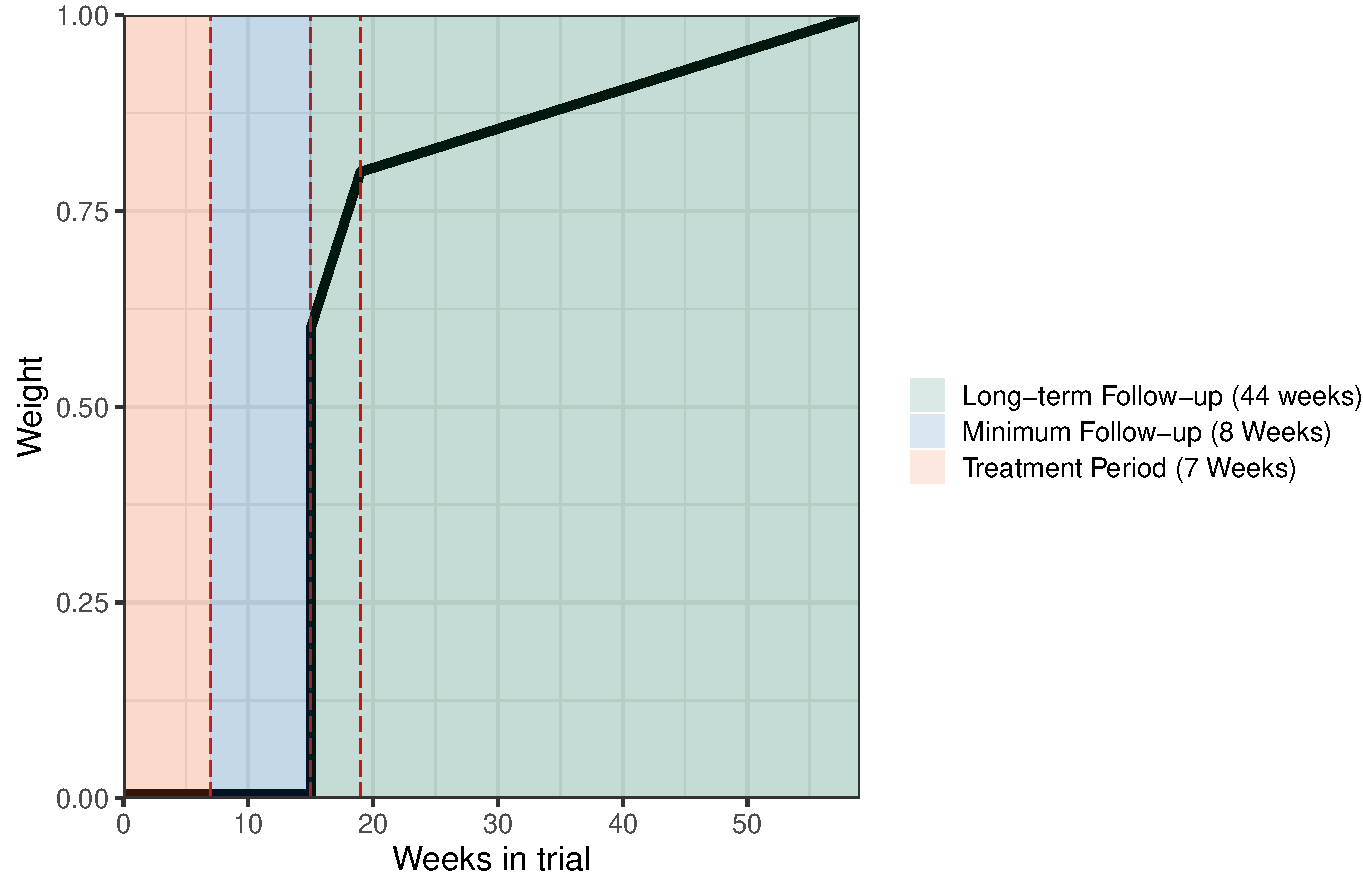
\includegraphics[width=\textwidth]{Adept-WeightFunction}
\end{figure}


The TITE-CRM originally presented by Cheung and Chappel \cite{cheungSequentialDesignsPhase2000} did not incorporate a minimum follow-up period and their design allowed for the continual recruitment of patients whenever they became available. There are some practical considerations which make this infeasible in ADePT-DDR. The model would need to be run each time a new patient entered the study which requires statistical input hence the introduction of cohorts. Clinicians may also have safety concerns if we see rapid recruitment at the start of the trial and the model keeps escalating so we impose a minimum follow-up period. Initially this was set at 12 weeks (at 80\% weighting) however, statisticians AP and PG  pointed out that dose escalation/de-escalation decisions would have to take place 19 weeks (7 weeks treatment and 12 weeks follow-up) after recruitment of the third patient in the cohort. Dependent on the recruitment rates this could extend the duration of the trial and negates the benefits of using a TITE design. The investigators aslo agreed this was too long and settled on lowering this period to 8 weeks (at 60\% weighting) whilst also including the original 12 week weighting of 80\%.


%-----------------------------------
%	SUBSECTION 3.3
%-----------------------------------
\subsection{Stopping Rules}
\label{adept:Stopping-rules}

A practical modification was included to allow for early stopping of the trial if there is sufficient evidence that the TD has been reached. Sufficient evidence is achieved once 15 patients (five cohorts) have been treated at the same dose level and the model allocates that dose level again to a sixth cohort. This rule evolved from the original designs of the trial which involved 30 patients with a dose expansion cohort to ensure at least 15 patients were treated at the TD. 

Initial simulations highlighted the inadequacy of these design parameters as operating characteristics for various scenarios were poor, specifically in terms of correct TD selection. Clinicians explained the inclusion of the dose expansion cohort was to ensure the dose-finding aspect of the trial did not take a large amount of time whilst also allowing safety to be assessed at the TD. In order to ensure that a reasonable amount of patients would be treated at the TD, the trial wouldn't take longer than necessary and operating characteristics improved, the sample size was increase and this rule was introduced.

A rule was also implemented to allow for early termination of the trial in the case of excess toxicity at the lowest dose. If the probability of DLT at the lowest dose is higher than 0.35 with a probability of 80\% and has been tested the trials safety committee will be alerted and will recommend if the trial should be stopped. As the trial starts at dose level 0, which is not the lowest dose, it is possible for the trial to recommend terminating without ever allocating patients to the lowest dose level. As such it was decided early termination would only occur once at least 3 patients (1 cohort) have been allocated dose level -1. 

An approximate estimate of the variance was calculated using methodology presented by O'Quigley and Shen \cite{oquigleyContinualReassessmentMethod1996}. The observed information matrix is obtained by taking the second derivative of the likelihood (eq. \ref{eq_adept:likelihood}) which is then used to calculate the variance $v(\hat{\beta_j})$, for estimate $\beta_j$ which becomes more accurate with larger sample sizes. After each cohort, we sample many times from a normal distribution with parameters based on the estimate of $\beta_j$ and its variance. These samples are then plugged into our dose-toxicity model to ascertain the probability of toxicity at the lowest dose. The trial will be recommended to stop if it breaks the rule based on the criteria above. 


%-----------------------------------
%	SUBSECTION 3.4 
%-----------------------------------
\subsection{Operating Characteristics}
\label{adept:OCs} 

Simulations were continually utilised during the design process of the trial to assess how various changes impact the overall performance. These changes to design features such as the sample size, weight function and stopping rules helped inform decisions which led to the final design.  

Functions from pocrm package in R \cite{wagesPocrmRpackagePhase2013, wagesPocrmDoseFinding2019} were modified in order to perform simulations and conduct the trial. The majority of work involved integrating the TITE component and the stopping rules into the code. In standard CRM designs a binary outcome for toxicity is generated for each patient based on a pre-specified true DLT rates for the dose they are assigned. Adding the TITE component means the time the toxicity occurs also has to be generated, the simulation must also track this time and incorporate this information into the PO-TITE-CRM model when it needs to make dose allocation decisions for the next cohort. We defined multiple scenarios to reflect various real life possibilities in order to assess the designs performance.  

Standard scenarios to run involve adjusting the true DLT rates to reflect each dose being the TD25. For each of these we calculate the probability of selecting each dose as the TD25. It would be expected the dose with the highest probability of being selected has its true DLT rate set at 25\% to match the target rate. A high probability of selection for the correct dose implies the design works well in the specified scenario. Additional characteristics such as the average number of patients at each dose level are also investigated. This can be used to look at how many patients may potentially be allocated to a toxic dose. It is also necessary to consider performance when all doses are too toxic, here we would want the design to recommend stopping early. Usually the true DLT rates used to define these scenarios abide by the monotonicity assumption. Due to the partial ordering we consider scenarios in which the true DLT rates follow both orders. For trials with a large amount of orders it may be unfeasible to run so many simulations. However, as ADePT-DDR only has two orders we explored all scenarios for each ordering.

We simulated 10000 trials for each scenario using the finalised design detailed in section \ref{adept:PO-TITE-CRM-in-Adept}. Simulations were based on the assumption that the trial would recruit one patient per month. The occurrence of DLT's were randomly generated for patients in each cohort using a Bernoulli distribution with the probability set at the true DLT rate for the cohorts assigned dose level in the specific scenario. For patients who had a DLT occur, the time at which the DLT occurred was randomly generated using a uniform distribution which spanned the start of treatment to the end of follow-up. The simulations presented in Tables \ref{tab_adept:OCorder1} and \ref{tab_adept:OCorder2} took approximately 5 hours and 53 minutes to run. The Monte Carlo standard error for probabilities estimated by 10000 simulations is $\sqrt{0.5 \times 0.5/10000} = 0.5\%$.

Table \ref{tab_adept:OCorder1} details simulations for eight scenarios to test the performance of the PO-TITE-CRM design using true DLT rates which reflect the first ordering. We analyse scenarios where each dose is the TD25 (scenarios 1-6) and when all doses are too toxic (scenario 8). Additionally, we also investigate performance under conditions where the probability of DLT is fairly similar between doses (scenario 7). This is a notoriously difficult circumstance for CRM designs to deal with as the limited number of patients and events at each dose make it hard to accurately estimate toxicity probabilities if they are similar. Simulation results for ordering 2 are shown in Table \ref{tab_adept:OCorder2} where dose level 2a is considered more toxic than 2b. This is achieved by altering the true DLT rates so 2b has a lower probability of DLT compared to 2a. 

Ideally we want the probability of selection for the dose allocated at TD25 to be as high as possible and greater than other dose levels. For scenarios 1-7 the TD25 is highlighted in bold along with results from the simulations. However, for scenario 8 where all doses are too toxic we expect the trial to terminate early, here 'stop' should be selected and its associated probability of stopping is shown in bold. 

\begin{table}[h!] % OC for order 1 
	
	\caption[Operating Characteristics for ordering 1.]{\label{tab_adept:OCorder1} Operating Characteristics of the two-stage PO-TITE-CRM (with true DLT rates that imply 2b is more toxic than 2a) based on 10000 simulated trials. Definitions: DLT: Dose-limiting toxicity. P(select):
		Probability of selecting a dose as the TD25.}
	\centering
	\begin{singlespace}
		\resizebox{\linewidth}{!}{
			\begin{tabular}[t]{ccccccccc}
				\toprule
				\multicolumn{2}{c}{ } & \multicolumn{6}{c}{Dose Levels} \\
				\cmidrule(l{3pt}r{3pt}){3-8}
				&  & -1 & 0 & 1 & 2a & 2b & 3 & Stop\\
				\midrule
				Scenario & Prior DLT & 0.01 & 0.04 & 0.08 & 0.16 & 0.25 & 0.35 & \\
				\cmidrule{1-9}
				\rowcolor{gray!6}   & True DLT rate & 0.25 & 0.4 & 0.45 & 0.5 & 0.55 & 0.6 & \\
				
				\rowcolor{gray!6}   & P(select) & 0.68 & 0.18 & 0.05 & 0.01 & 0 & 0 & 0.0849\\
				
				\rowcolor{gray!6}   & \% of patients & 39 & 32 & 20 & 6 & 3 & 0 & \\
				
				\rowcolor{gray!6}  \multirow{-4}{*}{\centering\arraybackslash 1: TD25 @-1} & Mean number of patients & 10.17 & 8.46 & 5.33 & 1.67 & 0.69 & 0.07 & \\
				\cmidrule{1-9}
				& True DLT rate & 0.12 & 0.25 & 0.4 & 0.45 & 0.5 & 0.55 & \\
				
				& P(select) & 0.23 & 0.51 & 0.2 & 0.03 & 0.02 & 0 & 0.0079\\
				
				& \% of patients & 17 & 35 & 29 & 11 & 6 & 1 & \\
				
				\multirow{-4}{*}{\centering\arraybackslash 2: TD25 @0} & Mean number of patients & 5.24 & 10.48 & 8.75 & 3.4 & 1.83 & 0.26 & \\
				\cmidrule{1-9}
				\rowcolor{gray!6}   & True DLT rate & 0.09 & 0.12 & 0.25 & 0.4 & 0.45 & 0.5 & \\
				
				\rowcolor{gray!6}   & P(select) & 0.02 & 0.2 & 0.55 & 0.14 & 0.09 & 0.01 & 4e-04\\
				
				\rowcolor{gray!6}   & \% of patients & 4 & 20 & 34 & 23 & 16 & 3 & \\
				
				\rowcolor{gray!6}  \multirow{-4}{*}{\centering\arraybackslash 3: TD25 @1} & Mean number of patients & 1.22 & 6.41 & 10.97 & 7.23 & 5.14 & 1.02 & \\
				\cmidrule{1-9}
				& True DLT rate & 0.06 & 0.09 & 0.12 & 0.25 & 0.4 & 0.45 & \\
				
				& P(select) & 0 & 0.02 & 0.22 & 0.48 & 0.23 & 0.05 & 1e-04\\
				
				& \% of patients & 1 & 12 & 20 & 31 & 25 & 11 & \\
				
				\multirow{-4}{*}{\centering\arraybackslash 4: TD25 @2a} & Mean number of patients & 0.47 & 3.88 & 6.74 & 10.43 & 8.2 & 3.5 & \\
				\cmidrule{1-9}
				\rowcolor{gray!6}   & True DLT rate & 0.03 & 0.06 & 0.09 & 0.12 & 0.25 & 0.4 & \\
				
				\rowcolor{gray!6}   & P(select) & 0 & 0 & 0.02 & 0.3 & 0.43 & 0.25 & 0\\
				
				\rowcolor{gray!6}   & \% of patients & 1 & 10 & 12 & 24 & 28 & 25 & \\
				
				\rowcolor{gray!6}  \multirow{-4}{*}{\centering\arraybackslash 5: TD25 @2b} & Mean number of patients & 0.25 & 3.36 & 4.15 & 8.17 & 9.33 & 8.33 & \\
				\cmidrule{1-9}
				& True DLT rate & 0.01 & 0.03 & 0.06 & 0.09 & 0.12 & 0.25 & \\
				
				& P(select) & 0 & 0 & 0 & 0.09 & 0.13 & 0.78 & 0\\
				
				& \% of patients & 0 & 10 & 11 & 18 & 18 & 42 & \\
				
				\multirow{-4}{*}{\centering\arraybackslash 6: TD25 @3} & Mean number of patients & 0.1 & 3.13 & 3.49 & 5.46 & 5.6 & 13.14 & \\
				\cmidrule{1-9}
				\rowcolor{gray!6}   & True DLT rate & 0.05 & 0.1 & 0.15 & 0.2 & 0.25 & 0.3 & \\
				
				\rowcolor{gray!6}   & P(select) & 0 & 0.03 & 0.12 & 0.31 & 0.28 & 0.26 & 3e-04\\
				
				\rowcolor{gray!6}   & \% of patients & 2 & 13 & 18 & 26 & 23 & 19 & \\
				
				\rowcolor{gray!6}  \multirow{-4}{*}{\centering\arraybackslash 7: Equal steps in DLT rate} & Mean number of patients & 0.55 & 4.03 & 5.72 & 8.32 & 7.15 & 5.96 & \\
				\cmidrule{1-9}
				& True DLT rate & 0.5 & 0.6 & 0.65 & 0.7 & 0.75 & 0.8 & \\
				
				& P(select) & 0.26 & 0 & 0 & 0 & 0 & 0 & 0.7404\\
				
				& \% of patients & 56 & 26 & 15 & 2 & 0 & 0 & \\
				
				\multirow{-4}{*}{\centering\arraybackslash 8: All  toxic} & Mean number of patients & 9.05 & 4.27 & 2.4 & 0.37 & 0.04 & 0 & \\
				\bottomrule
			\end{tabular}
		}
	\end{singlespace}
\end{table}

\begin{table}[h!] % OC for order 2
	
	\caption[Operating Characteristics for ordering 2.]{\label{tab_adept:OCorder2}  Operating Characteristics of the two-stage PO-TITE-CRM (with true DLT rates that imply 2a is more toxic than 2b) based on 10000 simulated trials. Definitions: DLT: Dose-limiting toxicity. P(select): Probability of selecting a dose as the TD25.}
	\centering
	\begin{singlespace}
		\resizebox{\linewidth}{!}{
			\begin{tabular}[t]{ccccccccc}
				\toprule
				\multicolumn{2}{c}{ } & \multicolumn{6}{c}{Dose Levels} \\
				\cmidrule(l{3pt}r{3pt}){3-8}
				&  & -1 & 0 & 1 & 2a & 2b & 3 & Stop\\
				\midrule
				Scenario & Prior DLT & 0.01 & 0.04 & 0.08 & 0.16 & 0.25 & 0.35 & \\
				\cmidrule{1-9}
				\rowcolor{gray!6}   & True DLT rate & 0.25 & 0.4 & 0.45 & 0.55 & 0.5 & 0.6 & \\
				
				\rowcolor{gray!6}   & P(select) & 0.67 & 0.19 & 0.05 & 0 & 0.01 & 0 & 0.0827\\
				
				\rowcolor{gray!6}   & \% of patients & 39 & 32 & 20 & 6 & 3 & 0 & \\
				
				\rowcolor{gray!6}  \multirow{-4}{*}{\centering\arraybackslash 9: TD25 @-1} & Mean number of patients & 10.19 & 8.43 & 5.27 & 1.6 & 0.68 & 0.07 & \\
				\cmidrule{1-9}
				& True DLT rate & 0.12 & 0.25 & 0.4 & 0.5 & 0.45 & 0.55 & \\
				
				& P(select) & 0.23 & 0.52 & 0.2 & 0.02 & 0.02 & 0 & 0.0074\\
				
				& \% of patients & 18 & 36 & 29 & 11 & 6 & 1 & \\
				
				\multirow{-4}{*}{\centering\arraybackslash 10: TD25 @0} & Mean number of patients & 5.24 & 10.64 & 8.82 & 3.16 & 1.85 & 0.24 & \\
				\cmidrule{1-9}
				\rowcolor{gray!6}   & True DLT rate & 0.09 & 0.12 & 0.25 & 0.45 & 0.4 & 0.5 & \\
				
				\rowcolor{gray!6}   & P(select) & 0.02 & 0.2 & 0.55 & 0.09 & 0.14 & 0.01 & 4e-04\\
				
				\rowcolor{gray!6}   & \% of patients & 4 & 20 & 34 & 21 & 17 & 3 & \\
				
				\rowcolor{gray!6}  \multirow{-4}{*}{\centering\arraybackslash 11: TD25 @1} & Mean number of patients & 1.16 & 6.43 & 11.07 & 6.83 & 5.6 & 1.07 & \\
				\cmidrule{1-9}
				& True DLT rate & 0.06 & 0.09 & 0.12 & 0.25 & 0.15 & 0.45 & \\
				
				& P(select) & 0 & 0.01 & 0.08 & 0.44 & 0.33 & 0.14 & 2e-04\\
				
				& \% of patients & 1 & 11 & 16 & 30 & 24 & 18 & \\
				
				\multirow{-4}{*}{\centering\arraybackslash 12: TD25 @2a} & Mean number of patients & 0.48 & 3.78 & 5.24 & 10.1 & 7.9 & 6.07 & \\
				\cmidrule{1-9}
				\rowcolor{gray!6}   & True DLT rate & 0.03 & 0.06 & 0.09 & 0.35 & 0.25 & 0.4 & \\
				
				\rowcolor{gray!6}   & P(select) & 0 & 0 & 0.15 & 0.31 & 0.43 & 0.11 & 0\\
				
				\rowcolor{gray!6}   & \% of patients & 1 & 11 & 18 & 30 & 28 & 14 & \\
				
				\rowcolor{gray!6}  \multirow{-4}{*}{\centering\arraybackslash 13: TD25 @2b} & Mean number of patients & 0.25 & 3.5 & 5.9 & 9.82 & 9.14 & 4.54 & \\
				\cmidrule{1-9}
				& True DLT rate & 0.01 & 0.03 & 0.06 & 0.12 & 0.09 & 0.25 & \\
				
				& P(select) & 0 & 0 & 0 & 0.13 & 0.09 & 0.78 & 0\\
				
				& \% of patients & 0 & 10 & 11 & 19 & 16 & 43 & \\
				
				\multirow{-4}{*}{\centering\arraybackslash 14: TD25 @3} & Mean number of patients & 0.1 & 3.13 & 3.51 & 5.88 & 5.06 & 13.13 & \\
				\cmidrule{1-9}
				\rowcolor{gray!6}   & True DLT rate & 0.05 & 0.1 & 0.15 & 0.25 & 0.2 & 0.3 & \\
				
				\rowcolor{gray!6}   & P(select) & 0 & 0.02 & 0.12 & 0.32 & 0.27 & 0.26 & 2e-04\\
				
				\rowcolor{gray!6}   & \% of patients & 2 & 13 & 19 & 27 & 22 & 18 & \\
				
				\rowcolor{gray!6}  \multirow{-4}{*}{\centering\arraybackslash 15: Equal steps in DLT rate} & Mean number of patients & 0.54 & 4.02 & 5.93 & 8.56 & 6.89 & 5.75 & \\
				\cmidrule{1-9}
				& True DLT rate & 0.5 & 0.6 & 0.65 & 0.75 & 0.7 & 0.8 & \\
				
				& P(select) & 0.27 & 0 & 0 & 0 & 0 & 0 & 0.7273\\
				
				& \% of patients & 56 & 27 & 15 & 2 & 0 & 0 & \\
				
				\multirow{-4}{*}{\centering\arraybackslash 16: All  toxic} & Mean number of patients & 9.01 & 4.28 & 2.39 & 0.38 & 0.05 & 0 & \\
				\bottomrule
		\end{tabular}}
	\end{singlespace}
\end{table}

In scenarios 1 - 6 (Table \ref{tab_adept:OCorder1}), this design correctly selects the TD25 with probabilities between 43\% and 78\%, under the assumption 2b is more toxic than 2a. Likewise, for the ordering where 2a is more toxic than 2b, scenarios 9-14 (Table \ref{tab_adept:OCorder2}) have probabilities between 43\% and 78\% of correctly selecting the TD25. Correct selection probabilities are generally higher when the TD25 is at the first and last dose levels compared to dose levels 2a and 2b. However, these dose levels are still chosen with the highest probability as the TD25 in their given scenarios. For scenarios 7 and 15, the probabilities of toxicity are equally spaced, approximately 5\% apart. This is a relatively diffcult scenario for dose-finding studies to handle. The probability of selecting the TD25 is 28\% and 32\% for orderings 1 and 2 respectively and even if the performance is poor the correct dose is still likely to be selected. In scenarios 8 and 16, where all the doses are too toxic, the design very seldom allocates patients higher than the first three doses and there is a high chance (74\% and 73\% respectively) that the trial will recommend early stopping.

Additionally, we assess designs based on how doses are allocated to patients. Designs may correctly select the TD however, this could be undesirable and unethical if the majority of patients are over dosed at the more toxic dose levels. The average number and the percentage of patients at each dose level, for each scenario, is recorded in Tables \ref{tab_adept:OCorder1} and \ref{tab_adept:OCorder2}. 

The percentage of patients treated at the TD25 ranges between 23\% and 43\% for each scenario under both orderings. The design also allocates the most patients on average to the TD25 apart from in scenario 7. In this case more patients were allocated to the next lowest dose, we have already discussed the difficulties of this scenario so this characteristic is not too concerning. The mean number of patients recruited for scenarios 1-6 is 26, 30, 32, 33, 34 and 31 respectively. Similarly for scenarios 9-14 its 26, 30, 32, 34, 33 and 31. Even though we allow for up to 60 patients the majority of trials terminate early based on the pre-defined rules for selecting the TD25. This information is presented in Table \ref{tab_adept:SummaryN_POTITESims} which also shows how often the max sample size is reached from the 10000 trials for each scenario. 

\begin{table}[h!]
	
	\caption{\label{tab_adept:SummaryN_POTITESims}Summary of simulated patient numbers for each scenario.}
	\centering
	\resizebox{\linewidth}{!}{
		\begin{tabular}[t]{cccc}
			\toprule
				Scenario & Max no. of patients & \% max reached & Mean no. of patients\\
				\midrule
				\cellcolor{gray!6}{1: TD25 @-1} & \cellcolor{gray!6}{60} & \cellcolor{gray!6}{0.21} & \cellcolor{gray!6}{26.38}\\
				2: TD25 @0 & 60 & 0.08 & 29.97\\
				\cellcolor{gray!6}{3: TD25 @1} & \cellcolor{gray!6}{60} & \cellcolor{gray!6}{0.05} & \cellcolor{gray!6}{32.01}\\
				4: TD25 @2a & 60 & 0.12 & 33.22\\
				\cellcolor{gray!6}{5: TD25 @2b} & \cellcolor{gray!6}{60} & \cellcolor{gray!6}{0.06} & \cellcolor{gray!6}{33.60}\\
				6: TD25 @3 & 60 & 0.02 & 30.92\\
				\cellcolor{gray!6}{7: Equal steps} & \cellcolor{gray!6}{60} & \cellcolor{gray!6}{0.01} & \cellcolor{gray!6}{31.74}\\
				8: All toxic & 54 & 0.01 & 16.14\\
				\cellcolor{gray!6}{9: TD25 @-1} & \cellcolor{gray!6}{60} & \cellcolor{gray!6}{0.17} & \cellcolor{gray!6}{26.24}\\
				10: TD25 @0 & 60 & 0.11 & 29.95\\
				\cellcolor{gray!6}{11: TD25 @1} & \cellcolor{gray!6}{60} & \cellcolor{gray!6}{0.06} & \cellcolor{gray!6}{32.15}\\
				12: TD25 @2a & 60 & 0.07 & 33.56\\
				\cellcolor{gray!6}{13: TD25 @2b} & \cellcolor{gray!6}{60} & \cellcolor{gray!6}{0.03} & \cellcolor{gray!6}{33.16}\\
				14: TD25 @3 & 60 & 0.08 & 30.81\\
				\cellcolor{gray!6}{15: Equal steps} & \cellcolor{gray!6}{60} & \cellcolor{gray!6}{0.02} & \cellcolor{gray!6}{31.69}\\
				16: All toxic & 51 & 0.01 & 16.11\\
			\bottomrule
	\end{tabular}}
\end{table}




Overall, the simulation results show the specification of this design performs relatively well in a number of scenarios. We have shown there is a high probability of the trial stopping early if all dose-levels are too toxic. We have also shown the design behaves in an appropriate manner when there is a lack of disparity between dose-levels in terms of toxicity. Finally, we have demonstrated that regardless of the ordering we observe the PO-TITE-CRM has a high probability of selecting the correct dose. There are a number of limitations to the operating characteristics presented here which are due to the specification of the simulations and trial design. Section \ref{adept:Exploring-other-designs} explores and discusses these limitations in more detail.

%----------------------------------------------------------------------------------------
%	SECTION 4
%-------------------------.

\section{Exploring other designs}  
\label{adept:Exploring-other-designs}

The operating characteristics presented in section \ref{adept:OCs} provide an insight into how the trial design operates and its effectiveness at selecting the TD25. However, several factors impact the results seen here. These factors can be grouped into two main categories, limitations with the simulations performed or the trial design.

To simulate various scenarios the true DLT rates are adjusted to reflect the TD25 being at different dose levels. There is no formal process to select these values as such their selection is fairly arbitrary. We set one dose level as the TD25 with lower and higher dose levels set at lower and higher DLT rates respectively. Figure \ref{fig_adept:dlt_rates} illustrates the dose levels for scenarios in Table \ref{tab_adept:OCorder1} where dose level 2b is more toxic than 2a. The DLT rates cover some possible scenarios and account for a range of plausible values. However, these true DLT rates may not accurately reflect what we observe once the trial begins. Also, the relationship between the rates and the dose levels may not be similar to what we use in the simulations. Multiple other scenarios could be investigated but it would still be impossible to account for all possible variations which may occur. Hence when evaluating the performance of a design it is important to note the scenario in which it is being evaluated and whether or not the design performs as expected and to an adequate level. For ADePT-DDR, the design produces reasonable operating characteristics under each scenario. 

\begin{figure}[h!]
	\centering
	\caption[Illustration of true DLT rates used in simulations.]{True DLT rates used for each of the scenarios where dose level 2b is more toxic than 2a. The dotted red line represents the target dlt rate of 25\% (TD25).}
	\label{fig_adept:dlt_rates}
	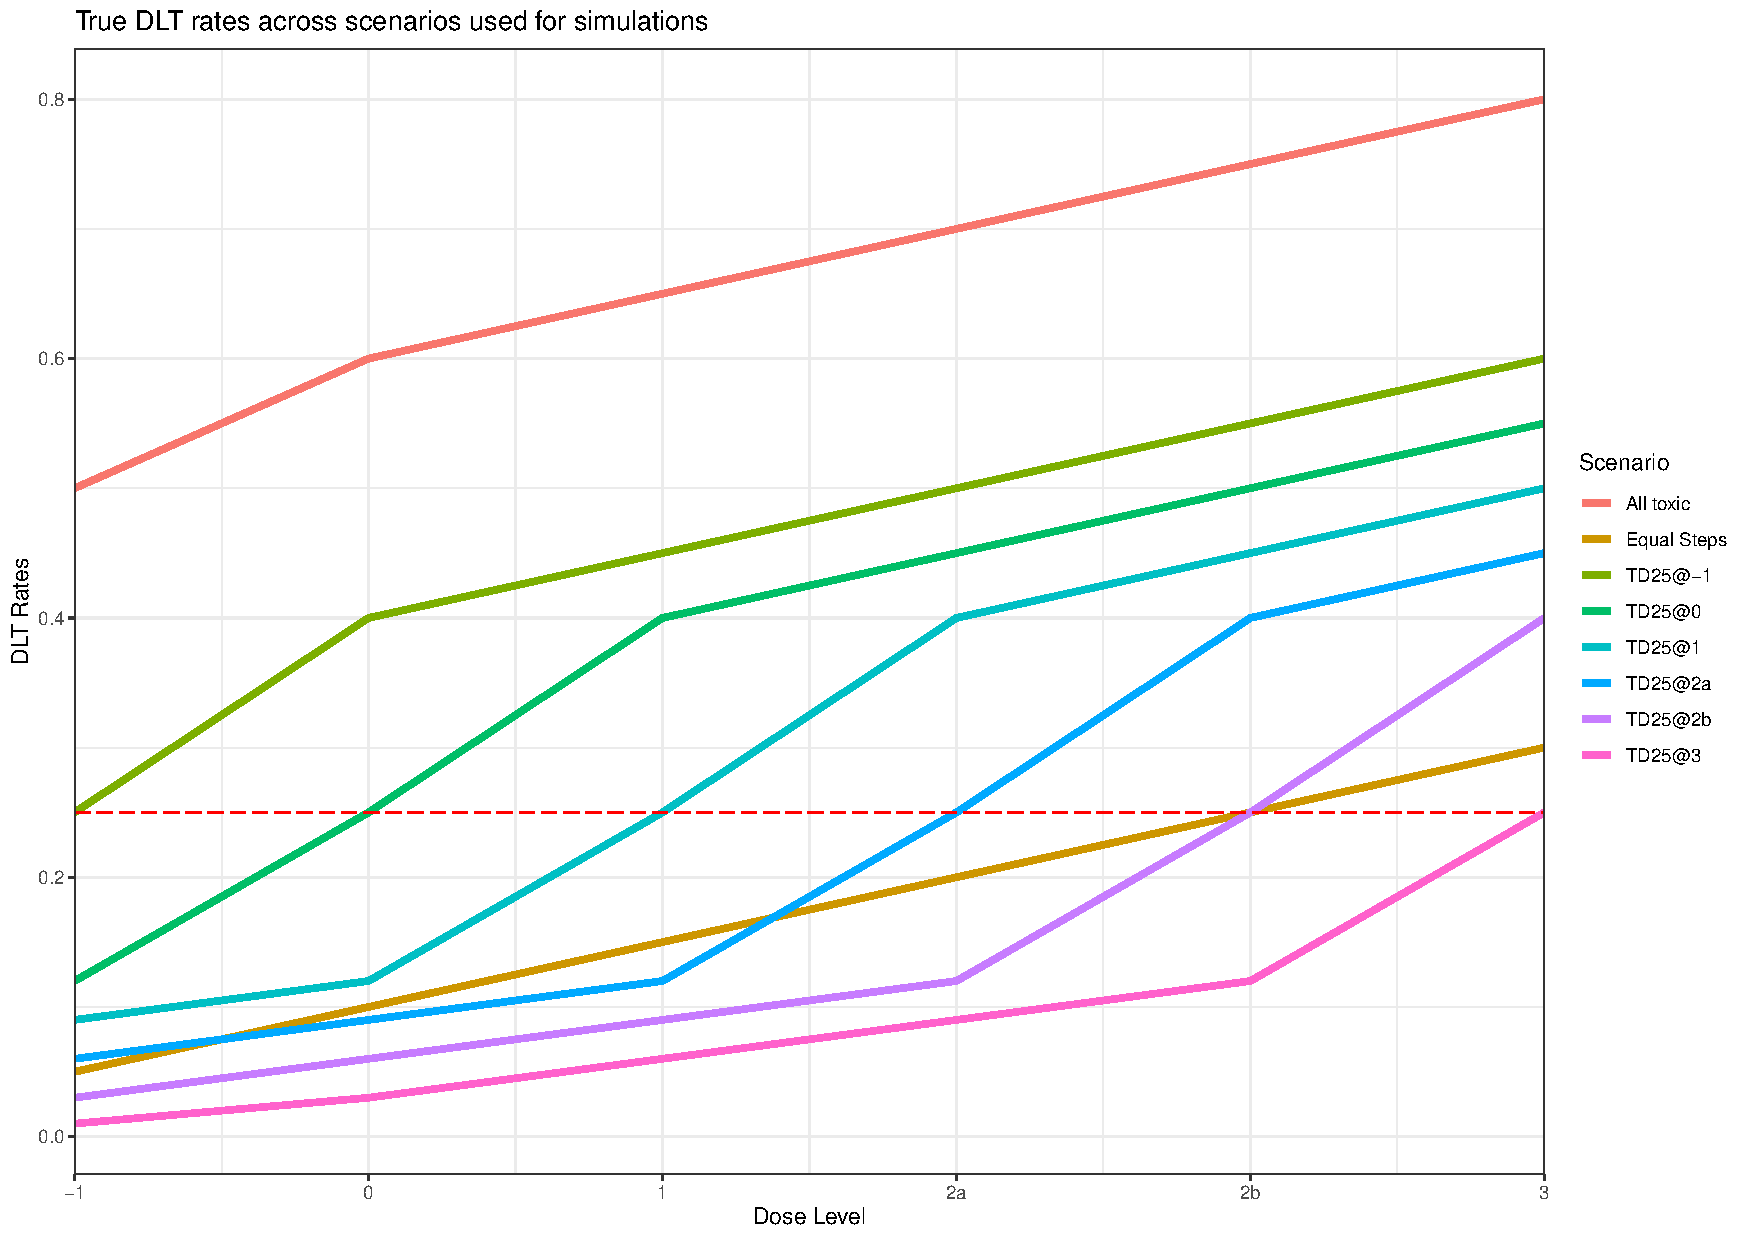
\includegraphics[width=\textwidth]{Adept-DLTRates}
\end{figure}
 
The original methodological papers by Wages et al. \cite{wagesUsingTimetoeventContinual2013,wagesContinualReassessmentMethod2011} only provide simulations for their examples using true DLT rates that are monotonically increasing which represented one of their possible orderings. We cannot tell how their design would perform under scenarios from different orderings. It is unclear as to why this wasn't examined. Initially, in ADePT-DDR we followed suit and only produced simulations under a monotonically increasing DLT rate (order where 2b is more toxic than 2a, Table \ref{tab_adept:OCorder1}). However, as we are unclear on the ordering of 2a and 2b there is a possibility that 2b is less toxic. So those initial simulations would not provide an accurate assessment of the design in that circumstance. This was the main motivation for running scenarios in Table \ref{tab_adept:OCorder2}, in which we see the design performs at a similar level regardless of the partial ordering. ADePT-DDR is a simple case of partial ordering as there are only two possible orderings and six dose-levels. For trials with higher numbers of orderings or dose-levels the number of scenarios that would have to be evaluated would increase which may be infeasible. Here it may be more beneficial to choose a handful of scenarios from multiple different orderings to cover a wider range of possible outcomes for the trial to assess the design. 

There are various features in this trial design that impact how it performs. The partial ordering caused by dose levels 2a and 2b adds complexity to design. If one of these dose-levels were to be removed or a normal ordering was assumed a standard TITE-CRM design could be used instead. However, this would take away from what the trial is trying to discover. This trial also has a long follow-up period due to potential late-onset toxicities and in turn, will have a long duration. The TITE component will allow for the duration to be a lot shorter than it would be otherwise. TITE-CRM designs allow for patients to be recruited sequentially and allocated a dose based on available information from patients already in the trial. The design for ADePT-DDR uses cohorts of three and a minimum follow-up period. The dose-escalation decisions will only be made every third patient after a specific amount of time. This is done for safety and practicality reasons but means that some patients may not be able to enter the trial and it also loses some of the benefits of the TITE-CRM. We also have a sample size of 60 patients but include a stopping rule for when a consensus is reached which means we often don't recruit the maximum sample size. Further simulations were produced to investigate how these features affected the trial. Tables \ref{tab_adept:Design_Comparison1} and \ref{tab_adept:Design_Comparison2} compares selection probabilities from the ADePT-DDR trial design with five alternative designs based on the two different orderings. Figures \ref{fig_adept:sims_order1} and \ref{fig_adept:sims_order2} visualise the result from each of these tables respectively. 10000 trials were simulated for each scenario which took 62 hours and 22 minutes to complete.  
 
\begin{enumerate}
	\item TITE-CRM design. This design assumes that partial ordering doesn't exist and that dose-level 2b is more toxic than 2a. A TITE-CRM is used instead of a PO-TITE-CRM. All other stopping rules and details remain the same. 
	\item PO (Partial Ordering design). This design removes the TITE component and uses a PO-CRM as detailed by \cite{wagesContinualReassessmentMethod2011}. This requires the removal of the minimum follow-up period so all dose allocation decisions are made once all 3 patients in a cohort have been observed for the full follow-up period of one year. All other stopping rules and details remain the same. 
	\item N = 30. This design uses a fixed sample size of 30 patients and removes the stopping rule for reaching consensus. The analysis is still conducted using the PO-TITE-CRM. All other stopping rules and details remain the same. 
	\item N = 60. This design uses a fixed sample size of 60 patients and removes the stopping rule for reaching consensus. The analysis is still conducted using the PO-TITE-CRM. All other stopping rules and details remain the same. 
	\item CS = 1. This design uses a cohort size (CS) of one. All other stopping rules remain the same.  
\end{enumerate} 

\begin{table} % Table for alterative designs scenarios 1-8
	
	\caption[Alternative designs selection probabilities for ordering 1.]{\label{tab_adept:Design_Comparison1}Selection probabilities of the TD25 and expected trial duration (in months) for the PO-TITE, TITE and PO-CRM designs as well as modified PO-TITE-CRM designs for scenarios 1-8 (where 2b is considered more toxic than 2a) based on 10000 simulated trials.}
	
	\centering
	\begin{singlespace}
		\resizebox{\linewidth}{!}{
			\fontsize{12}{11}\selectfont
			\begin{tabular}[t]{cccccccccccc}
			\toprule
			\multicolumn{3}{c}{ } & \multicolumn{6}{c}{Dose Levels} \\
			\cmidrule(l{3pt}r{3pt}){4-9}
			&  &  & -1 & 0 & 1 & 2a & 2b & 3 & Stop & Duration & Mean N\\
			\midrule
			Scenario & CRM details & Prior DLT & 0.01 & 0.04 & 0.08 & 0.16 & 0.25 & 0.35 &  &  & \\
			\cmidrule{1-12}
			\rowcolor{gray!6}   &  & True DLT rate & 0.25 & 0.4 & 0.45 & 0.5 & 0.55 & 0.6 &  &  & \\
			
			\rowcolor{gray!6}   & PO-TITE & P(select) & 0.68 & 0.18 & 0.05 & 0.01 & 0 & 0 & 0.08 & 57.61 & 26.38\\
			
			\rowcolor{gray!6}   & TITE & P(select) & 0.7 & 0.21 & 0.05 & 0.01 & 0 & 0 & 0.03 & 59.55 & 27.46\\
			
			\rowcolor{gray!6}   & PO & P(select) & 0.59 & 0.18 & 0.04 & 0.01 & 0 & 0 & 0.19 & 132.19 & 22.11\\
			
			\rowcolor{gray!6}   & N = 30 & P(select) & 0.67 & 0.19 & 0.05 & 0.01 & 0 & 0 & 0.08 & 60.02 & 27.72\\
			
			\rowcolor{gray!6}   & N = 60 & P(select) & 0.78 & 0.12 & 0.01 & 0 & 0 & 0 & 0.09 & 106.61 & 53.62\\
			
			\rowcolor{gray!6}  \multirow{-7}{*}{\centering\arraybackslash 1: TD25 @-1} & CS = 1 & P(select) & 0.63 & 0.17 & 0.04 & 0.01 & 0.01 & 0 & 0.15 & 87.62 & 22.44\\
			\cmidrule{1-12}
			&  & True DLT rate & 0.12 & 0.25 & 0.4 & 0.45 & 0.5 & 0.55 &  &  & \\
			
			& PO-TITE & P(select) & 0.23 & 0.51 & 0.2 & 0.03 & 0.02 & 0 & 0.01 & 64.06 & 29.97\\
			
			& TITE & P(select) & 0.22 & 0.54 & 0.2 & 0.04 & 0.01 & 0 &  & 63.5 & 29.65\\
			
			& PO & P(select) & 0.2 & 0.54 & 0.21 & 0.02 & 0.01 & 0 & 0.02 & 163.53 & 27.79\\
			
			& N = 30 & P(select) & 0.23 & 0.5 & 0.21 & 0.03 & 0.02 & 0 & 0.01 & 63.26 & 29.52\\
			
			& N = 60 & P(select) & 0.15 & 0.69 & 0.14 & 0.01 & 0 & 0 & 0.01 & 116.29 & 59\\
			
			\multirow{-7}{*}{\centering\arraybackslash 2: TD25 @0} & CS = 1 & P(select) & 0.25 & 0.46 & 0.19 & 0.03 & 0.02 & 0.01 & 0.04 & 105.41 & 27.59\\
			\cmidrule{1-12}
			\rowcolor{gray!6}   &  & True DLT rate & 0.09 & 0.12 & 0.25 & 0.4 & 0.45 & 0.5 &  &  & \\
			
			\rowcolor{gray!6}   & PO-TITE & P(select) & 0.02 & 0.2 & 0.55 & 0.14 & 0.09 & 0.01 &  & 67.74 & 32.01\\
			
			\rowcolor{gray!6}   & TITE & P(select) & 0.01 & 0.2 & 0.54 & 0.2 & 0.04 & 0 &  & 64.44 & 30.18\\
			
			\rowcolor{gray!6}   & PO & P(select) & 0.02 & 0.16 & 0.59 & 0.14 & 0.07 & 0.01 &  & 178.12 & 30.43\\
			
			\rowcolor{gray!6}   & N = 30 & P(select) & 0.01 & 0.19 & 0.52 & 0.15 & 0.12 & 0.01 &  & 64.04 & 29.96\\
			
			\rowcolor{gray!6}   & N = 60 & P(select) & 0 & 0.14 & 0.7 & 0.1 & 0.06 & 0 &  & 117.89 & 59.89\\
			
			\rowcolor{gray!6}  \multirow{-7}{*}{\centering\arraybackslash 3: TD25 @1} & CS = 1 & P(select) & 0.05 & 0.18 & 0.51 & 0.14 & 0.09 & 0.02 & 0.01 & 114.18 & 30.13\\
			\cmidrule{1-12}
			&  & True DLT rate & 0.06 & 0.09 & 0.12 & 0.25 & 0.4 & 0.45 &  &  & \\
			
			& PO-TITE & P(select) & 0 & 0.02 & 0.22 & 0.48 & 0.23 & 0.05 &  & 69.91 & 33.22\\
			
			& TITE & P(select) & 0 & 0.02 & 0.21 & 0.56 & 0.18 & 0.03 &  & 66.99 & 31.59\\
			
			& PO & P(select) & 0 & 0.02 & 0.22 & 0.49 & 0.22 & 0.05 &  & 189.69 & 32.52\\
			
			& N = 30 & P(select) & 0 & 0.01 & 0.22 & 0.45 & 0.27 & 0.05 &  & 64.1 & 29.99\\
			
			& N = 60 & P(select) & 0 & 0 & 0.18 & 0.64 & 0.18 & 0.01 &  & 118.01 & 59.96\\
			
			\multirow{-7}{*}{\centering\arraybackslash 4: TD25 @2a} & CS = 1 & P(select) & 0.03 & 0.02 & 0.22 & 0.45 & 0.2 & 0.08 &  & 113.77 & 30.01\\
			\cmidrule{1-12}
			\rowcolor{gray!6}   &  & True DLT rate & 0.03 & 0.06 & 0.09 & 0.12 & 0.25 & 0.4 &  &  & \\
			
			\rowcolor{gray!6}   & PO-TITE & P(select) & 0 & 0 & 0.02 & 0.3 & 0.43 & 0.25 &  & 70.6 & 33.6\\
			
			\rowcolor{gray!6}   & TITE & P(select) & 0 & 0 & 0.02 & 0.22 & 0.56 & 0.19 &  & 68.34 & 32.34\\
			
			\rowcolor{gray!6}   & PO & P(select) & 0 & 0 & 0.03 & 0.26 & 0.44 & 0.27 &  & 194.41 & 33.38\\
			
			\rowcolor{gray!6}   & N = 30 & P(select) & 0 & 0 & 0.03 & 0.3 & 0.43 & 0.24 &  & 64.11 & 29.99\\
			
			\rowcolor{gray!6}   & N = 60 & P(select) & 0 & 0 & 0 & 0.24 & 0.61 & 0.14 &  & 118.08 & 59.99\\
			
			\rowcolor{gray!6}  \multirow{-7}{*}{\centering\arraybackslash 5: TD25 @2b} & CS = 1 & P(select) & 0.01 & 0 & 0.02 & 0.26 & 0.4 & 0.3 &  & 110.26 & 29\\
			\cmidrule{1-12}
			&  & True DLT rate & 0.01 & 0.03 & 0.06 & 0.09 & 0.12 & 0.25 &  &  & \\
			
			& PO-TITE & P(select) & 0 & 0 & 0 & 0.09 & 0.13 & 0.78 &  & 65.78 & 30.92\\
			
			& TITE & P(select) & 0 & 0 & 0 & 0.03 & 0.23 & 0.73 &  & 65.6 & 30.82\\
			
			& PO & P(select) & 0 & 0 & 0 & 0.08 & 0.12 & 0.8 &  & 183.48 & 31.4\\
			
			& N = 30 & P(select) & 0 & 0 & 0 & 0.1 & 0.14 & 0.75 &  & 64.12 & 30\\
			
			& N = 60 & P(select) & 0 & 0 & 0 & 0.06 & 0.1 & 0.85 &  & 118.09 & 60\\
			
			\multirow{-7}{*}{\centering\arraybackslash 6: TD25 @3} & CS = 1 & P(select) & 0.01 & 0 & 0 & 0.06 & 0.1 & 0.83 &  & 92.92 & 23.98\\
			\cmidrule{1-12}
			\rowcolor{gray!6}   &  & True DLT rate & 0.05 & 0.1 & 0.15 & 0.2 & 0.25 & 0.3 &  &  & \\
			
			\rowcolor{gray!6}   & PO-TITE & P(select) & 0 & 0.03 & 0.12 & 0.31 & 0.28 & 0.26 &  & 67.25 & 31.74\\
			
			\rowcolor{gray!6}   & TITE & P(select) & 0 & 0.03 & 0.14 & 0.3 & 0.32 & 0.21 &  & 65.22 & 30.61\\
			
			\rowcolor{gray!6}   & PO & P(select) & 0.01 & 0.03 & 0.14 & 0.3 & 0.27 & 0.25 &  & 186.6 & 31.96\\
			
			\rowcolor{gray!6}   & N = 30 & P(select) & 0 & 0.02 & 0.12 & 0.3 & 0.3 & 0.25 &  & 64.07 & 29.97\\
			
			\rowcolor{gray!6}   & N = 60 & P(select) & 0 & 0 & 0.07 & 0.33 & 0.35 & 0.25 &  & 118.04 & 59.97\\
			
			\rowcolor{gray!6}  \multirow{-7}{*}{\centering\arraybackslash 7: Equal steps} & CS = 1 & P(select) & 0.03 & 0.02 & 0.09 & 0.24 & 0.23 & 0.39 &  & 101.81 & 26.55\\
			\cmidrule{1-12}
			&  & True DLT rate & 0.5 & 0.6 & 0.65 & 0.7 & 0.75 & 0.8 &  &  & \\
			
			& PO-TITE & P(select) & 0.26 & 0 & 0 & 0 & 0 & 0 & 0.74 & 39.19 & 16.14\\
			
			& TITE & P(select) & 0.37 & 0 & 0 & 0 & 0 & 0 & 0.63 & 44.65 & 19.17\\
			
			& PO & P(select) & 0.13 & 0 & 0 & 0 & 0 & 0 & 0.86 & 70.38 & 10.92\\
			
			& N = 30 & P(select) & 0.23 & 0 & 0 & 0 & 0 & 0 & 0.77 & 41.35 & 17.34\\
			
			& N = 60 & P(select) & 0.13 & 0 & 0 & 0 & 0 & 0 & 0.87 & 47.35 & 20.68\\
			
			\multirow{-7}{*}{\centering\arraybackslash 8: All toxic} & CS = 1 & P(select) & 0.33 & 0 & 0 & 0 & 0 & 0 & 0.67 & 46.43 & 10.51\\
			\bottomrule
		\end{tabular}}
	\end{singlespace}
\end{table}

\begin{table} % Table for alterative designs scenarios 9-16
	
	\caption[Alternative designs selection probabilities for ordering 2.]{\label{tab_adept:Design_Comparison2}Selection probabilities of the TD25 and expected trial duration (in months) for the PO-TITE, TITE and PO-CRM designs as well as modified PO-TITE-CRM designs for scenarios 9-16 (where 2a is considered more toxic than 2b) based on 10000 simulated trials.}
	
	\centering
	\begin{singlespace}
		\resizebox{\linewidth}{!}{
			\fontsize{12}{11}\selectfont
			\begin{tabular}[t]{cccccccccccc}
			\toprule
			\multicolumn{3}{c}{ } & \multicolumn{6}{c}{Dose Levels} \\
			\cmidrule(l{3pt}r{3pt}){4-9}
			&  &  & -1 & 0 & 1 & 2a & 2b & 3 & Stop & Duration & Mean N\\
			\midrule
			Scenario & CRM details & Prior DLT & 0.01 & 0.04 & 0.08 & 0.16 & 0.25 & 0.35 &  &  & \\
			\cmidrule{1-12}
			\rowcolor{gray!6}   &  & True DLT rate & 0.25 & 0.4 & 0.45 & 0.55 & 0.5 & 0.6 &  &  & \\
			
			\rowcolor{gray!6}   & PO-TITE & P(select) & 0.67 & 0.19 & 0.05 & 0 & 0.01 & 0 & 0.08 & 57.35 & 26.23\\
			
			\rowcolor{gray!6}   & TITE & P(select) & 0.7 & 0.21 & 0.05 & 0 & 0 & 0 & 0.03 & 59.34 & 27.34\\
			
			\rowcolor{gray!6}   & PO & P(select) & 0.58 & 0.17 & 0.04 & 0 & 0 & 0 & 0.2 & 131.46 & 21.98\\
			
			\rowcolor{gray!6}   & N = 30 & P(select) & 0.68 & 0.18 & 0.04 & 0 & 0.01 & 0 & 0.09 & 59.85 & 27.62\\
			
			\rowcolor{gray!6}   & N = 60 & P(select) & 0.78 & 0.13 & 0.01 & 0 & 0 & 0 & 0.09 & 106.5 & 53.56\\
			
			\rowcolor{gray!6}  \multirow{-7}{*}{\centering\arraybackslash 9: TD25 @-1} & CS = 1 & P(select) & 0.62 & 0.16 & 0.05 & 0 & 0.01 & 0 & 0.15 & 87.6 & 22.43\\
			\cmidrule{1-12}
			&  & True DLT rate & 0.12 & 0.25 & 0.4 & 0.5 & 0.45 & 0.55 &  &  & \\
			
			& PO-TITE & P(select) & 0.23 & 0.52 & 0.2 & 0.02 & 0.02 & 0 & 0.01 & 64.02 & 29.95\\
			
			& TITE & P(select) & 0.21 & 0.56 & 0.19 & 0.02 & 0.01 & 0 &  & 63.57 & 29.69\\
			
			& PO & P(select) & 0.2 & 0.54 & 0.2 & 0.01 & 0.02 & 0 & 0.02 & 163.06 & 27.7\\
			
			& N = 30 & P(select) & 0.24 & 0.51 & 0.2 & 0.02 & 0.03 & 0 & 0.01 & 63.35 & 29.57\\
			
			& N = 60 & P(select) & 0.15 & 0.7 & 0.13 & 0 & 0.01 & 0 & 0.01 & 116.22 & 58.96\\
			
			\multirow{-7}{*}{\centering\arraybackslash 10: TD25 @0} & CS = 1 & P(select) & 0.25 & 0.47 & 0.19 & 0.02 & 0.03 & 0.01 & 0.04 & 105.04 & 27.49\\
			\cmidrule{1-12}
			\rowcolor{gray!6}   &  & True DLT rate & 0.09 & 0.12 & 0.25 & 0.45 & 0.4 & 0.5 &  &  & \\
			
			\rowcolor{gray!6}   & PO-TITE & P(select) & 0.02 & 0.2 & 0.55 & 0.09 & 0.14 & 0.01 &  & 68 & 32.15\\
			
			\rowcolor{gray!6}   & TITE & P(select) & 0.01 & 0.22 & 0.58 & 0.14 & 0.04 & 0 &  & 64.86 & 30.41\\
			
			\rowcolor{gray!6}   & PO & P(select) & 0.03 & 0.17 & 0.59 & 0.09 & 0.12 & 0.01 &  & 177.68 & 30.35\\
			
			\rowcolor{gray!6}   & N = 30 & P(select) & 0.02 & 0.2 & 0.51 & 0.1 & 0.16 & 0.01 &  & 64.03 & 29.95\\
			
			\rowcolor{gray!6}   & N = 60 & P(select) & 0 & 0.14 & 0.71 & 0.05 & 0.1 & 0 &  & 117.88 & 59.88\\
			
			\rowcolor{gray!6}  \multirow{-7}{*}{\centering\arraybackslash 11: TD25 @1} & CS = 1 & P(select) & 0.05 & 0.17 & 0.53 & 0.09 & 0.13 & 0.02 & 0.01 & 113.98 & 30.07\\
			\cmidrule{1-12}
			&  & True DLT rate & 0.06 & 0.09 & 0.12 & 0.25 & 0.15 & 0.45 &  &  & \\
			
			& PO-TITE & P(select) & 0 & 0.01 & 0.08 & 0.44 & 0.33 & 0.14 &  & 70.52 & 33.56\\
			
			& TITE & P(select) & 0 & 0.02 & 0.14 & 0.26 & 0.45 & 0.14 &  & 67.23 & 31.73\\
			
			& PO & P(select) & 0.01 & 0.02 & 0.09 & 0.45 & 0.28 & 0.15 &  & 194.42 & 33.38\\
			
			& N = 30 & P(select) & 0 & 0.01 & 0.08 & 0.42 & 0.35 & 0.14 &  & 64.09 & 29.98\\
			
			& N = 60 & P(select) & 0 & 0 & 0.03 & 0.57 & 0.33 & 0.07 &  & 117.98 & 59.94\\
			
			\multirow{-7}{*}{\centering\arraybackslash 12: TD25 @2a} & CS = 1 & P(select) & 0.02 & 0.01 & 0.07 & 0.4 & 0.32 & 0.18 &  & 113.02 & 29.8\\
			\cmidrule{1-12}
			\rowcolor{gray!6}   &  & True DLT rate & 0.03 & 0.06 & 0.09 & 0.35 & 0.25 & 0.4 &  &  & \\
			
			\rowcolor{gray!6}   & PO-TITE & P(select) & 0 & 0 & 0.15 & 0.31 & 0.43 & 0.11 &  & 69.8 & 33.16\\
			
			\rowcolor{gray!6}   & TITE & P(select) & 0 & 0.01 & 0.26 & 0.36 & 0.28 & 0.1 &  & 65.95 & 31.02\\
			
			\rowcolor{gray!6}   & PO & P(select) & 0 & 0.01 & 0.14 & 0.34 & 0.43 & 0.1 &  & 190.68 & 32.7\\
			
			\rowcolor{gray!6}   & N = 30 & P(select) & 0 & 0 & 0.15 & 0.3 & 0.44 & 0.11 &  & 64.12 & 30\\
			
			\rowcolor{gray!6}   & N = 60 & P(select) & 0 & 0 & 0.1 & 0.29 & 0.57 & 0.04 &  & 118.07 & 59.99\\
			
			\rowcolor{gray!6}  \multirow{-7}{*}{\centering\arraybackslash 13: TD25 @2b} & CS = 1 & P(select) & 0.02 & 0 & 0.14 & 0.27 & 0.4 & 0.17 &  & 112.27 & 29.58\\
			\cmidrule{1-12}
			&  & True DLT rate & 0.01 & 0.03 & 0.06 & 0.12 & 0.09 & 0.25 &  &  & \\
			
			& PO-TITE & P(select) & 0 & 0 & 0 & 0.13 & 0.09 & 0.78 &  & 65.58 & 30.81\\
			
			& TITE & P(select) & 0 & 0 & 0 & 0.04 & 0.21 & 0.74 &  & 65.66 & 30.86\\
			
			& PO & P(select) & 0 & 0 & 0 & 0.13 & 0.07 & 0.8 &  & 183.9 & 31.47\\
			
			& N = 30 & P(select) & 0 & 0 & 0 & 0.13 & 0.11 & 0.75 &  & 64.12 & 30\\
			
			& N = 60 & P(select) & 0 & 0 & 0 & 0.09 & 0.06 & 0.85 &  & 118.09 & 60\\
			
			\multirow{-7}{*}{\centering\arraybackslash 14: TD25 @3} & CS = 1 & P(select) & 0.01 & 0 & 0 & 0.1 & 0.07 & 0.82 &  & 93.1 & 24.03\\
			\cmidrule{1-12}
			\rowcolor{gray!6}   &  & True DLT rate & 0.05 & 0.1 & 0.15 & 0.25 & 0.2 & 0.3 &  &  & \\
			
			\rowcolor{gray!6}   & PO-TITE & P(select) & 0 & 0.02 & 0.12 & 0.32 & 0.27 & 0.26 &  & 67.17 & 31.69\\
			
			\rowcolor{gray!6}   & TITE & P(select) & 0 & 0.03 & 0.19 & 0.27 & 0.28 & 0.24 &  & 65.01 & 30.49\\
			
			\rowcolor{gray!6}   & PO & P(select) & 0 & 0.03 & 0.16 & 0.32 & 0.26 & 0.23 &  & 186.35 & 31.92\\
			
			\rowcolor{gray!6}   & N = 30 & P(select) & 0 & 0.02 & 0.13 & 0.3 & 0.29 & 0.25 &  & 64.1 & 29.99\\
			
			\rowcolor{gray!6}   & N = 60 & P(select) & 0 & 0 & 0.07 & 0.36 & 0.31 & 0.25 &  & 117.97 & 59.94\\
			
			\rowcolor{gray!6}  \multirow{-7}{*}{\centering\arraybackslash 15: Equal steps} & CS = 1 & P(select) & 0.03 & 0.02 & 0.09 & 0.23 & 0.23 & 0.4 &  & 102.22 & 26.67\\
			\cmidrule{1-12}
			&  & True DLT rate & 0.5 & 0.6 & 0.65 & 0.75 & 0.7 & 0.8 &  &  & \\
			
			& PO-TITE & P(select) & 0.27 & 0 & 0 & 0 & 0 & 0 & 0.73 & 39.14 & 16.11\\
			
			& TITE & P(select) & 0.37 & 0 & 0 & 0 & 0 & 0 & 0.63 & 44.23 & 18.94\\
			
			& PO & P(select) & 0.13 & 0 & 0 & 0 & 0 & 0 & 0.87 & 69.79 & 10.81\\
			
			& N = 30 & P(select) & 0.23 & 0 & 0 & 0 & 0 & 0 & 0.77 & 41.18 & 17.24\\
			
			& N = 60 & P(select) & 0.13 & 0 & 0 & 0 & 0 & 0 & 0.87 & 47.29 & 20.64\\
			
			\multirow{-7}{*}{\centering\arraybackslash 16: All toxic} & CS = 1 & P(select) & 0.33 & 0 & 0 & 0 & 0 & 0 & 0.67 & 45.76 & 10.31\\
			\bottomrule
	\end{tabular}}
\end{singlespace}
\end{table}

\begin{figure}[h!]
	\centering
	\caption[Plot of simulations comparing designs for ordering 1.]{Plot of the simulation results presented in Table \ref{tab_adept:Design_Comparison1} detailing selection probabilities for multiple designs across scenarios 1-8 (where 2b is considered more toxic than 2a).}
	\label{fig_adept:sims_order1}
	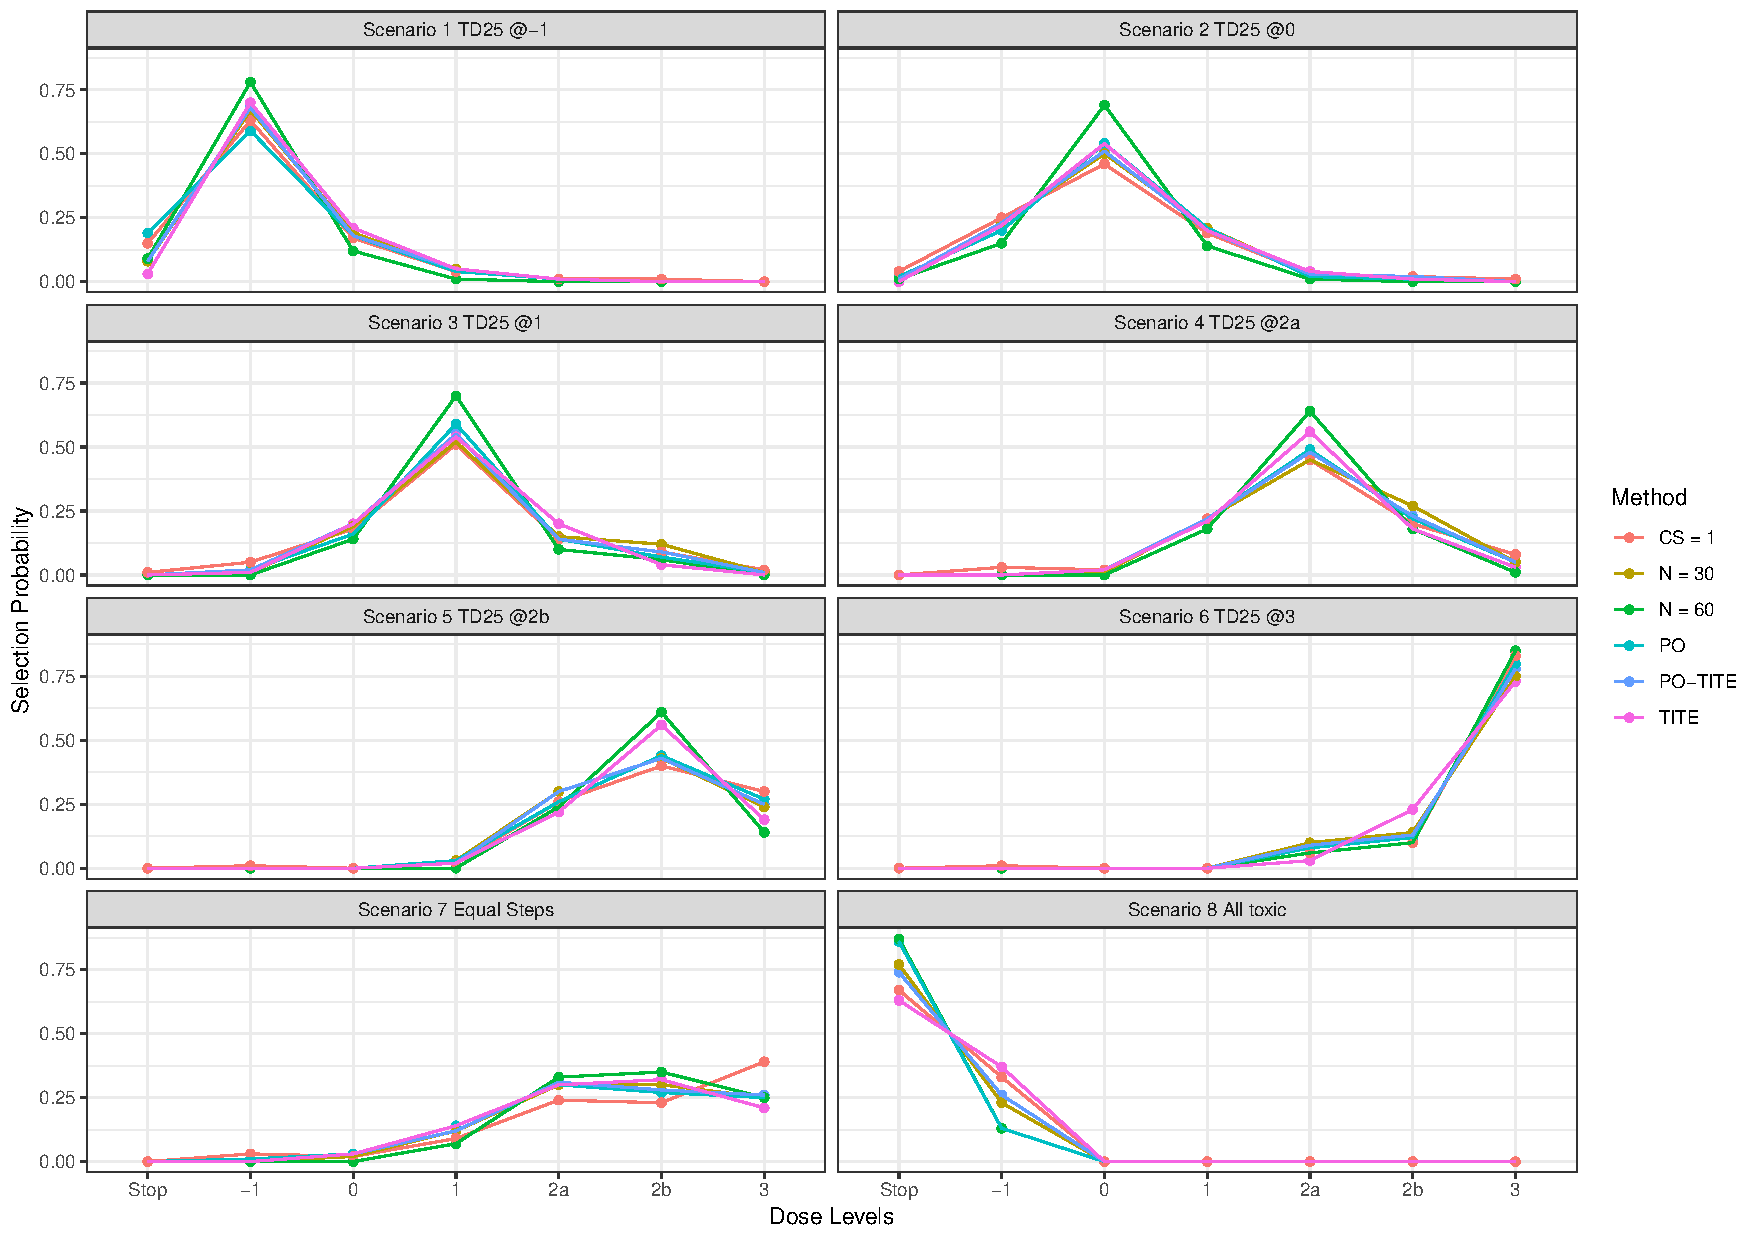
\includegraphics[width=\textwidth]{Adept-SimsOrder1}
\end{figure}

\begin{figure}[h!]
	\centering
	\caption[Plot of simulations comparing designs for ordering 2.]{Plot of the simulation results presented in Table \ref{tab_adept:Design_Comparison2} detailing selection probabilities for multiple designs across scenarios 9-16 (where 2a is considered more toxic than 2b).}
	\label{fig_adept:sims_order2}
	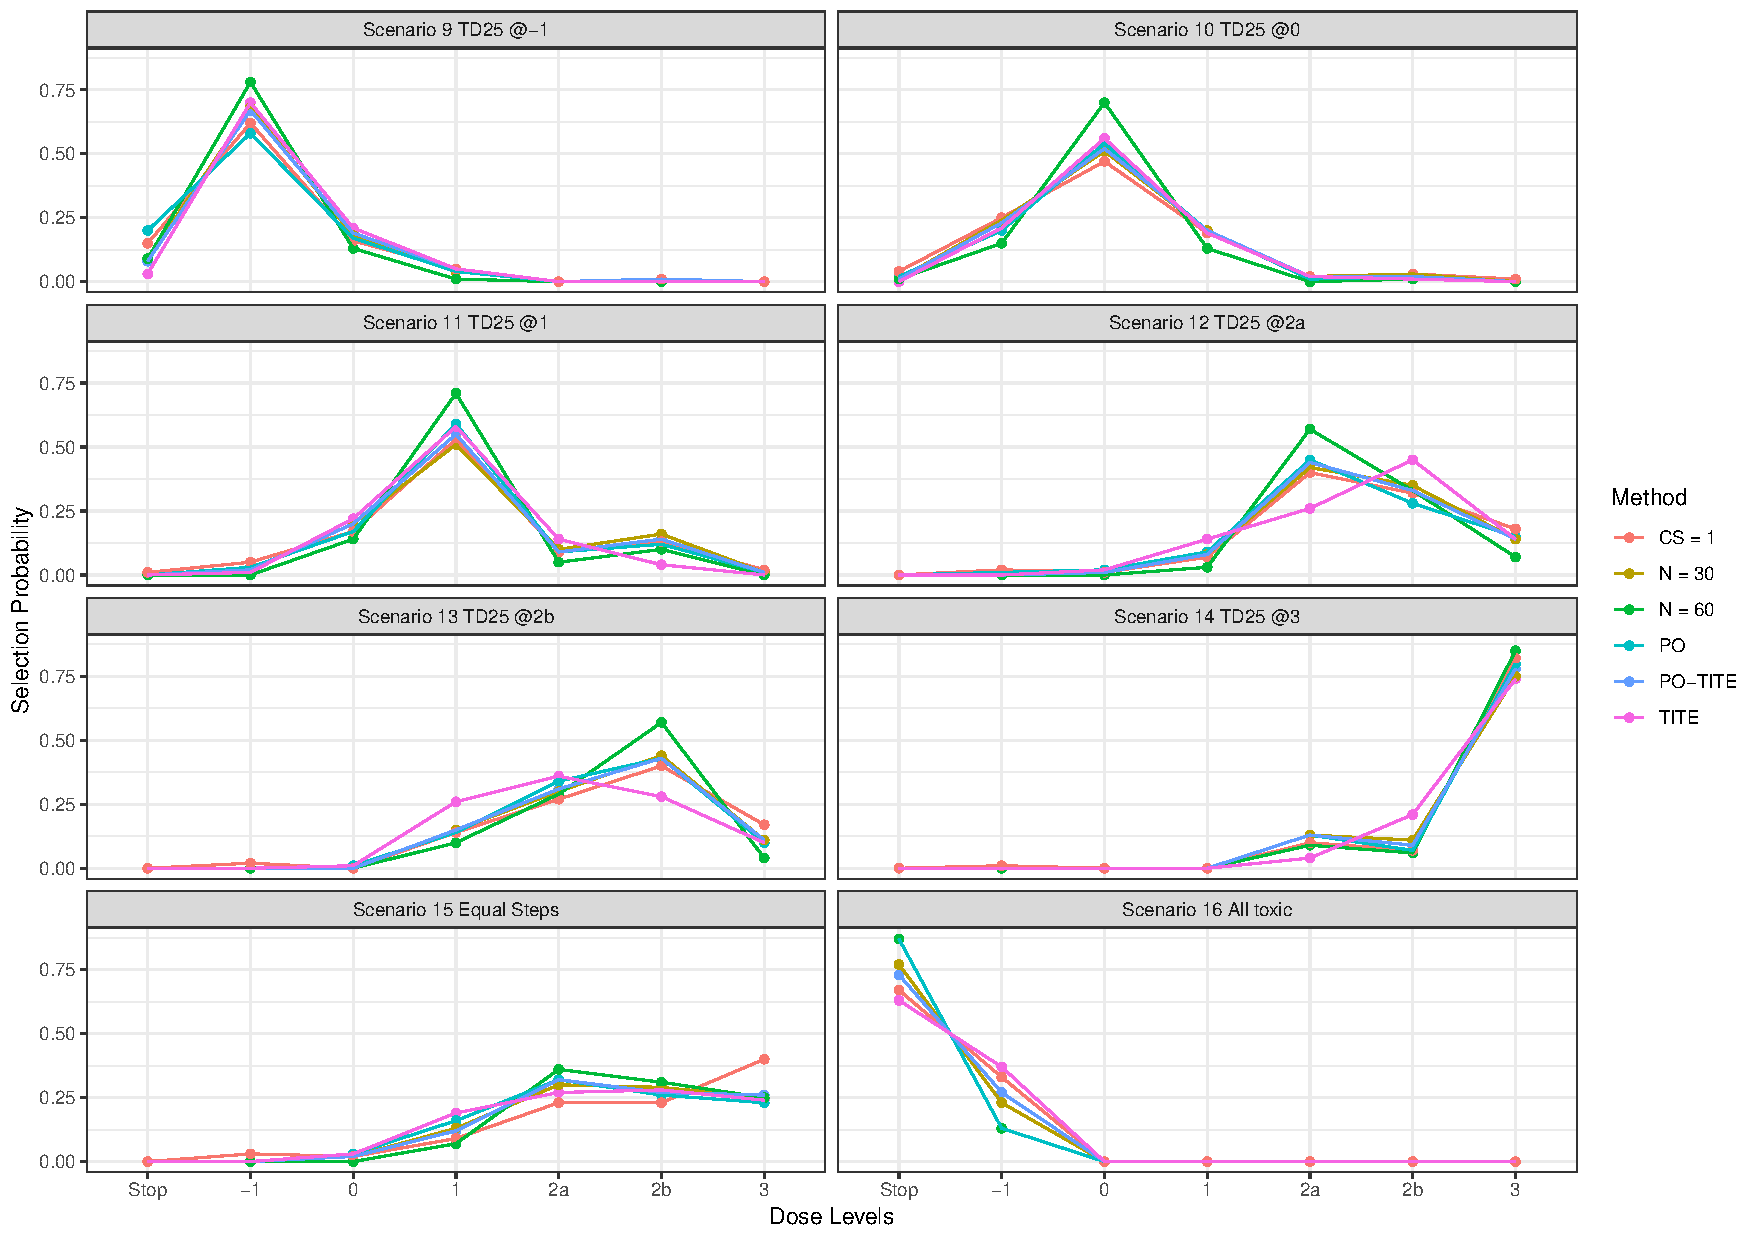
\includegraphics[width=\textwidth]{Adept-SimsOrder2}
\end{figure}

The TITE-CRM performs similarly to our original design for scenarios 1-8 where 2a is assumed less toxic than 2b (Table \ref{tab_adept:OCorder1}). Compared to the PO-TITE design we see increases in probability selection for scenarios 4 and 5 where the target dose is at 2a and 2b respectively. This increase in performance can be attributed to the fact that the partial ordering no longer exists as we have assumed an ordering. The lower selection probabilities for the PO-TITE-CRM can be seen as the price to pay for the uncertainty of not knowing the order of 2a and 2b. However, the TITE-CRM underperforms in scenarios 9-16 where 2a is assumed more toxic than 2b. Specifically, scenarios 12 and 13 where it fails to identify the TD25 the majority of the time. 

The PO-CRM design without a TITE component also performs similarly except for scenarios 1, 8, 9 and 16 where the trial stops more regularly for excess toxicity at the lowest dose. This would be because patients complete the full follow-up window before the next dose allocation decision is made. In a TITE setting a new cohort could be recruited before patients in previous cohorts experience a DLT. The main difference between these designs is the trial duration. Without the TITE component the trial duration is significantly longer, with the average length ranging from 70 to 195 months compared to 39 to 71 months for PO-TITE-CRM. 

The design with a fixed sample size of 30 performs is comparable to our design with the sample size of 60 and the consensus stopping rule. With a sample size of 30 selection probabilities are only 2-5\% lower. For the design with 60 patients, we see much improved operating characteristics with selection probabilities ranging from 31\% to 85\% for the various scenarios. Even though our original design specifies a sample size of 60 we rarely ever reach it as we often stop for consensus hence why this design performs better. The trade-off here is trial duration. Recruitment and follow-up under the constraints of these simulations will take much longer compared to our specification which is not ideal for an early-phase trial. Originally our design had a fixed sample size of 30 but as the clinicians wanted a dose expansion cohort we opted to use the consensus rule to ensure a minimum number of patients would be treated at the TD25. 

For the design with no cohorts, or cohort size of one, we see somewhat comparable performance to that of the PO-TITE-CRM design. The design performs similarly for scenarios where the TD25 is at the lowest or highest dose level but underperforms for the more complex scenarios in terms of selection probabilities. This discrepancy in performance may be related to how the simulations recruit patients into the trial and the large DLT follow-up period. Meaning more frequent dose allocation decisions are being made each with less available information. This also leads to the no cohorts design having a longer duration. Patients entered into the trial in cohorts of three won't having to wait the full minimum follow-up period between patients within the cohort.



%----------------------------------------------------------------------------------------
%	SECTION 5
%-------------------------.

\section{Discussion}  
\label{adept:Discussion}

The PO-CRM and PO-TITE-CRM designs offer solutions to the issue of partial ordering where the order of the treatments is only partially known. The original methodology details that this issue commonly arises in trials of multiple agents, where each drug individually may follow the monotonicity assumption but when combined at certain dose levels this may not hold. This issue is typically dealt with by fixing the dose of one of the agents and escalating in the other or escalating in both agents simultaneously. This means certain drug combinations that are clinically relevant may not be investigated or even considered.  
 
Here we have shown that these issues can also arise in other situations. Even though the ADePT-DDR trial uses multiple agents the issue of partial ordering still occurs due to the varying treatment dose and schedule for one of its agents AZD6738. Implementing the PO-TITE-CRM design allowed us to deal with this issue effectively. There may be other factors or variables in single-agent dose-finding trials that would lead to the issue of partial ordering and would warrant the use of either PO-CRM or PO-TITE-CRM. The small literature review conducted highlighted this may be the first instance of the PO-TITE-CRM design being applied. It is important to note that although this methodology takes into account all the various orderings the main aim is to identify the TD and does not attempt to identify the order that is more correct. 

Compared to other CRM based designs only a few additional pieces of information are required to implement the PO-CRM design. More importantly is the number of toxicity orderings and prior probabilities for the orders. Dependent on how many dose combinations are available it may not be feasible to investigate all combinations and all orderings. Careful thought and consideration should be given to the combinations and orderings selected which would require input from all relevant investigators. In terms of priors for orderings if no prior information is available all orders should be treated as equally likely to occur. Extending this design to the PO-TITE-CRM requires a fit for purpose weight function and is applied similarly to the TITE-CRM methodology. There is an R package available with functions that can be used to run and simulate a PO-CRM trial. These functions were extended to included weighted dose toxicity models as described in this chapter to implement PO-TITE-CRM into ADePT-DDR. The lack of available software for PO-TITE-CRM specifically may be one of the reasons for its lack of use.

In terms of ADePT-DDR, dose combinations were decided upon by the clinical investigators. The issue of partial ordering was due to the dose-levels 2a and 2b as such this methodology was employed to deal with that scenario. Meaning that this is a very simple example of partial ordering as we only have two possible orderings and six dose levels. The necessity of implementing this methodology was discussed and whether or not adopting an easier solution by simply altering the dose levels would have been better. Ultimately, the dose levels selected by the clinicians were deemed the most relevant with the TD25 likely to be one of these doses.     
 
Simulations and operating characteristics were the main tools used to assess the designs performance as well as help understand the impact of sample size and stopping rules. This was an iterative process that involved running multiple iterations of simulations under various scenarios until the design was finalised. A key point is that scenarios from simulations should account for each of the possible orderings. ADePT-DDR only has two orderings, we ran scenarios for both. For a trial with a greater number of orderings, this may be unfeasible but at least some scenarios should be assessed to ensure the design is behaving as expected. Overall, the design operating characteristics performed reasonably well even in difficult scenarios. 

One limitation of the simulations is how the time-to-event data is generated. The time of DLTs is sampled from a uniform distribution $U(0, 413)$, where the time of the DLT can occur at any time between the patient beginning treatment and the end of follow-up (413 days). Using this uniform distribution implies that a DLT has an equal probability of occurring at any time-point in the observation window. This may not be an accurate representation of what happens in the actual trial. Similar comments can be made about the accrual rate used in the simulations. Here we specified the recruitment of one patient per month which is in no way guaranteed for the actual trial. Wages et al. \cite{wagesUsingTimetoeventContinual2013}, when presenting this methodology investigated four different applications of the PO-TITE-CRM which used different models to enroll patients and allocate DLTs. Results across these four applications were comparable. 

The simulations are also able to instantaneously determine dose-levels for incoming cohorts with all available information. This does not fully reflect the process in which dose-escalation decisions would be made during the actual running of the trial. The analysis would require a data snapshot and time would have to be spent cleaning the data and determining the next dose-level. Meaning any data from the point of the snapshot would not be included in any dose escalation/de-escalation decisions. 

Similarly, there may also be limitations with some of the design choices made concerning to cohort size and sample size. These were investigated alongside a variety of other trial designs that could have been implemented. This was done to validate the choices we made with the design and highlight the differences in operating characteristics due to the varying assumptions and components in the designs. The standard PO-CRM had a much longer average duration due to the lack of TITE component whereas a standard TITE-CRM overall performs better but assumes the ordering of toxicity is known. 


%----------------------------------------------------------------------------------------
%	SECTION 6
%-------------------------.

\section{Conclusion}  
\label{adept:Conclusion}

The monotonicity assumption may not hold in some dose-finding trials leading to the issue of partial ordering. This could be due to multiple-agents being investigated or varying factors in single-agent treatment. PO-CRM and PO-TITE-CRM are important trial designs as they address this core issue. ADePT-DDR is a platform trial with its initial component being a dose-finding trial investigating AZD6738 in combination with radiotherapy, of which the toxicity ordering for two of the dose levels for investigation is unknown. The PO-TITE-CRM design allows for us to deal with this issue of partial ordering as well as account for potential late-onset toxicities due to radiotherapy with its TITE component. 

We detail the issue of partial ordering and how we implemented the trial design, in what we believe is the first real-world application of this design. A large amount of simulation work is required to assess the performance of the design. This is often an iterative process to refine decisions that were made and often requires input from both clinical and statistical investigators. We recommend running several varied scenarios for each potential ordering that will be investigated. Finally, we also compared the implementation of PO-TITE-CRM to various other designs. 

 
% Chapter Template

\chapter{Extensions to the Wages and Tait trial design} % Main chapter title

\label{WT} % For referencing this chapter elsewhere, use \ref{WT}

%----------------------------------------------------------------------------------------
%	SECTION 1
%----------------------------------------------------------------------------------------

\section{Introduction}
\label{WT:Introduction}

Typically the main aim of Phase \RN{1} clinical trials is to identify the maximum tolerated dose (MTD) of the treatment being investigated. The MTD is usually determined under the cytotoxic assumption which assumes the most toxic dose is the most efficacious. With model-based designs such as the continual reassessment method (CRM) \cite{oquigleyContinualReassessmentMethod1990} escalation occurs to identify the dose with an associated probability of toxicity based on a pre-defined target. Dose selection and escalation decisions do not consider efficacy rather they are determined based on the occurrence of toxicities. The cytotoxic assumption here implies that the rate of efficacy increases monotonically with the dose-level and probability of toxicity. Subsequent Phase \RN{2} trials aim to assess the efficacy of the treatment at the recommended dose (MTD). Usually, these two phases are conducted independently of each other and as such, the ability to share information across the phases is somewhat lost. 

For treatments like chemotherapy which kills all cells including cancer cells \cite{corrieCytotoxicChemotherapyClinical2008}, the cytotoxic assumption is valid. However, the emergence of modern treatments such as immunotherapy and molecular targeted agents challenges this paradigm. Immunotherapy is a form of treatment that utilises the body's immune system to fight cancer \cite{mellmanCancerImmunotherapyComes2011}. Molecular targeted agents (MTA) work by interfering with specific molecules responsible for the growth, spread, and progression of cancer \cite{soriaAddedValueMolecular2011}. The monotonic assumption of dose-efficacy may not hold for these new types of treatments. Furthermore, these treatments, in general, are less toxic than traditional cytotoxic agents such as chemotherapy therefore it is possible the most efficacious dose may occur at a dose-level below the MTD \cite{ahnOptimalBiologicalDose2016}. This produces some methodological challenges for dose-finding trials. Instead of trying to identify the MTD, the goal would be to determine the optimal biological dose (OBD). Depending on the aims of the trial and the design implemented the definition of the OBD may vary. The OBD could be a dose that provides the maximum probability of efficacy with the probability of toxicity being less than a pre-defined target value, or the dose that has a beneficial trade-off between toxicity and efficacy. To determine an optimal dose both toxicity and efficacy outcomes need to be considered and this leads to a need for joint phase \RN{1}/\RN{2} trial designs. Here we will briefly explore some of these designs. 

Braun \cite{braunBivariateContinualReassessment2002} proposed the bivariate continual reassessment method (bCRM), an extension to the CRM which incorporates competing outcomes for both toxicity and disease progression. The design models the probabilities of toxicity and progression independently, it is suggested that either empiric, logistic, or hyperbolic tangent functions are used dependent on their biological plausibility. Both outcomes are then combined into a joint distribution which is used to estimate posterior means based on priors and observed data. 

Thall \& Cook \cite{thallDosefindingBasedEfficacytoxicity2004} developed EffTox, a Bayesian adaptive dose-finding trial based on trade-offs between the probabilities of toxicity and efficacy. Marginal probabilities of efficacy and toxicity at each dose are modelled and used with utility contours to determine the desirability of each dose based on posterior probabilities of efficacy and toxicity \cite{brockImplementingEffToxDosefinding2017}. 

Zhou et al. \cite{zhouUtilitybasedBayesianOptimal2019} introduced a Utility-based Bayesian Optimal Interval (U-BOIN) phase \RN{1}/\RN{2} design to identify the OBD. This design is an extension of the Bayesian optimal interval (BOIN) design for phase \RN{1} trials developed by Liu and Yuan \cite{liuBAYESIANDATAAUGMENTATION2013}. U-BOIN jointly models toxicity and efficacy with a multinomial-Dirichlet model and uses a utility function to measure the dose risk-benefit trade-off. The design consists of two seamless stages. Firstly, in stage \RN{1} the BOIN design is used to explore the dose levels and determine a set of admissible doses and collect preliminary efficacy data. In stage \RN{2} posterior estimates of utility for each dose are continuously updated after each cohort using toxicity and efficacy data from both stages. 

Zhang et al. \cite{zhangAdaptiveDosefindingDesign2006} introduced the trivariate CRM (TriCRM) design. The design considers patients to have one of three possible outcomes: no efficacy and toxicity, efficacy without toxicity, and toxicity. These outcomes are then modelled using a continuation-ratio model. A Bayesian approach and dose-finding algorithm are then used to identify the OBD similar to the CRM.  

Anathakrishnan et al. \cite{ananthakrishnanExtensionsMTPITEQR2018} produced extensions to the modified Toxicity Probability Interval (mTPI) design by Ji \& Wang \cite{jiModifiedToxicityProbability2013} and Toxicity Equivalent Range (TEQR) design by Blanchard \& Longmate \cite{blanchardToxicityEquivalenceRange2011} to include efficacy outcomes. In both designs, isotonic regression is applied to the observed DLT rates at the end of the trial. Dependent on the shapes of the dose-response curves and the underlying response rates isotonic regression is applied to the observed response rates or the differences in observed response rates to determine the optimal dose. 

Riviere et al. \cite{rivierePhaseIIDosefinding2018} developed a Bayesian dose-finding design for MTA. The design works on the premise that for MTA efficacy initially increases with dose then eventually plateaus. They use a logistic model with a plateau parameter to capture the dose-level at which plateaus begin in the dose-efficacy relationship. A weighted likelihood approach is also used to accommodate for any potential late-onset toxicities. This methodology incorporates adaptive randomisation to allocate patients to the dose-level closest to the likely plateau point.

This chapter revolves around the seamless phase \RN{1}/\RN{2} dose-finding adaptive design by Wages and Tait \cite{wagesSeamlessPhaseII2015}, which we will refer to as the WT design. This design models toxicity and efficacy independently. To model the probability of efficacy a set of possible efficacy skeletons are considered which would correspond to plausible dose-efficacy relationships. For the class of dose-efficacy models, a single parameter model is used similar to the empiric model of the CRM. The authors recommend that ($2n - 1$) efficacy skeletons are specified where $n$ is the number of doses being investigated. Toxicity is modelled using a CRM approach with an empiric model. As such a skeleton for toxicity is also required for this design. The dose-finding operates in two stages the adaptive randomisation (AR) phase and the maximisation phase. In the AR phase patients are adaptively randomised amongst a set of tolerable doses (determined by the CRM toxicity model), where probabilities of randomisation to each dose are proportional to their posterior probabilities of efficacy. A pre-defined number of patients enter the AR phase and once recruitment has been completed we move to the maximisation phase. In this phase, patients are allocated to the dose in the tolerable set which maximises the probability of efficacy.  

The incorporation of an AR phase early on into the trial is beneficial since there may be a lack of data to rely on decisions made by the maximisation of efficacy probabilities. Also, there may be doses that haven't been tested and randomisation allows for information to be collected from these. It also helps avoid getting stuck repeatedly recruiting to the same dose and allows for a more broad understanding of the dose-efficacy and toxicity relationships. One extension we propose is the inclusion of randomisation to a control arm in the design. This would provide a set of patients who receive standard of care to act as controls and allow for comparisons to be made with outcomes from patients receiving the OBD. There is also the added benefit of being able to include standard of care into the models to get a better understanding of the dose-efficacy and toxicity relationships.  

Section \ref{WT:Wages-and-Tait-Design}, details the statistical aspects of the WT design and how it works. We introduce our extension to the design to include randomisation to control in Section \ref{WT:RtC-WT}. Section \ref{WT:Evaluation-of-the-Extension} evaluates the performance of the new design with a simulation study. Finally, we finish with a discussion in Section \ref{WT:Discussion}.  


%----------------------------------------------------------------------------------------
%	SECTION 2
%----------------------------------------------------------------------------------------
\section{The Wages and Tait Design}
\label{WT:Wages-and-Tait-Design}

In this section, we detail the Wages and Tait design using the same notation as presented in their paper \cite{wagesSeamlessPhaseII2015}. A set of $I$ doses under investigation can be denoted as $\mathscrsfs{D} = \{d_1, ...,d_i\}$. For each patient $j$ entered into the trial they are allocated to a dose-level and joint outcomes for toxicity and efficacy are measured. The dose for the $j$th patient, $X_j$, $j = 1,...n$ can be thought of as random, taking values $x_j \in  \mathscrsfs{D}$. Let $Y_j$ and $Z_j$ be the random variables for binary toxicity and efficacy events respectively. For an individual patient $j$, toxicity and efficacy outcomes can take values $y_j, z_j \in \{0,1\}$ where 0 indicates an event didn't happen and 1 indicates that it did. 

Wages and Tait \cite{wagesSeamlessPhaseII2015} utilise the CRM approach of O'Quigley et al. \cite{oquigleyContinualReassessmentMethod1990} to model toxicity. A univariate Bayesian method is used which begins by assuming a monotonically increasing dose-toxicity curve. The DLT probabilities, $\pi_T(d_i)$, are modelled at each dose level $i$ where $i= 1, ..., I$. The power model is specifically used by Wages and Tait in this design given by 

\begin{equation}
	\label{WT:eq_power-model}
	F(d_i, \beta) = p_i^{exp(\beta)}.
\end{equation}

A working model or skeleton containing the prior beliefs of toxicity at each dose-level is required in the form $0 < p_1 < ... <p_I <1$. For the single parameter in the power model $\beta$ we assume it has a prior distribution $g(\beta)$. After the inclusion of $j$ subjects into the trial, we have  data in the form of $\Omega_j = \{(x_1,y_1,z_1), ..., (x_j,y_j,z_j)\}$. The toxicity data can be used with Equation \ref{WT:eq_power-model} to give the likelihood for $\beta$

\begin{equation}
	L(\beta|\Omega_j)=\prod_{l=1}^{j}\{F(x_l,\beta)\}^{y_l}\{1-F(x_l,\beta)\}^{1-y_l},  
\end{equation}

the posterior density for $\beta$ can be calculated using  

\begin{equation}
	P(\beta|\Omega_j) = \frac{L(\beta|\Omega_j)g(\beta)}{\int_{-\infty}^{\infty}L(\beta|\Omega_j)g(\beta)d\beta}. 
\end{equation}

This can then be used to establish the posterior mean of $\beta$

\begin{equation}
	\hat{\beta}_j = \int_{-\infty}^{\infty}\beta P(\beta|\Omega_j)d\beta.
\end{equation} 

Using $\hat{\beta}_j$ estimates of DLT probabilities at each dose level can be obtained via 

\begin{equation}
	\hat{\pi}_T(d_i) = F(d_i, \hat{\beta}_j) = p_i^{exp(\hat{\beta}_j)}. 
\end{equation}

For a specific maximum acceptable toxicity rate, $\phi_T$ a set of acceptable or admissible doses can be declared as follows

\begin{equation}
	\mathscrsfs{A}_j = \{d_i : \hat{\pi}_T(d_i)  \leq \phi_T ; i = 1,...,I \}.
\end{equation} 

To model efficacy, a Bayesian approach is taken similar to how toxicity was modelled but rather than using a singular working model a class of working models is considered. They use a class of skeletons that correspond to various dose-efficacy relationships. These relationships might be monotonically increasing (as the dose-levels increase efficacy increases), unimodal (initially increasing then decreasing) or plateau (initially increase then level off). As a guide, it is suggested that $(2I-1)$ working models should be specified. The probability of an efficacious response at dose $d_i$ is denoted as $\pi_E(d_i)$. The primary aim of the trial is to identify the optimal dose $d_v \in \mathscrsfs{D}$ which is defined such that 

\begin{equation}
	\pi_E(d_1) \leq ... \leq \pi_E(d_v) \geq ... \geq \pi_E(d_I). 
\end{equation}

Let $K$ denote the number of efficacy skeletons being used. Then for each skeleton $k$ we have $0 < q_{1k} < ... <q_{Ik} <1$ and for a particular skeleton $k; k = 1,...,K$ the true probability of efficacious response $\pi_E(d_i)$ at $d_i$ is modelled by 

\begin{equation}
	\pi_E(d_i) = Pr(Z_j = 1|d_i) \approx G_k(d_i,\theta) = q_{ik} ^{exp(\theta)}.
\end{equation}

As with the modelling of toxicity the power model is used again. Similarly as with $\beta$ a prior distribution $h(\theta)$ is assumed for $\theta$. For both the toxicity and efficacy models a Normal prior is used as first suggested by O'Quigley and Shen \cite{oquigleyContinualReassessmentMethod1996} such that $\beta, \theta \sim N(0,1.34)$. Additionally for the modelling of efficacy prior information regarding the plausibility of each model is taken into account using a weight function $\upsilon(k) = \{\upsilon(1), ..., \upsilon(K)\}$, where $\upsilon(k) \geq 0$ and where $\sum_k \upsilon(k) = 1$. If no information is available a discrete uniform distribution can be specified for $\upsilon(k)$. After $j$ patients have been included and observed in the study we have efficacy data from $\Omega_j$ and the likelihood model under $k$ is given by 

\begin{equation}
	L(\theta|\Omega_j)=\prod_{l=1}^{j}\{G_k(x_l,\theta)\}^{z_l}\{1-G_k(x_l,\theta)\}^{1-z_l},  
\end{equation}

the posterior density is 

\begin{equation}
	P(\theta|\Omega_j) = \frac{L(\theta|\Omega_j)h(\theta)}{\int_{-\infty}^{\infty}L(\theta|\Omega_j)h(\theta)d\theta},
\end{equation}

and under skeleton $k$ the posterior mean is given by 

\begin{equation}
	\hat{\theta}_{jk} = \int_{-\infty}^{\infty}\theta P(\theta|\Omega_j)d\theta.
\end{equation} 

This information can be used to establish posterior model probabilities 

\begin{equation}
	w(k|\Omega_j) = \frac{\upsilon(k)\int_{-\infty}^{\infty}L_k(\theta|\Omega_j)h(\theta)d\theta}{\sum_{k=1}^{K}\upsilon(k)\int_{-\infty}^{\infty}L_k(\theta|\Omega_j)h(\theta)d\theta}.
\end{equation}

The posterior model probabilities are then used to determine which skeleton will be selected to model the dose-efficacy relationship. Each time a new patient is to be entered into the study and a dose-escalation decision needs to be a made, the skeleton $k^*$ with the largest posterior probability is selected such that

\begin{equation}
	k^* = arg \; \underset{k}{max}w(k|\Omega_j).
\end{equation}

After determining the best skeleton and calculating the posterior mean of $\theta$ estimates of efficacy probabilities are then generated for each dose. 

\begin{equation}
	\hat{\pi}_E(d_i) = G_{k^*} (d_i, \hat{\theta}_{jk^*})
\end{equation}

Dose-finding is conducted in two stages. The first stage begins with the adaptive randomisation (AR) phase. Here the next dose is randomly selected from the set of admissible doses determined by the CRM toxicity model. Randomisation probabilities for each dose are proportional to $\hat{\pi}_E(d_i)$ so that doses with higher estimated efficacy are more likely to be assigned to patients. For doses in $\mathscrsfs{A}_j$ their adaptive randomisation probability $R_i$ is 

\begin{equation}
	\label{WT:eq_WT-ARprob}
	R_i = \frac{\hat{\pi}_E(d_i)}{\sum_{d_i \in \mathscrsfs{A}_j}\hat{\pi}_E(d_i)}. 
\end{equation}

The AR phase lasts for a subset of $j_R$ patients such that $j_R \leq J$, where $J$ is the total number of patients to be entered into the trial. Wages and Tait suggest as a general rule of thumb to allocate 50\% of patients to both stages. It was shown that this approach works well in a variety of scenarios. However, this can be easily be adapted to suit individual trials. 

Once the AR phase has been completed the design switches to the second stage called the maximisation phase. Here the next dose is the dose from the admissible set with the highest estimated probability of efficacy. For a dose-escalation decision that needs to be made in the maximisation phase for the $(j+1)$th patient the dose $x_{j+1}$ is selected from the admissible set of doses $\mathscrsfs{A}_j$ with the highest estimated efficacy probability $\hat{\pi}_E(d_i)$ i.e. 

\begin{equation}
	x_{j+1} = arg \; \underset{d_i \in \mathscrsfs{A}_j}{max}\hat{\pi}_E(d_i)
\end{equation}

The design also incorporates stopping rules for safety and futility. The safety rule stops the trial if too much toxicity is observed at the lowest dose level. This rule is applied throughout the trial for each dose-escalation decision. Exact binomial 95\% confidence intervals are calculated for the lowest dose. The lower bound of the interval is then compared to the acceptable toxicity rate $\phi_T$. If the lower bound interval is greater than the acceptable rate it can be said that the treatment is too toxic to warrant further investigation. Patients need to have been observed at the lowest dose for this rule to trigger, if there is no data available at the lowest dose the binomial confidence interval is effectively 0. 

The futility rule stops the trial if there are too few observed efficacy events. This rule only comes into play during the maximisation phase. This rule uses a similar method to the stopping rule by utilising binomial 95\% confidence intervals. During the maximisation phase, the dose with the highest probability of efficacy is selected. At this point, the 95\% binomial confidence interval is calculated for the current dose and if the upper bound is less than the futility threshold $\phi_E$ the trial is stopped as the treatment is inefficacious at all doses. Although 95\% confidence intervals are used by Wages and Tait these can be altered accordingly. 


%----------------------------------------------------------------------------------------
%	SECTION 3
%----------------------------------------------------------------------------------------
\section{RtC-WT: An extension to the Wages and Tait Design}
\label{WT:RtC-WT}

In this section, we introduce our proposed extension to the Wages and Tait (WT) design named Randomisation to Control Wages and Tait (RtC-WT). As the name states, the design will allow investigators to utilise the WT design with the ability to recruit patients to a control arm/dose-level. This idea was initially conceived by Kristian Brock (KB) whilst working on the design of a new dose-finding trial.  

%-----------------------------------
%	SUBSECTION 3.1
%-----------------------------------
\subsection{The Rationale for Incorporating Randomisation to Control}
\label{WT:Rationale-for-RtC-WT}

Typically, seamless phase \RN{1}/\RN{2} trial designs perform the tasks of phase \RN{1} and phase \RN{2} trials. However, they do not replace the need for randomised phase \RN{2} trials entirely where preliminary efficacy data is collected on an experimental treatment versus control to determine the need for a larger phase \RN{3} study \cite{yinClinicalTrialDesign2012}. This is our main motivation for introducing RtC-WT. By introducing the ability to randomise to control in the Wages and Tait method we can achieve similar objectives to randomised phase \RN{2} studies. 

An example of where this design may be beneficial is in the investigation of a standard of care treatment in combination with an experimental treatment. The standard of care treatment could be included as the control dose and should have a well-understood toxicity and efficacy profile which could be incorporated into the toxicity and efficacy skeletons. Further dose levels would also receive standard of care along with increasing levels of the experimental treatment, here the interaction between the two treatments in terms of toxicity and efficacy could be investigated and an OBD could be found using the RtC-WT design. 

As a seamless phase \RN{1}/\RN{2} design WT is relatively simple and effective. The familiarity of using a CRM design to model toxicity and naturally extending that methodology to model efficacy with multiple working models mean the design is not particularly difficult to implement. The mathematics behind the design is also not too intense so extensive computation won't be necessary. Given some effort, this design could be implemented in a variety of programming languages although Brock offers easy implementation of this design in his R package escalation \cite{brockModularApproachDose2020}. Considering all these factors extensions to this design can be executed without too many obstacles.

The WT design can be considered fairly unique due to its use of adaptive randomisation. Whilst adaptive randomisation is not the core focus of the design it is still a distinguishing factor that could be leveraged to help investigators answer questions other designs can't. Specifically, the randomisation allows for more dose-levels to be explored and perhaps obtain a better understanding of the dose-toxicity and efficacy relationships. 

Conceptually the WT design could include a control arm without any modification to the design. All that this would require is the addition of a new dose-level at which patients receive control treatment/standard of care. This would need to be implemented as the lowest dose-level as dose-levels still need to obey the monotonicity assumption for toxicity. The issue with taking this approach is that the design is unlikely to allocate patients to the control dose-level. Even though adaptive randomisation is in play the randomisation probabilities are based on estimates of efficacy probabilities and control patients may be unexpected to have an efficacious event. This is a desirable characteristic when investigating treatments as we don't want to allocate too many patients to inefficacious doses. However, if the aim is to establish a cohort of patients as controls to facilitate comparisons to the OBD this is not an optimal characteristic. 

\begin{figure}[!h]
	\centering
	\caption[Flowchart of a two arm randomised dose-finding trial.]{Flowchart of how a two arm randomised dose-finding design would operate using the Wages and Tait design.}
	\label{fig_wt:TwoArmExample}
	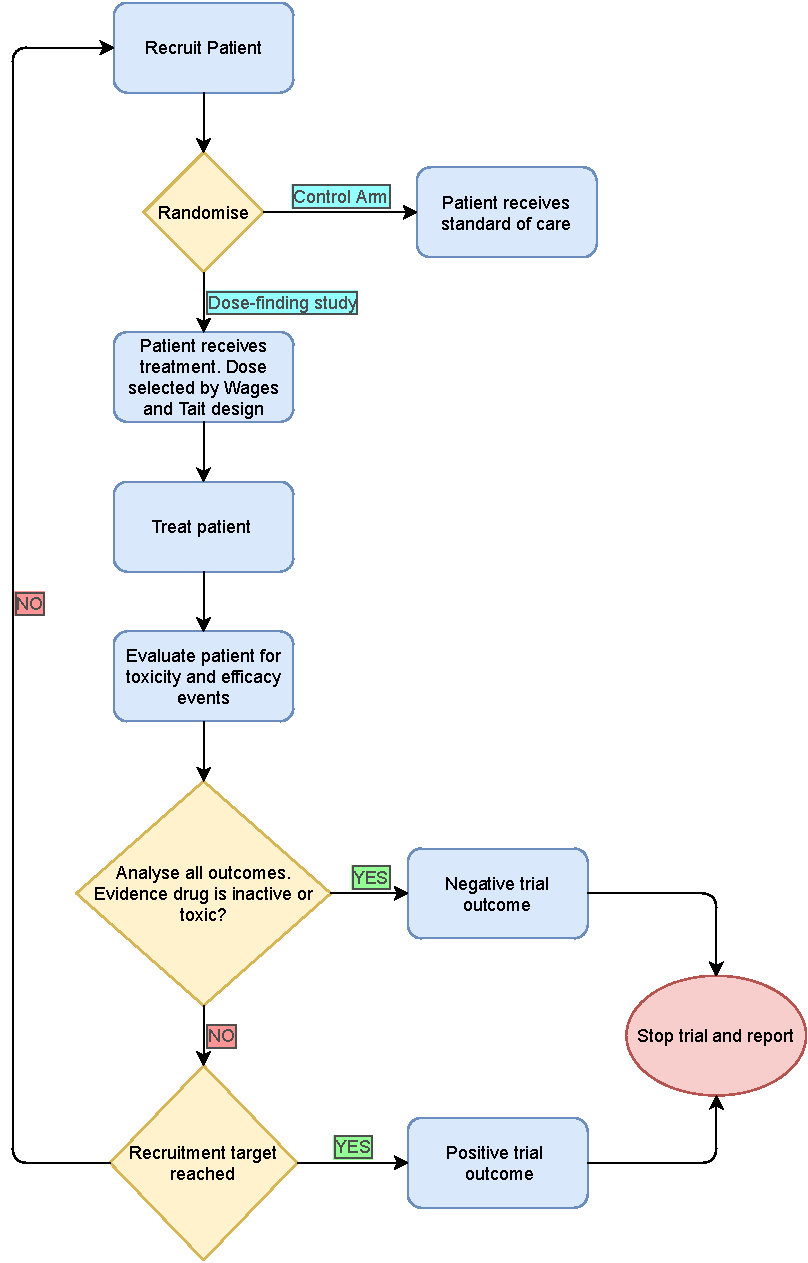
\includegraphics[width=0.77\textwidth]{WT-TwoArmExample}
\end{figure}

There is another approach that could also be used to include a control arm rather than our proposed design RtC-WT. A two-arm randomised design could be used where patients are allocated to either a control arm or a dose-finding arm. Those patients allocated in the dose-finding arm will then be a part of the WT design see Figure \ref{fig_wt:TwoArmExample}. This approach maintains many of the traditional qualities of a two-arm randomised trial. The number of patients in each arm can be specified this way and we guarantee a minimum number of patients in our control arm. Also, the characteristics of patients in both arms are likely to be similar which would be beneficial when making comparisons between the two arms. A downside of this method is that the data for control patients are no longer included in the modelling process. Whilst control patients may still be observed for efficacious and toxic events these won't be included in the modelling as such the ability to make inferences on the dose-toxicity and efficacy relationships in reference to a control/ standard of care dose is lost. 

Both of these approaches have their merit but also have flaws as well. RtC-WT is somewhat of a middle ground that aims to recruit patients to a control dose and include the control patients' data in the modelling process all whilst maintaining reasonable operating characteristics. We detail RtC-WT in Section \ref{WT:Design-RtC-WT} and explore the operating characteristics of this design in Section \ref{WT:Evaluation-of-the-Extension}.

%-----------------------------------
%	SUBSECTION 3.2
%-----------------------------------
\subsection{Design of the Proposed Extension RtC-WT}
\label{WT:Design-RtC-WT}

With this extension, much of the Wages and Tait design stays the same. The modification only impacts the adaptive randomisation (AR) phase and requires some additional specifications at the start of the trial. Firstly, we set the lowest dose-level $d_1$ to be the control dose-level. This dose-level should be included in the working models for efficacy and toxicity and should be treated like any other dose-level. Even if toxicity and efficacy events are expected to be non-existent for control their corresponding skeleton values must be non-zero. Investigators also need to consider a randomisation probability $\phi_R$ for the control dose. During the AR phase, $\phi_R$ represents the probability of selecting the control dose as the next dose level. The probability of randomisation $R_i$ for other dose in $\mathscrsfs{A}_j$ is scaled accordingly such that the $\sum_{d_i \in \mathscrsfs{A}_j} R_i = 1$. The adaptive randomisation probabilities can now be expressed as 

\begin{equation}
	R_1 = \phi_R,
\end{equation}

\begin{equation}
	R_i = (1-\phi_R)\frac{\hat{\pi}_E(d_i)}{\sum_{d_i \in \mathscrsfs{A}_j}\hat{\pi}_E(d_i)}, \; \; i=2,...,I. 
\end{equation}

Compared to Equation \ref{WT:eq_WT-ARprob} the adaptive randomisation probability is fixed to $\phi_R$ at the lowest dose (the control dose) and for all other dose levels in the admissible set $\mathscrsfs{A}_j$ a scaled randomisation probability is calculated. By fixing the probability for the control dose we guarantee a greater chance of patients being allocated to this dose-level. Although estimates of efficacy at the control dose-level $\hat{\pi}_E(d_1)$ do not directly impact its associated randomisation probability, the efficacy data that generated the estimate is still included in the efficacy modelling and impacts probabilities for the remaining dose-levels. Also, by scaling the remaining probabilities of dose-levels in the admissible set we ensure that those doses with high estimates of efficacy maintain their proportional advantage of selection over the other non-control doses.

Some adjustments were made to the stopping rule for safety. The WT design assesses the lower bound of the 95\% binomial confidence interval of DLT rate for the lowest dose to determine whether or not the trial should be stopped. However, with the RtC-WT design since the lowest dose is the control, it makes little sense to surmise treatment is toxic here since none of the patients on control would have received the experimental treatment. It is also likely the trial would never recommend stopping even if the treatment is toxic since patients on control are unlikely to experience a toxic event. The RtC-WT design stops for safety by checking for excess toxicity at the second-lowest dose-level (the first treatment dose-level).

Once the AR phase ends, dose-levels are no longer selected by adaptive randomisation. At this point, it will be difficult for patients to be recruited to the control dose since recommended doses will be based on those with the greatest estimates of efficacy. As such it is important to consider the values set for both your randomisation probability for control $\phi_R$ and the size of the AR phase $j_R$. Wages and Tait simply suggest a 50:50 split between both the AR phase and the maximisation phase and show relatively good performance at this level. However, for RtC-WT the AR phase is the main component and more thought should be given here. In the next section, we explore multiple combinations to better understand how these choices impact the operating characteristics of the design. We also compare RtC-WT to the two alternative designs mentioned in section  \ref{WT:Rationale-for-RtC-WT} via simulations and the inspection of operating characteristics specifically, the selection probabilities of the OBD and patient allocation numbers at each dose-level. 

%----------------------------------------------------------------------------------------
%	SECTION 4
%----------------------------------------------------------------------------------------
\section{Evaluation and Exploration of the Extension via Simulations}
\label{WT:Evaluation-of-the-Extension}

In this section, we evaluate the performance of RtC-WT in comparison to the two alternative designs mentioned in Section \ref{WT:Rationale-for-RtC-WT}. We also explore the impact of changing the probability of randomisation to control and the number of patients included in the adaptive randomisation phase. These will both be assessed via simulation and inspection of their operating characteristics. To facilitate simulations a generic trial example will be utilised along with a variety of scenarios. 

%-----------------------------------
%	SUBSECTION 4.1
%-----------------------------------
\subsection{Design Specification}
\label{WT:Design-Spec}

Here we detail the design specifications for RtC-WT that we will be using throughout this section. We assume five dose-levels, where the lowest dose is considered to be the control dose-level. The maximum sample size of the trial is set at 60 with patients recruited in cohorts of three and the first cohort starting at dose-level two (the first treatment dose-level). The pre-specified toxicity upper bound and efficacy lower bound are set at $\phi_T = 0.35$ and $\phi_E = 0.50$ respectively. Toxicity and efficacy skeletons, $p_i$ and $q_i$ respectively, are presented in Table \ref{tab_wt:tox-eff-skeleton}. In terms of efficacy relationships monotonic, unimodal and plateau skeletons were all used. We assume that each of the seven efficacy skeletons is equally likely and set $\upsilon(k) = \frac{1}{7}$. 


\begin{table}[!h]
	\centering
	\caption{Toxicity and efficacy skeletons for RtC-WT in the example trial.}
	\label{tab_wt:tox-eff-skeleton}
	\begin{tabular}{c|ccccc}
		\hline
		\multicolumn{1}{c|}{\multirow{2}{*}{\textbf{Skeleton}}} & \multicolumn{5}{c}{\textbf{Dose-levels}}                       \\
		\multicolumn{1}{c|}{}                                   & \textbf{1} & \textbf{2} & \textbf{3} & \textbf{4} & \textbf{5} \\ \hline
		$p_i$    & 0.1 & 0.15 & 0.25 & 0.35 & 0.45 \\
		$q_{i1}$ & 0.3 & 0.7 & 0.6 & 0.5 & 0.4 \\
		$q_{i2}$ & 0.3 & 0.6 & 0.7 & 0.6 & 0.5 \\
		$q_{i3}$ & 0.3 & 0.5 & 0.6 & 0.7 & 0.6 \\
		$q_{i4}$ & 0.3 & 0.4 & 0.5 & 0.6 & 0.7 \\
		$q_{i5}$ & 0.3 & 0.5 & 0.6 & 0.7 & 0.7 \\
		$q_{i6}$ & 0.3 & 0.6 & 0.7 & 0.7 & 0.7 \\
		$q_{i7}$ & 0.3 & 0.7 & 0.7 & 0.7 & 0.7 \\ \hline
	\end{tabular}
\end{table}

For the control dose, we have set our prior beliefs for the probability of toxicity at 10\% and the probability of efficacy at 30\%. This can of course be adjusted if there is reason to believe that the control dose may be slightly more/less effective or toxic. 

Wages and Tait recommend $(2I-1)$ efficacy skeletons be used which in this example would be nine, however, we have only considered seven. As there are only four active doses and we are assuming we understand the control dose in terms of toxicity and probability then seven different skeletons fits in the Wages and Tait's recommendation. Since we don't expect many efficacy events from our lowest dose we removed the two efficacy skeletons with dose-efficacy relationships that suggest the lowest dose would be the most efficacious. For completeness, the first extra skeleton would be unimodal with the highest efficacy occurring at dose-level one (i.e. 0.7, 0.6, 0.5, 0.4, 0.3 for dose-levels 1-5) and the second skeleton would be a plateau relationship with the plateau beginning at dose-level one (i.e. 0.7, 0.7, 0.7, 0.7, 0.7 for dose-levels 1-5). 

We also include the same stopping rules for safety and futility with the safety rule assessing toxicity at dose-level two. A rule will also be implemented to prevent the skipping of untried doses when escalating. This rule does not apply when de-escalating. 

The two parameters we have left to specify are the fixed adaptive randomisation probability for control $\phi_R$ and the number of patients included in the adaptive randomisation phase $j_R$. In Section \ref{WT:Design-RtC-WT} we briefly discussed the importance of giving thought when setting these values. This is due to the fact they are the main things driving how RtC-WT works compared to the standard WT design. For example, one could set the AR phase to last for the whole trial and keep a relatively low probability to randomise to control. Alternatively, the AR phase can be set for half the patients in the trial and double the probability of randomisation could be used. These two approaches could allocate the same number of patients in the control arm but have different operating characteristics. It could be hypothesised that by setting the AR phase for the whole trial you miss out on the maximisation phase where patients are allocated to the estimated most efficacious dose which could yield slightly worse operating characteristics. We explore different combinations of these parameters in the next section. 


%-----------------------------------
%	SUBSECTION 4.2
%-----------------------------------
\subsection{Impact of AR phase size and probability of randomisation to control on RtC-WT}
\label{WT:Impact-ARandRTCon-RtC-WT}


The effect of adjusting the probability of randomising to control $\phi_R$ is fairly intuitive, as the probability increases the percentage chance that patients are allocated to the control dose-level also increases. However, this is only in isolation without considering the size of the AR phase. Increasing the AR phase would also mean more patients are likely allocated to the control dose-level since the randomisation only occurs in the AR phase. The interest lies within the interaction of both of these components and their impacts on operating characteristics. To gain a better understanding of this impact on RtC-WT we consider multiple combinations. 

We look at two different probabilities for randomisation to control, $\phi_R = 0.2$ and $\phi_R = 0.33$ i.e. 20\% and 33\% probability of patients being allocated to the control dose-level during the AR phase of the trial. We also consider varying AR phase sizes, specifically $j_R = 0, 15, 30, 45 ,60$ essentially looking at when the AR phase lasts 0\%, 25\%, 50\%, 75\% and 100\% of the trial. The inclusion of setting the AR phase as 0 is somewhat counter-intuitive since the trial will just be run using the maximisation phase where the most efficacious doses are allocated. As such it is unlikely that the control dose-level would ever be the most efficacious specifically in our scenario here. However, its inclusion will serve as a benchmark as the design most likely to achieve optimal performance in terms of locating the OBD since there will be no randomisation and the estimated most efficacious dose will always be the one being tested. Similarly, by setting the AR phase at 60 we limit some of the designs features by never entering the maximisation phase to select dose levels based on efficacy. Also, the stopping rule for futility doesn't come into play. Although, many more combinations could be explored this set provide a good basis for us to gain a better understanding of how RtC-WT works. It also helps us understand how best to optimise RtC-WT for comparisons with alternative designs later on.  

To compare these different combinations we use simulations covering a wide range of scenarios. For each scenario, we simulate 10000 trials each consisting of 60 patients recruited in cohorts of three. Patient outcomes for toxicity and efficacy are randomly sampled using true toxicity and true efficacy probabilities, these are assumed to be independent of each other. Dose-allocation decisions are made after each cohort of patients and then the subsequent cohort is allocated the recommended dose. The trial could also be stopped here if the recruitment target is reached or if any of the stopping rules are triggered. The rest of the design specification is as defined in Section \ref{WT:Design-Spec}. 

The true toxicity and efficacy probabilities are manipulated to produce each scenario for the simulations. Table \ref{tab_wt:sim-scenarios} shows a summary of the scenarios that will be used. We look at a combination of five different efficacy curves with three toxicity curves giving 15 scenarios altogether. The five dose-efficacy relationships we consider are; monotonically increasing, unimodal (at dose level 3), plateau (starting at dose level 3), monotonically decreasing and finally no efficacy. For toxicity we look at scenarios where all doses are tolerable, all doses are toxic and a scenario where only higher doses (dose-levels 4 and 5) are toxic. We also list which doses would be considered the OBD under the designs specification along with which doses would be good for each of the scenarios. The OBD in this context would be the dose which maximises efficacy whilst not breaching the toxicity limit. Good doses are those which are considered safe (probability of toxicity $\leq$ 35\%) and efficacious (probability of efficacy $\geq$ 50\%). For scenarios that are too toxic/lack efficacy, we would expect the trial to stop early, here we have labelled the OBD as being the probability of stopping and good doses as the probability of stopping and selecting dose-level 1, the control dose. Whilst allocating patients to dose-level 1 in these scenarios is not necessarily a bad thing it would likely mean more patients are exposed to the toxic/inefficacious doses which is not optimal, hence the distinction.  

Operating characteristics for the scenarios under investigation are given in Table \ref{tab_wt:SelectProbCombos}. The table provides the following operating characteristics: 

\begin{itemize}
	\item P(OBD) - Probability of selecting the OBD
	\item P(Good) - Probability of selecting a good dose
	\item N(OBD) - Mean number of patients treated at the OBD
	\item N(Good) - Mean number of patients treated at good doses
	\item N(Control) - Mean number of patients treated at the control dose (dose-level 1)
\end{itemize}

These are provided for each scenario under the 10 different parameterisations of $\phi_R$ and $j_R$. For certain scenarios, where the ideal outcome would be to stop early, N(OBD) is left blank as patients aren't allocated to a specific dose. Also, for these scenarios N(Good) and N(Control) are the same as the only good dose patients can be allocated to is the control. Then for scenarios where there is only one good dose-level that would be the OBD as well so P(OBD) and P(Good) would be the same as would N(OBD) and N(Good). 

\newpage

\begin{table}[h!]
	\centering
	\caption{Summary of the efficacy and toxicity curves used in each scenario.}
	\label{tab_wt:sim-scenarios}
\resizebox{\textwidth}{!}{%
	\begin{tabular}{cc|ccccc|l|cc}
		\hline
		\multicolumn{2}{c|}{\textbf{Scenario}} & \textbf{1} & \textbf{2} & \textbf{3} & \textbf{4} & \textbf{5} & \textbf{Description} & \textbf{OBD} & \textbf{Good Dose} \\ \hline
		\multirow{2}{*}{1} & tox & 0.1 & 0.2 & 0.25 & 0.3 & 0.35 & All doses tolerable & \multirow{2}{*}{5} & \multirow{2}{*}{3-5} \\
		& eff & 0.3 & 0.4 & 0.5 & 0.6 & 0.7 & Monotone increasing &  &  \\ \hline
		\multirow{2}{*}{2} & tox & 0.1 & 0.45 & 0.5 & 0.55 & 0.6 & Too toxic & \multirow{2}{*}{Stop} & \multirow{2}{*}{Stop/Control} \\
		& eff & 0.3 & 0.4 & 0.5 & 0.6 & 0.7 & Monotone increasing &  &  \\ \hline
		\multirow{2}{*}{3} & tox & 0.1 & 0.25 & 0.35 & 0.45 & 0.55 & High doses toxic & \multirow{2}{*}{3} & \multirow{2}{*}{3} \\
		& eff & 0.3 & 0.4 & 0.5 & 0.6 & 0.7 & Monotone increasing &  &  \\ \hline
		\multirow{2}{*}{4} & tox & 0.1 & 0.2 & 0.25 & 0.3 & 0.35 & All doses tolerable & \multirow{2}{*}{3} & \multirow{2}{*}{3-4} \\
		& eff & 0.3 & 0.4 & 0.7 & 0.5 & 0.4 & Unimodal &  &  \\ \hline
		\multirow{2}{*}{5} & tox & 0.1 & 0.45 & 0.5 & 0.55 & 0.6 & Too toxic & \multirow{2}{*}{Stop} & \multirow{2}{*}{Stop/Control} \\
		& eff & 0.3 & 0.4 & 0.7 & 0.5 & 0.4 & Unimodal &  &  \\ \hline
		\multirow{2}{*}{6} & tox & 0.1 & 0.25 & 0.35 & 0.45 & 0.55 & High doses toxic & \multirow{2}{*}{3} & \multirow{2}{*}{3} \\
		& eff & 0.3 & 0.4 & 0.7 & 0.5 & 0.4 & Unimodal &  &  \\ \hline
		\multirow{2}{*}{7} & tox & 0.1 & 0.2 & 0.25 & 0.3 & 0.35 & All doses tolerable & \multirow{2}{*}{3} & \multirow{2}{*}{3-5} \\
		& eff & 0.3 & 0.4 & 0.6 & 0.6 & 0.6 & Plateau &  &  \\ \hline
		\multirow{2}{*}{8} & tox & 0.1 & 0.45 & 0.5 & 0.55 & 0.6 & Too toxic & \multirow{2}{*}{Stop} & \multirow{2}{*}{Stop/Control} \\
		& eff & 0.3 & 0.4 & 0.6 & 0.6 & 0.6 & Plateau &  &  \\ \hline
		\multirow{2}{*}{9} & tox & 0.1 & 0.25 & 0.35 & 0.45 & 0.55 & High doses toxic & \multirow{2}{*}{3} & \multirow{2}{*}{3} \\
		& eff & 0.3 & 0.4 & 0.6 & 0.6 & 0.6 & Plateau &  &  \\ \hline
		\multirow{2}{*}{10} & tox & 0.1 & 0.2 & 0.25 & 0.3 & 0.35 & All doses tolerable & \multirow{2}{*}{2} & \multirow{2}{*}{2-4} \\
		& eff & 0.3 & 0.7 & 0.6 & 0.5 & 0.4 & Monotone decreasing &  &  \\ \hline
		\multirow{2}{*}{11} & tox & 0.1 & 0.45 & 0.5 & 0.55 & 0.6 & Too toxic & \multirow{2}{*}{Stop} & \multirow{2}{*}{Stop/Control} \\
		& eff & 0.3 & 0.7 & 0.6 & 0.5 & 0.4 & Monotone decreasing &  &  \\ \hline
		\multirow{2}{*}{12} & tox & 0.1 & 0.25 & 0.35 & 0.45 & 0.55 & High doses toxic & \multirow{2}{*}{2} & \multirow{2}{*}{2-3} \\
		& eff & 0.3 & 0.7 & 0.6 & 0.5 & 0.4 & Monotone decreasing &  &  \\ \hline
		\multirow{2}{*}{13} & tox & 0.1 & 0.2 & 0.25 & 0.3 & 0.35 & All doses tolerable & \multirow{2}{*}{Stop} & \multirow{2}{*}{Stop/Control} \\
		& eff & 0.3 & 0.3 & 0.3 & 0.3 & 0.3 & No Efficacy &  &  \\ \hline
		\multirow{2}{*}{14} & tox & 0.1 & 0.45 & 0.5 & 0.55 & 0.6 & Too toxic & \multirow{2}{*}{Stop} & \multirow{2}{*}{Stop/Control} \\
		& eff & 0.3 & 0.3 & 0.3 & 0.3 & 0.3 & No Efficacy &  &  \\ \hline
		\multirow{2}{*}{15} & tox & 0.1 & 0.25 & 0.35 & 0.45 & 0.55 & High doses toxic & \multirow{2}{*}{Stop} & \multirow{2}{*}{Stop/Control} \\
		& eff & 0.3 & 0.3 & 0.3 & 0.3 & 0.3 & No Efficacy &  &  \\ \hline
	\end{tabular}%
}
\end{table}

\newpage

\setlength\LTcapwidth{\textwidth}
\begingroup\fontsize{9}{11}\selectfont

\begin{longtable}[h!]{cccccccccc}
		
	\caption[Operating characteristics for multiple combinations of parameters.]{\label{tab_wt:SelectProbCombos}Operating characteristics for multiple combinations of AR phase size and probabilities for randomisation to control. Probability of selecting the OBD or good dose levels, mean number of patients treated at those dose levels and at the control dose after 10000 simulations.}\\
	\toprule
	Scenario & $\phi_R$ & $j_R$ & OBD & Good Doses & P(OBD) & P(Good) & N(OBD) & N(Good) & N(Control)\\
	\midrule
	\endfirsthead
	\caption[]{Operating characteristics (continued)}\\
	\toprule
	Scenario & \ $\phi_R$ & $j_R$ & OBD & Good Doses & P(OBD) & P(Good) & N(OBD) & N(Good) & N(Control)\\
	\midrule
	\endhead
	
	\endfoot
	\bottomrule
	\endlastfoot
 &  & 0 & 5 & 3-5 & 0.05 & 0.60 & 2.8 & 32.1 & 1.2\\
\nopagebreak
&  & 15 & 5 & 3-5 & 0.05 & 0.65 & 2.7 & 32 & 3.6\\
\nopagebreak
&  & 30 & 5 & 3-5 & 0.05 & 0.71 & 2.2 & 31.1 & 6.4\\
\nopagebreak
&  & 45 & 5 & 3-5 & 0.05 & 0.76 & 1.5 & 27.5 & 9.4\\
\nopagebreak
& \multirow{-5}{*}{\centering\arraybackslash 0.2} & 60 & 5 & 3-5 & 0.04 & 0.80 & 1.1 & 22.9 & 12.4\\
\nopagebreak
&  & 0 & 5 & 3-5 & 0.05 & 0.60 & 2.8 & 32.1 & 1.2\\
\nopagebreak
&  & 15 & 5 & 3-5 & 0.07 & 0.67 & 3.1 & 32.6 & 4.9\\
\nopagebreak
&  & 30 & 5 & 3-5 & 0.06 & 0.75 & 2.2 & 30.4 & 9.8\\
\nopagebreak
&  & 45 & 5 & 3-5 & 0.05 & 0.79 & 1.3 & 25.5 & 14.7\\
\nopagebreak
\multirow{-10}{*}{\centering\arraybackslash 1} & \multirow{-5}{*}{\centering\arraybackslash 0.33} & 60 & 5 & 3-5 & 0.03 & 0.82 & 0.8 & 19.4 & 19.6\\
\cmidrule{1-10}\pagebreak[0]
&  & 0 & stop & stop/1 & 0.81 & 0.85 & - & 10.1 & 10.1\\
\nopagebreak
&  & 15 & stop & stop/1 & 0.80 & 0.85 & - & 11 & 11\\
\nopagebreak
&  & 30 & stop & stop/1 & 0.77 & 0.81 & - & 13.2 & 13.2\\
\nopagebreak
&  & 45 & stop & stop/1 & 0.72 & 0.75 & - & 15.6 & 15.6\\
\nopagebreak
& \multirow{-5}{*}{\centering\arraybackslash 0.2} & 60 & stop & stop/1 & 0.41 & 0.50 & - & 17.9 & 17.9\\
\nopagebreak
&  & 0 & stop & stop/1 & 0.81 & 0.85 & - & 10.1 & 10.1\\
\nopagebreak
&  & 15 & stop & stop/1 & 0.77 & 0.83 & - & 11.4 & 11.4\\
\nopagebreak
&  & 30 & stop & stop/1 & 0.75 & 0.79 & - & 14 & 14\\
\nopagebreak
&  & 45 & stop & stop/1 & 0.67 & 0.70 & - & 17.6 & 17.6\\
\nopagebreak
\multirow{-10}{*}{\centering\arraybackslash 2} & \multirow{-5}{*}{\centering\arraybackslash 0.33} & 60 & stop & stop/1 & 0.38 & 0.42 & - & 20.7 & 20.7\\
\cmidrule{1-10}\pagebreak[0]
&  & 0 & 3 & 3 & 0.25 & 0.25 & 15.5 & 15.5 & 2.6\\
\nopagebreak
&  & 15 & 3 & 3 & 0.31 & 0.31 & 16.8 & 16.8 & 4.7\\
\nopagebreak
&  & 30 & 3 & 3 & 0.35 & 0.35 & 16.8 & 16.8 & 7.5\\
\nopagebreak
&  & 45 & 3 & 3 & 0.42 & 0.42 & 15.5 & 15.5 & 10.4\\
\nopagebreak
& \multirow{-5}{*}{\centering\arraybackslash 0.2} & 60 & 3 & 3 & 0.48 & 0.48 & 12.7 & 12.7 & 13.3\\
\nopagebreak
&  & 0 & 3 & 3 & 0.25 & 0.25 & 15.5 & 15.5 & 2.6\\
\nopagebreak
&  & 15 & 3 & 3 & 0.32 & 0.32 & 17.2 & 17.2 & 5.8\\
\nopagebreak
&  & 30 & 3 & 3 & 0.39 & 0.39 & 17.3 & 17.3 & 10.4\\
\nopagebreak
&  & 45 & 3 & 3 & 0.46 & 0.46 & 15.2 & 15.2 & 15.2\\
\nopagebreak
\multirow{-10}{*}{\centering\arraybackslash 3} & \multirow{-5}{*}{\centering\arraybackslash 0.33} & 60 & 3 & 3 & 0.52 & 0.52 & 11.5 & 11.5 & 20.1\\
\cmidrule{1-10}\pagebreak[0]
&  & 0 & 3 & 3-4 & 0.69 & 0.75 & 32.3 & 37.2 & 1.3\\
\nopagebreak
&  & 15 & 3 & 3-4 & 0.69 & 0.76 & 30.3 & 35.5 & 3.5\\
\nopagebreak
&  & 30 & 3 & 3-4 & 0.71 & 0.81 & 26.4 & 32.3 & 6.5\\
\nopagebreak
&  & 45 & 3 & 3-4 & 0.73 & 0.83 & 21.6 & 27.4 & 9.5\\
\nopagebreak
& \multirow{-5}{*}{\centering\arraybackslash 0.2} & 60 & 3 & 3-4 & 0.71 & 0.83 & 16 & 21.7 & 12.4\\
\nopagebreak
&  & 0 & 3 & 3-4 & 0.69 & 0.75 & 32.3 & 37.2 & 1.3\\
\nopagebreak
&  & 15 & 3 & 3-4 & 0.69 & 0.77 & 29.5 & 35.1 & 5\\
\nopagebreak
&  & 30 & 3 & 3-4 & 0.70 & 0.81 & 24.8 & 31 & 9.9\\
\nopagebreak
&  & 45 & 3 & 3-4 & 0.70 & 0.84 & 19.7 & 25.4 & 14.7\\
\nopagebreak
\multirow{-10}{*}{\centering\arraybackslash 4} & \multirow{-5}{*}{\centering\arraybackslash 0.33} & 60 & 3 & 3-4 & 0.68 & 0.83 & 13.7 & 18.5 & 19.5\\
\cmidrule{1-10}\pagebreak[0]
&  & 0 & stop & stop/1 & 0.81 & 0.86 & - & 10.1 & 10.1\\
\nopagebreak
&  & 15 & stop & stop/1 & 0.79 & 0.84 & - & 11.1 & 11.1\\
\nopagebreak
&  & 30 & stop & stop/1 & 0.77 & 0.82 & - & 13.1 & 13.1\\
\nopagebreak
&  & 45 & stop & stop/1 & 0.71 & 0.75 & - & 15.6 & 15.6\\
\nopagebreak
& \multirow{-5}{*}{\centering\arraybackslash 0.2} & 60 & stop & stop/1 & 0.41 & 0.49 & - & 17.9 & 17.9\\
\nopagebreak
&  & 0 & stop & stop/1 & 0.81 & 0.86 & - & 10.1 & 10.1\\
\nopagebreak
&  & 15 & stop & stop/1 & 0.78 & 0.83 & - & 11.3 & 11.3\\
\nopagebreak
&  & 30 & stop & stop/1 & 0.75 & 0.78 & - & 14.1 & 14.1\\
\nopagebreak
&  & 45 & stop & stop/1 & 0.67 & 0.70 & - & 17.6 & 17.6\\
\nopagebreak
\multirow{-10}{*}{\centering\arraybackslash 5} & \multirow{-5}{*}{\centering\arraybackslash 0.33} & 60 & stop & stop/1 & 0.38 & 0.43 & - & 20.8 & 20.8\\
\cmidrule{1-10}\pagebreak[0]
&  & 0 & 3 & 3 & 0.37 & 0.37 & 21.2 & 21.2 & 2.6\\
\nopagebreak
&  & 15 & 3 & 3 & 0.41 & 0.41 & 21.3 & 21.3 & 4.5\\
\nopagebreak
&  & 30 & 3 & 3 & 0.45 & 0.45 & 19.6 & 19.6 & 7.5\\
\nopagebreak
&  & 45 & 3 & 3 & 0.50 & 0.50 & 17.1 & 17.1 & 10.4\\
\nopagebreak
& \multirow{-5}{*}{\centering\arraybackslash 0.2} & 60 & 3 & 3 & 0.54 & 0.54 & 12.8 & 12.8 & 13.4\\
\nopagebreak
&  & 0 & 3 & 3 & 0.37 & 0.37 & 21.2 & 21.2 & 2.6\\
\nopagebreak
&  & 15 & 3 & 3 & 0.42 & 0.42 & 21.4 & 21.4 & 5.8\\
\nopagebreak
&  & 30 & 3 & 3 & 0.50 & 0.50 & 20.3 & 20.3 & 10.4\\
\nopagebreak
&  & 45 & 3 & 3 & 0.55 & 0.55 & 16.6 & 16.6 & 15.1\\
\nopagebreak
\multirow{-10}{*}{\centering\arraybackslash 6} & \multirow{-5}{*}{\centering\arraybackslash 0.33} & 60 & 3 & 3 & 0.59 & 0.59 & 11.5 & 11.5 & 20.1\\
\cmidrule{1-10}\pagebreak[0]
&  & 0 & 3 & 3-5 & 0.48 & 0.70 & 23.9 & 35.6 & 1.3\\
\nopagebreak
&  & 15 & 3 & 3-5 & 0.50 & 0.73 & 23.7 & 35 & 3.5\\
\nopagebreak
&  & 30 & 3 & 3-5 & 0.52 & 0.78 & 21.8 & 32.4 & 6.4\\
\nopagebreak
&  & 45 & 3 & 3-5 & 0.56 & 0.81 & 19.3 & 27.9 & 9.4\\
\nopagebreak
& \multirow{-5}{*}{\centering\arraybackslash 0.2} & 60 & 3 & 3-5 & 0.57 & 0.82 & 15.8 & 22.5 & 12.5\\
\nopagebreak
&  & 0 & 3 & 3-5 & 0.48 & 0.70 & 23.9 & 35.6 & 1.3\\
\nopagebreak
&  & 15 & 3 & 3-5 & 0.49 & 0.75 & 22.7 & 35.1 & 5\\
\nopagebreak
&  & 30 & 3 & 3-5 & 0.51 & 0.80 & 20.8 & 31.6 & 9.7\\
\nopagebreak
&  & 45 & 3 & 3-5 & 0.55 & 0.84 & 17.7 & 26 & 14.7\\
\nopagebreak
\multirow{-10}{*}{\centering\arraybackslash 7} & \multirow{-5}{*}{\centering\arraybackslash 0.33} & 60 & 3 & 3-5 & 0.56 & 0.84 & 13.7 & 19.6 & 19.5\\
\cmidrule{1-10}\pagebreak[0]
&  & 0 & stop & stop/1 & 0.81 & 0.85 & - & 10.2 & 10.2\\
\nopagebreak
&  & 15 & stop & stop/1 & 0.79 & 0.84 & - & 11.1 & 11.1\\
\nopagebreak
&  & 30 & stop & stop/1 & 0.77 & 0.81 & - & 13.2 & 13.2\\
\nopagebreak
&  & 45 & stop & stop/1 & 0.71 & 0.76 & - & 15.6 & 15.6\\
\nopagebreak
& \multirow{-5}{*}{\centering\arraybackslash 0.2} & 60 & stop & stop/1 & 0.41 & 0.50 & - & 17.9 & 17.9\\
\nopagebreak
&  & 0 & stop & stop/1 & 0.81 & 0.85 & - & 10.2 & 10.2\\
\nopagebreak
&  & 15 & stop & stop/1 & 0.78 & 0.82 & - & 11.3 & 11.3\\
\nopagebreak
&  & 30 & stop & stop/1 & 0.75 & 0.79 & - & 14 & 14\\
\nopagebreak
&  & 45 & stop & stop/1 & 0.69 & 0.71 & - & 17.4 & 17.4\\
\nopagebreak
\multirow{-10}{*}{\centering\arraybackslash 8} & \multirow{-5}{*}{\centering\arraybackslash 0.33} & 60 & stop & stop/1 & 0.38 & 0.43 & - & 20.8 & 20.8\\
\cmidrule{1-10}\pagebreak[0]
&  & 0 & 3 & 3 & 0.34 & 0.34 & 18.6 & 18.6 & 2.6\\
\nopagebreak
&  & 15 & 3 & 3 & 0.36 & 0.36 & 19.2 & 19.2 & 4.6\\
\nopagebreak
&  & 30 & 3 & 3 & 0.42 & 0.42 & 18.3 & 18.3 & 7.5\\
\nopagebreak
&  & 45 & 3 & 3 & 0.45 & 0.45 & 16.3 & 16.3 & 10.3\\
\nopagebreak
& \multirow{-5}{*}{\centering\arraybackslash 0.2} & 60 & 3 & 3 & 0.50 & 0.50 & 12.9 & 12.9 & 13.3\\
\nopagebreak
&  & 0 & 3 & 3 & 0.34 & 0.34 & 18.6 & 18.6 & 2.6\\
\nopagebreak
&  & 15 & 3 & 3 & 0.38 & 0.38 & 19.7 & 19.7 & 5.9\\
\nopagebreak
&  & 30 & 3 & 3 & 0.45 & 0.45 & 18.6 & 18.6 & 10.4\\
\nopagebreak
&  & 45 & 3 & 3 & 0.52 & 0.52 & 15.9 & 15.9 & 15.2\\
\nopagebreak
\multirow{-10}{*}{\centering\arraybackslash 9} & \multirow{-5}{*}{\centering\arraybackslash 0.33} & 60 & 3 & 3 & 0.56 & 0.56 & 11.5 & 11.5 & 20.1\\
\cmidrule{1-10}\pagebreak[0]
&  & 0 & 2 & 2-4 & 0.77 & 0.97 & 45.1 & 57.1 & 1.3\\
\nopagebreak
&  & 15 & 2 & 2-4 & 0.79 & 0.97 & 41.8 & 55.3 & 3.5\\
\nopagebreak
&  & 30 & 2 & 2-4 & 0.79 & 0.98 & 37.2 & 52.5 & 6.5\\
\nopagebreak
&  & 45 & 2 & 2-4 & 0.79 & 0.99 & 32.2 & 49.6 & 9.4\\
\nopagebreak
& \multirow{-5}{*}{\centering\arraybackslash 0.2} & 60 & 2 & 2-4 & 0.80 & 0.99 & 26.4 & 46.4 & 12.3\\
\nopagebreak
&  & 0 & 2 & 2-4 & 0.77 & 0.97 & 45.1 & 57.1 & 1.3\\
\nopagebreak
&  & 15 & 2 & 2-4 & 0.77 & 0.97 & 40.1 & 53.6 & 5\\
\nopagebreak
&  & 30 & 2 & 2-4 & 0.76 & 0.98 & 34.6 & 49.1 & 9.8\\
\nopagebreak
&  & 45 & 2 & 2-4 & 0.76 & 0.99 & 28.4 & 44.3 & 14.7\\
\nopagebreak
\multirow{-10}{*}{\centering\arraybackslash 10} & \multirow{-5}{*}{\centering\arraybackslash 0.33} & 60 & 2 & 2-4 & 0.78 & 0.99 & 22.3 & 39.2 & 19.6\\
\cmidrule{1-10}\pagebreak[0]
&  & 0 & stop & stop/1 & 0.65 & 0.74 & - & 11.7 & 11.7\\
\nopagebreak
&  & 15 & stop & stop/1 & 0.65 & 0.72 & - & 12.3 & 12.3\\
\nopagebreak
&  & 30 & stop & stop/1 & 0.62 & 0.69 & - & 13.8 & 13.8\\
\nopagebreak
&  & 45 & stop & stop/1 & 0.57 & 0.63 & - & 15.7 & 15.7\\
\nopagebreak
& \multirow{-5}{*}{\centering\arraybackslash 0.2} & 60 & stop & stop/1 & 0.41 & 0.49 & - & 17.9 & 17.9\\
\nopagebreak
&  & 0 & stop & stop/1 & 0.65 & 0.74 & - & 11.7 & 11.7\\
\nopagebreak
&  & 15 & stop & stop/1 & 0.64 & 0.72 & - & 12.5 & 12.5\\
\nopagebreak
&  & 30 & stop & stop/1 & 0.60 & 0.67 & - & 14.7 & 14.7\\
\nopagebreak
&  & 45 & stop & stop/1 & 0.52 & 0.56 & - & 17.7 & 17.7\\
\nopagebreak
\multirow{-10}{*}{\centering\arraybackslash 11} & \multirow{-5}{*}{\centering\arraybackslash 0.33} & 60 & stop & stop/1 & 0.38 & 0.42 & - & 20.9 & 20.9\\
\cmidrule{1-10}\pagebreak[0]
&  & 0 & 2 & 2-3 & 0.83 & 0.92 & 47.3 & 53.7 & 2.7\\
\nopagebreak
&  & 15 & 2 & 2-3 & 0.83 & 0.93 & 43.6 & 51.8 & 4.7\\
\nopagebreak
&  & 30 & 2 & 2-3 & 0.82 & 0.95 & 39.7 & 49.3 & 7.4\\
\nopagebreak
&  & 45 & 2 & 2-3 & 0.84 & 0.96 & 35.9 & 46.4 & 10.4\\
\nopagebreak
& \multirow{-5}{*}{\centering\arraybackslash 0.2} & 60 & 2 & 2-3 & 0.85 & 0.97 & 31.7 & 43.5 & 13.2\\
\nopagebreak
&  & 0 & 2 & 2-3 & 0.83 & 0.92 & 47.3 & 53.7 & 2.7\\
\nopagebreak
&  & 15 & 2 & 2-3 & 0.81 & 0.94 & 41.9 & 50.7 & 5.9\\
\nopagebreak
&  & 30 & 2 & 2-3 & 0.80 & 0.95 & 36.6 & 46.3 & 10.4\\
\nopagebreak
&  & 45 & 2 & 2-3 & 0.81 & 0.96 & 31.7 & 41.8 & 15.3\\
\nopagebreak
\multirow{-10}{*}{\centering\arraybackslash 12} & \multirow{-5}{*}{\centering\arraybackslash 0.33} & 60 & 2 & 2-3 & 0.82 & 0.97 & 26 & 36.8 & 20\\
\cmidrule{1-10}\pagebreak[0]
&  & 0 & stop & stop/1 & 0.82 & 0.82 & - & 1.2 & 1.2\\
\nopagebreak
&  & 15 & stop & stop/1 & 0.78 & 0.78 & - & 3.5 & 3.5\\
\nopagebreak
&  & 30 & stop & stop/1 & 0.70 & 0.70 & - & 6.5 & 6.5\\
\nopagebreak
&  & 45 & stop & stop/1 & 0.57 & 0.57 & - & 9.5 & 9.5\\
\nopagebreak
& \multirow{-5}{*}{\centering\arraybackslash 0.2} & 60 & stop & stop/1 & 0.01 & 0.01 & - & 12.4 & 12.4\\
\nopagebreak
&  & 0 & stop & stop/1 & 0.82 & 0.82 & - & 1.2 & 1.2\\
\nopagebreak
&  & 15 & stop & stop/1 & 0.76 & 0.76 & - & 4.9 & 4.9\\
\nopagebreak
&  & 30 & stop & stop/1 & 0.68 & 0.68 & - & 9.7 & 9.7\\
\nopagebreak
&  & 45 & stop & stop/1 & 0.54 & 0.54 & - & 14.7 & 14.7\\
\nopagebreak
\multirow{-10}{*}{\centering\arraybackslash 13} & \multirow{-5}{*}{\centering\arraybackslash 0.33} & 60 & stop & stop/1 & 0.01 & 0.01 & - & 19.6 & 19.6\\
\cmidrule{1-10}\pagebreak[0]
&  & 0 & stop & stop/1 & 0.96 & 0.97 & - & 8.3 & 8.3\\
\nopagebreak
&  & 15 & stop & stop/1 & 0.95 & 0.96 & - & 9.6 & 9.6\\
\nopagebreak
&  & 30 & stop & stop/1 & 0.94 & 0.95 & - & 12.4 & 12.4\\
\nopagebreak
&  & 45 & stop & stop/1 & 0.92 & 0.93 & - & 15.5 & 15.5\\
\nopagebreak
& \multirow{-5}{*}{\centering\arraybackslash 0.2} & 60 & stop & stop/1 & 0.42 & 0.50 & - & 17.7 & 17.7\\
\nopagebreak
&  & 0 & stop & stop/1 & 0.96 & 0.97 & - & 8.3 & 8.3\\
\nopagebreak
&  & 15 & stop & stop/1 & 0.95 & 0.96 & - & 9.9 & 9.9\\
\nopagebreak
&  & 30 & stop & stop/1 & 0.93 & 0.94 & - & 13.5 & 13.5\\
\nopagebreak
&  & 45 & stop & stop/1 & 0.89 & 0.90 & - & 17.3 & 17.3\\
\nopagebreak
\multirow{-10}{*}{\centering\arraybackslash 14} & \multirow{-5}{*}{\centering\arraybackslash 0.33} & 60 & stop & stop/1 & 0.38 & 0.43 & - & 20.8 & 20.8\\
\cmidrule{1-10}\pagebreak[0]
&  & 0 & stop & stop/1 & 0.89 & 0.89 & - & 2.3 & 2.3\\
\nopagebreak
&  & 15 & stop & stop/1 & 0.87 & 0.87 & - & 4.5 & 4.5\\
\nopagebreak
&  & 30 & stop & stop/1 & 0.82 & 0.82 & - & 7.3 & 7.3\\
\nopagebreak
&  & 45 & stop & stop/1 & 0.73 & 0.73 & - & 10.4 & 10.4\\
\nopagebreak
& \multirow{-5}{*}{\centering\arraybackslash 0.2} & 60 & stop & stop/1 & 0.02 & 0.03 & - & 13.4 & 13.4\\
\nopagebreak
&  & 0 & stop & stop/1 & 0.89 & 0.89 & - & 2.3 & 2.3\\
\nopagebreak
&  & 15 & stop & stop/1 & 0.86 & 0.86 & - & 5.7 & 5.7\\
\nopagebreak
&  & 30 & stop & stop/1 & 0.80 & 0.80 & - & 10.3 & 10.3\\
\nopagebreak
&  & 45 & stop & stop/1 & 0.69 & 0.70 & - & 15.2 & 15.2\\
\nopagebreak
\multirow{-10}{*}{\centering\arraybackslash 15} & \multirow{-5}{*}{\centering\arraybackslash 0.33} & 60 & stop & stop/1 & 0.02 & 0.03 & - & 20.1 & 20.1\\*
\end{longtable}
\endgroup{}

\newpage

For scenario 1 it is relatively simple to select an admissible dose since all doses are tolerable and efficacy increases monotonically. The difficulty is locating the OBD. All of these combinations fail to identify the OBD (dose-level 5) more than 7\% of the time. Whereas the probability of selecting a good dose is between 60 and 82\%. As the size of the AR phase increases from 0 to 60 so do the selection probabilities for a good dose, going from 60\% to 80\% and 60\% to 82\% for randomisation probabilities of 0.2 and 0.33 respectively. It should be noted that the two designs with no AR phase are identical since the randomisation probabilities are never used. In terms of the number of patients treated we see more patients in the control arm as AR phase size and randomisation probability increase. This is expected since if you increase the amount of time available for cohorts to be randomised or the probability in which that is done, more patients will be recruited to control. By increasing the probability of randomising to control we can also see that fewer patients are being treated at good doses at higher AR sizes. Also, the $\phi_R$ figure does not guarantee that exact percentage of patients in the control dose will be allocated to control but for this scenario, it appears to be somewhat accurate. 

Scenario 2 has no OBD as all treatment doses are considered toxic. For most of the combinations, stopping occurs 67-81\% of the time and including allocation to the control arm we see this increase to 70-85\%. Slightly concerning is the case where the AR phase lasts the whole trial. Here stopping is less frequent at 50\% and 42\% for probabilities of randomisation to control of $\phi_R = 0.2$ and $\phi_R = 0.33$ respectively. To understand why this was occurring we investigated the failure mechanism in individual simulation runs. We found that the design was stopping appropriately for excess toxicity. However, due to setting the AR phase at 60 the maximisation phase never starts and thus the stopping rule for futility never triggers. This is why this parametrisation performs worse comparatively. Even though this scenario is to check for excess toxicity the true efficacy rates used in this scenario could also potentially trigger the futility rule as they are set at 40\% and 50\% for dose-levels 2 and 3. To confirm this we ran some of the parametrisations where the AR size is less than 60 using a design without the futility rule and observed similar stopping rates of 40\% in this scenario. This indicates that overall our design is not that great at stopping for potential toxicities. This could be improved by utilising different stopping criteria. We also observe this difference in scenarios 5, 8, 11 and 14 where we should also be stopping for excess toxicity. The results for $j_R$ = 60 in these scenarios could be interpreted as our baseline for stopping for excess toxicity and the increase stopping in other parametrisations represent how often the futility rule is triggered.      

In scenario 3, the treatment is toxic at high doses and ineffective at lower doses meaning only one dose can be considered good or the OBD. This is a difficult scenario since only one of the five dose-levels is suitable to allocate patients to. The selection probabilities range from 25\% to 52\%. We see as $j_R$ increases selection probabilities also increase. As those designs with smaller AR phases go into the maximisation phase they would be selecting dose-levels based on those in the admissible set with higher efficacy. Since the doses with higher efficacy also have a high toxicity rate there is a chance early on in the trial this isn't detected resulting in toxicities at the higher dose-levels causing the trial to stop early. This could be a reason why the designs with the larger AR phase perform better as doses would be randomly selected. This means there is more chance for the lower dose-levels to be chosen and since those aren't toxic and the futility rule doesn't kick in until the maximisation phase there's a higher chance that the OBD can be found.

Scenarios 4-6 look at a unimodal dose-efficacy relationship where efficacy peaks at dose-level 3, with the three same dose-toxicity relationships as before: tolerable, toxic and toxic at high doses for each scenario respectively. Firstly, in scenario 4 we see good performance from all the parametrisations with the probability of selecting the OBD ranging between 68\% and 73\% and the probability of selecting a good dose ranging from 75\% to 84\%. We also see an appropriate amount of patients in the control arm for each of our parameter combinations. An important characteristic of this design to note is the ratio of patients allocated to the control arm compared to the OBD or the good doses. For the higher randomisation probability and maximum AR phase, we can see close to a  1:1 (18.5 at good dose levels to 19.5 at control) allocation between patients treated at control and the best doses. For $\phi_R$ = 0.2, and $j_R$ = 45 we can see close to a 2:1 allocation between those treated at the OBD (21.6) and those treated at the control (9.5). 

Scenario 5 is where treatment is too toxic. Like scenario 2 we see high probabilities of stopping 67\%-81\% and even higher probabilities for stopping and including patients in the control arm (P(Good)) 70\%-86\%. Similarly, the design with an AR phase of 60 performs poorly here and the number of patients allocated to the control is also comparable. 

Scenario 6 only has one good dose to select, making it similar to scenario 3 except with a unimodal efficacy curve. Here, selection probabilities are slightly better ranging from 37\%-59\%. In this scenario, we also observe that the larger the AR phase the greater the selection probability of the OBD. The unimodal efficacy curve means that the dose we want to select is also the dose with the highest efficacy making it easier for the model to pick out. 

A plateau relationship where dose-efficacy stops increasing after dose 3 is looked at in scenarios 7-9 with the three different toxicity curves. In scenario 7 the probability of selecting the OBD ranges from 48\%-56\%, with the probability of selecting a good dose ranging from 70-84\%. In this instance, we see quite a bit of discrepancy going from selecting the OBD to selecting the good doses in terms of the selection probabilities being much higher for good doses. Here we have three doses with the same efficacy level, two of which only have a slight increase in toxicity, which is still below the pre-specified target level. This can also be seen in the number of patients being treated at the good dose versus at the OBD. Scenario 8 exhibits the same behaviour as the other toxic scenarios 2 and 5. Then with scenario 9, the designs also behave similarly to scenarios 3 and 6 where higher dose-levels are too toxic. Selection probabilities range from 34\% to 56\% with the designs with higher AR phases performing better. 

For scenarios 10-12 we look at a monotone decreasing efficacy curve where dose-level 2 is the most efficacious for each of the toxicity curves. In scenario 10 we see very high probabilities of selecting the OBD 76\%-80\% with the probability of selecting a good dose being 97\% or higher. We can also see that in terms of the numbers treated at the OBD and the good doses as these values are relatively high compared to other scenarios. As the OBD is one of the lower dose-levels it makes it relatively easy for the model to select since it is more likely that patients will be allocated there early on into recruitment. Once the maximisation phase starts there would be a lot of efficacy data for that dose and it would be favoured by the model. Even in the cases with larger AR phases, the adaptive randomisation probabilities are still scaled based on efficacy, so it would be more likely they would be allocated to dose-level 2 as well. 

In terms of stopping early if the dose-levels are too toxic for this efficacy curve (scenario 11), performance appears to be worse compared to other too-toxic scenarios (scenarios 2,5,8 and 14). Even so, we still see the same patterns where when the AR phase is 60, the same size as the trial stopping is relatively even worse. Ignoring those designs the stopping probability ranges from 52\%-65\%, adding in the percentage of patients allocated to the control arm this increases to 56\%-74\%. One reason why this may be worse is due to the very high efficacy rates early on and the toxicity rate only being slightly above our target rate by 5\%. Early on into the trial that 5\% would be difficult for the model to detect but the high efficacy rate is likely to lead to more events so the trial would be less likely to stop until it went to higher dose-levels. Additionally, as the efficacy rates are so high as well for early doses the futility rule is less likely to be triggered meaning less stopping overall compared to other toxic scenarios.  

Typically, the scenarios where the higher doses are more toxic have been the most difficult for the design to deal with. However for scenario 12, with the monotone decreasing efficacy curve we see probabilities of selecting the OBD range from 80\%-85\%. This is even higher than the selection probabilities in scenario 10. However, when we look at the probabilities of selecting good doses (92\%-97\%), whilst still very high it is still slightly less than in scenario 10 where there was one more dose that could be considered good. 

Finally, the last efficacy curve we look at is one where no efficacy is apparent, so efficacy stays at the same level as the control dose. Ideally, in all these scenarios (13-15) we would stop for lack of efficacy. One thing to point out is that the rule for stopping for futility only triggers in the maximisation phase. So, for the designs where $j_R$ = 60 stopping for lack of efficacy will not occur. For scenario 13 we have doses that are all tolerable and can see stopping probabilities ranging from 54\% to 82\%. The only reason to stop in this scenario is for lack of efficacy and so those designs with larger AR phases won't be able to do this till later on into the trial meaning they are less likely to stop as reflected in the stopping probabilities. In terms of selecting the good dose, this is identical to selecting the OBD. So, in this scenario, the control dose is seldom selected as the OBD, even though patients are still being allocated to that dose-level. As stated for an AR phase size of 60 the trial can't be stopped for futility, so the probability it stopping is due to toxicity. In scenario 14, all the dose-levels are toxic, here we have very high stopping rates between 89\%-96\% except in the case when the AR phase is 60. Scenario 15, where only the higher doses are too toxic stops most of the time as well given a reasonable AR phase between 69\% and 89\% of the time. Again, very rarely is the control dose selected as the OBD. 

Table \ref{tab_wt:OCsCombosSummary} provides a summary and summary statistics of the selection probabilities of the OBD and good doses respectively for all 15 scenarios and 10 parameter combinations. The mean provides a rudimentary glance across the 15 scenarios of how well it selects the OBD / good dose-levels. The standard deviation is a representation of the variability of performance across the different designs. The lower the standard deviation the more homogenous the performance. These statistics have been calculated for all scenarios and then for 'Non-Stopping' scenarios, which are just the scenarios where stopping early for toxicity/futility isn't the ideal outcome i.e. scenarios 1,3,4,6,7,9,10 and 12. 

The means for selecting a good dose are about 10\% higher and appear to be slightly less variable, this is to be expected as when selecting the good dose-levels we are allowing for a wider range of doses to be included. There appear to be limited differences between the various parameterisations, except for in the case of when $j_R$ = 60 where its performance is poor in scenarios that require stopping. There are only 1-2 percentage points difference in the mean selection of the OBD and good dose-levels for the various designs. 

\begin{table}[h!]

	\caption[Summary of operating characteristics of multiple combinations and parameters]{\label{tab_wt:OCsCombosSummary}Probabilities of selecting the OBD and good dose levels for multiple combinations of AR phase size and probabilities for randomisation to control, plus summary statistics.}
	\centering
	\resizebox{\linewidth}{!}{
		\begin{tabular}[t]{ccccccccccccccccccccc}
			\toprule
			\multicolumn{2}{c}{ } & \multicolumn{15}{c}{Probability of selecting good dose levels: Scenarios 1-15} & \multicolumn{2}{c}{All scenarios} & \multicolumn{2}{c}{Non Stopping} \\
			\cmidrule(l{3pt}r{3pt}){3-17} \cmidrule(l{3pt}r{3pt}){18-19} \cmidrule(l{3pt}r{3pt}){20-21}
			$\phi_R$ & $j_R$ & 1 & 2 & 3 & 4 & 5 & 6 & 7 & 8 & 9 & 10 & 11 & 12 & 13 & 14 & 15 & Mean & StDev & Mean & StDev\\
			\midrule
			\addlinespace[0.3em]
			\multicolumn{21}{l}{\textbf{Selection probabilities for the OBD}}\\
			\hspace{1em}\hspace{1em} & 0 & 0.05 & 0.81 & 0.25 & 0.69 & 0.81 & 0.37 & 0.48 & 0.81 & 0.34 & 0.77 & 0.65 & 0.83 & 0.82 & 0.96 & 0.89 & 0.63 & 0.27 & 0.47 & 0.27\\
			
			\hspace{1em} & 15 & 0.05 & 0.80 & 0.31 & 0.69 & 0.79 & 0.41 & 0.50 & 0.79 & 0.36 & 0.79 & 0.65 & 0.83 & 0.78 & 0.95 & 0.87 & 0.64 & 0.25 & 0.49 & 0.26\\
			
			\hspace{1em} & 30 & 0.05 & 0.77 & 0.35 & 0.71 & 0.77 & 0.45 & 0.52 & 0.77 & 0.42 & 0.79 & 0.62 & 0.82 & 0.70 & 0.94 & 0.82 & 0.63 & 0.23 & 0.51 & 0.26\\
			
			\hspace{1em} & 45 & 0.05 & 0.72 & 0.42 & 0.73 & 0.71 & 0.50 & 0.56 & 0.71 & 0.45 & 0.79 & 0.57 & 0.84 & 0.57 & 0.92 & 0.73 & 0.62 & 0.21 & 0.54 & 0.26\\
			
			\hspace{1em}\multirow{-5}{*}{\centering\arraybackslash 0.20} & 60 & 0.04 & 0.41 & 0.48 & 0.71 & 0.41 & 0.54 & 0.57 & 0.41 & 0.50 & 0.80 & 0.41 & 0.85 & 0.01 & 0.42 & 0.02 & 0.44 & 0.26 & 0.56 & 0.25\\
			\cmidrule{1-21}
			& 0 & 0.05 & 0.81 & 0.25 & 0.69 & 0.81 & 0.37 & 0.48 & 0.81 & 0.34 & 0.77 & 0.65 & 0.83 & 0.82 & 0.96 & 0.89 & 0.63 & 0.27 & 0.47 & 0.27\\
			
			\hspace{1em} & 15 & 0.07 & 0.77 & 0.32 & 0.69 & 0.78 & 0.42 & 0.49 & 0.78 & 0.38 & 0.77 & 0.64 & 0.81 & 0.76 & 0.95 & 0.86 & 0.63 & 0.24 & 0.49 & 0.25\\
			
			\hspace{1em} & 30 & 0.06 & 0.75 & 0.39 & 0.70 & 0.75 & 0.50 & 0.51 & 0.75 & 0.45 & 0.76 & 0.60 & 0.80 & 0.68 & 0.93 & 0.80 & 0.63 & 0.22 & 0.52 & 0.24\\
			
			\hspace{1em} & 45 & 0.05 & 0.67 & 0.46 & 0.70 & 0.67 & 0.55 & 0.55 & 0.69 & 0.52 & 0.76 & 0.52 & 0.81 & 0.54 & 0.89 & 0.69 & 0.60 & 0.20 & 0.55 & 0.24\\
			
			\hspace{1em}\multirow{-5}{*}{\centering\arraybackslash 0.33} & 60 & 0.03 & 0.38 & 0.52 & 0.68 & 0.38 & 0.59 & 0.56 & 0.38 & 0.56 & 0.78 & 0.38 & 0.82 & 0.01 & 0.38 & 0.02 & 0.43 & 0.26 & 0.57 & 0.24\\
			\cmidrule{1-21}
			\addlinespace[0.3em]
			\multicolumn{21}{l}{\textbf{Selection probabilities for good dose-levels}}\\
			\hspace{1em}\hspace{1em} & 0 & 0.60 & 0.85 & 0.25 & 0.75 & 0.86 & 0.37 & 0.70 & 0.85 & 0.34 & 0.97 & 0.74 & 0.92 & 0.82 & 0.97 & 0.89 & 0.73 & 0.23 & 0.61 & 0.27\\
			
			\hspace{1em} & 15 & 0.65 & 0.85 & 0.31 & 0.76 & 0.84 & 0.41 & 0.73 & 0.84 & 0.36 & 0.97 & 0.72 & 0.93 & 0.78 & 0.96 & 0.87 & 0.73 & 0.21 & 0.64 & 0.26\\
			
			\hspace{1em} & 30 & 0.71 & 0.81 & 0.35 & 0.81 & 0.82 & 0.45 & 0.78 & 0.81 & 0.42 & 0.98 & 0.69 & 0.95 & 0.70 & 0.95 & 0.82 & 0.74 & 0.19 & 0.68 & 0.25\\
			
			\hspace{1em} & 45 & 0.76 & 0.75 & 0.42 & 0.83 & 0.75 & 0.50 & 0.81 & 0.76 & 0.45 & 0.99 & 0.63 & 0.96 & 0.57 & 0.93 & 0.73 & 0.72 & 0.18 & 0.71 & 0.23\\
			
			\hspace{1em}\multirow{-5}{*}{\centering\arraybackslash 0.20} & 60 & 0.80 & 0.50 & 0.48 & 0.83 & 0.49 & 0.54 & 0.82 & 0.50 & 0.50 & 0.99 & 0.49 & 0.97 & 0.01 & 0.50 & 0.03 & 0.56 & 0.29 & 0.74 & 0.21\\
			\cmidrule{1-21}
			& 0 & 0.60 & 0.85 & 0.25 & 0.75 & 0.86 & 0.37 & 0.70 & 0.85 & 0.34 & 0.97 & 0.74 & 0.92 & 0.82 & 0.97 & 0.89 & 0.73 & 0.23 & 0.61 & 0.27\\
			
			\hspace{1em} & 15 & 0.67 & 0.83 & 0.32 & 0.77 & 0.83 & 0.42 & 0.75 & 0.82 & 0.38 & 0.97 & 0.72 & 0.94 & 0.76 & 0.96 & 0.86 & 0.73 & 0.21 & 0.65 & 0.25\\
			
			\hspace{1em} & 30 & 0.75 & 0.79 & 0.39 & 0.81 & 0.78 & 0.50 & 0.80 & 0.79 & 0.45 & 0.98 & 0.67 & 0.95 & 0.68 & 0.94 & 0.80 & 0.74 & 0.18 & 0.70 & 0.23\\
			
			\hspace{1em} & 45 & 0.79 & 0.70 & 0.46 & 0.84 & 0.70 & 0.55 & 0.84 & 0.71 & 0.52 & 0.99 & 0.56 & 0.96 & 0.54 & 0.90 & 0.70 & 0.72 & 0.17 & 0.74 & 0.21\\
			
			\hspace{1em}\multirow{-5}{*}{\centering\arraybackslash 0.33} & 60 & 0.82 & 0.42 & 0.52 & 0.83 & 0.43 & 0.59 & 0.84 & 0.43 & 0.56 & 0.99 & 0.42 & 0.97 & 0.01 & 0.43 & 0.03 & 0.55 & 0.30 & 0.76 & 0.18\\
			\bottomrule
	\end{tabular}}
\end{table}

In general, these scenarios show us that there are some issues with certain specifications of $\phi_R$ and $j_R$ in some of the scenarios presented. Specifically, in the case of stopping for toxicity, having the AR phase being the same as the sample size causes some issues. However, as we investigated this is largely due to the stopping criteria we applied and as such the design may perform better under a different stopping rule. For the randomisation probabilities, performance was mostly similar between the two values we chose. Many of the discrepancies in the scenarios were due to the size of the AR phase. Seemingly, performance was generally unaffected by the percentage of patients being randomised to control but rather the amount of time spent being randomised. In terms of patient numbers at the control dose, we see on average a similar number to what would be expected i.e. for $\phi_R = 0.2$ and  $j_R = 45$ you would expect 9 control patients (20\% of 45) our simulations yielded values ranging from 9.4 to 15.6 across the 15 scenarios. 

When we look at the mean of the non-stopping scenarios there appears to be a monotonic increase in the selection of both the OBD and good doses. As we increase the size of the AR phase we are more likely to make a correct decision. There is also a similar pattern when we increase the probability of randomising to control. So, accuracy appears to increase as more adaptive randomisation is allowed to take place in the design. This may not ethically be the best as we would want to prioritise giving patients the most efficacious and tolerable dose. However, by allowing for more adaptive randomisation we increase the probability of spreading out patients across the doses and gaining more information about all of the dose-levels which appears to make the final selection more accurate. The main caveat to this is that when we consider all scenarios the same relationship isn't observed and this is mainly due to the futility stopping rule. 

Based on these simulations it would be best to use an AR phase sized between 25\% and 75\% of the total sample size and a randomisation to control probability that will produce the desired number of control patients. This can be determined by dividing the desired number of controls by the size of the AR phase. For example, say our AR size is 30 patients and we want 15 controls the probability of randomising to control $\phi_R$ should be set to 0.5 (15/30). However, it may be beneficial to investigate various values of $\phi_R$ as there does appear to be some trade-off in terms of performance and the number of patients recruited to the control dose.

%-----------------------------------
%	SUBSECTION 4.3
%-----------------------------------
\subsection{Comparison of RtC-WT against Alternative Designs }
\label{WT:CompAltDesigns}

The simulations in the previous section were about exploring the impact of varying the parameters controlling the randomisation in RtC-WT. In this section we investigate two alternative trial approaches which could be used to achieve the same aims as RtC-WT, that is to conduct a dose-finding study locating the ODB whilst recruiting patients to a control arm. Simulations will be conducted for these two alternatives across a variety of scenarios and operating characteristics will be compared against those for RtC-WT.       

The first alternative approach would be just to use a standard Wages and Tait design and include the lowest dose-level as control. We will refer to this approach as the standard Wages and Tait (WT). Technically this design doesn't aim to recruit control patients but by including it as a dose-level there is still a probability during the AR phase that this occurs. Either way, this will be a good comparator for RtC-WT as we will be able to directly compare how our extension impacts performance compared to a traditional Wages and Tait design. Theoretically, since the standard Wages and Tait design won't be forced to allocate patients to the control dose-level you would expect more patients to be allocated at the experimental treatment dose-levels leading to more data on efficacy and toxicity relationships making it easier to locate the ODB. The differences in performance between these two designs could be considered as the cost of including a control dose. 

The second design uses a two-arm randomised approach. Patients once recruited are randomised to either a control arm or a dose-finding study arm. The dose-finding study arm will use the method of Wages and Tait to identify an OBD. We will refer to this method as the two-arm approach. One of the benefits of this approach is that it is fairly simplistic. This could be considered a straightforward way of including a control arm into complex designs without having to figure out any complicated mathematics. For example, the EffTox design could be used for the dose-finding arm, and due to the two-arm approach, we now have a cohort of control patients without building that methodology directly into the design. For the dose-finding study, any methodology could be used here to locate an OBD, however, we selected WT to provide more comparisons for RtC-WT. Since the randomisation occurs upfront a guaranteed number of patients can be expected in the control arm, which may be a desirable characteristic of this design. It is important to note in our simulations here that we will not consider any data from the patients in the control arm to have an impact on the dose-finding study arm. Both arms can be considered independent for our simulations. In terms of comparisons to RtC-WT, this design will allow us to see if it is worth including the control patients directly in the dose-finding aspect of the design and if there's any benefit in terms of operating characteristics.  

For RtC-WT we will be using the same design specification as detailed in Section \ref{WT:Design-Spec}. In terms of parameters for the number of patients in the AR phase and the probability of randomising to control these will be set at $j_R = 30$ and $\phi_R = 0.33 $ respectively. These values were selected based on the work done in the previous section. This combination of parameters seemed to perform consistently across all the scenarios explored. The standard Wages and Tait approach will also be using the same specification except for the fixed probability of randomisation to control.

For the two-arm approach, things are slightly different since patients are being randomised first. Looking at the RtC-WT design we have specified a sample size of 60, an AR phase size of 30 and a probability of randomising to control at 33\%. Here we would expect roughly ten patients to be allocated to the control arm (33\% of 30), looking at Table \ref{tab_wt:SelectProbCombos} for this combination we see on average we achieve around 9-10 patients at the control dose-level in non-toxic scenarios. To mimic this behaviour for the two-arm approach we would need to specify a randomisation ratio upfront. Based on the parameters set for RtC-WT this can be done generally using the formula:

\begin{equation}
	1 : \frac{J}{\phi_R j_r} - 1,
\end{equation}

where $J$ is the maximum sample size. Alternatively, if the number of control patients desired is known the denominator can be replaced by that number. In this scenario, this corresponds to a 1:5.06 randomisation which would lead to 10 patients in the control arm and 50 in the dose-finding study. As we are using cohorts of 3 it would be preferable to have the sample size of the dose-finding study be divisible by 3. Therefore we set the desired number of control patients as 9, leaving 51 for the dose-finding study. This gives a randomisation ratio of 1:5.67 (3:17). 

The specifications for the dose-finding study will be somewhat similar as well. Here there will only be four dose levels (no control dose-level) i.e doses 2-5 in Section \ref{WT:Design-Spec}. We also adjust the toxicity and efficacy skeletons accordingly in Table \ref{tab_wt:tox-eff-skeleton} as well by removing the values from dose-level 1. Since there is no control dose-level in the design we will just be using approximately 50\% of the patients in the AR phase, as recommended by Wages and Tait. As there will be 51 patients in the dose-finding study we set the AR phase to 24, slightly less than 50\% as we are using cohorts of three and 51 patients can't be evenly split up between the two phases. All other design specifications remain the same such as the stopping rules and the pre-specified toxicity upper bound and lower bound. We summarise the three designs being compared in Table \ref{tab_wt:Designs-to-compare}.

\begin{table}[h!]
	\centering
	\caption{Summary of the three designs being compared. }
	\label{tab_wt:Designs-to-compare}
	\resizebox{\textwidth}{!}{%
	\begin{tabular}{c|llll}
		\hline
		\textbf{Design} & \textbf{Specification} & \textbf{Benefits} & \textbf{Flaws} & \textbf{Assumptions} \\ \hline
		RtC-WT &
		\begin{tabular}[c]{@{}l@{}}5 Doses \\ N = 60\\ Cohort size  = 3\\ AR size  $(j_R) = 30$\\ $\phi_R$ = 0.33\end{tabular} &
		\begin{tabular}[c]{@{}l@{}}Guaranteed patients recruited \\ to the control dose.\\ Able to compare control to\\ experimental doses.\end{tabular} &
		\begin{tabular}[c]{@{}l@{}}Performance may suffer. \\ Extra complexity in the design.\end{tabular} &
		\begin{tabular}[c]{@{}l@{}}The lowest dose level is a \\ control dose.\end{tabular} \\ \hline
		WT &
		\begin{tabular}[c]{@{}l@{}}5 Doses \\ N = 60 \\ Cohort size = 3\\ AR size $(j_R) = 30$\end{tabular} &
		\begin{tabular}[c]{@{}l@{}}Simple to implement.\\ Able to compare control \\ to experimental doses.\end{tabular} &
		\begin{tabular}[c]{@{}l@{}}Patients not guaranteed at the \\ control dose.\end{tabular} &
		\begin{tabular}[c]{@{}l@{}}Control dose treated in the same\\ was as an experimental dose.\end{tabular} \\ \hline
		Two-Arm &
		\begin{tabular}[c]{@{}l@{}}4 Doses \\ N = 51 \\ 9 control patients \\ Cohort size = 3\\ AR size $(j_R) = 24$\end{tabular} &
		\begin{tabular}[c]{@{}l@{}}Simpler to implement.\\ Exact number of control \\ patients is known.\end{tabular} &
		\begin{tabular}[c]{@{}l@{}}Cannot include the control dose \\ when modelling toxicity and efficacy\end{tabular} &
		\begin{tabular}[c]{@{}l@{}}Recruit dose-finding and control \\ patients separately. \\ Allocation ratio is based on the \\ number of control patients desired.\end{tabular} \\ \hline
	\end{tabular}%
}
\end{table}

To compare these different approaches simulations will be used covering the same 15 scenarios as in section \ref{WT:Impact-ARandRTCon-RtC-WT}. For each scenario, we simulate 10000 trials using the designs mentioned above. Table \ref{tab_wt:OCsDesigns-to-compare} shows the operating characteristics comparing the three designs. Table \ref{tab_wt:OCsDesigns-to-compare-Summary} provides summary statistics of the operating characteristics.

\begingroup\fontsize{9}{11}\selectfont

\begin{longtable}[t]{ccccccccc}
	\caption[Operating characteristics comparing multiple designs.]{\label{tab_wt:OCsDesigns-to-compare}Operating characteristics for alternative designs. Probability of selecting the best or good dose levels as the OBD, mean number of patients treated at those dose levels and at the control dose after 10000 simulations.}\\
	\toprule
	Scenario & Design & OBD & Good Doses & P(OBD) & P(Good) & N(OBD) & N(Good) & N(Control)\\
	\midrule
	\endfirsthead
	\caption[]{Operating characteristics (continued)}\\
	\toprule
	Scenario & Design & OBD & Good Doses & P(OBD) & P(Good) & N(OBD) & N(Good) & N(Control)\\
	\midrule
	\endhead
	
	\endfoot
	\bottomrule
	\endlastfoot
	& RtC-WT & 5 & 3-5 & 0.06 & 0.75 & 2.2 & 30.4 & 9.8\\
	\nopagebreak
	& WT & 5 & 3-5 & 0.05 & 0.72 & 2.1 & 31.8 & 6.6\\
	\nopagebreak
	\multirow{-3}{*}{\centering\arraybackslash 1} & Two-Arm & 5 & 3-5 & 0.04 & 0.61 & 1.8 & 25.5 & 9\\
	\cmidrule{1-9}\pagebreak[0]
	& RtC-WT & stop & stop/1 & 0.75 & 0.79 & - & 14 & 14\\
	\nopagebreak
	& WT & stop & stop/1 & 0.76 & 0.80 & - & 13.9 & 13.9\\
	\nopagebreak
	\multirow{-3}{*}{\centering\arraybackslash 2} & Two-Arm & stop & stop & 0.75 & 0.75 & - & - & 9\\
	\cmidrule{1-9}\pagebreak[0]
	& RtC-WT & 3 & 3 & 0.39 & 0.39 & 17.3 & 17.3 & 10.4\\
	\nopagebreak
	& WT & 3 & 3 & 0.37 & 0.37 & 17.7 & 17.7 & 8.4\\
	\nopagebreak
	\multirow{-3}{*}{\centering\arraybackslash 3} & Two-Arm & 3 & 3 & 0.26 & 0.26 & 12.6 & 12.6 & 9\\
	\cmidrule{1-9}\pagebreak[0]
	& RtC-WT & 3 & 3-4 & 0.70 & 0.81 & 24.8 & 31 & 9.9\\
	\nopagebreak
	& WT & 3 & 3-4 & 0.73 & 0.81 & 27.6 & 33.5 & 6.6\\
	\nopagebreak
	\multirow{-3}{*}{\centering\arraybackslash 4} & Two-Arm & 3 & 3-4 & 0.72 & 0.76 & 24 & 28.1 & 9\\
	\cmidrule{1-9}\pagebreak[0]
	& RtC-WT & stop & stop/1 & 0.75 & 0.78 & - & 14.1 & 14.1\\
	\nopagebreak
	& WT & stop & stop/1 & 0.76 & 0.80 & - & 13.9 & 13.9\\
	\nopagebreak
	\multirow{-3}{*}{\centering\arraybackslash 5} & Two-Arm & stop & stop & 0.75 & 0.75 & - & - & 9\\
	\cmidrule{1-9}\pagebreak[0]
	& RtC-WT & 3 & 3 & 0.50 & 0.50 & 20.3 & 20.3 & 10.4\\
	\nopagebreak
	& WT & 3 & 3 & 0.48 & 0.48 & 21.2 & 21.2 & 8.4\\
	\nopagebreak
	\multirow{-3}{*}{\centering\arraybackslash 6} & Two-Arm & 3 & 3 & 0.38 & 0.38 & 15.9 & 15.9 & 9\\
	\cmidrule{1-9}\pagebreak[0]
	& RtC-WT & 3 & 3-5 & 0.51 & 0.80 & 20.8 & 31.6 & 9.7\\
	\nopagebreak
	& WT & 3 & 3-5 & 0.54 & 0.79 & 22.8 & 33.4 & 6.8\\
	\nopagebreak
	\multirow{-3}{*}{\centering\arraybackslash 7} & Two-Arm & 3 & 3-5 & 0.52 & 0.71 & 19.5 & 27.8 & 9\\
	\cmidrule{1-9}\pagebreak[0]
	& RtC-WT & stop & stop/1 & 0.75 & 0.79 & - & 14 & 14\\
	\nopagebreak
	& WT & stop & stop/1 & 0.75 & 0.79 & - & 13.9 & 13.9\\
	\nopagebreak
	\multirow{-3}{*}{\centering\arraybackslash 8} & Two-Arm & stop & stop & 0.76 & 0.76 & - & - & 9\\
	\cmidrule{1-9}\pagebreak[0]
	& RtC-WT & 3 & 3 & 0.45 & 0.45 & 18.6 & 18.6 & 10.4\\
	\nopagebreak
	& WT & 3 & 3 & 0.43 & 0.43 & 19.4 & 19.4 & 8.4\\
	\nopagebreak
	\multirow{-3}{*}{\centering\arraybackslash 9} & Two-Arm & 3 & 3 & 0.34 & 0.34 & 14.2 & 14.2 & 9\\
	\cmidrule{1-9}\pagebreak[0]
	& RtC-WT & 2 & 2-4 & 0.76 & 0.98 & 34.6 & 49.1 & 9.8\\
	\nopagebreak
	& WT & 2 & 2-4 & 0.78 & 0.98 & 36.4 & 52.2 & 6.7\\
	\nopagebreak
	\multirow{-3}{*}{\centering\arraybackslash 10} & Two-Arm & 2 & 2-4 & 0.83 & 0.99 & 37.1 & 50.2 & 9\\
	\cmidrule{1-9}\pagebreak[0]
	& RtC-WT & stop & stop/1 & 0.60 & 0.67 & - & 14.7 & 14.7\\
	\nopagebreak
	& WT & stop & stop/1 & 0.60 & 0.67 & - & 14.3 & 14.3\\
	\nopagebreak
	\multirow{-3}{*}{\centering\arraybackslash 11} & Two-Arm & stop & stop & 0.53 & 0.53 & - & - & 9\\
	\cmidrule{1-9}\pagebreak[0]
	& RtC-WT & 2 & 2-3 & 0.80 & 0.95 & 36.6 & 46.3 & 10.4\\
	\nopagebreak
	& WT & 2 & 2-3 & 0.82 & 0.95 & 38.5 & 48.5 & 8.3\\
	\nopagebreak
	\multirow{-3}{*}{\centering\arraybackslash 12} & Two-Arm & 2 & 2-3 & 0.90 & 0.97 & 41.2 & 48.6 & 9\\
	\cmidrule{1-9}\pagebreak[0]
	& RtC-WT & stop & stop/1 & 0.68 & 0.68 & - & 9.7 & 9.7\\
	\nopagebreak
	& WT & stop & stop/1 & 0.71 & 0.71 & - & 6.3 & 6.3\\
	\nopagebreak
	\multirow{-3}{*}{\centering\arraybackslash 13} & Two-Arm & stop & stop & 0.68 & 0.68 & - & - & 9\\
	\cmidrule{1-9}\pagebreak[0]
	& RtC-WT & stop & stop/1 & 0.93 & 0.94 & - & 13.5 & 13.5\\
	\nopagebreak
	& WT & stop & stop/1 & 0.94 & 0.95 & - & 13.2 & 13.2\\
	\nopagebreak
	\multirow{-3}{*}{\centering\arraybackslash 14} & Two-Arm & stop & stop & 0.95 & 0.95 & - & - & 9\\
	\cmidrule{1-9}\pagebreak[0]
	& RtC-WT & stop & stop/1 & 0.80 & 0.80 & - & 10.3 & 10.3\\
	\nopagebreak
	& WT & stop & stop/1 & 0.82 & 0.82 & - & 8.1 & 8.1\\
	\nopagebreak
	\multirow{-3}{*}{\centering\arraybackslash 15} & Two-Arm & stop & stop & 0.81 & 0.81 & - & - & 9\\*
\end{longtable}
\endgroup{}

\begin{table}[h!]
	
	\caption{\label{tab_wt:OCsDesigns-to-compare-Summary}Probabilities of selecting the OBD and good dose levels for multiple designs, plus summary statistics.}
	\centering
	\resizebox{\linewidth}{!}{
		\begin{tabular}[t]{cccccccccccccccccccc}
			\toprule
			\multicolumn{1}{c}{ } & \multicolumn{15}{c}{Selection probabilities: Scenarios 1-15} & \multicolumn{2}{c}{All scenarios} & \multicolumn{2}{c}{Non Stopping} \\
			\cmidrule(l{3pt}r{3pt}){2-16} \cmidrule(l{3pt}r{3pt}){17-18} \cmidrule(l{3pt}r{3pt}){19-20}
			Design & 1 & 2 & 3 & 4 & 5 & 6 & 7 & 8 & 9 & 10 & 11 & 12 & 13 & 14 & 15 & Mean & StDev & Mean & StDev\\
			\midrule
			\addlinespace[0.3em]
			\multicolumn{20}{l}{\textbf{Selection probabilities for the OBD}}\\
			\hspace{1em}RtC-WT & 0.06 & 0.75 & 0.39 & 0.70 & 0.75 & 0.50 & 0.51 & 0.75 & 0.45 & 0.76 & 0.60 & 0.80 & 0.68 & 0.93 & 0.80 & 0.63 & 0.22 & 0.52 & 0.24\\
			\hspace{1em}WT & 0.05 & 0.76 & 0.37 & 0.73 & 0.76 & 0.48 & 0.54 & 0.75 & 0.43 & 0.78 & 0.60 & 0.82 & 0.71 & 0.94 & 0.82 & 0.64 & 0.23 & 0.53 & 0.26\\
			\hspace{1em}Two-Arm & 0.04 & 0.75 & 0.26 & 0.72 & 0.75 & 0.38 & 0.52 & 0.76 & 0.34 & 0.83 & 0.53 & 0.90 & 0.68 & 0.95 & 0.81 & 0.62 & 0.26 & 0.50 & 0.30\\
			\addlinespace[0.3em]
			\multicolumn{20}{l}{\textbf{Selection probabilities for good dose-levels}}\\
			\hspace{1em}RtC-WT & 0.75 & 0.79 & 0.39 & 0.81 & 0.78 & 0.50 & 0.80 & 0.79 & 0.45 & 0.98 & 0.67 & 0.95 & 0.68 & 0.94 & 0.80 & 0.74 & 0.18 & 0.70 & 0.23\\
			\hspace{1em}WT & 0.72 & 0.80 & 0.37 & 0.81 & 0.80 & 0.48 & 0.79 & 0.79 & 0.43 & 0.98 & 0.67 & 0.95 & 0.71 & 0.95 & 0.82 & 0.74 & 0.19 & 0.69 & 0.24\\
			\hspace{1em}Two-Arm & 0.61 & 0.75 & 0.26 & 0.76 & 0.75 & 0.38 & 0.71 & 0.76 & 0.34 & 0.99 & 0.53 & 0.97 & 0.68 & 0.95 & 0.81 & 0.68 & 0.22 & 0.63 & 0.28\\
			\bottomrule
	\end{tabular}}
\end{table}

To compare the Two-Arm design with the others, we still consider there to be five dose-levels, with the first dose-level being a separate arm and dose-levels 2-5 comprising the dose-finding arm. Also, since the two arms can be considered independent in scenarios where stopping is preferred, this would only stop the dose-finding arm so patients at dose-level 1, the control arm, can still be recruited.   

Consistently the RtC-WT and WT designs outperform the Two-Arm approach in terms of selection of the OBD if only by a few percentage points. Since the Two-Arm approach is essentially the same as the standard WT design but with fewer patients, it is expected to be slightly inferior as with most dose-finding studies a higher number of patients yield better operating characteristics. However, with the RtC-WT design actively recruiting to the control dose there should be an equal number of patients receiving control and treatment dose-levels to equate to similar operating characteristics. There appears to be some added benefit in terms of modelling for including control as a dose-level rather than using the Two-Arm approach when it comes to selecting the OBD. It should be mentioned that the differences in selection of the OBD are only slight between 1\% and 8\%. Also, the Two-Arm approach manages to allocate more patients to the OBD in certain scenarios (10 and 12) which is the monotone decreasing efficacy curve. In these scenarios having fewer dose-levels is an advantage as the earlier dose-levels are the most optimal making selection easier. It should be mentioned that an alternative specification of the Two-Arm approach may lead to better performance overall. In scenarios where stopping early would be ideal all three designs seem to behave similarly and have relatively comparable operating characteristics. 

The performance of the RtC-WT and WT design is quite similar across all the scenarios. The key differences between RtC-WT and WT can be seen in the number of patients recruited to the control dose-level. The WT design recruits fewer patients here as expected since the randomisation probability isn't fixed. This usually results in more patients being allocated to the OBD. RtC-WT would experience situations where it would allocate a cohort to the control dose-level but the standard WT in the same situation would be able to randomise between the efficacious doses. This advantage however does not consistently yield better selection probabilities. Generally, we can say the WT design is not ideal if a trial aims to recruit control patients whilst conducting a dose-finding study. However, in the case where the control dose has high enough efficacy, the WT design can successfully still randomise patients there as can be seen in these simulations. It's possible under a different parametrisation, perhaps a design with a larger adaptive randomisation phase those numbers of control patients would be higher, although this may negatively impact performance. Overall, we can see the trade-off between allowing for this recruitment to control and overall performance. Based on these simulations and scenarios it seems RtC-WT performs relatively well.

%-----------------------------------
%	SUBSECTION 4.4
%-----------------------------------
\section{Efficiency of an Efficacy Test}
\label{WT:Efficiency-Efficacy-Test}

Typically seamless Phase \RN{1}/\RN{2} adaptive trial designs, such as the Wages and Tait design, allow us to conduct dose-finding whilst considering both toxicity and efficacy outcomes. However, they cannot often make comparisons between experimental treatment and placebo/control which would typically occur in a randomised Phase \RN{2} setting. Our design, RtC-WT, takes these seamless Phase \RN{1}/\RN{2} designs one step further by incorporating a control arm which allows us to make these comparisons. 

Trials that use an efficacy outcome investigating multiple doses along with a control dose will usually include a test of differences between the selected dose and control. If RtC-WT would be implemented in an actual trial it would be plausible to conduct an efficacy test between the control arm and eventual OBD. A two proportions test \cite{patnaikPowerFunctionTest1948} could be utilised which would simply compare the proportion of efficacy events in the control arm with the proportion of efficacy events at the OBD. However, dependent on the exact circumstance of that trial and the data observed the efficiency of the efficacy test may vary. To evaluate RtC-WT and the efficiency of conducting this test we can use our previous simulation results and calculate the power that each specific trial would generate.  

We will utilise simulation results from the design in Section \ref{WT:CompAltDesigns}. For each relevant scenario and individual trial run, we will take the number of patients treated at the control dose and the number of patients treated at the OBD to conduct power calculations. These results will then be aggregated and summarised.  

Power calculations will be done for a two-sided hypothesis test of the difference between two independent proportions using the effect size. These methods are detailed by Cohen \cite{cohenStatisticalPowerAnalysis1988}. The proportions are compared by looking at their difference which is calculated from transformed values of the proportions in both groups.

Let $P_{1}$ and $P_{2}$ represent the proportions for the two arms then the effect size is represented by the difference $h$: 

\begin{equation}
	h = \psi_1 - \psi_2
\end{equation}

where 

\begin{equation}
	\psi_e = 2arcsine(\sqrt{P_e}), e = 1,2.
\end{equation}

To calculate the power we need to specify the effect size.  Cohen \cite{cohenStatisticalPowerAnalysis1988} suggests using 0.2, 0.5 and 0.8 as effect sizes and indicated these could be interpreted as small, medium and large effects respectively. Our example design has an efficacy rate specified in the control arm of 30\% and an efficacy lower bound of 50\% which informs the futility stopping rule. From this, we could say the proportion of patients we expect to have an efficacy event in the control arm is 0.3 and a minimum of 0.5 in the OBD. Plugging these values into the equations above gives an effect size of 0.41 which we also investigate.  For our calculations we considered multiple null hypotheses of $H_0: h = 0.2,0.41,0.5,0.8$ and the alternative hypothesis of $H_1: h \neq 0.2,0.41,0.5,0.8$ respectively. The type \RN{1} error rate was set at 10\%.

Table \ref{tab_wt:EffectSizes} lists the effect sizes used for the power calculations. For each effect size, the power (1 - the type \RN{2} error probability) was calculated. It should be noted that the value of the effect size does not directly match values in the differences in the proportions. For example proportions of 0.21 and 0.1 will give an effect size of 0.3 but so will proportions of 0.55 and 0.44. In our simulations, we have set the efficacy rate in the control arm at 30\% so here it's reasonable to assume that on average the proportion in the control arm will be similar. We can then calculate, using our effect size, what we'd expect the proportion in the OBD arm to be. 

\begin{table}[h!]
	\centering
	\caption{List of effect sizes used in power calculations.}
	\label{tab_wt:EffectSizes}
	\begin{tabular}{c|ccc}
		\hline
		\textbf{Effect Size} & $\mathbf{P_{OBD}}$ & $\mathbf{P_{Control}}$ & $\mathbf{P_{OBD} - P_{Control}}$ \\ \hline
		0.2                  & 0.395           & 0.3                 & 0.095          \\
		0.41                 & 0.5             & 0.3                 & 0.2            \\
		0.5                  & 0.544           & 0.3                 & 0.244          \\
		0.8                  & 0.689           & 0.3                 & 0.389          \\ \hline
	\end{tabular}
\end{table}

For scenarios where stopping was the optimal outcome, we did not calculate power. In these scenarios, we wouldn't want to reach this stage as either the treatment was found to be ineffective or too toxic. Similarly, power was also not calculated in individual trial runs where stopping occurred in other scenarios. There were a small number of runs in which either no patients were recruited to the control dose or the OBD was declared as a dose that hadn't treated any patients. In both of these instances, power could not be calculated as the number of patients for either the control or OBD arm is 0. 
 
Table \ref{tab_wt:Power-Calcs} details the power calculations which are based on the results of 10000 simulations for each scenario. For each effect size, the average power is presented. In some instances, this average is not across the 10000 simulated trials but a smaller number due to either stopping rules or insufficient patient numbers. For reference, we also present the total number of trials in which power is calculated for each scenario. 

\begin{table}[h!]
	
	\caption{\label{tab_wt:Power-Calcs}Mean power for various effect sizes based on simulation results.}
	\centering
	\begin{tabular}[t]{cccccc}
		\toprule
		\multicolumn{1}{c}{ } & \multicolumn{4}{c}{Effect Sizes - Mean Power (sd)} & \multicolumn{1}{c}{ } \\
		\cmidrule(l{3pt}r{3pt}){2-5}
		Scenario & 0.2 & 0.41 & 0.5 & 0.8 & N\\
		\midrule
		1 & 0.15 (0.02) & 0.28 (0.07) & 0.36 (0.09) & 0.64 (0.14) & 8445\\
		3 & 0.15 (0.02) & 0.3 (0.07) & 0.38 (0.09) & 0.67 (0.14) & 7096\\
		4 & 0.15 (0.02) & 0.29 (0.07) & 0.37 (0.09) & 0.66 (0.14) & 8771\\
		6 & 0.15 (0.02) & 0.3 (0.07) & 0.38 (0.09) & 0.68 (0.14) & 7490\\
		7 & 0.15 (0.02) & 0.28 (0.06) & 0.36 (0.09) & 0.64 (0.14) & 8777\\
		9 & 0.15 (0.02) & 0.3 (0.07) & 0.38 (0.09) & 0.67 (0.14) & 7358\\
		10 & 0.15 (0.02) & 0.3 (0.07) & 0.39 (0.09) & 0.68 (0.14) & 9556\\
		12 & 0.15 (0.02) & 0.31 (0.07) & 0.4 (0.1) & 0.7 (0.14) & 9391\\
		\bottomrule
	\end{tabular}
\end{table}

We can see for the effect sizes 0.2, 0.41 and 0.5 power is relatively low ranging from 0.15 to 0.4 depending on the scenario. For a large effect size, the average power is a bit higher ranging from 0.64 to 0.7. The higher the power the lower the probability of committing a type \RN{2} error wherein the hypothesis test fails to reject a false null hypothesis. Our design appears to have somewhat reasonable power to detect larger differences in the proportions of efficacy events in the control and OBD arm. Altering the parameters of our design could lead to results that gives us a higher power but we would also need to evaluate how those parameters impacted the dose-finding aspect of the design.   

The main way to increase the power would be to increase the sample size specifically by having more patients in the control and OBD arm. Increasing the total sample size of the trial would not always achieve this goal as the extra patients could potentially be recruited into other dose-levels. One way around this would be to utilise an idea like a dose expansion cohort. Once the OBD has been established recruitment could continue and patients could be randomised to either the control arm or the OBD to better power any efficacy comparisons. Alternatively, a two-stage approach could be used where the first stage consists of dose-finding which is then built upon in a subsequent stage to compare efficacy more efficiently. 

%----------------------------------------------------------------------------------------
%	SECTION 6
%----------------------------------------------------------------------------------------
\section{Discussion}
\label{WT:Discussion}

In this chapter, we proposed RtC-WT, an extension to the seamless Phase \RN{1}/\RN{2} Wages \& Tait trial design to allow for the ability to randomise patients to a control dose. The main motivation was to add a control arm as a dose level to achieve similar objectives as a randomised phase \RN{2} study whilst maintaining efficiency in the dose-finding process. We examined the impact of various combinations of the AR phase size and the probability of randomising to control. We then compared RtC-WT to alternative approaches. We also assessed the impact of different efficacy skeletons and assumptions we made about the control dose on the operating characteristics of the design. In summary, we found that RtC-WT maintains reasonable operating characteristics when randomising patients to a control dose, although this depends on the parametrisation of the design.   

When examining the various combinations of AR phase sizes and randomisation to control probabilities we consistently saw several issues with the extreme values of AR phase sizes. For instance, when the AR phase lasts the whole trial the design had some issues regarding stopping for excess toxicity. There were also problems generally with the design when attempting to stop for futility. It may be necessary to employ alternative stopping rules to achieve acceptable probabilities of stopping in certain scenarios. Also, when there was no AR phase the design had issues locating the OBD. This led to the recommendation of using 25-75\% of the trial size as the AR phase as these were the values we investigated. 

In terms of randomisation probabilities, we looked at two different possibilities in conjunction with the various AR phase sizes. There are practically countless combinations that could have been investigated and different combinations may have led to alternative conclusions. What can be said however is that in a practical clinical trial setting, thought should be given as to how many control patients the investigators want to recruit and then use that to determine the optimal sample size and AR phase size. For example, if 20 control patients are desired from a maximum sample size of 60 a randomisation to control probability of 0.66 for an AR phase size of 30 could be used or a 0.5 randomisation provability with an AR size of 40. Also, here it may be unfeasible to look at every combination but a sample should be investigated to see how it impacts the design. 

Furthermore, the scenarios we presented in our simulations are again only a small handful of all possible scenarios that could be investigated. The scenarios we chose represent a variety of dose-efficacy curves which may be plausible in this trial setting. Another limitation of the simulations is how toxicity and efficacy data were generated. We have assumed that both of these events are independent but in a practical scenario, this may not be the case. A patient may withdraw from the trial after having a toxicity, meaning no efficacy data can be observed for that individual. Further work could be done to look at the impact of sampling dependent toxicity and efficacy data. 

Additionally, the model doesn't aim to balance toxicity against efficacy or consider a trade-off between the two like some designs do for example EffTox. The Wages and Tait design and the RtC-WT select doses from a subset of tolerable doses based on the probability of efficacy. This guarantees that the dose chosen will be safe but there may be a slightly less effective dose which is a lot less toxic which may be more appropriate or could be considered optimal. Additional scenarios could be investigated that look into how this balance works and those results could be contrasted against designs like EffTox that are designed with those relationships in mind.

To our knowledge, there are no other phase \RN{1}/\RN{2} designs that share the same aims as RtC-WT as such it is difficult to make comparisons with alternative approaches. We opted to compare our design against an easy-to-implement two-arm method. Although our design outperformed the two-arm approach in the scenarios presented we did not optimise the design of the dose-finding arm. Usually specifying a design for a dose-finding study is an iterative process in which certain parameters are tweaked to produce optimal operating characteristics. As such a more optimised two-arm approach could yield better performance than RtC-WT. The same could be said for the RtC-WT design and there could exist a better combination of parameters for the example trial we presented. 

For all our simulations and when comparing designs, we used the same exemplar trial. This involved a control dose that had a known toxicity and efficacy profile. The probability of observing an efficacious event at this dose was specified at 30\%. Even though this is relatively high when comparing our design directly to a standard Wages and Tait design we saw an increase in the number of patients at the control dose and no real loss in terms of performance. This shows our design achieves what was intended as well as the fact that the standard Wages and Tait design can perform a similar job if the efficacy rates of the control dose are high enough. One caveat to this however is that we have just looked at one example trial and these conclusions may vary for a trial in which the control dose isn't quite as efficacious. Further work could be done comparing these designs using different trials with different underlying assumptions. 

If choosing between these two designs to be implemented into an actual trial there may be multiple things to consider. Whilst the RtC-WT and WT perform similarly in these simulations, in practice this may not be the case. The RtC-WT may be a more flexible option. For example, in the case where it is assumed that the control dose would have a relatively high probability of efficacy, simulations would show several patients being recruited to that dose; however, if in the actual trial the efficacy rate at the control dose is much lower than anticipated you would end up with fewer patients at that dose than the initial simulations would suggest. With the RtC-Wt this would not be the case since the probability to randomise to the control dose is fixed up front and would remain constant throughout a variety of scenarios as we have demonstrated.

There may also be many practical considerations to accommodate when considering implementing RtC-WT into an actual trial. For example, the adaptive randomisation component may require validation from multiple statisticians every time the probabilities are updated. In the case of RtC-WT this would need to be done for each cohort. As statisticians are a rare resource in most trial units this may be a limitation to using the design. It could be said however in the case of Wages and Tait and other dose-finding trials which use adaptive randomisation that patients aren't being adaptively randomised but rather the dose-levels are. This distinction may circumvent the need to have the randomisation probabilities validated. Typically, in normal dose-finding studies, patients who enter the trial later on are more likely to receive the higher dose-levels dependent on whatever escalation occurred so far. With RtC-WT and Wages and Tait method in general patients will be able to receive any of the admissible doses with probabilities scaled to the most efficacious doses.   

It should be noted that the inclusion of a control dose depends on the definition of efficacy and toxicity events. It should be possible to measure the efficacy and toxicity events in the control arm. For example, the standard of care may aim to treat the underlying symptoms of a condition whereas the treatment aims to reduce some biological measure that the standard of care doesn't impact. This is more of a practical concern to determine if RtC-WT is a suitable design for a trial since during the modelling phase if no toxic or efficacy events are observed for the control this shouldn't be an issue. 

We also explored how efficient our design would be when conducting efficacy tests. The power for detecting large differences in the effect size ranged from 64-70\%. Most Phase \RN{2} trials would strive to achieve higher power and may be able to detect smaller differences. Further work could be done by building upon this design to achieve this same goal. One other limitation is that whilst we have used some form of randomisation it is not entirely similar to randomisation that may occur in a Phase \RN{2} setting. So, it may be possible when using RtC-WT there is an imbalance in key patient characteristics when comparing the control and OBD doses.  

A recent development by Yan et al. \cite{yanImprovedAdaptiveRandomization2019} suggested three alternative strategies of adaptive randomisation for the Wages and Tait design. They showed that their final recommended strategy achieved better accuracy when selecting the OBD as well as allocating more patients to that dose-level as well. The strategy works by gradually excluding efficacy skeletons as data is collected. RtC-WT could be improved further by the incorporation of this alternative adaptive randomisation method as we have already shown its effectiveness in comparison to the traditional Wages and Tait design.  

Whilst relatively simplistic, our modification allowed for the inclusion of a control dose-level to the Wages and Tait method without compromising operating characteristics. We presented results from multiple simulations showing good performance, especially in non-monotonic efficacy scenarios. Further work could be done to consider a wider range of design specifications and scenarios. We utilised a relatively simple trial scenario and made a lot of assumptions that may not necessarily be applicable in a real-world trial setting.  

% Chapter Template

\chapter{Extending Dose Transition Pathways for use in TITE-CRMs} % Main chapter title

\label{TITE-DTP} % For referencing this chapter elsewhere, use \ref{TITE-DTP}

%----------------------------------------------------------------------------------------
%	SECTION 1
%----------------------------------------------------------------------------------------

\section{Introduction}
\label{tite-dtp:Introduction}

Dose transition pathways (DTPs), were developed as a tool by Yap et al. \cite{yapDoseTransitionPathways2017} in order to address some of the issues around understanding and implementing complex and innovative designs. DTPs can be considered a tool primarily for dose-finding trials where the primary objective is to determine an MTD (or TD\%\% at a specific target toxicity level) which is determined by the occurrence of DLTs recorded as a binary variable. The purpose of DTPs is to aid the design and analysis of these types of trials. This is done by projecting in advance the dose-escalation decisions for future cohorts based on the different potential data that may accrue. It can also be used as a calibration tool during the design stage of a trial to ascertain how the model behaves under certain outcomes and modify its specifications if necessary. These projections can then be visualised and help illustrate how the model operates and communicate possible future decisions that may be made. 

In the paper by Yap et al. \cite{yapDoseTransitionPathways2017}, DTPs are introduced through their illustrative use in a trial with a CRM design. They discuss that the idea of DTPs can be extended to other model-based designs such as the TITE-CRM and phase \RN{1}/\RN{2} designs that consider efficacy and toxicity. DTPs are produced based on the different potential outcome data that will be collected and for both of these possible extensions, the outcome data is more complex which makes producing DTPs for these designs slightly more challenging. Specifically, for the TITE-CRM additional data is needed depending on if the patient is to be fully or partially weighted. So, if the patient has not experienced a DLT they will be partially weighted in the model based on the time they have spent in the trial. This makes mapping out dose-escalation decisions difficult since we are no longer dealing with a simple binary variable of DLT/no DLT. 

In this chapter, we aim to explore the potential of extending DTPs for use in TITE-CRMs. We start by providing an example of a DTP for a simple CRM design to better understand what they are and how they can be used. We then look at some of the issues with extending DTPs to TITE-CRMs and present possible solutions for how they may be overcome.


%----------------------------------------------------------------------------------------
%	SECTION 2
%----------------------------------------------------------------------------------------

\section{Dose Transition Pathways}
\label{tite-dtp:DTPs}

To explore how DTPs can be extended for use in TITE-CRMs we first look at how they would be used for a simple CRM trial. This will involve looking at how CRM designs are implemented and analysed and how DTPs can be incorporated into these processes. 

When implementing a CRM design multiple parameters need to be considered and specified. These are the number of doses, target toxicity level, dose-toxicity model, dose-toxicity skeleton, method of inference, decision rules, sample size, cohort size, safety modifications, and stopping rules \cite{wheelerHowDesignDosefinding2019}. This usually requires input from multiple stakeholders such as the statistician, clinician and trial management team. Typically, once these parameters have been specified, simulations can be run for various clinically relevant scenarios to obtain operating characteristics for the specified CRM design. At this point, these results can be reassessed and the specifications of the CRM can be updated. This whole process can be repeated iteratively until an acceptable design is reached. 

Even after multiple rounds of simulations, there is still the risk that a statistically optimal design may not be optimal in practice. This could be due to the scenarios used in simulations not being representative of what is observed during the running of the trial. This may also occur when model recommendations are deemed clinically unacceptable resulting in dose-escalation decisions recommended by the model being ignored or overruled. Whilst dose recommendations from the model should be used as guidance, if its recommendations are constantly being ignored it undermines the model and brings into question its specification. DTPs can be used to avoid this from occurring and can help calibrate the model. They provide insight during the design stages of the trial into what recommendations the model will make under the range of potential outcomes. This will help clinicians as well as statisticians better understand how the model works and calibrate it accordingly so clinically reasonable decisions are being made.   

DTPs can also be utilised during the analysis of a trial. In a 3+3 trial just by knowing the rules of the design we already know what dose-escalation decision will be made for all possible outcomes of one cohort. If zero out of three patients (0/3) experience a DLT we escalate to the next highest dose; if one out of three patients (1/3) experiences a DLT we recruit a further 3 patients to the same dose-level; and if two out of three (2/3) patients experience a DLT we de-escalate to a lower dose or stop the trial if already at the lowest dose. This can be done and computed without a statistician. On the other hand, we have designs such as the CRM where this is not as simple since the next recommended dose will be based on the accrued data. Here DTPs can be utilised to present this information by analysing all possible outcomes and summarising the dose recommendations these lead to.

The number of pathways can be calculated using the number of cohorts ($x$) and the number of patients in each cohort ($y$). Here, the total sample size is $xy$ and the number of pathways is $(y+1)^x$. So, for a trial recruiting 10 cohorts of 3 patients the number of pathways would be over 1 million ($[3+1]^{10} = 1,048,576$). There may be fewer pathways based on any stopping rules which causes the trial to stop early. Presenting this many pathways is difficult and may also be unintuitive. Yap et al. \cite{yapDoseTransitionPathways2017} suggest using the first group of cohorts to help facilitate discussion with investigators during the design stage of the trial. DTPs can also be updated during dose-escalation phases as well by incorporating the accrued data and then projecting pathways for subsequent cohorts. In the next section, section \ref{tite-dtp:Example-DTPs} we provide a generic trial example to show how DTPs can be implemented.  

%-----------------------------------
%	SUBSECTION 1
%-----------------------------------
\subsection{Example trial to illustrate DTPs}
\label{tite-dtp:Example-DTPs}

Consider an early phase trial aiming to determine the TD25 of a single agent; Table \ref{tab_tite-dtp:exampleCRMspecs} details all the parameters we need to set up the CRM design. First, we specify the clinical parameters; there will be 5 dose levels ($d_1$, ... ,$d_5$), the trial will start at dose-level 2 ($d_2$), the target sample size will be 30 patients, patients will be recruited in cohorts of 3 (10 cohorts overall) and the target DLT rate will be 25\% (TD25). A single-stage CRM will be used with a power model to model the dose-toxicity curve, Bayesian estimation methods will also be used. Prior estimates for the DLT rates are specified as 0.04, 0.08, 0.16, 0.25 and 0.35 for dose-levels 1-5 respectively, this assumes dose-level 4 ($d_4$) will be the TD25. 

\begin{table}[h!]
	\centering
	\caption{Specification of parameters for an example CRM trial. }
	\label{tab_tite-dtp:exampleCRMspecs}
	\begin{tabular}{l|c}
		\hline
		\textbf{Parameter}     & \textbf{Value}               \\ \hline
		Number of dose-levels  & 5                            \\
		Starting dose-level    & 2                            \\
		Sample size            & 30                           \\
		Cohort size            & 3                            \\
		Target DLT rate        & 25\%                         \\
		Dose-toxicity model    & Power model                  \\
		Dose-toxicity skeleton & 0.04, 0.08, 0.16, 0.25, 0.35 \\
		Method of inference    & Bayesian                     \\ \hline
	\end{tabular}
\end{table}

We assume the prior distribution for the slope parameter in the power model will be normally distributed with a mean of 0 and variance of 1.34. These values are based on work by O'Quigley and Shen \cite{oquigleyContinualReassessmentMethod1996} that proposed a suitable prior distribution would be a normal distribution with a mean of 0 and a sufficiently large variance. They go on to use a variance of 1.34 which was adopted by others and eventually became the norm. As this example is for only illustrative purposes and given its simplicity we feel these are adequate choices. Wheeler et al \cite{wheelerHowDesignDosefinding2019} also discuss choices of prior parameters when designing a dose-finding study. Obviously, in a real trial scenario more thought should be given to the selection of all parameters. 

Most of the parameter specifications made here are fairly arbitrary. In practice, these specifications should have either a clinical or statistical rationale behind them based on the context of the trial. Once an initial set of these parameters have been selected, simulations are conducted to assess the operating characteristics of the design under various scenarios. At this point, DTPs can also be generated. 

For reference we have conducted a small simulation study to evaluate our example CRM. 10000 trials were simulated under six different scenarios, 5 where each of the dose-levels is the TD25 and a sixth where all doses are too toxic. The results for the simulations are presented in Table \ref{tab_tite-dtp:InitialCRMsimsexample} and they show the selection probabilities for each dose across each scenario. 

\begin{table}[H]
	
	\caption{\label{tab_tite-dtp:InitialCRMsimsexample}Selection probabilities from 10000 simulated trials under various scenarios for the example CRM.}
	\centering
	\begin{tabular}[t]{cccccccc}
		\toprule
		\multicolumn{2}{c}{ } & \multicolumn{5}{c}{Dose Levels} \\
		\cmidrule(l{3pt}r{3pt}){3-7}
		&   & 1 & 2 & 3 & 4 & 5 & Stop\\
		\midrule
		Scenario & Prior DLT & 0.04 & 0.08 & 0.16 & 0.25 & 0.35 & \\
		\cmidrule{1-8}
		& True DLT rate & 0.25 & 0.35 & 0.45 & 0.55 & 0.65 & \\
		
		\multirow{-2}{*}{\centering\arraybackslash 1:TD25 @1} & P(Select) & 0.68 & 0.27 & 0.05 & 0 & 0 & 0\\
		\cmidrule{1-8}
		& True DLT rate & 0.15 & 0.25 & 0.35 & 0.45 & 0.55 & \\
		
		\multirow{-2}{*}{\centering\arraybackslash 2:TD25 @2} & P(Select) & 0.22 & 0.48 & 0.26 & 0.04 & 0 & 0\\
		\cmidrule{1-8}
		& True DLT rate & 0.1 & 0.15 & 0.25 & 0.35 & 0.45 & \\
		
		\multirow{-2}{*}{\centering\arraybackslash 3:TD25 @3} & P(Select) & 0.02 & 0.21 & 0.48 & 0.24 & 0.04 & 0\\
		\cmidrule{1-8}
		& True DLT rate & 0.05 & 0.1 & 0.15 & 0.25 & 0.35 & \\
		
		\multirow{-2}{*}{\centering\arraybackslash 4:TD25 @4} & P(Select) & 0 & 0.03 & 0.25 & 0.47 & 0.25 & 0\\
		\cmidrule{1-8}
		& True DLT rate & 0.01 & 0.05 & 0.1 & 0.15 & 0.25 & \\
		
		\multirow{-2}{*}{\centering\arraybackslash 5:TD25 @5} & P(Select) & 0 & 0 & 0.04 & 0.26 & 0.71 & 0\\
		\cmidrule{1-8}
		& True DLT rate & 0.5 & 0.55 & 0.65 & 0.75 & 0.85 & \\
		
		\multirow{-2}{*}{\centering\arraybackslash 6:All toxic} & P(Select) & 1 & 0 & 0 & 0 & 0 & 0\\
		\bottomrule
	\end{tabular}
\end{table}

%-----------------------------------
%	SUBSECTION 2
%-----------------------------------
\subsection{Using DTPs to calibrate the CRM}
\label{tite-dtp:UsingDTPs-Calibration}

Since we have specified a sample size of 30 and cohort size of three that means we will have 10 cohorts and therefore 1,048,576 pathways ($[3+1]^{10} = 1,048,576$). Patients in each cohort are considered to either experience a toxic event (T) or have no toxic event (N). For the first cohort of three patients, there are four possible outcomes: all patients in the cohort experience no toxicity (NNN), one patient experiences a toxic event (NNT), two patients experience a toxic event (NTT) or all three patients experience a toxic event (TTT). For the subsequent cohort, the same set of four outcomes can be observed but in combination with the previous cohort, this creates 16 different outcomes for the first two cohorts (six patients). This process is then continued for each cohort creating exponentially more pathways. 

Given the impracticalities of presenting and summarising all these pathways, we can instead present the pathways of the first three cohorts. In this case, there are only 64 potential pathways ($[3+1]^{3} = 64$). Table \ref{tab_tite-dtp:InitialDTPExample} lists all the pathways for the first three cohorts of patients. Similarly, we can also represent these pathways visually using either a node plot (Figure \ref{fig_tite-dtp:InitialDTPExampleNode}, generated using the R package escalation \cite{brockModularApproachDose2020}) or a flow plot which was originally used to visualise the pathways when DTPs were first introduced. These have also been produced (Figure \ref{fig_tite-dtp:InitialDTPExampleFlow}, generated using the R package dtpcrm \cite{yapDtpcrmDoseTransition2019}) but due to limitations with the software they only show the pathways for the first two cohorts. 

\begin{table}[H]
	
	\caption{\label{tab_tite-dtp:InitialDTPExample}Initial DTP for the first three cohorts of our example CRM.}
	\centering
	\resizebox{\linewidth}{!}{
		\fontsize{4}{3}\selectfont
		\begin{tabular}[t]{cccccccc}
			\toprule
			\multicolumn{1}{c}{} & \multicolumn{2}{c}{Cohort 1} & \multicolumn{2}{c}{Cohort 2} & \multicolumn{2}{c}{Cohort 3} & \multicolumn{1}{c}{Cohort 4} \\
			\cmidrule(l{3pt}r{3pt}){2-3} \cmidrule(l{3pt}r{3pt}){4-5} \cmidrule(l{3pt}r{3pt}){6-7} \cmidrule(l{3pt}r{3pt}){8-8}
			Pathway & Dose & Outcomes & Dose & Outcomes & Dose & Outcomes & Dose\\
			\midrule
			\cellcolor{gray!6}{1} & \cellcolor{gray!6}{2} & \cellcolor{gray!6}{NNN} & \cellcolor{gray!6}{5} & \cellcolor{gray!6}{NNN} & \cellcolor{gray!6}{5} & \cellcolor{gray!6}{NNN} & \cellcolor{gray!6}{5}\\
			2 & 2 & NNN & 5 & NNN & 5 & NNT & 5\\
			\cellcolor{gray!6}{3} & \cellcolor{gray!6}{2} & \cellcolor{gray!6}{NNN} & \cellcolor{gray!6}{5} & \cellcolor{gray!6}{NNN} & \cellcolor{gray!6}{5} & \cellcolor{gray!6}{NTT} & \cellcolor{gray!6}{4}\\
			4 & 2 & NNN & 5 & NNN & 5 & TTT & 3\\
			\cellcolor{gray!6}{5} & \cellcolor{gray!6}{2} & \cellcolor{gray!6}{NNN} & \cellcolor{gray!6}{5} & \cellcolor{gray!6}{NNT} & \cellcolor{gray!6}{5} & \cellcolor{gray!6}{NNN} & \cellcolor{gray!6}{5}\\
			6 & 2 & NNN & 5 & NNT & 5 & NNT & 4\\
			\cellcolor{gray!6}{7} & \cellcolor{gray!6}{2} & \cellcolor{gray!6}{NNN} & \cellcolor{gray!6}{5} & \cellcolor{gray!6}{NNT} & \cellcolor{gray!6}{5} & \cellcolor{gray!6}{NTT} & \cellcolor{gray!6}{3}\\
			8 & 2 & NNN & 5 & NNT & 5 & TTT & 2\\
			\cellcolor{gray!6}{9} & \cellcolor{gray!6}{2} & \cellcolor{gray!6}{NNN} & \cellcolor{gray!6}{5} & \cellcolor{gray!6}{NTT} & \cellcolor{gray!6}{3} & \cellcolor{gray!6}{NNN} & \cellcolor{gray!6}{4}\\
			10 & 2 & NNN & 5 & NTT & 3 & NNT & 3\\
			\cellcolor{gray!6}{11} & \cellcolor{gray!6}{2} & \cellcolor{gray!6}{NNN} & \cellcolor{gray!6}{5} & \cellcolor{gray!6}{NTT} & \cellcolor{gray!6}{3} & \cellcolor{gray!6}{NTT} & \cellcolor{gray!6}{2}\\
			12 & 2 & NNN & 5 & NTT & 3 & TTT & 1\\
			\cellcolor{gray!6}{13} & \cellcolor{gray!6}{2} & \cellcolor{gray!6}{NNN} & \cellcolor{gray!6}{5} & \cellcolor{gray!6}{TTT} & \cellcolor{gray!6}{2} & \cellcolor{gray!6}{NNN} & \cellcolor{gray!6}{3}\\
			14 & 2 & NNN & 5 & TTT & 2 & NNT & 2\\
			\cellcolor{gray!6}{15} & \cellcolor{gray!6}{2} & \cellcolor{gray!6}{NNN} & \cellcolor{gray!6}{5} & \cellcolor{gray!6}{TTT} & \cellcolor{gray!6}{2} & \cellcolor{gray!6}{NTT} & \cellcolor{gray!6}{1}\\
			16 & 2 & NNN & 5 & TTT & 2 & TTT & 1\\
			\cellcolor{gray!6}{17} & \cellcolor{gray!6}{2} & \cellcolor{gray!6}{NNT} & \cellcolor{gray!6}{2} & \cellcolor{gray!6}{NNN} & \cellcolor{gray!6}{3} & \cellcolor{gray!6}{NNN} & \cellcolor{gray!6}{4}\\
			18 & 2 & NNT & 2 & NNN & 3 & NNT & 3\\
			\cellcolor{gray!6}{19} & \cellcolor{gray!6}{2} & \cellcolor{gray!6}{NNT} & \cellcolor{gray!6}{2} & \cellcolor{gray!6}{NNN} & \cellcolor{gray!6}{3} & \cellcolor{gray!6}{NTT} & \cellcolor{gray!6}{2}\\
			20 & 2 & NNT & 2 & NNN & 3 & TTT & 1\\
			\cellcolor{gray!6}{21} & \cellcolor{gray!6}{2} & \cellcolor{gray!6}{NNT} & \cellcolor{gray!6}{2} & \cellcolor{gray!6}{NNT} & \cellcolor{gray!6}{1} & \cellcolor{gray!6}{NNN} & \cellcolor{gray!6}{2}\\
			22 & 2 & NNT & 2 & NNT & 1 & NNT & 1\\
			\cellcolor{gray!6}{23} & \cellcolor{gray!6}{2} & \cellcolor{gray!6}{NNT} & \cellcolor{gray!6}{2} & \cellcolor{gray!6}{NNT} & \cellcolor{gray!6}{1} & \cellcolor{gray!6}{NTT} & \cellcolor{gray!6}{1}\\
			24 & 2 & NNT & 2 & NNT & 1 & TTT & 1\\
			\cellcolor{gray!6}{25} & \cellcolor{gray!6}{2} & \cellcolor{gray!6}{NNT} & \cellcolor{gray!6}{2} & \cellcolor{gray!6}{NTT} & \cellcolor{gray!6}{1} & \cellcolor{gray!6}{NNN} & \cellcolor{gray!6}{1}\\
			26 & 2 & NNT & 2 & NTT & 1 & NNT & 1\\
			\cellcolor{gray!6}{27} & \cellcolor{gray!6}{2} & \cellcolor{gray!6}{NNT} & \cellcolor{gray!6}{2} & \cellcolor{gray!6}{NTT} & \cellcolor{gray!6}{1} & \cellcolor{gray!6}{NTT} & \cellcolor{gray!6}{1}\\
			28 & 2 & NNT & 2 & NTT & 1 & TTT & 1\\
			\cellcolor{gray!6}{29} & \cellcolor{gray!6}{2} & \cellcolor{gray!6}{NNT} & \cellcolor{gray!6}{2} & \cellcolor{gray!6}{TTT} & \cellcolor{gray!6}{1} & \cellcolor{gray!6}{NNN} & \cellcolor{gray!6}{1}\\
			30 & 2 & NNT & 2 & TTT & 1 & NNT & 1\\
			\cellcolor{gray!6}{31} & \cellcolor{gray!6}{2} & \cellcolor{gray!6}{NNT} & \cellcolor{gray!6}{2} & \cellcolor{gray!6}{TTT} & \cellcolor{gray!6}{1} & \cellcolor{gray!6}{NTT} & \cellcolor{gray!6}{1}\\
			32 & 2 & NNT & 2 & TTT & 1 & TTT & 1\\
			\cellcolor{gray!6}{33} & \cellcolor{gray!6}{2} & \cellcolor{gray!6}{NTT} & \cellcolor{gray!6}{1} & \cellcolor{gray!6}{NNN} & \cellcolor{gray!6}{1} & \cellcolor{gray!6}{NNN} & \cellcolor{gray!6}{2}\\
			34 & 2 & NTT & 1 & NNN & 1 & NNT & 1\\
			\cellcolor{gray!6}{35} & \cellcolor{gray!6}{2} & \cellcolor{gray!6}{NTT} & \cellcolor{gray!6}{1} & \cellcolor{gray!6}{NNN} & \cellcolor{gray!6}{1} & \cellcolor{gray!6}{NTT} & \cellcolor{gray!6}{1}\\
			36 & 2 & NTT & 1 & NNN & 1 & TTT & 1\\
			\cellcolor{gray!6}{37} & \cellcolor{gray!6}{2} & \cellcolor{gray!6}{NTT} & \cellcolor{gray!6}{1} & \cellcolor{gray!6}{NNT} & \cellcolor{gray!6}{1} & \cellcolor{gray!6}{NNN} & \cellcolor{gray!6}{1}\\
			38 & 2 & NTT & 1 & NNT & 1 & NNT & 1\\
			\cellcolor{gray!6}{39} & \cellcolor{gray!6}{2} & \cellcolor{gray!6}{NTT} & \cellcolor{gray!6}{1} & \cellcolor{gray!6}{NNT} & \cellcolor{gray!6}{1} & \cellcolor{gray!6}{NTT} & \cellcolor{gray!6}{1}\\
			40 & 2 & NTT & 1 & NNT & 1 & TTT & 1\\
			\cellcolor{gray!6}{41} & \cellcolor{gray!6}{2} & \cellcolor{gray!6}{NTT} & \cellcolor{gray!6}{1} & \cellcolor{gray!6}{NTT} & \cellcolor{gray!6}{1} & \cellcolor{gray!6}{NNN} & \cellcolor{gray!6}{1}\\
			42 & 2 & NTT & 1 & NTT & 1 & NNT & 1\\
			\cellcolor{gray!6}{43} & \cellcolor{gray!6}{2} & \cellcolor{gray!6}{NTT} & \cellcolor{gray!6}{1} & \cellcolor{gray!6}{NTT} & \cellcolor{gray!6}{1} & \cellcolor{gray!6}{NTT} & \cellcolor{gray!6}{1}\\
			44 & 2 & NTT & 1 & NTT & 1 & TTT & 1\\
			\cellcolor{gray!6}{45} & \cellcolor{gray!6}{2} & \cellcolor{gray!6}{NTT} & \cellcolor{gray!6}{1} & \cellcolor{gray!6}{TTT} & \cellcolor{gray!6}{1} & \cellcolor{gray!6}{NNN} & \cellcolor{gray!6}{1}\\
			46 & 2 & NTT & 1 & TTT & 1 & NNT & 1\\
			\cellcolor{gray!6}{47} & \cellcolor{gray!6}{2} & \cellcolor{gray!6}{NTT} & \cellcolor{gray!6}{1} & \cellcolor{gray!6}{TTT} & \cellcolor{gray!6}{1} & \cellcolor{gray!6}{NTT} & \cellcolor{gray!6}{1}\\
			48 & 2 & NTT & 1 & TTT & 1 & TTT & 1\\
			\cellcolor{gray!6}{49} & \cellcolor{gray!6}{2} & \cellcolor{gray!6}{TTT} & \cellcolor{gray!6}{1} & \cellcolor{gray!6}{NNN} & \cellcolor{gray!6}{1} & \cellcolor{gray!6}{NNN} & \cellcolor{gray!6}{1}\\
			50 & 2 & TTT & 1 & NNN & 1 & NNT & 1\\
			\cellcolor{gray!6}{51} & \cellcolor{gray!6}{2} & \cellcolor{gray!6}{TTT} & \cellcolor{gray!6}{1} & \cellcolor{gray!6}{NNN} & \cellcolor{gray!6}{1} & \cellcolor{gray!6}{NTT} & \cellcolor{gray!6}{1}\\
			52 & 2 & TTT & 1 & NNN & 1 & TTT & 1\\
			\cellcolor{gray!6}{53} & \cellcolor{gray!6}{2} & \cellcolor{gray!6}{TTT} & \cellcolor{gray!6}{1} & \cellcolor{gray!6}{NNT} & \cellcolor{gray!6}{1} & \cellcolor{gray!6}{NNN} & \cellcolor{gray!6}{1}\\
			54 & 2 & TTT & 1 & NNT & 1 & NNT & 1\\
			\cellcolor{gray!6}{55} & \cellcolor{gray!6}{2} & \cellcolor{gray!6}{TTT} & \cellcolor{gray!6}{1} & \cellcolor{gray!6}{NNT} & \cellcolor{gray!6}{1} & \cellcolor{gray!6}{NTT} & \cellcolor{gray!6}{1}\\
			56 & 2 & TTT & 1 & NNT & 1 & TTT & 1\\
			\cellcolor{gray!6}{57} & \cellcolor{gray!6}{2} & \cellcolor{gray!6}{TTT} & \cellcolor{gray!6}{1} & \cellcolor{gray!6}{NTT} & \cellcolor{gray!6}{1} & \cellcolor{gray!6}{NNN} & \cellcolor{gray!6}{1}\\
			58 & 2 & TTT & 1 & NTT & 1 & NNT & 1\\
			\cellcolor{gray!6}{59} & \cellcolor{gray!6}{2} & \cellcolor{gray!6}{TTT} & \cellcolor{gray!6}{1} & \cellcolor{gray!6}{NTT} & \cellcolor{gray!6}{1} & \cellcolor{gray!6}{NTT} & \cellcolor{gray!6}{1}\\
			60 & 2 & TTT & 1 & NTT & 1 & TTT & 1\\
			\cellcolor{gray!6}{61} & \cellcolor{gray!6}{2} & \cellcolor{gray!6}{TTT} & \cellcolor{gray!6}{1} & \cellcolor{gray!6}{TTT} & \cellcolor{gray!6}{1} & \cellcolor{gray!6}{NNN} & \cellcolor{gray!6}{1}\\
			62 & 2 & TTT & 1 & TTT & 1 & NNT & 1\\
			\cellcolor{gray!6}{63} & \cellcolor{gray!6}{2} & \cellcolor{gray!6}{TTT} & \cellcolor{gray!6}{1} & \cellcolor{gray!6}{TTT} & \cellcolor{gray!6}{1} & \cellcolor{gray!6}{NTT} & \cellcolor{gray!6}{1}\\
			64 & 2 & TTT & 1 & TTT & 1 & TTT & 1\\
			\bottomrule
	\end{tabular}}
\end{table}

\begin{figure}[h!]
	\centering
	\caption[Initial DTP node plot.]{Initial DTP node plot for the first three cohorts of our example CRM.}
	\label{fig_tite-dtp:InitialDTPExampleNode}
	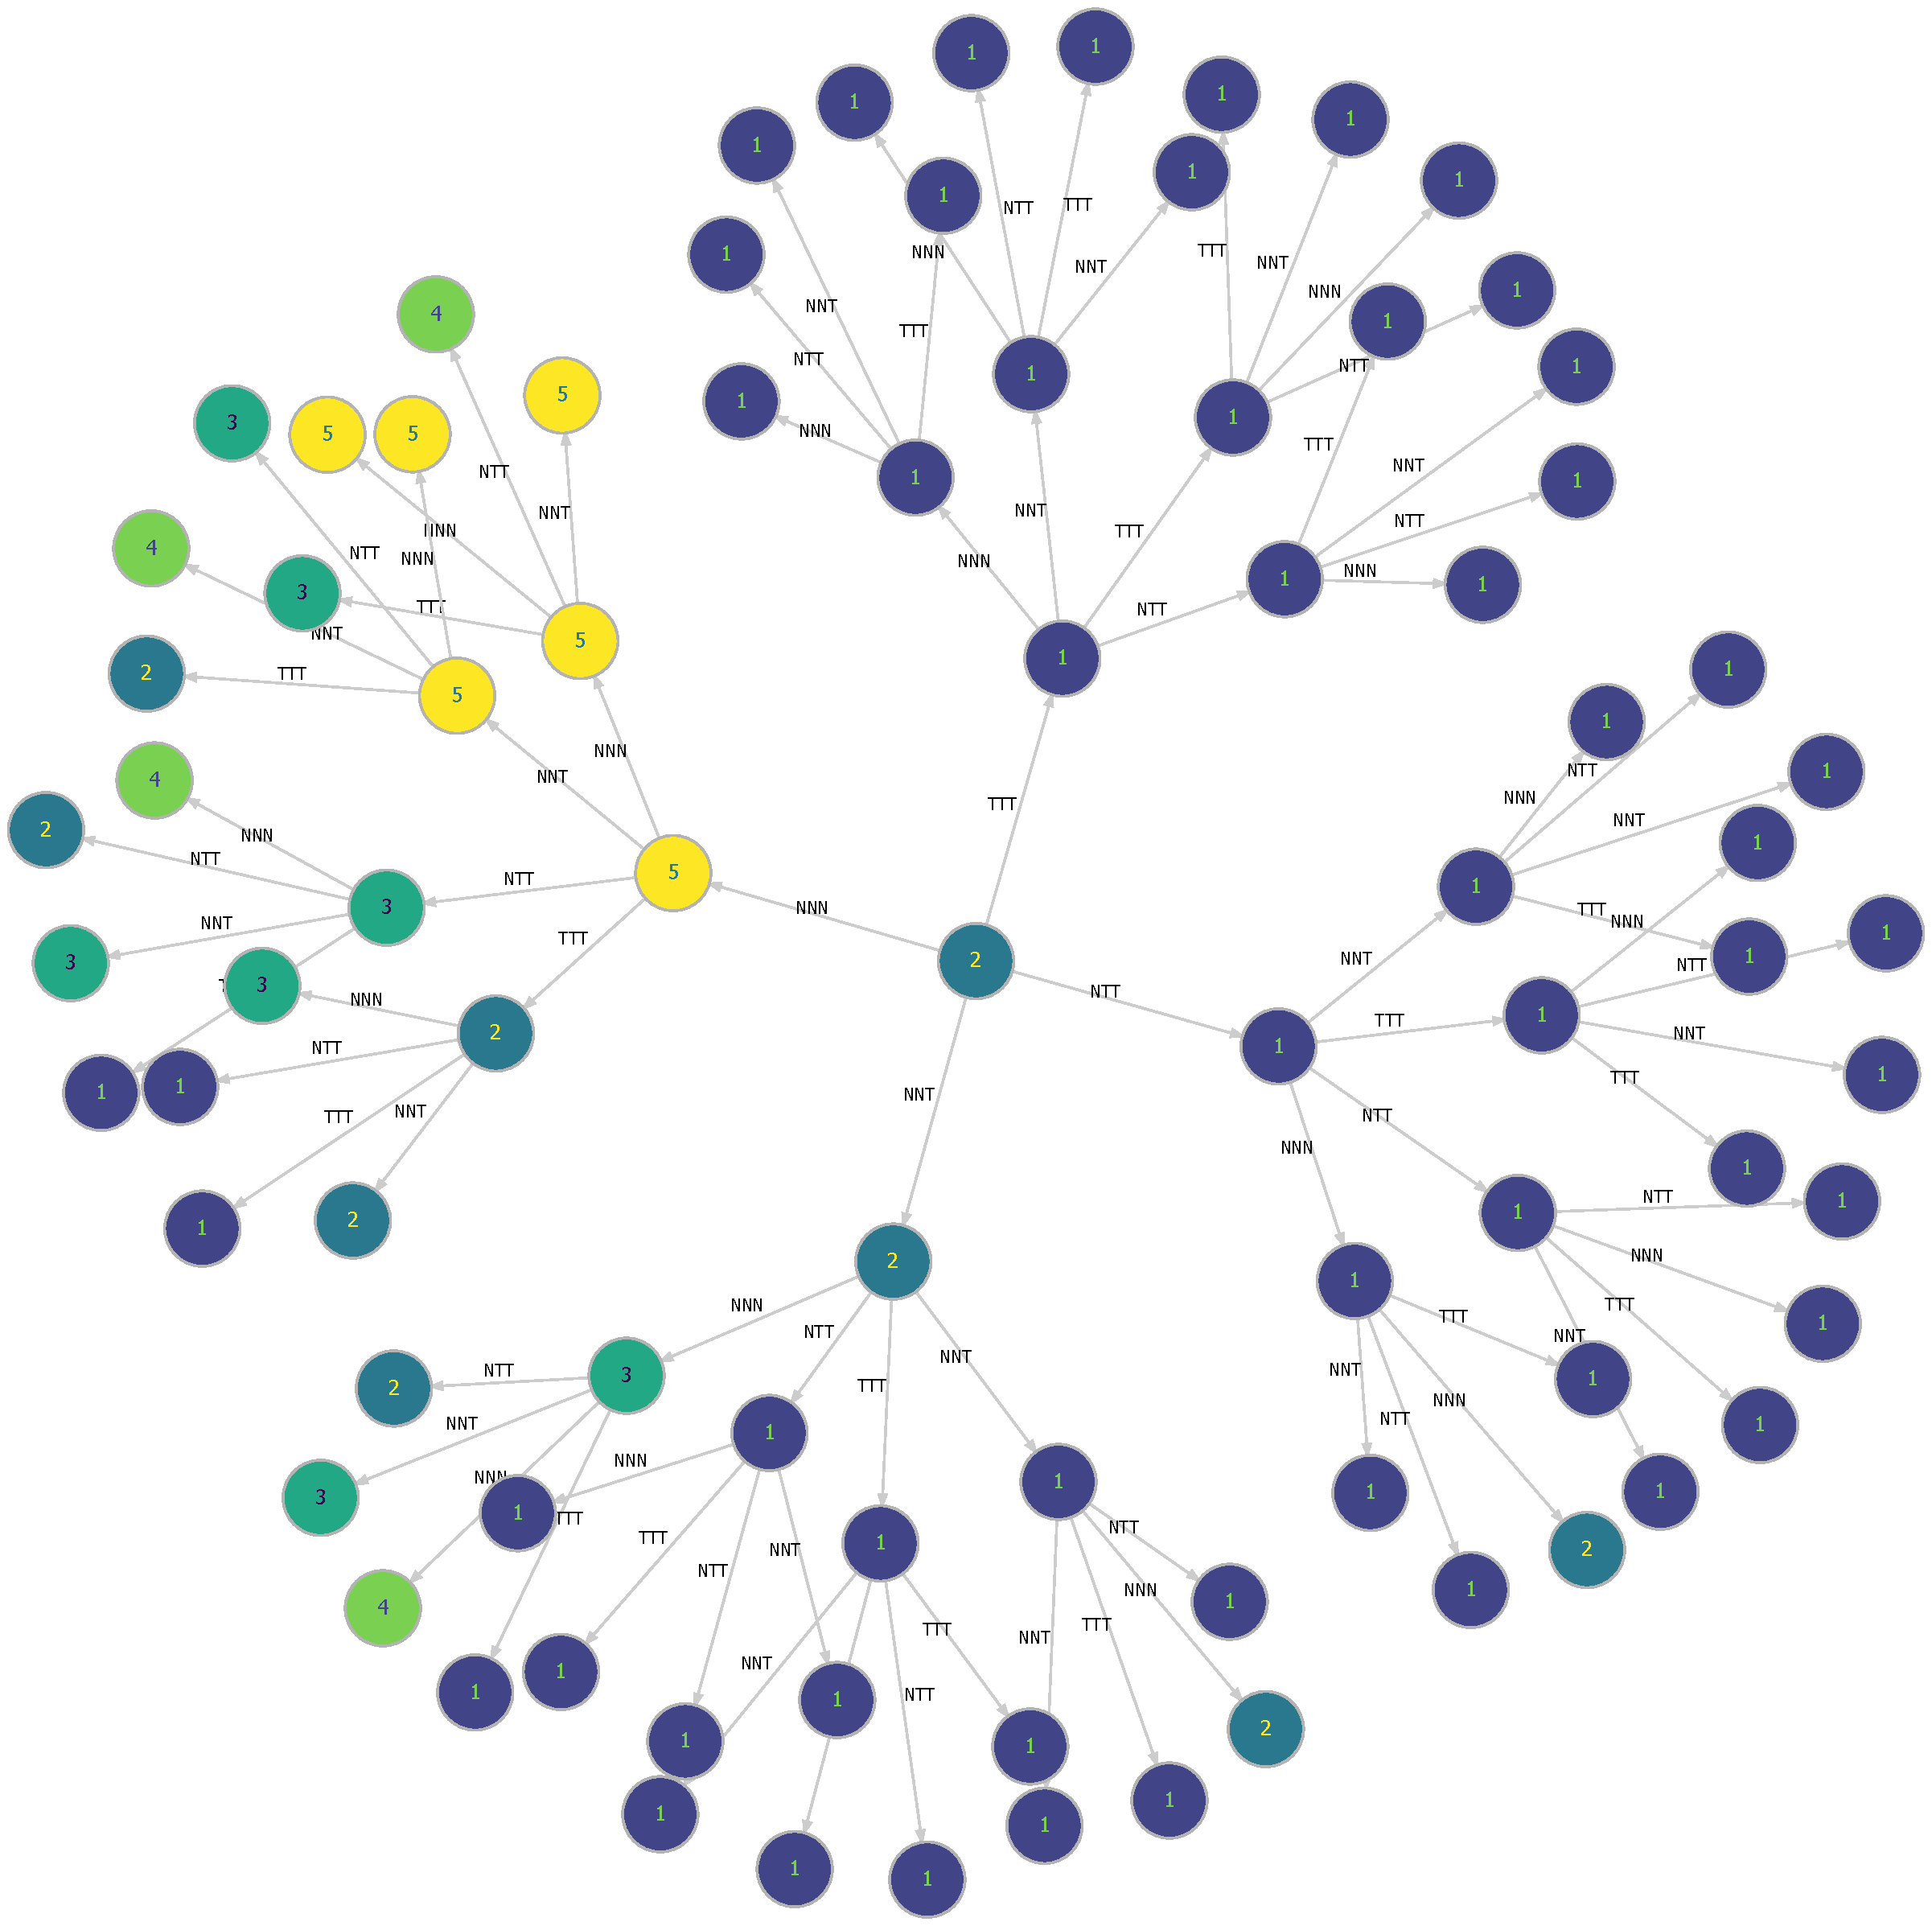
\includegraphics[width=\textwidth]{TITE-DTP-InitialExampleDTPNode}
\end{figure}

\begin{figure}[h!]
	\centering
	\caption[Initial DTP flow plot.]{Flow plot of the initial DTP for the first two cohorts of our example CRM.}
	\label{fig_tite-dtp:InitialDTPExampleFlow}
	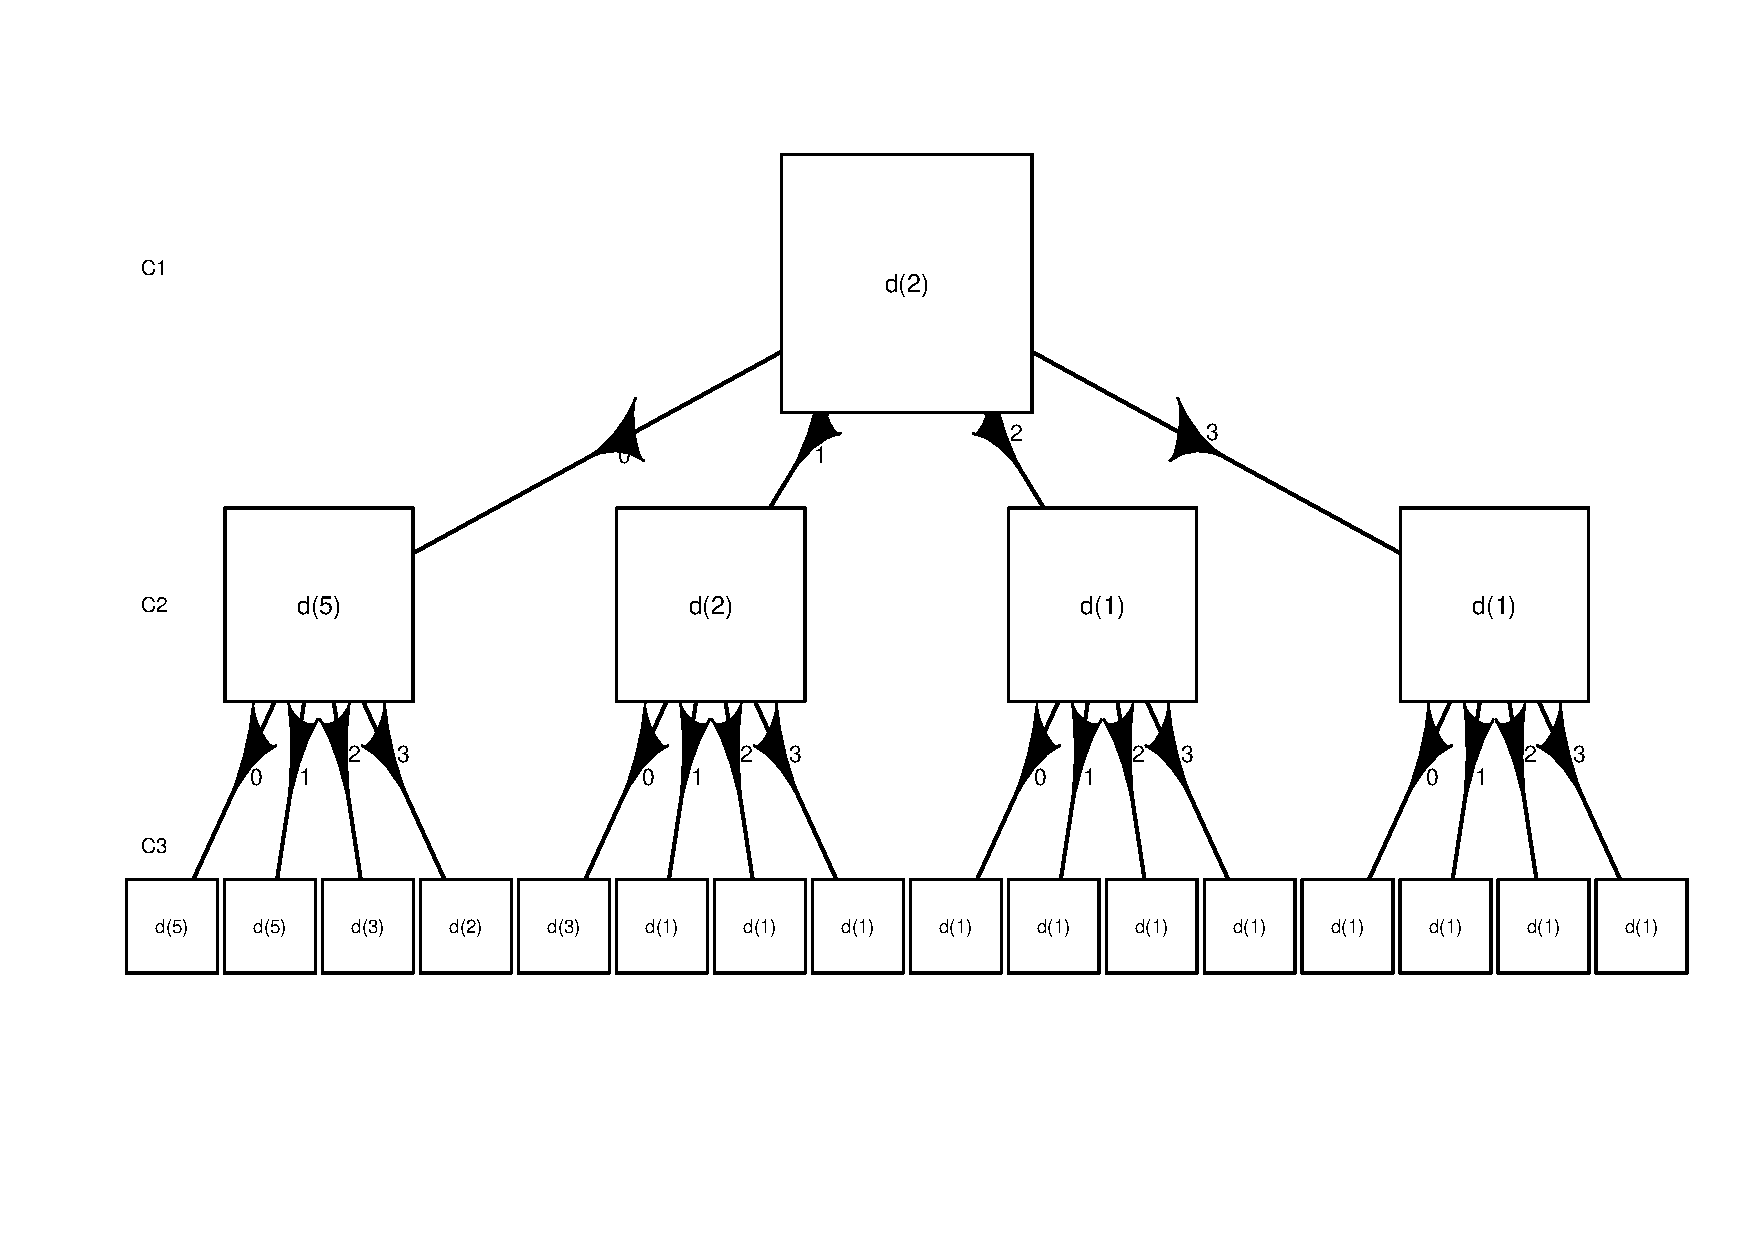
\includegraphics[width=\textwidth]{TITE-DTP-InitialExampleDTPFlow}
\end{figure}

From Table \ref{tab_tite-dtp:InitialDTPExample}, looking at pathways 33-64, we can see that if there are two or more toxicities in the first cohort the CRM will always de-escalate the dose and if there are one or more toxicities in the next two cohorts it will stay at dose-level 1. We can also see from pathways 17-32 that if we observe a toxicity event in the first cohort we will stay at the same dose-level for the next cohort. If no toxicities occur we escalate straight to the highest dose. 

Figure \ref{fig_tite-dtp:InitialDTPExampleNode} also shows the same information. The central node represents the starting dose and first cohort, from here we have 4 branches showing the various outcomes and which dose-level is allocated to the next cohort. In the case where each patient in the first cohort experience a DLT (TTT), we see that subsequent cohorts are all allocated to dose-level 1 regardless of their outcomes. Similarly, when two patients from the first cohort experience DLTs (NTT) all resulting branches show that dose-level 1 would be selected except in one case where no further DLTs occur and the CRM would escalate back to the starting dose. When one DLT occurs in the first cohort (NNT), we remain at the same dose-level. Looking at these branches if one or more DLTs are experienced in the next cohorts the dose-level is de-escalated, there is only potential for escalation in the scenario where no further DLTs occur. For the case when no DLTs occur (NNN) we see the dose for the second cohort escalated to dose-level 5. At this point, if the second cohort experiences 3 DLTs the CRM will de-escalate to dose-level 2. If there are only 2 DLTs the CRM goes to dose-level 3 and one or fewer DLTs and the next cohort will remain at dose-level 5. The flow plot, Figure \ref{fig_tite-dtp:InitialDTPExampleFlow}, only shows outcomes up to the third cohort but can be interpreted similarly to the node plot.

In combination with operating characteristics from simulations, DTPs can be used to facilitate discussions to see if the CRM can be better calibrated and is behaving optimally. In our example here there may be a few obvious things that would concern clinicians, the first being that we skip doses when escalating and the second that in the cases where lots of toxicity occurs recruitment continues. To remedy this we can include a rule to not skip untried doses and add a safety rule to stop the trial if too many toxicities occur at the lowest dose. 

In a Bayesian setting, an appropriate method to stop early would be to test the posterior distribution for the probability of toxicity. For our example here we will stop if there is at least a 90\% probability that the toxicity rate is 10\% greater than the target level at the lowest dose. This can be expressed as $P($true DLT rate at $d_1 > 0.25 + 0.1$ | observed data and prior information $) > 0.9$. With the addition of these two rules we now have a modified CRM design. Again, for reference, updated simulations are provided in Table \ref{tab_tite-dtp:UpdatedCRMsimsexample}. The same scenarios as presented in Table \ref{tab_tite-dtp:InitialCRMsimsexample} were used to evaluate this new modified CRM. 

\begin{table}[H]
	
	\caption{\label{tab_tite-dtp:UpdatedCRMsimsexample}Updated selection probabilities from 10000 simulated trials under various scenarios for the example CRM with additional rules.}
	\centering
	\begin{tabular}[t]{cccccccc}
		\toprule
		\multicolumn{2}{c}{ } & \multicolumn{5}{c}{Dose Levels} \\
		\cmidrule(l{3pt}r{3pt}){3-7}
		&   & 1 & 2 & 3 & 4 & 5 & Stop\\
		\midrule
		Scenario & Prior DLT & 0.04 & 0.08 & 0.16 & 0.25 & 0.35 & \\
		\cmidrule{1-8}
		& True DLT rate & 0.25 & 0.35 & 0.45 & 0.55 & 0.65 & \\
		
		\multirow{-2}{*}{\centering\arraybackslash 1:TD25 @1} & P(Select) & 0.66 & 0.26 & 0.05 & 0 & 0 & 0.02\\
		\cmidrule{1-8}
		& True DLT rate & 0.15 & 0.25 & 0.35 & 0.45 & 0.55 & \\
		
		\multirow{-2}{*}{\centering\arraybackslash 2:TD25 @2} & P(Select) & 0.23 & 0.47 & 0.25 & 0.04 & 0 & 0\\
		\cmidrule{1-8}
		& True DLT rate & 0.1 & 0.15 & 0.25 & 0.35 & 0.45 & \\
		
		\multirow{-2}{*}{\centering\arraybackslash 3:TD25 @3} & P(Select) & 0.03 & 0.21 & 0.48 & 0.24 & 0.04 & 0\\
		\cmidrule{1-8}
		& True DLT rate & 0.05 & 0.1 & 0.15 & 0.25 & 0.35 & \\
		
		\multirow{-2}{*}{\centering\arraybackslash 4:TD25 @4} & P(Select) & 0 & 0.03 & 0.25 & 0.46 & 0.26 & 0\\
		\cmidrule{1-8}
		& True DLT rate & 0.01 & 0.05 & 0.1 & 0.15 & 0.25 & \\
		
		\multirow{-2}{*}{\centering\arraybackslash 5:TD25 @5} & P(Select) & 0 & 0 & 0.04 & 0.26 & 0.71 & 0\\
		\cmidrule{1-8}
		& True DLT rate & 0.5 & 0.55 & 0.65 & 0.75 & 0.85 & \\
		
		\multirow{-2}{*}{\centering\arraybackslash 6:All toxic} & P(Select) & 0.34 & 0 & 0 & 0 & 0 & 0.66\\
		\bottomrule
	\end{tabular}
\end{table}

So, now along with our new simulation results DTPs can also be updated. Table \ref{tab_tite-dtp:UpdatedDTPExample} shows the pathways for the first three cohorts. The node and flow plots were also updated, Figures \ref{fig_tite-dtp:UpdatedDTPExampleNode} and \ref{fig_tite-dtp:UpdatedDTPExampleFlow} respectively. Since we included a rule to stop in the case of excess toxicity we see several pathways terminate early so overall there are fewer pathways compared to the initial set that was produced. Here we see six different branches where it recommended that the trial stop early (pathways 32, 44, 45, 53, 54, 55 Table \ref{tab_tite-dtp:UpdatedDTPExample}). This can also be seen in Figure \ref{fig_tite-dtp:UpdatedDTPExampleNode}, we can also see three of these nodes recommend stopping before recruiting a third cohort. Using the flow plot, in Figure \ref{fig_tite-dtp:UpdatedDTPExampleFlow}, we can see that stopping is suggested when five out of the first six patients experience a DLT. Also, escalation of doses no longer skips dose-levels. With these new rules, we observe that if there are no DLTs in the first cohort the dose for the next cohort is dose-level 3 and not 5. We still observe that one toxicity in the first cohort leads to recruiting the next cohort at that same dose-level and with two or more toxicities de-escalation occurs. 

\begin{table}[h!]
	
	\caption{\label{tab_tite-dtp:UpdatedDTPExample}Updated DTPs for the first three cohorts of our example CRM with additional rules.}
	\centering
	\resizebox{\linewidth}{!}{
		\fontsize{4}{3}\selectfont
		\begin{tabular}[t]{cccccccc}
			\toprule
			\multicolumn{1}{c}{} & \multicolumn{2}{c}{Cohort 1} & \multicolumn{2}{c}{Cohort 2} & \multicolumn{2}{c}{Cohort 3} & \multicolumn{1}{c}{Cohort 4} \\
			\cmidrule(l{3pt}r{3pt}){2-3} \cmidrule(l{3pt}r{3pt}){4-5} \cmidrule(l{3pt}r{3pt}){6-7} \cmidrule(l{3pt}r{3pt}){8-8}
			Pathway & Dose & Outcomes & Dose & Outcomes & Dose & Outcomes & Dose\\
			\midrule
			\cellcolor{gray!6}{1} & \cellcolor{gray!6}{2} & \cellcolor{gray!6}{NNN} & \cellcolor{gray!6}{3} & \cellcolor{gray!6}{NNN} & \cellcolor{gray!6}{4} & \cellcolor{gray!6}{NNN} & \cellcolor{gray!6}{5}\\
			2 & 2 & NNN & 3 & NNN & 4 & NNT & 5\\
			\cellcolor{gray!6}{3} & \cellcolor{gray!6}{2} & \cellcolor{gray!6}{NNN} & \cellcolor{gray!6}{3} & \cellcolor{gray!6}{NNN} & \cellcolor{gray!6}{4} & \cellcolor{gray!6}{NTT} & \cellcolor{gray!6}{4}\\
			4 & 2 & NNN & 3 & NNN & 4 & TTT & 3\\
			\cellcolor{gray!6}{5} & \cellcolor{gray!6}{2} & \cellcolor{gray!6}{NNN} & \cellcolor{gray!6}{3} & \cellcolor{gray!6}{NNT} & \cellcolor{gray!6}{3} & \cellcolor{gray!6}{NNN} & \cellcolor{gray!6}{4}\\
			6 & 2 & NNN & 3 & NNT & 3 & NNT & 3\\
			\cellcolor{gray!6}{7} & \cellcolor{gray!6}{2} & \cellcolor{gray!6}{NNN} & \cellcolor{gray!6}{3} & \cellcolor{gray!6}{NNT} & \cellcolor{gray!6}{3} & \cellcolor{gray!6}{NTT} & \cellcolor{gray!6}{2}\\
			8 & 2 & NNN & 3 & NNT & 3 & TTT & 1\\
			\cellcolor{gray!6}{9} & \cellcolor{gray!6}{2} & \cellcolor{gray!6}{NNN} & \cellcolor{gray!6}{3} & \cellcolor{gray!6}{NTT} & \cellcolor{gray!6}{2} & \cellcolor{gray!6}{NNN} & \cellcolor{gray!6}{3}\\
			10 & 2 & NNN & 3 & NTT & 2 & NNT & 2\\
			\cellcolor{gray!6}{11} & \cellcolor{gray!6}{2} & \cellcolor{gray!6}{NNN} & \cellcolor{gray!6}{3} & \cellcolor{gray!6}{NTT} & \cellcolor{gray!6}{2} & \cellcolor{gray!6}{NTT} & \cellcolor{gray!6}{1}\\
			12 & 2 & NNN & 3 & NTT & 2 & TTT & 1\\
			\cellcolor{gray!6}{13} & \cellcolor{gray!6}{2} & \cellcolor{gray!6}{NNN} & \cellcolor{gray!6}{3} & \cellcolor{gray!6}{TTT} & \cellcolor{gray!6}{1} & \cellcolor{gray!6}{NNN} & \cellcolor{gray!6}{2}\\
			14 & 2 & NNN & 3 & TTT & 1 & NNT & 1\\
			\cellcolor{gray!6}{15} & \cellcolor{gray!6}{2} & \cellcolor{gray!6}{NNN} & \cellcolor{gray!6}{3} & \cellcolor{gray!6}{TTT} & \cellcolor{gray!6}{1} & \cellcolor{gray!6}{NTT} & \cellcolor{gray!6}{1}\\
			16 & 2 & NNN & 3 & TTT & 1 & TTT & 1\\
			\cellcolor{gray!6}{17} & \cellcolor{gray!6}{2} & \cellcolor{gray!6}{NNT} & \cellcolor{gray!6}{2} & \cellcolor{gray!6}{NNN} & \cellcolor{gray!6}{3} & \cellcolor{gray!6}{NNN} & \cellcolor{gray!6}{4}\\
			18 & 2 & NNT & 2 & NNN & 3 & NNT & 3\\
			\cellcolor{gray!6}{19} & \cellcolor{gray!6}{2} & \cellcolor{gray!6}{NNT} & \cellcolor{gray!6}{2} & \cellcolor{gray!6}{NNN} & \cellcolor{gray!6}{3} & \cellcolor{gray!6}{NTT} & \cellcolor{gray!6}{2}\\
			20 & 2 & NNT & 2 & NNN & 3 & TTT & 1\\
			\cellcolor{gray!6}{21} & \cellcolor{gray!6}{2} & \cellcolor{gray!6}{NNT} & \cellcolor{gray!6}{2} & \cellcolor{gray!6}{NNT} & \cellcolor{gray!6}{1} & \cellcolor{gray!6}{NNN} & \cellcolor{gray!6}{2}\\
			22 & 2 & NNT & 2 & NNT & 1 & NNT & 1\\
			\cellcolor{gray!6}{23} & \cellcolor{gray!6}{2} & \cellcolor{gray!6}{NNT} & \cellcolor{gray!6}{2} & \cellcolor{gray!6}{NNT} & \cellcolor{gray!6}{1} & \cellcolor{gray!6}{NTT} & \cellcolor{gray!6}{1}\\
			24 & 2 & NNT & 2 & NNT & 1 & TTT & 1\\
			\cellcolor{gray!6}{25} & \cellcolor{gray!6}{2} & \cellcolor{gray!6}{NNT} & \cellcolor{gray!6}{2} & \cellcolor{gray!6}{NTT} & \cellcolor{gray!6}{1} & \cellcolor{gray!6}{NNN} & \cellcolor{gray!6}{1}\\
			26 & 2 & NNT & 2 & NTT & 1 & NNT & 1\\
			\cellcolor{gray!6}{27} & \cellcolor{gray!6}{2} & \cellcolor{gray!6}{NNT} & \cellcolor{gray!6}{2} & \cellcolor{gray!6}{NTT} & \cellcolor{gray!6}{1} & \cellcolor{gray!6}{NTT} & \cellcolor{gray!6}{1}\\
			28 & 2 & NNT & 2 & NTT & 1 & TTT & 1\\
			\cellcolor{gray!6}{29} & \cellcolor{gray!6}{2} & \cellcolor{gray!6}{NNT} & \cellcolor{gray!6}{2} & \cellcolor{gray!6}{TTT} & \cellcolor{gray!6}{1} & \cellcolor{gray!6}{NNN} & \cellcolor{gray!6}{1}\\
			30 & 2 & NNT & 2 & TTT & 1 & NNT & 1\\
			\cellcolor{gray!6}{31} & \cellcolor{gray!6}{2} & \cellcolor{gray!6}{NNT} & \cellcolor{gray!6}{2} & \cellcolor{gray!6}{TTT} & \cellcolor{gray!6}{1} & \cellcolor{gray!6}{NTT} & \cellcolor{gray!6}{1}\\
			32 & 2 & NNT & 2 & TTT & 1 & TTT & STOP\\
			\cellcolor{gray!6}{33} & \cellcolor{gray!6}{2} & \cellcolor{gray!6}{NTT} & \cellcolor{gray!6}{1} & \cellcolor{gray!6}{NNN} & \cellcolor{gray!6}{1} & \cellcolor{gray!6}{NNN} & \cellcolor{gray!6}{2}\\
			34 & 2 & NTT & 1 & NNN & 1 & NNT & 1\\
			\cellcolor{gray!6}{35} & \cellcolor{gray!6}{2} & \cellcolor{gray!6}{NTT} & \cellcolor{gray!6}{1} & \cellcolor{gray!6}{NNN} & \cellcolor{gray!6}{1} & \cellcolor{gray!6}{NTT} & \cellcolor{gray!6}{1}\\
			36 & 2 & NTT & 1 & NNN & 1 & TTT & 1\\
			\cellcolor{gray!6}{37} & \cellcolor{gray!6}{2} & \cellcolor{gray!6}{NTT} & \cellcolor{gray!6}{1} & \cellcolor{gray!6}{NNT} & \cellcolor{gray!6}{1} & \cellcolor{gray!6}{NNN} & \cellcolor{gray!6}{1}\\
			38 & 2 & NTT & 1 & NNT & 1 & NNT & 1\\
			\cellcolor{gray!6}{39} & \cellcolor{gray!6}{2} & \cellcolor{gray!6}{NTT} & \cellcolor{gray!6}{1} & \cellcolor{gray!6}{NNT} & \cellcolor{gray!6}{1} & \cellcolor{gray!6}{NTT} & \cellcolor{gray!6}{1}\\
			40 & 2 & NTT & 1 & NNT & 1 & TTT & 1\\
			\cellcolor{gray!6}{41} & \cellcolor{gray!6}{2} & \cellcolor{gray!6}{NTT} & \cellcolor{gray!6}{1} & \cellcolor{gray!6}{NTT} & \cellcolor{gray!6}{1} & \cellcolor{gray!6}{NNN} & \cellcolor{gray!6}{1}\\
			42 & 2 & NTT & 1 & NTT & 1 & NNT & 1\\
			\cellcolor{gray!6}{43} & \cellcolor{gray!6}{2} & \cellcolor{gray!6}{NTT} & \cellcolor{gray!6}{1} & \cellcolor{gray!6}{NTT} & \cellcolor{gray!6}{1} & \cellcolor{gray!6}{NTT} & \cellcolor{gray!6}{1}\\
			44 & 2 & NTT & 1 & NTT & 1 & TTT & STOP\\
			\cellcolor{gray!6}{45} & \cellcolor{gray!6}{2} & \cellcolor{gray!6}{NTT} & \cellcolor{gray!6}{1} & \cellcolor{gray!6}{TTT} & \cellcolor{gray!6}{STOP} & \cellcolor{gray!6}{NA} & \cellcolor{gray!6}{STOP}\\
			46 & 2 & TTT & 1 & NNN & 1 & NNN & 1\\
			\cellcolor{gray!6}{47} & \cellcolor{gray!6}{2} & \cellcolor{gray!6}{TTT} & \cellcolor{gray!6}{1} & \cellcolor{gray!6}{NNN} & \cellcolor{gray!6}{1} & \cellcolor{gray!6}{NNT} & \cellcolor{gray!6}{1}\\
			48 & 2 & TTT & 1 & NNN & 1 & NTT & 1\\
			\cellcolor{gray!6}{49} & \cellcolor{gray!6}{2} & \cellcolor{gray!6}{TTT} & \cellcolor{gray!6}{1} & \cellcolor{gray!6}{NNN} & \cellcolor{gray!6}{1} & \cellcolor{gray!6}{TTT} & \cellcolor{gray!6}{1}\\
			50 & 2 & TTT & 1 & NNT & 1 & NNN & 1\\
			\cellcolor{gray!6}{51} & \cellcolor{gray!6}{2} & \cellcolor{gray!6}{TTT} & \cellcolor{gray!6}{1} & \cellcolor{gray!6}{NNT} & \cellcolor{gray!6}{1} & \cellcolor{gray!6}{NNT} & \cellcolor{gray!6}{1}\\
			52 & 2 & TTT & 1 & NNT & 1 & NTT & 1\\
			\cellcolor{gray!6}{53} & \cellcolor{gray!6}{2} & \cellcolor{gray!6}{TTT} & \cellcolor{gray!6}{1} & \cellcolor{gray!6}{NNT} & \cellcolor{gray!6}{1} & \cellcolor{gray!6}{TTT} & \cellcolor{gray!6}{STOP}\\
			54 & 2 & TTT & 1 & NTT & STOP & NA & STOP\\
			\cellcolor{gray!6}{55} & \cellcolor{gray!6}{2} & \cellcolor{gray!6}{TTT} & \cellcolor{gray!6}{1} & \cellcolor{gray!6}{TTT} & \cellcolor{gray!6}{STOP} & \cellcolor{gray!6}{NA} & \cellcolor{gray!6}{STOP}\\
			\bottomrule
	\end{tabular}}
\end{table}

\begin{figure}[h!]
	\centering
	\caption[Updated DTP node plot.]{Updated DTP node plot for the first three cohorts of our example CRM with additional rules.}
	\label{fig_tite-dtp:UpdatedDTPExampleNode}
	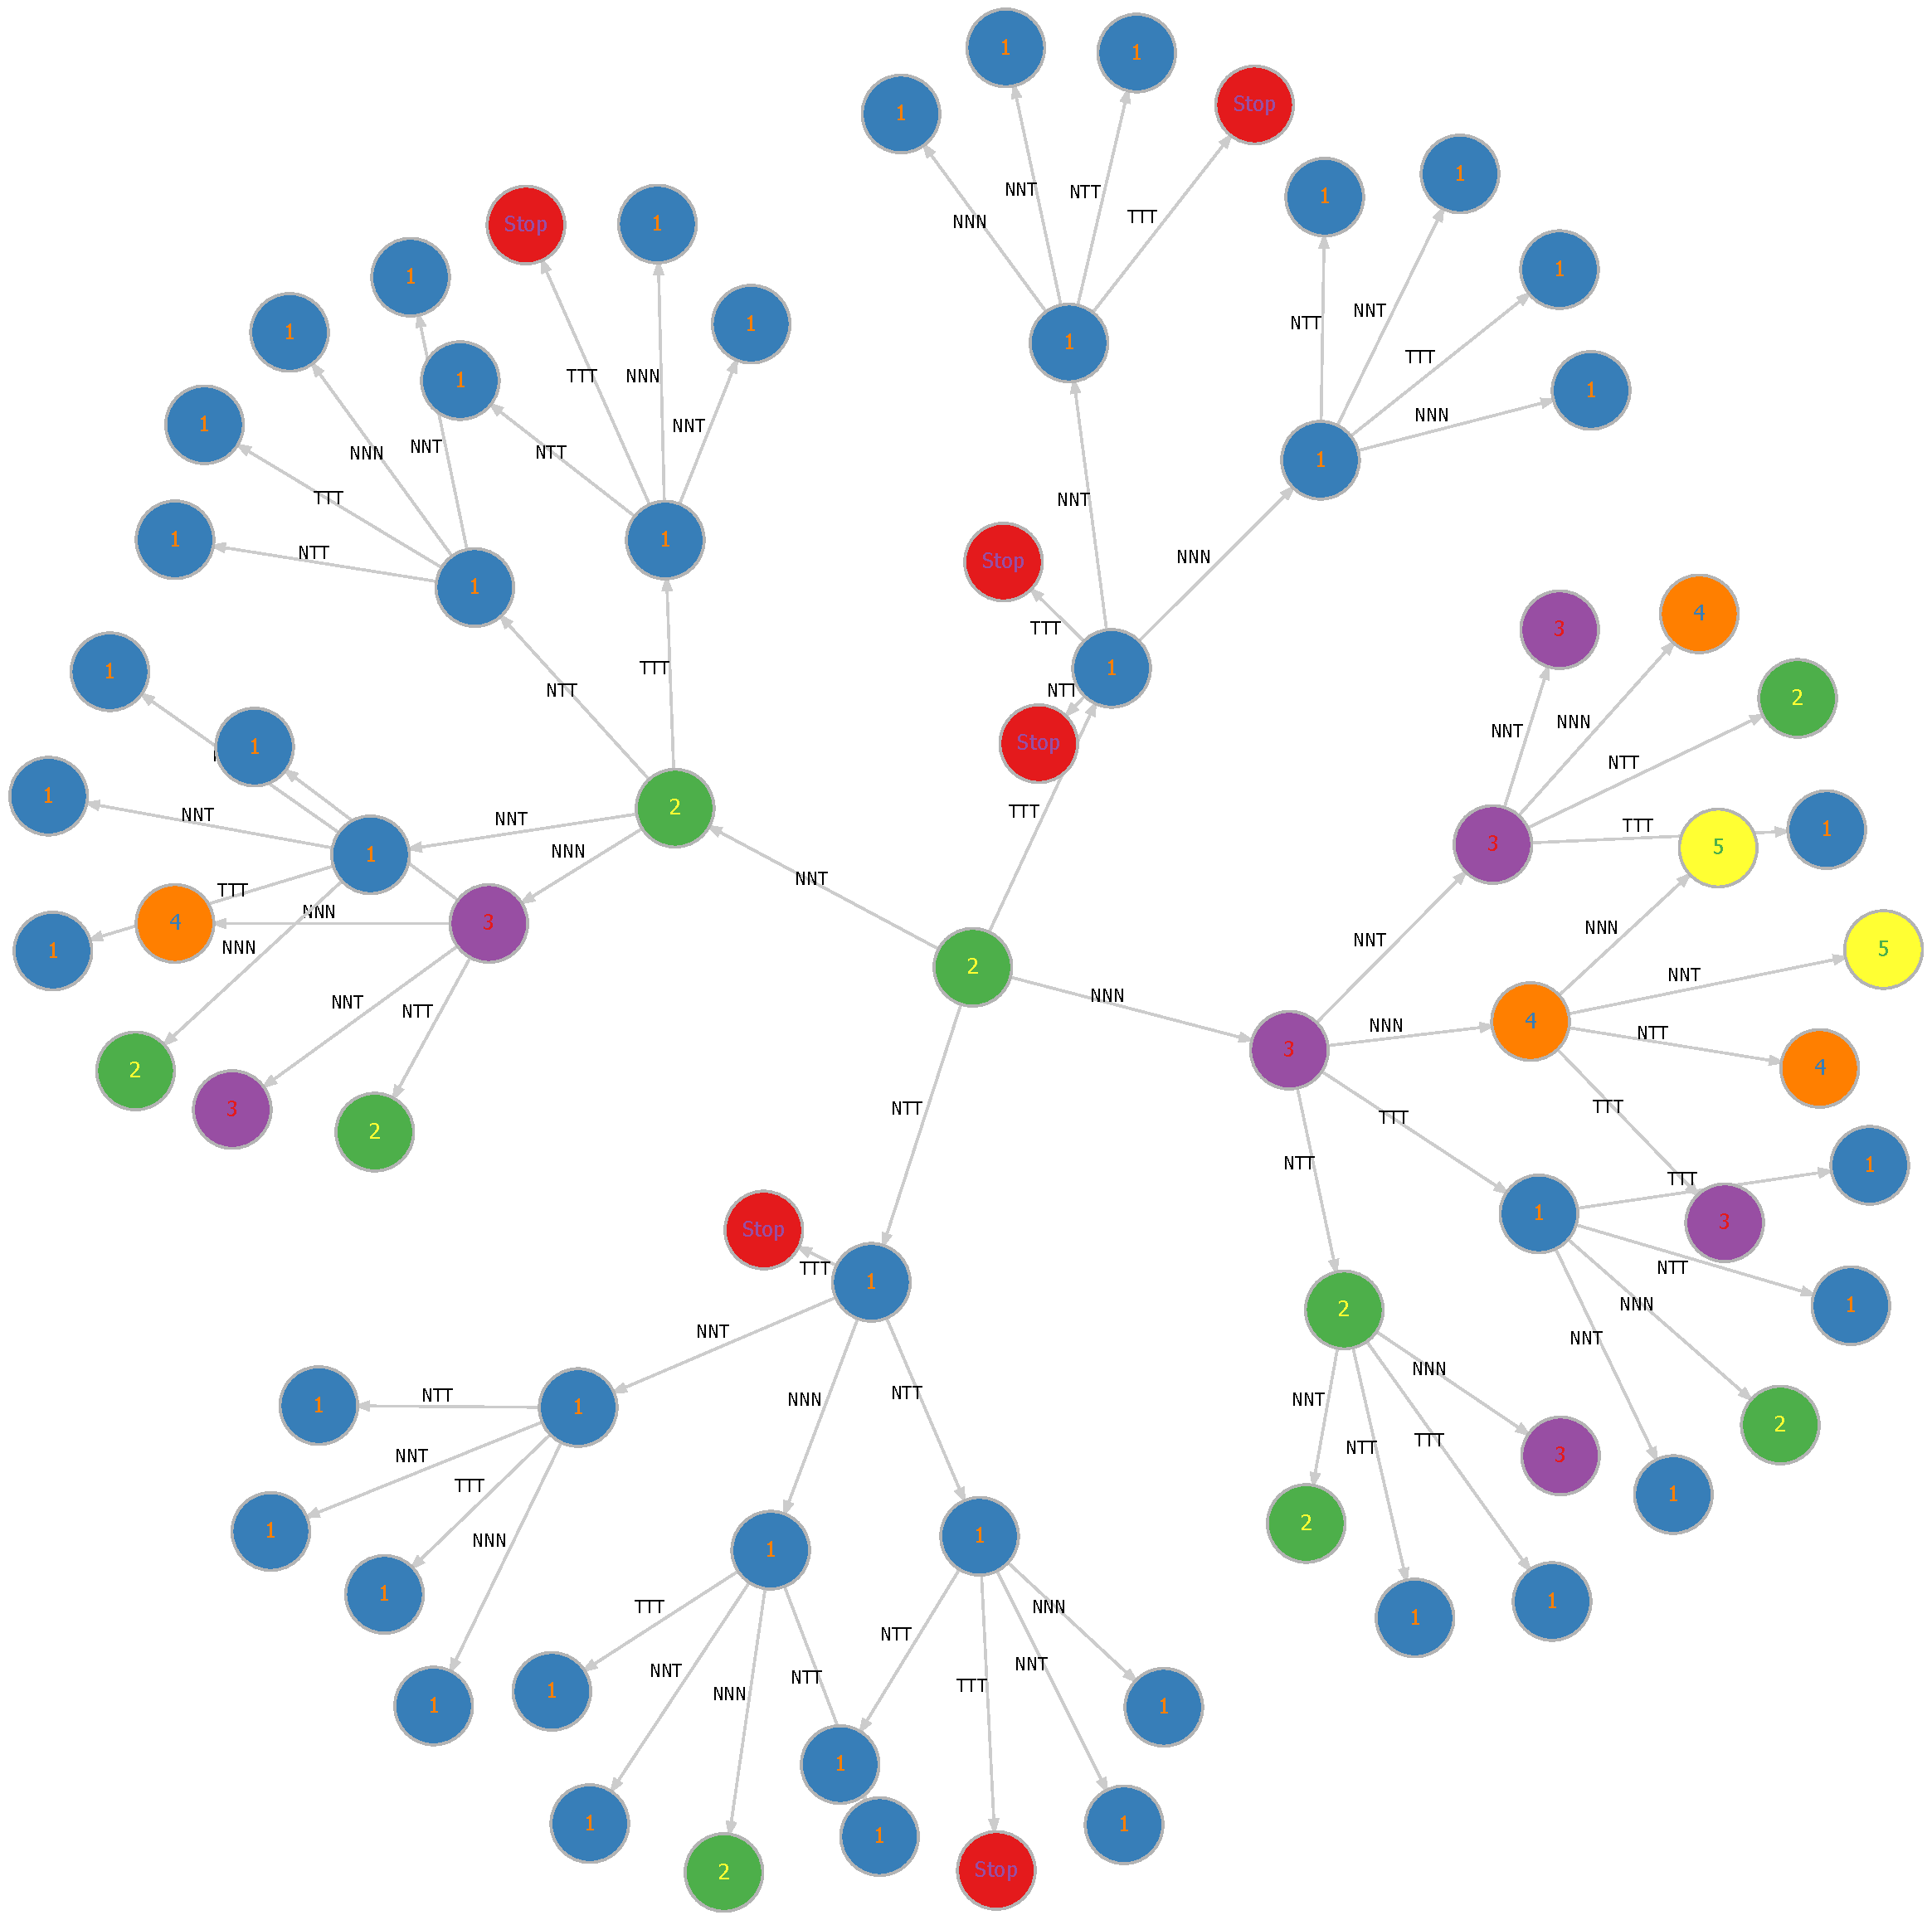
\includegraphics[width=\textwidth]{TITE-DTP-UpdatedExampleDTPNode}
\end{figure}

\begin{figure}[h!]
	\centering
	\caption[Updated DTP flow plot.]{Flow plot of the updated DTP for the first two cohorts of our example CRM with additional rules.}
	\label{fig_tite-dtp:UpdatedDTPExampleFlow}
	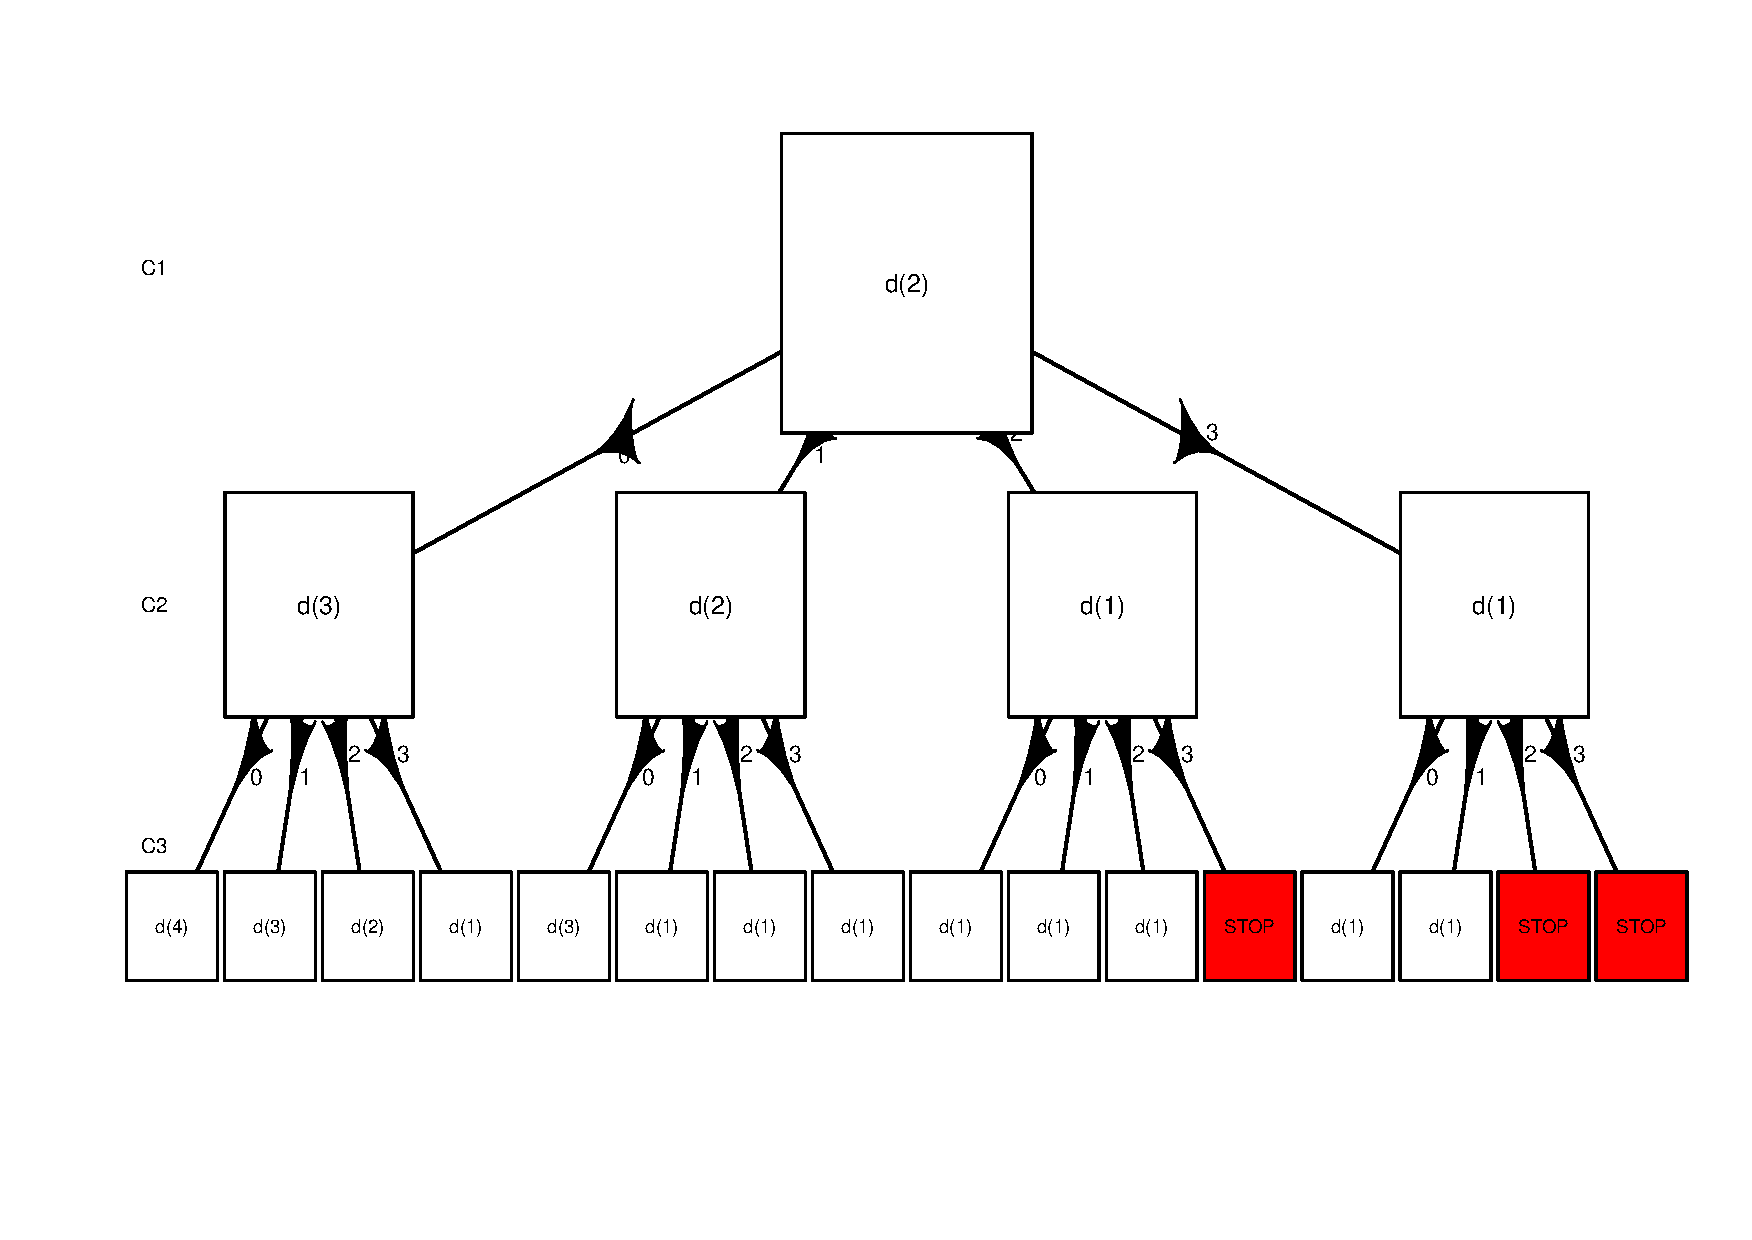
\includegraphics[width=\textwidth]{TITE-DTP-UpdatedExampleDTPFlow}
\end{figure}

At this stage, further discussions could be held about the updated DTPs and simulations. Here there may be more subtle points to discuss such as the parameters of the stopping rule. Dependent on the clinical rationale investigators may be inclined to impose either looser or stricter stopping rules. In our example, this can be done by altering the threshold values in our test of the posterior distribution of the probability of toxicity at the lowest dose. 

We also see in pathway 2 that an escalation occurs after observing a toxicity event in the previous cohort. This shows our design to be incoherent. A CRM design is considered coherent if escalation only occurs when the previous cohort experiences no DLTs and de-escalation only occurs when a DLT has been observed in the previous cohort. This property limits the risk of unnecessarily exposing patients to toxic doses whilst also ensuring patients get treated at a reasonable dose within the safety limit \cite{cheungDoseFindingContinual2011}. This became an issue due to the rule we enforced not to skip doses in escalation, the previous design without this rule was coherent. Further rules could be added to ensure the design remains coherent such that escalation will only take place if the previous cohort experience no DLTs likewise, de-escalation will only occur if the previous cohort did experience DLTs. 

We have mentioned how DTPs can be used in conjunction with operating characteristics from simulations to assist with the design of a trial. There is a further added benefit that probabilistic inference can be used with DTPs to ascertain exact operating characteristics of a design. This work was developed by Brock \cite{brockModularApproachDose2020} as part of the escalation package which he referred to as crystallised dose-paths. As we do with simulations for a specific scenario, if we specify an assumed truth about the toxicity probabilities at each dose we can calculate the likelihood of each dose-path according to that truth. From this we can then determine the probability of recommending each dose or stopping the trial. The benefits of calculating operating characteristics this way is that it can potentially be quicker than simulations. This is specifically true for smaller trials where if we were to run 10000 iterations for a trial with five cohorts of three patients that would require 50000 model fits. Whereas with crystallised dose-paths models only have to be fit once at each node which in this example corresponds to 1365 model fits. (There are four outcomes for a cohort of three patients NNN, NNT, NTT, TTT at each cohort the number of nodes will multiply by our number of outcomes. We start with one node which produces four outcomes equating to four more nodes. Each of those four nodes then has an additional four nodes for the next cohort. So, for five cohorts we go from one node to four to 16 to 256 to 1024. Summing all these values gives us the total number of nodes which is the total number of times the model would have to be fit). Even in instances where it may not be more efficient to produce these crystallised dose-paths they have the added benefit of not suffering from Monte Carlo error. There is no uncertainty associated with these exact probabilities but rather about which path will be taken based on outcomes observed. There are some inherent advantages that mean in practice it may be a better option to use dose-paths over simulations. 

Here we have highlighted how DTPs can be utilised during the initial stages of setting up a trial. Due to our example, some obvious changes could be implemented into our suggested design to improve it. However, this was just to illustrate what the pathways look like and how they can be used to facilitate discussions with the relevant clinicians and the trials team. Although we just looked at DTPs any changes being made to the design should also take into account operating characteristics from simulations or from crystallised dose-paths. CRM designs may not be intuitively understood by clinicians but DTPs should help make them more accessible. Next, we will look at how DTPs can be used during a trial.  
%-----------------------------------
%	SUBSECTION 2
%-----------------------------------

\subsection{Using DTPs during a trial}

Dependent on the size of the dose-finding trial it will often be infeasible to present all the different pathways. In our example with only 30 patients, there were approximately 1 million different pathways. As the trial progresses we observe outcomes for each patient and thus the number of pathways is reduced. This makes it possible to present DTPs for future cohorts of patients once we have accrued the outcome data of previous cohorts. 

DTPs main use in the design stage is allowing you to see how the model behaves with certain data generated by the earlier cohorts and we can see if escalation and stopping are occurring as expected. We can then also communicate more effectively with clinicians and investigators about what our design is doing. So, once a dose-finding trial has been designed, we can continue using DTPs whilst we are accruing data to project in advance dose decisions that may occur. This has the potential to reduce the involvement of a statistician in the running and operational side of the trial. Additionally, the time between the recruitment of cohorts could also be reduced if the next recommended dose is the same dose regardless of the outcomes observed in the current cohort. It also allows the statistician to check that the model is still escalating and stopping as expected. Although it may be more difficult to make changes to the design of the trial once it is underway. 

To see how this would work in practice we will use the same example as specified in Section \ref{tite-dtp:Example-DTPs} along with the stopping rule we introduced in Section \ref{tite-dtp:UsingDTPs-Calibration}. Essentially, the same design that was used to produce the DTPs in Table \ref{tab_tite-dtp:UpdatedDTPExample} and Figure \ref{fig_tite-dtp:UpdatedDTPExampleNode}. Let's assume that we run this trial and that we see outcomes for the first three cohorts that match pathway 6 in Table \ref{tab_tite-dtp:UpdatedDTPExample}. That's to say; the first cohort of patients is recruited to dose-level 2 and no toxicities are observed, cohort 2 is allocated to dose-level 3 where one toxicity is observed, then cohort 3 is allocated to dose-level 3 where again only one toxicity is observed and that leads the model recommending dose-level 3 for cohort 4. To refer to previous cohorts' outcomes we will use the nomenclature introduced by Brock \cite{brockImplementingEffToxDosefinding2017}. Outcomes for patients, either toxicity (T) or no toxicity (N) are strung behind a numeric dose-level. For instance, 2TTN denotes a cohort of three patients that were allocated to dose-level 2, two of whom experienced toxicity and one who did not. In our example, using pathway 6 from Table \ref{tab_tite-dtp:UpdatedDTPExample}, these outcomes can be denoted as 2NNN 3NNT 3NNT. In this scenario we are unsure about the toxicity of dose-level 3 as we have seen toxicities in two separate cohorts, however, this is mainly due to only having recruited three cohorts. If we consider this our new starting point we can produce new DTPs based on the observed data at that time. 

Table \ref{tab_tite-dtp:UsingDuringTrialDTPs4-7} shows the new set of DTPs following previous outcomes (2NNN 3NNT 3NNT), these are also visualised in Figure \ref{fig_tite-dtp:UsingDuringTrialDTPNode4-7}. For each pathway, cohort 4 patients start at dose-level 3 as this is the model recommendation based on the previously observed outcomes. We have 64 pathways again which indicates that regardless of how many toxicities are observed the trial does not recommend stopping. See pathway 64, three patients have a toxicity event at dose-level 3 and then six have toxicities at dose-level 1. This does not necessarily mean that the stopping rule is not working as intended rather due to the non-toxicities observed in the first three cohorts there would need to be more toxicity events before the rule we specified is triggered. This could be investigated further by looking at the DTPs following the outcomes of pathway 64 (i.e 2NNN 3NNT 3NNT 3TTT 1TTT 1TTT). 

It can also be seen if there are two in cohort 4 (pathways 33-48) we de-escalate to dose-level 2 and if there are three (pathways 49-64) we de-escalate to dose-level 1. If one toxicity occurs we stay at dose-level 3 (pathways 17-32). If no toxicities are observed we escalate to dose-level 4 (pathways 1-16). There are also only four pathways where we end up at a higher dose in cohort 7 (pathways 1, 2, 5 and 17). Given the data we have already observed and if another toxicity occurs in cohort 4 there would need to be two cohorts of no toxicities before escalation can take place (pathway 17). 


\begin{table}[H]
	
	\caption{\label{tab_tite-dtp:UsingDuringTrialDTPs4-7}DTPs for three additional cohorts after observing outcomes for the first three cohorts.}
	\centering
	\resizebox{\linewidth}{!}{
		\fontsize{4}{3}\selectfont
		\begin{tabular}[t]{cccccccc}
			\toprule
			\multicolumn{1}{c}{} & \multicolumn{2}{c}{Cohort 4} & \multicolumn{2}{c}{Cohort 5} & \multicolumn{2}{c}{Cohort 6} & \multicolumn{1}{c}{Cohort 7} \\
			\cmidrule(l{3pt}r{3pt}){2-3} \cmidrule(l{3pt}r{3pt}){4-5} \cmidrule(l{3pt}r{3pt}){6-7} \cmidrule(l{3pt}r{3pt}){8-8}
			Pathway & Dose & Outcomes & Dose & Outcomes & Dose & Outcomes & Dose\\
			\midrule
			\cellcolor{gray!6}{1} & \cellcolor{gray!6}{3} & \cellcolor{gray!6}{NNN} & \cellcolor{gray!6}{4} & \cellcolor{gray!6}{NNN} & \cellcolor{gray!6}{4} & \cellcolor{gray!6}{NNN} & \cellcolor{gray!6}{5}\\
			2 & 3 & NNN & 4 & NNN & 4 & NNT & 4\\
			\cellcolor{gray!6}{3} & \cellcolor{gray!6}{3} & \cellcolor{gray!6}{NNN} & \cellcolor{gray!6}{4} & \cellcolor{gray!6}{NNN} & \cellcolor{gray!6}{4} & \cellcolor{gray!6}{NTT} & \cellcolor{gray!6}{3}\\
			4 & 3 & NNN & 4 & NNN & 4 & TTT & 3\\
			\cellcolor{gray!6}{5} & \cellcolor{gray!6}{3} & \cellcolor{gray!6}{NNN} & \cellcolor{gray!6}{4} & \cellcolor{gray!6}{NNT} & \cellcolor{gray!6}{4} & \cellcolor{gray!6}{NNN} & \cellcolor{gray!6}{4}\\
			6 & 3 & NNN & 4 & NNT & 4 & NNT & 3\\
			\cellcolor{gray!6}{7} & \cellcolor{gray!6}{3} & \cellcolor{gray!6}{NNN} & \cellcolor{gray!6}{4} & \cellcolor{gray!6}{NNT} & \cellcolor{gray!6}{4} & \cellcolor{gray!6}{NTT} & \cellcolor{gray!6}{3}\\
			8 & 3 & NNN & 4 & NNT & 4 & TTT & 3\\
			\cellcolor{gray!6}{9} & \cellcolor{gray!6}{3} & \cellcolor{gray!6}{NNN} & \cellcolor{gray!6}{4} & \cellcolor{gray!6}{NTT} & \cellcolor{gray!6}{3} & \cellcolor{gray!6}{NNN} & \cellcolor{gray!6}{3}\\
			10 & 3 & NNN & 4 & NTT & 3 & NNT & 3\\
			\cellcolor{gray!6}{11} & \cellcolor{gray!6}{3} & \cellcolor{gray!6}{NNN} & \cellcolor{gray!6}{4} & \cellcolor{gray!6}{NTT} & \cellcolor{gray!6}{3} & \cellcolor{gray!6}{NTT} & \cellcolor{gray!6}{2}\\
			12 & 3 & NNN & 4 & NTT & 3 & TTT & 2\\
			\cellcolor{gray!6}{13} & \cellcolor{gray!6}{3} & \cellcolor{gray!6}{NNN} & \cellcolor{gray!6}{4} & \cellcolor{gray!6}{TTT} & \cellcolor{gray!6}{2} & \cellcolor{gray!6}{NNN} & \cellcolor{gray!6}{3}\\
			14 & 3 & NNN & 4 & TTT & 2 & NNT & 2\\
			\cellcolor{gray!6}{15} & \cellcolor{gray!6}{3} & \cellcolor{gray!6}{NNN} & \cellcolor{gray!6}{4} & \cellcolor{gray!6}{TTT} & \cellcolor{gray!6}{2} & \cellcolor{gray!6}{NTT} & \cellcolor{gray!6}{2}\\
			16 & 3 & NNN & 4 & TTT & 2 & TTT & 1\\
			\cellcolor{gray!6}{17} & \cellcolor{gray!6}{3} & \cellcolor{gray!6}{NNT} & \cellcolor{gray!6}{3} & \cellcolor{gray!6}{NNN} & \cellcolor{gray!6}{3} & \cellcolor{gray!6}{NNN} & \cellcolor{gray!6}{4}\\
			18 & 3 & NNT & 3 & NNN & 3 & NNT & 3\\
			\cellcolor{gray!6}{19} & \cellcolor{gray!6}{3} & \cellcolor{gray!6}{NNT} & \cellcolor{gray!6}{3} & \cellcolor{gray!6}{NNN} & \cellcolor{gray!6}{3} & \cellcolor{gray!6}{NTT} & \cellcolor{gray!6}{3}\\
			20 & 3 & NNT & 3 & NNN & 3 & TTT & 2\\
			\cellcolor{gray!6}{21} & \cellcolor{gray!6}{3} & \cellcolor{gray!6}{NNT} & \cellcolor{gray!6}{3} & \cellcolor{gray!6}{NNT} & \cellcolor{gray!6}{3} & \cellcolor{gray!6}{NNN} & \cellcolor{gray!6}{3}\\
			22 & 3 & NNT & 3 & NNT & 3 & NNT & 3\\
			\cellcolor{gray!6}{23} & \cellcolor{gray!6}{3} & \cellcolor{gray!6}{NNT} & \cellcolor{gray!6}{3} & \cellcolor{gray!6}{NNT} & \cellcolor{gray!6}{3} & \cellcolor{gray!6}{NTT} & \cellcolor{gray!6}{2}\\
			24 & 3 & NNT & 3 & NNT & 3 & TTT & 2\\
			\cellcolor{gray!6}{25} & \cellcolor{gray!6}{3} & \cellcolor{gray!6}{NNT} & \cellcolor{gray!6}{3} & \cellcolor{gray!6}{NTT} & \cellcolor{gray!6}{2} & \cellcolor{gray!6}{NNN} & \cellcolor{gray!6}{3}\\
			26 & 3 & NNT & 3 & NTT & 2 & NNT & 2\\
			\cellcolor{gray!6}{27} & \cellcolor{gray!6}{3} & \cellcolor{gray!6}{NNT} & \cellcolor{gray!6}{3} & \cellcolor{gray!6}{NTT} & \cellcolor{gray!6}{2} & \cellcolor{gray!6}{NTT} & \cellcolor{gray!6}{1}\\
			28 & 3 & NNT & 3 & NTT & 2 & TTT & 1\\
			\cellcolor{gray!6}{29} & \cellcolor{gray!6}{3} & \cellcolor{gray!6}{NNT} & \cellcolor{gray!6}{3} & \cellcolor{gray!6}{TTT} & \cellcolor{gray!6}{2} & \cellcolor{gray!6}{NNN} & \cellcolor{gray!6}{2}\\
			30 & 3 & NNT & 3 & TTT & 2 & NNT & 1\\
			\cellcolor{gray!6}{31} & \cellcolor{gray!6}{3} & \cellcolor{gray!6}{NNT} & \cellcolor{gray!6}{3} & \cellcolor{gray!6}{TTT} & \cellcolor{gray!6}{2} & \cellcolor{gray!6}{NTT} & \cellcolor{gray!6}{1}\\
			32 & 3 & NNT & 3 & TTT & 2 & TTT & 1\\
			\cellcolor{gray!6}{33} & \cellcolor{gray!6}{3} & \cellcolor{gray!6}{NTT} & \cellcolor{gray!6}{2} & \cellcolor{gray!6}{NNN} & \cellcolor{gray!6}{3} & \cellcolor{gray!6}{NNN} & \cellcolor{gray!6}{3}\\
			34 & 3 & NTT & 2 & NNN & 3 & NNT & 3\\
			\cellcolor{gray!6}{35} & \cellcolor{gray!6}{3} & \cellcolor{gray!6}{NTT} & \cellcolor{gray!6}{2} & \cellcolor{gray!6}{NNN} & \cellcolor{gray!6}{3} & \cellcolor{gray!6}{NTT} & \cellcolor{gray!6}{2}\\
			36 & 3 & NTT & 2 & NNN & 3 & TTT & 2\\
			\cellcolor{gray!6}{37} & \cellcolor{gray!6}{3} & \cellcolor{gray!6}{NTT} & \cellcolor{gray!6}{2} & \cellcolor{gray!6}{NNT} & \cellcolor{gray!6}{2} & \cellcolor{gray!6}{NNN} & \cellcolor{gray!6}{2}\\
			38 & 3 & NTT & 2 & NNT & 2 & NNT & 2\\
			\cellcolor{gray!6}{39} & \cellcolor{gray!6}{3} & \cellcolor{gray!6}{NTT} & \cellcolor{gray!6}{2} & \cellcolor{gray!6}{NNT} & \cellcolor{gray!6}{2} & \cellcolor{gray!6}{NTT} & \cellcolor{gray!6}{1}\\
			40 & 3 & NTT & 2 & NNT & 2 & TTT & 1\\
			\cellcolor{gray!6}{41} & \cellcolor{gray!6}{3} & \cellcolor{gray!6}{NTT} & \cellcolor{gray!6}{2} & \cellcolor{gray!6}{NTT} & \cellcolor{gray!6}{1} & \cellcolor{gray!6}{NNN} & \cellcolor{gray!6}{2}\\
			42 & 3 & NTT & 2 & NTT & 1 & NNT & 1\\
			\cellcolor{gray!6}{43} & \cellcolor{gray!6}{3} & \cellcolor{gray!6}{NTT} & \cellcolor{gray!6}{2} & \cellcolor{gray!6}{NTT} & \cellcolor{gray!6}{1} & \cellcolor{gray!6}{NTT} & \cellcolor{gray!6}{1}\\
			44 & 3 & NTT & 2 & NTT & 1 & TTT & 1\\
			\cellcolor{gray!6}{45} & \cellcolor{gray!6}{3} & \cellcolor{gray!6}{NTT} & \cellcolor{gray!6}{2} & \cellcolor{gray!6}{TTT} & \cellcolor{gray!6}{1} & \cellcolor{gray!6}{NNN} & \cellcolor{gray!6}{1}\\
			46 & 3 & NTT & 2 & TTT & 1 & NNT & 1\\
			\cellcolor{gray!6}{47} & \cellcolor{gray!6}{3} & \cellcolor{gray!6}{NTT} & \cellcolor{gray!6}{2} & \cellcolor{gray!6}{TTT} & \cellcolor{gray!6}{1} & \cellcolor{gray!6}{NTT} & \cellcolor{gray!6}{1}\\
			48 & 3 & NTT & 2 & TTT & 1 & TTT & 1\\
			\cellcolor{gray!6}{49} & \cellcolor{gray!6}{3} & \cellcolor{gray!6}{TTT} & \cellcolor{gray!6}{1} & \cellcolor{gray!6}{NNN} & \cellcolor{gray!6}{2} & \cellcolor{gray!6}{NNN} & \cellcolor{gray!6}{2}\\
			50 & 3 & TTT & 1 & NNN & 2 & NNT & 2\\
			\cellcolor{gray!6}{51} & \cellcolor{gray!6}{3} & \cellcolor{gray!6}{TTT} & \cellcolor{gray!6}{1} & \cellcolor{gray!6}{NNN} & \cellcolor{gray!6}{2} & \cellcolor{gray!6}{NTT} & \cellcolor{gray!6}{1}\\
			52 & 3 & TTT & 1 & NNN & 2 & TTT & 1\\
			\cellcolor{gray!6}{53} & \cellcolor{gray!6}{3} & \cellcolor{gray!6}{TTT} & \cellcolor{gray!6}{1} & \cellcolor{gray!6}{NNT} & \cellcolor{gray!6}{1} & \cellcolor{gray!6}{NNN} & \cellcolor{gray!6}{2}\\
			54 & 3 & TTT & 1 & NNT & 1 & NNT & 1\\
			\cellcolor{gray!6}{55} & \cellcolor{gray!6}{3} & \cellcolor{gray!6}{TTT} & \cellcolor{gray!6}{1} & \cellcolor{gray!6}{NNT} & \cellcolor{gray!6}{1} & \cellcolor{gray!6}{NTT} & \cellcolor{gray!6}{1}\\
			56 & 3 & TTT & 1 & NNT & 1 & TTT & 1\\
			\cellcolor{gray!6}{57} & \cellcolor{gray!6}{3} & \cellcolor{gray!6}{TTT} & \cellcolor{gray!6}{1} & \cellcolor{gray!6}{NTT} & \cellcolor{gray!6}{1} & \cellcolor{gray!6}{NNN} & \cellcolor{gray!6}{1}\\
			58 & 3 & TTT & 1 & NTT & 1 & NNT & 1\\
			\cellcolor{gray!6}{59} & \cellcolor{gray!6}{3} & \cellcolor{gray!6}{TTT} & \cellcolor{gray!6}{1} & \cellcolor{gray!6}{NTT} & \cellcolor{gray!6}{1} & \cellcolor{gray!6}{NTT} & \cellcolor{gray!6}{1}\\
			60 & 3 & TTT & 1 & NTT & 1 & TTT & 1\\
			\cellcolor{gray!6}{61} & \cellcolor{gray!6}{3} & \cellcolor{gray!6}{TTT} & \cellcolor{gray!6}{1} & \cellcolor{gray!6}{TTT} & \cellcolor{gray!6}{1} & \cellcolor{gray!6}{NNN} & \cellcolor{gray!6}{1}\\
			62 & 3 & TTT & 1 & TTT & 1 & NNT & 1\\
			\cellcolor{gray!6}{63} & \cellcolor{gray!6}{3} & \cellcolor{gray!6}{TTT} & \cellcolor{gray!6}{1} & \cellcolor{gray!6}{TTT} & \cellcolor{gray!6}{1} & \cellcolor{gray!6}{NTT} & \cellcolor{gray!6}{1}\\
			64 & 3 & TTT & 1 & TTT & 1 & TTT & 1\\
			\bottomrule
	\end{tabular}}
\end{table}

\begin{figure}[h!]
	\centering
	\caption[DTP node plot for three additional cohorts.]{Node plot of three additional cohorts after observing outcomes for the first three cohorts.}
	\label{fig_tite-dtp:UsingDuringTrialDTPNode4-7}
	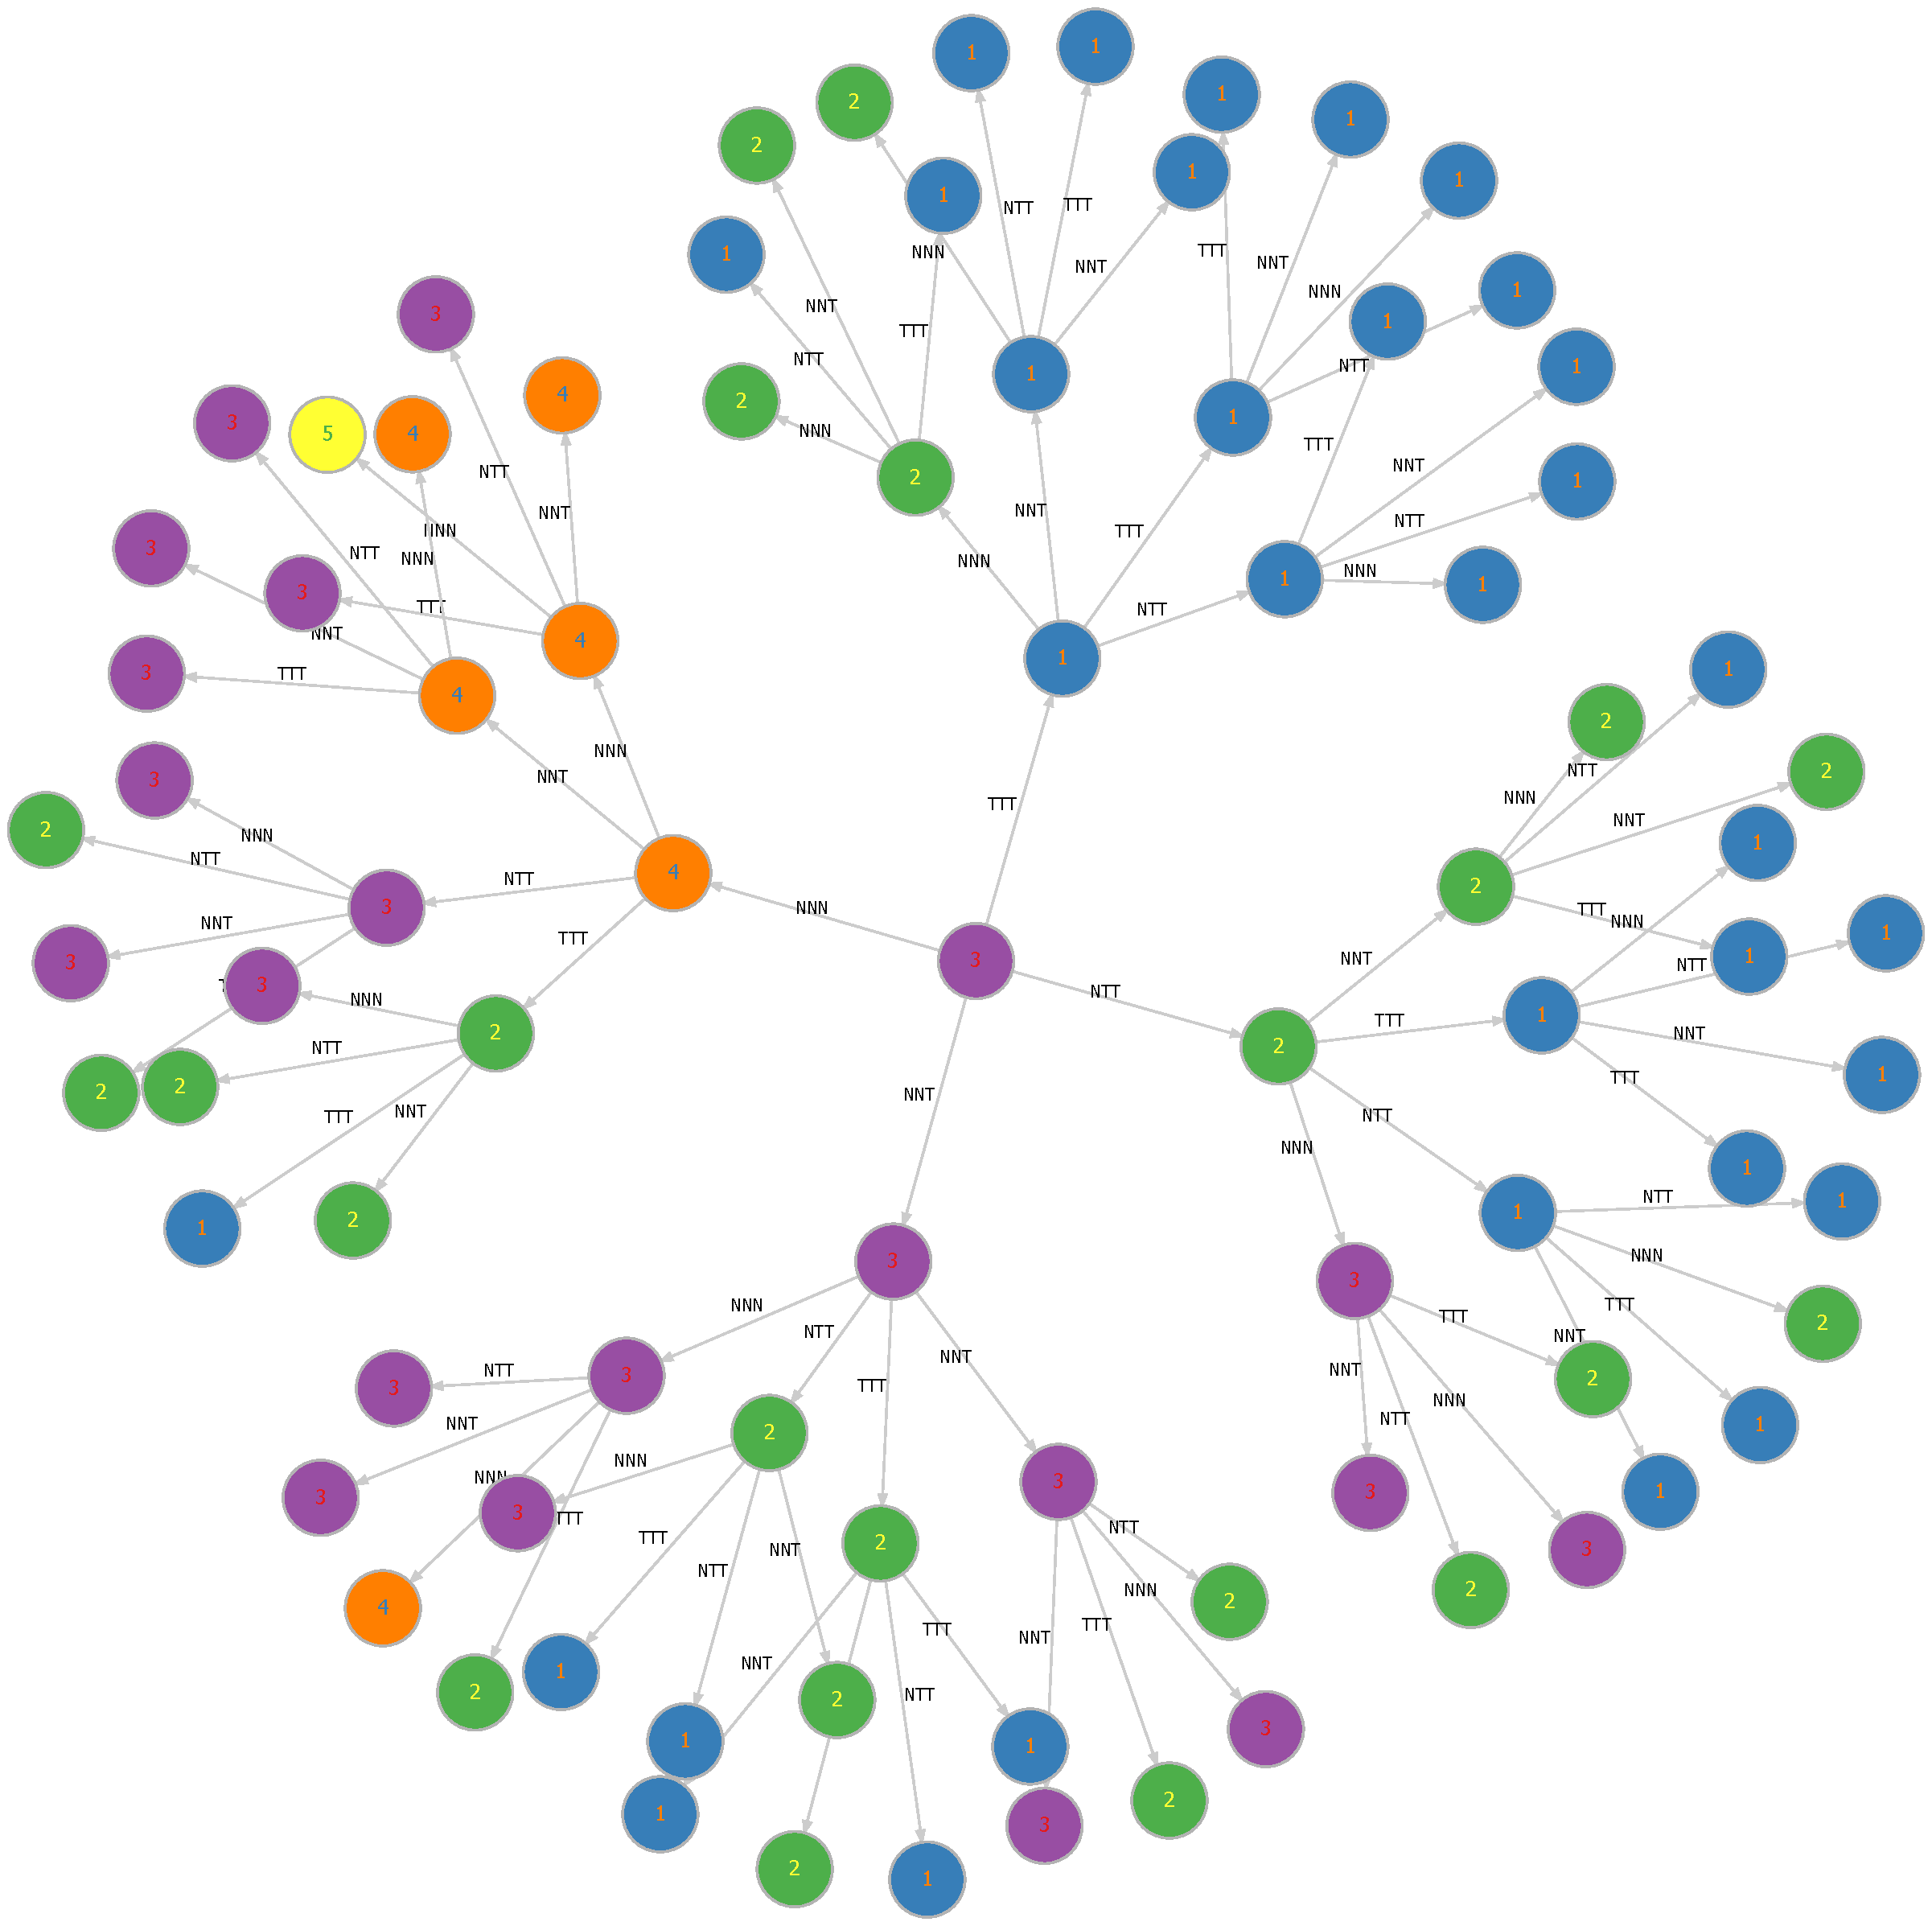
\includegraphics[width=\textwidth]{TITE-DTP-UsingDuringTrialDTPNode}
\end{figure}

Once cohort 7 is reached in the trial the DTPs can be updated again using the observed outcomes of whichever pathway occurred. These will show the potential pathways up to the 10th cohort, which is the maximum sample size in our example, and will also detail the final dose recommendation. Throughout the trial the DTPs allow us to map out what doses are recommended until the final decision. 

DTPs can also work with non-uniform cohorts. So far our examples have been fairly simple however, in practice there may be complications with running a dose-finding trial. For instance, there may be issues with recruitment leading to long time periods between the evaluation of cohorts and dose decisions. This may be due to a number of factors such as a lack of recruiting sites, underestimation of the prevalence of disease in the patient population, or a global pandemic. One solution to this may be to reduce the cohort size and make dose decisions earlier. Model-based designs are fairly flexible at dealing with issues like these as the model could just be updated after fewer patients instead. As these considerations may not have been made in the design stages of the trial, DTPs could be used as a way to evaluate any changes to cohort sizes that are made during the trial. 

We will recreate the DTPs presented earlier in this section except we will now use varying cohort sizes. These DTPs will use the same previously specified outcomes of 2NNN 3NNT 3NNT. DTPs will be calculated assuming the next three cohorts (cohorts 4,5 and 6) will only be able to recruit 2, 1 and 2 patients respectively. Table \ref{tab_tite-dtp:NonUniformDTPs4-7} lists the different pathways and they are also visualised in Figure \ref{fig_tite-dtp:NonUniformDTPNode4-7}. 

\begin{table}[H]
	
	\caption{\label{tab_tite-dtp:NonUniformDTPs4-7}DTPs for three additional cohorts with varying cohort sizes after observing outcomes for the first three cohorts.}
	\centering
	\resizebox{\linewidth}{!}{
		\fontsize{4}{3}\selectfont
		\begin{tabular}[t]{cccccccc}
			\toprule
			\multicolumn{1}{c}{} & \multicolumn{2}{c}{Cohort 4} & \multicolumn{2}{c}{Cohort 5} & \multicolumn{2}{c}{Cohort 6} & \multicolumn{1}{c}{Cohort 7} \\
			\cmidrule(l{3pt}r{3pt}){2-3} \cmidrule(l{3pt}r{3pt}){4-5} \cmidrule(l{3pt}r{3pt}){6-7} \cmidrule(l{3pt}r{3pt}){8-8}
			Pathway & Dose & Outcomes & Dose & Outcomes & Dose & Outcomes & Dose\\
			\midrule
			\cellcolor{gray!6}{1} & \cellcolor{gray!6}{3} & \cellcolor{gray!6}{NN} & \cellcolor{gray!6}{3} & \cellcolor{gray!6}{N} & \cellcolor{gray!6}{4} & \cellcolor{gray!6}{NN} & \cellcolor{gray!6}{4}\\
			2 & 3 & NN & 3 & N & 4 & NN & 4\\
			\cellcolor{gray!6}{3} & \cellcolor{gray!6}{3} & \cellcolor{gray!6}{NN} & \cellcolor{gray!6}{3} & \cellcolor{gray!6}{N} & \cellcolor{gray!6}{4} & \cellcolor{gray!6}{NT} & \cellcolor{gray!6}{3}\\
			4 & 3 & NN & 3 & N & 4 & NT & 3\\
			\cellcolor{gray!6}{5} & \cellcolor{gray!6}{3} & \cellcolor{gray!6}{NN} & \cellcolor{gray!6}{3} & \cellcolor{gray!6}{N} & \cellcolor{gray!6}{4} & \cellcolor{gray!6}{TT} & \cellcolor{gray!6}{3}\\
			6 & 3 & NN & 3 & N & 4 & TT & 3\\
			\cellcolor{gray!6}{7} & \cellcolor{gray!6}{3} & \cellcolor{gray!6}{NN} & \cellcolor{gray!6}{3} & \cellcolor{gray!6}{T} & \cellcolor{gray!6}{3} & \cellcolor{gray!6}{NN} & \cellcolor{gray!6}{3}\\
			8 & 3 & NN & 3 & T & 3 & NN & 3\\
			\cellcolor{gray!6}{9} & \cellcolor{gray!6}{3} & \cellcolor{gray!6}{NN} & \cellcolor{gray!6}{3} & \cellcolor{gray!6}{T} & \cellcolor{gray!6}{3} & \cellcolor{gray!6}{NT} & \cellcolor{gray!6}{2}\\
			10 & 3 & NN & 3 & T & 3 & NT & 2\\
			\cellcolor{gray!6}{11} & \cellcolor{gray!6}{3} & \cellcolor{gray!6}{NN} & \cellcolor{gray!6}{3} & \cellcolor{gray!6}{T} & \cellcolor{gray!6}{3} & \cellcolor{gray!6}{TT} & \cellcolor{gray!6}{2}\\
			12 & 3 & NN & 3 & T & 3 & TT & 2\\
			\cellcolor{gray!6}{13} & \cellcolor{gray!6}{3} & \cellcolor{gray!6}{NT} & \cellcolor{gray!6}{3} & \cellcolor{gray!6}{N} & \cellcolor{gray!6}{3} & \cellcolor{gray!6}{NN} & \cellcolor{gray!6}{3}\\
			14 & 3 & NT & 3 & N & 3 & NN & 3\\
			\cellcolor{gray!6}{15} & \cellcolor{gray!6}{3} & \cellcolor{gray!6}{NT} & \cellcolor{gray!6}{3} & \cellcolor{gray!6}{N} & \cellcolor{gray!6}{3} & \cellcolor{gray!6}{NT} & \cellcolor{gray!6}{2}\\
			16 & 3 & NT & 3 & N & 3 & NT & 2\\
			\cellcolor{gray!6}{17} & \cellcolor{gray!6}{3} & \cellcolor{gray!6}{NT} & \cellcolor{gray!6}{3} & \cellcolor{gray!6}{N} & \cellcolor{gray!6}{3} & \cellcolor{gray!6}{TT} & \cellcolor{gray!6}{2}\\
			18 & 3 & NT & 3 & N & 3 & TT & 2\\
			\cellcolor{gray!6}{19} & \cellcolor{gray!6}{3} & \cellcolor{gray!6}{NT} & \cellcolor{gray!6}{3} & \cellcolor{gray!6}{T} & \cellcolor{gray!6}{2} & \cellcolor{gray!6}{NN} & \cellcolor{gray!6}{2}\\
			20 & 3 & NT & 3 & T & 2 & NN & 2\\
			\cellcolor{gray!6}{21} & \cellcolor{gray!6}{3} & \cellcolor{gray!6}{NT} & \cellcolor{gray!6}{3} & \cellcolor{gray!6}{T} & \cellcolor{gray!6}{2} & \cellcolor{gray!6}{NT} & \cellcolor{gray!6}{2}\\
			22 & 3 & NT & 3 & T & 2 & NT & 2\\
			\cellcolor{gray!6}{23} & \cellcolor{gray!6}{3} & \cellcolor{gray!6}{NT} & \cellcolor{gray!6}{3} & \cellcolor{gray!6}{T} & \cellcolor{gray!6}{2} & \cellcolor{gray!6}{TT} & \cellcolor{gray!6}{1}\\
			24 & 3 & NT & 3 & T & 2 & TT & 1\\
			\cellcolor{gray!6}{25} & \cellcolor{gray!6}{3} & \cellcolor{gray!6}{TT} & \cellcolor{gray!6}{2} & \cellcolor{gray!6}{N} & \cellcolor{gray!6}{2} & \cellcolor{gray!6}{NN} & \cellcolor{gray!6}{2}\\
			26 & 3 & TT & 2 & N & 2 & NN & 2\\
			\cellcolor{gray!6}{27} & \cellcolor{gray!6}{3} & \cellcolor{gray!6}{TT} & \cellcolor{gray!6}{2} & \cellcolor{gray!6}{N} & \cellcolor{gray!6}{2} & \cellcolor{gray!6}{NT} & \cellcolor{gray!6}{2}\\
			28 & 3 & TT & 2 & N & 2 & NT & 2\\
			\cellcolor{gray!6}{29} & \cellcolor{gray!6}{3} & \cellcolor{gray!6}{TT} & \cellcolor{gray!6}{2} & \cellcolor{gray!6}{N} & \cellcolor{gray!6}{2} & \cellcolor{gray!6}{TT} & \cellcolor{gray!6}{1}\\
			30 & 3 & TT & 2 & N & 2 & TT & 1\\
			\cellcolor{gray!6}{31} & \cellcolor{gray!6}{3} & \cellcolor{gray!6}{TT} & \cellcolor{gray!6}{2} & \cellcolor{gray!6}{T} & \cellcolor{gray!6}{1} & \cellcolor{gray!6}{NN} & \cellcolor{gray!6}{2}\\
			32 & 3 & TT & 2 & T & 1 & NN & 2\\
			\cellcolor{gray!6}{33} & \cellcolor{gray!6}{3} & \cellcolor{gray!6}{TT} & \cellcolor{gray!6}{2} & \cellcolor{gray!6}{T} & \cellcolor{gray!6}{1} & \cellcolor{gray!6}{NT} & \cellcolor{gray!6}{1}\\
			34 & 3 & TT & 2 & T & 1 & NT & 1\\
			\cellcolor{gray!6}{35} & \cellcolor{gray!6}{3} & \cellcolor{gray!6}{TT} & \cellcolor{gray!6}{2} & \cellcolor{gray!6}{T} & \cellcolor{gray!6}{1} & \cellcolor{gray!6}{TT} & \cellcolor{gray!6}{1}\\
			36 & 3 & TT & 2 & T & 1 & TT & 1\\
			\bottomrule
	\end{tabular}}
\end{table}

\begin{figure}[h!]
	\centering
	\caption[DTP node plot for three additional various sized cohorts.]{Node plot of three additional cohorts with varying cohort sizes after observing outcomes for the first three cohorts.}
	\label{fig_tite-dtp:NonUniformDTPNode4-7}
	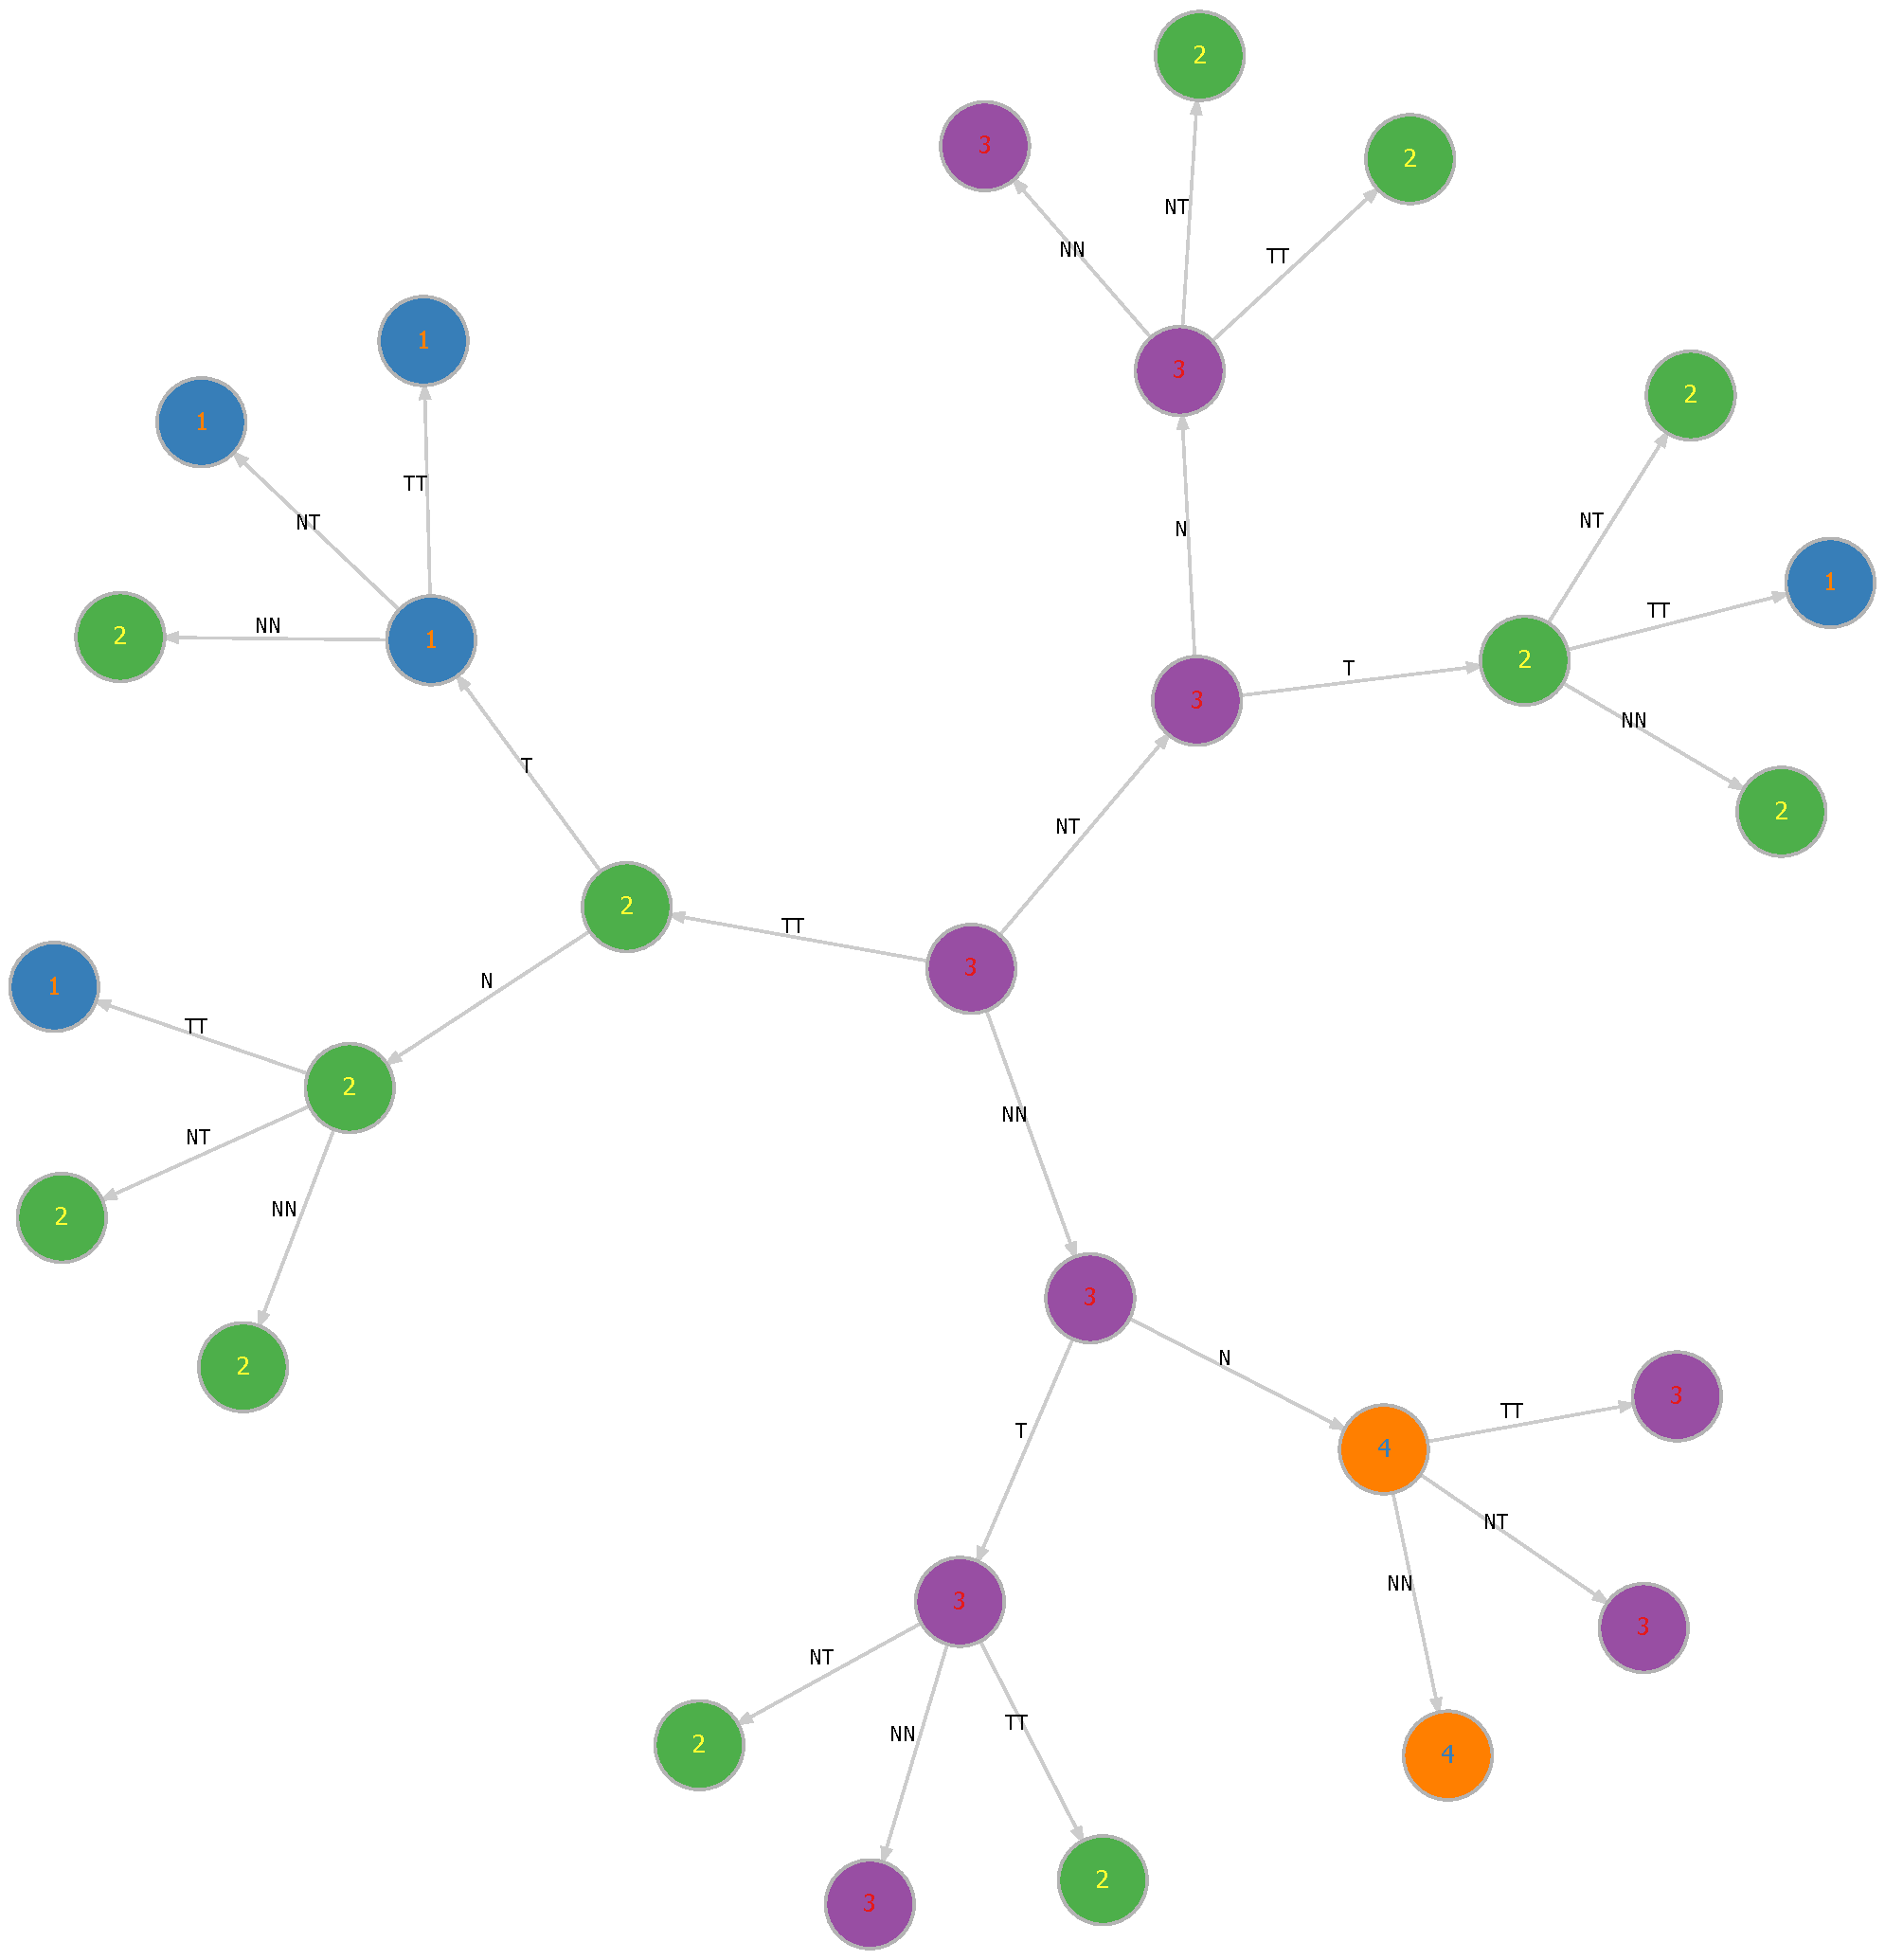
\includegraphics[width=\textwidth]{TITE-DTP-NonUniformDTPNode}
\end{figure}

These DTPs can be interpreted in the same way as before but now just correspond to a different number of patients. Where the recommended dose is set at dose-level 3 for cohort 5 we can consider these pathways equivalent to those presented earlier in Table \ref{tab_tite-dtp:UsingDuringTrialDTPs4-7} for cohort 4. As in both of these scenarios 3 patients would have been treated at dose-level 3. For instance pathways 1-6 and their recommended dose for cohort 6 in Table \ref{tab_tite-dtp:NonUniformDTPs4-7} are equivalent to pathways 1-16 and its recommended dose for cohort 5 in Table \ref{tab_tite-dtp:UsingDuringTrialDTPs4-7}, This is because in both instances 3 patients have been treated at the same dose-level and all have the same outcome. Of course, this does not always hold as a dose decision made on less data may lead to a different dose decision and hence create a different pathway. In the scenarios where two patients experience a DLT the model de-escalates and since there is not a third patient at that dose-level 3 the following pathways will all differ from those presented previously. 

We have established how DTPs can be used during the design and calibration of a trial but also whilst it is running. They have the ability to communicate dose decisions effectively. They also help alleviate some of the potential mystery behind model-based designs where clinicians and non-statisticians involved in trials may not appreciate how dose decisions are being made by a model such as the CRM. Additionally, they can also be used to assess any modifications that need to be implemented due to practical or logistical issues. It is clear DTPs are a valuable tool to incorporate in any dose-finding trial and with the escalation package by Brock \cite{brockModularApproachDose2020} they are very easy to implement, only requiring a few lines of code. 

Yap et al. \cite{yapDoseTransitionPathways2017} briefly discuss the idea of implementing DTPs in TITE-CRMs. However, limited advice or guidance was provided regarding the problems statisticians may face when trying to do this and there were no examples to refer to. In the next section, we explore the possibility of extending DTPs to work in TITE-CRMs using an illustrative example. We also discuss potential limitations and issues faced when attempting this.   

%----------------------------------------------------------------------------------------
%	SECTION 3
%----------------------------------------------------------------------------------------

\section{TITE-DTPs}
\label{tite-dtp:TITE-DTPs}

One reason why DTPs are effective is due to the simplicity of the outcomes being presented. With a CRM these outcomes are either toxicity (T) or no toxicity (N). Similarly, with a design like Wages and Tait or EffTox, outcomes are either toxicity (T), efficacy (E), both toxicity and efficacy (B) or neither (N). Whilst the number of outcomes contributes to the number of potential pathways, other aspects of the trial also go into determining this such as cohort size and the number of cohorts. 

However, when we move to the TITE setting the problem becomes more complex. TITE methodology works by using the idea of a partial tolerance event. At the time of analysis for a dose decision, patients without a toxicity event who have not completed their evaluation period can be considered as having a partial tolerance. These patients can then be weighted according to how much of the evaluation period they have completed and be included in the model. If the patient completes the evaluation period without having a toxicity, they have tolerated treatment and are fully weighted. This means they can be analysed and included in the model as is normally done in a standard CRM design. If a patient experiences a toxicity at any time point they are also fully weighted. 

With TITE-DTPs we still maintain the issues from normal DTPs. The number of cohorts and the cohort sizes determines the number of pathways that are produced, but now the outcome is also more complex. More specifically, just considering DTPs for a standard CRM design, patients would have either a toxicity or no toxicity whereas now in the TITE setting we also have to account for the time each patient has spent in the trial. This problem could also be extended depending on how much precision is used in the measurement of time. 

To explore the problem further we will use an illustrative example. Consider the example trial we presented in Section \ref{tite-dtp:Example-DTPs}, except now we include a TITE component with a 35-day evaluation period. The TITE-CRM can use all the same parameters and specifications we chose for the CRM trial. When setting up a time-to-event trial we also need to specify a weight function. This function determines how patients with partial tolerances will be weighted in the TITE-CRM model. For this example, we will use a standard linear weight function where patients are weighted as a proportion of the time they have completed in the evaluation period. So, a patient who has completed 20 days would have a weight of 0.571 (i.e. $20 \div 35$). The original CRM design used cohorts of three however, due to the complexity of TITE-DTPs we will begin by looking at cohorts of one and two patients. For similar reasoning, we will also only detail pathways for the first cohort. 

%-----------------------------------
%	SUBSECTION 1
%-----------------------------------

\subsection{Cohort of one patient}
\label{tite-dtp:TITE-DTPs-c1}

First we will just look at a cohort of one patient, i.e the first patient recruited into the trial. There are 36 possible outcomes for this patient. The simplest pathway to consider is what happens when this patient has a toxicity, as the timing of the toxicity does not impact how the patient is weighted. In this scenario, the recommended dose for the next patient according to the TITE-CRM model would be dose-level 1. So, if we see toxicity at any time point we de-escalate.   

Now in the scenario where no toxicity is observed, there are 35 different possible outcomes. Either it is day one and the patient has no toxicity, or it is day two, or day three, all the way up to no toxicity at day 35. Here we can fit the TITE-CRM model for each different outcome and see what the model will recommend as the next dose. Where the patient has between 1-19 days of follow-up the model recommends dose-level 4, anything greater than 19 and the model recommends dose-level 5.  

After calculating all possible outcomes we can produce a TITE-DTP for this cohort (Table \ref{tab_tite-dtp:TITEDTP_c1}). As previously specified the first patient starts at dose-level 2, and as there are 36 possible outcomes there are 36 pathways to the next cohort.

We also extend the nomenclature of Brock et al. \cite{brockImplementingEffToxDosefinding2017} to express the different outcomes; here the number in brackets represents the amount of follow-up or observation period the patient has completed. So,  N(14) indicates at 14 days the patient has had a partial tolerance event and the corresponding recommended dose for that pathway is dose-level 4. To summarise a large group of these outcomes we may include inequalities in the notation as well; N($\leq$14) would refer to all the outcomes where the patient had 14 days of follow-up or less. Similarly, N($\geq$14) would indicate 14 days or more. 

\begin{table}[H]
	
	\caption{\label{tab_tite-dtp:TITEDTP_c1}TITE-DTP for a cohort of one.}
	\centering
	\resizebox{0.75\linewidth}{!}{
		\fontsize{4}{3}\selectfont
		\begin{tabular}[t]{cccc}
			\toprule
			\multicolumn{1}{c}{} & \multicolumn{2}{c}{Cohort 1} & \multicolumn{1}{c}{Cohort 2} \\
			\cmidrule(l{3pt}r{3pt}){2-3} \cmidrule(l{3pt}r{3pt}){4-4}
			Pathway & Dose & Outcomes & Dose\\
			\midrule
			\cellcolor{gray!6}{1} & \cellcolor{gray!6}{2} & \cellcolor{gray!6}{T} & \cellcolor{gray!6}{1}\\
			2 & 2 & N(1) & 4\\
			\cellcolor{gray!6}{3} & \cellcolor{gray!6}{2} & \cellcolor{gray!6}{N(2)} & \cellcolor{gray!6}{4}\\
			4 & 2 & N(3) & 4\\
			\cellcolor{gray!6}{5} & \cellcolor{gray!6}{2} & \cellcolor{gray!6}{N(4)} & \cellcolor{gray!6}{4}\\
			6 & 2 & N(5) & 4\\
			\cellcolor{gray!6}{7} & \cellcolor{gray!6}{2} & \cellcolor{gray!6}{N(6)} & \cellcolor{gray!6}{4}\\
			8 & 2 & N(7) & 4\\
			\cellcolor{gray!6}{9} & \cellcolor{gray!6}{2} & \cellcolor{gray!6}{N(8)} & \cellcolor{gray!6}{4}\\
			10 & 2 & N(9) & 4\\
			\cellcolor{gray!6}{11} & \cellcolor{gray!6}{2} & \cellcolor{gray!6}{N(10)} & \cellcolor{gray!6}{4}\\
			12 & 2 & N(11) & 4\\
			\cellcolor{gray!6}{13} & \cellcolor{gray!6}{2} & \cellcolor{gray!6}{N(12)} & \cellcolor{gray!6}{4}\\
			14 & 2 & N(13) & 4\\
			\cellcolor{gray!6}{15} & \cellcolor{gray!6}{2} & \cellcolor{gray!6}{N(14)} & \cellcolor{gray!6}{4}\\
			16 & 2 & N(15) & 4\\
			\cellcolor{gray!6}{17} & \cellcolor{gray!6}{2} & \cellcolor{gray!6}{N(16)} & \cellcolor{gray!6}{4}\\
			18 & 2 & N(17) & 4\\
			\cellcolor{gray!6}{19} & \cellcolor{gray!6}{2} & \cellcolor{gray!6}{N(18)} & \cellcolor{gray!6}{4}\\
			20 & 2 & N(19) & 4\\
			\cellcolor{gray!6}{21} & \cellcolor{gray!6}{2} & \cellcolor{gray!6}{N(20)} & \cellcolor{gray!6}{5}\\
			22 & 2 & N(21) & 5\\
			\cellcolor{gray!6}{23} & \cellcolor{gray!6}{2} & \cellcolor{gray!6}{N(22)} & \cellcolor{gray!6}{5}\\
			24 & 2 & N(23) & 5\\
			\cellcolor{gray!6}{25} & \cellcolor{gray!6}{2} & \cellcolor{gray!6}{N(24)} & \cellcolor{gray!6}{5}\\
			26 & 2 & N(25) & 5\\
			\cellcolor{gray!6}{27} & \cellcolor{gray!6}{2} & \cellcolor{gray!6}{N(26)} & \cellcolor{gray!6}{5}\\
			28 & 2 & N(27) & 5\\
			\cellcolor{gray!6}{29} & \cellcolor{gray!6}{2} & \cellcolor{gray!6}{N(28)} & \cellcolor{gray!6}{5}\\
			30 & 2 & N(29) & 5\\
			\cellcolor{gray!6}{31} & \cellcolor{gray!6}{2} & \cellcolor{gray!6}{N(30)} & \cellcolor{gray!6}{5}\\
			32 & 2 & N(31) & 5\\
			\cellcolor{gray!6}{33} & \cellcolor{gray!6}{2} & \cellcolor{gray!6}{N(32)} & \cellcolor{gray!6}{5}\\
			34 & 2 & N(33) & 5\\
			\cellcolor{gray!6}{35} & \cellcolor{gray!6}{2} & \cellcolor{gray!6}{N(34)} & \cellcolor{gray!6}{5}\\
			36 & 2 & N & 5\\
			\bottomrule
	\end{tabular}}
\end{table}

DTPs presented earlier in this chapter have been able to convey a lot of information. Previously with 64 pathways, we were able to specify all the possible outcomes and dose recommendations up to the 4th cohort of three patients. Whereas in the TITE setting, we have 36 just for one cohort of one patient. One way to improve on this would be to more succinctly summarise the TITE-DTP by aggregating the pathways which lead to the same recommendations. Table \ref{tab_tite-dtp:TITEDTP_c1_Sum} does this for us. 

\begin{table}[H]
	\centering
	\caption{Summary of TITE-DTP for a cohort of one.}
	\label{tab_tite-dtp:TITEDTP_c1_Sum}
	\begin{tabular}{ccccc}
		\hline
		\multicolumn{1}{l}{} &                 & \multicolumn{2}{c}{Cohort 1}   & Cohort 2 \\ 
		\cmidrule(l{3pt}r{3pt}){3-4} \cmidrule(l{3pt}r{3pt}){5-5}
		No. of Pathways & Dose                 & Outcome            & Follow-up & Dose     \\ \hline
		1				&  2                   & T                  &           & 1        \\ \hline
		19				&  \multirow{2}{*}{2}  & \multirow{2}{*}{N} & 1-19      & 4        \\
		16				&	 				   &                    & 20-35     & 5        \\ \hline
	\end{tabular}
\end{table}

Whilst we can still apply the concept of DTPs to TITE-CRMs we can see even with just one patient and one cohort there are a lot of possible outcomes we have to look at. Also, we have used a fairly small observation period of only 5 weeks. If a larger observation period were to be used the number of pathways can get out of hand very quickly. In the next section, we explore how adding in an extra patient affects these TITE-DTPs.  

%-----------------------------------
%	SUBSECTION 2
%-----------------------------------

\subsection{Cohort of two patients}
\label{tite-dtp:TITE-DTPs-c2}
Now we consider a cohort of two patients who start at dose-level 2. As before we will consider this the first cohort of patients and only calculate pathways for the next cohort. Here the number of outcomes is a lot greater. There are three potential scenarios either both patients could have a toxicity, one of the patients could have a toxicity and one could not and finally both patients could have no toxicity. Within the two options where patients could potentially have no toxicity, there are multiple outcomes depending on how much follow-up time is observed. The different scenarios and the associated number of outcomes are: 

\begin{itemize}
	\item TT - 1 outcome 
	\item NT - 35 outcomes 
	\item NN - 630 outcomes
\end{itemize}

So, for a cohort of two patients with a follow-up period of 35 days, there are 666 possible pathways. The simplest of these is if both patients have a toxicity. Here both patients are fully weighted and when put into the model the dose recommendation is dose-level 1. 

If one patient has a toxicity and the other one does not there will be 35 different outcomes. One patient has a toxicity and the other has a partial tolerance event on day one, day two, day three, all the way till day 35 where they have fully tolerated the dose (i.e. N(1)T, N(2)T, N(3)T, ..., N(34)T, NT). These outcomes are just an extension of the pathways in Section \ref{tite-dtp:TITE-DTPs-c1} for one cohort of one patient, except now when we model these we include an extra patient in the model who experienced a toxicity. Table \ref{tab_tite-dtp:TITEDTP_c2NT} presents the pathways for this scenario. Here we can see, regardless of how much follow-up time the patient with no toxicity has, the model will always recommend de-escalating. 

\begin{table}[H]
	
	\caption{\label{tab_tite-dtp:TITEDTP_c2NT}TITE-DTP for a cohort of two for scenario 2NT.}
	\centering
	\resizebox{0.75\linewidth}{!}{
		\fontsize{4}{3}\selectfont
		\begin{tabular}[t]{cccc}
			\toprule
			\multicolumn{1}{c}{} & \multicolumn{2}{c}{Cohort 1} & \multicolumn{1}{c}{Cohort 2} \\
			\cmidrule(l{3pt}r{3pt}){2-3} \cmidrule(l{3pt}r{3pt}){4-4}
			Pathway & Dose & Outcomes & Dose\\
			\midrule
			\cellcolor{gray!6}{1} & \cellcolor{gray!6}{2} & \cellcolor{gray!6}{N(1)T} & \cellcolor{gray!6}{1}\\
			2 & 2 & N(2)T & 1\\
			\cellcolor{gray!6}{3} & \cellcolor{gray!6}{2} & \cellcolor{gray!6}{N(3)T} & \cellcolor{gray!6}{1}\\
			4 & 2 & N(4)T & 1\\
			\cellcolor{gray!6}{5} & \cellcolor{gray!6}{2} & \cellcolor{gray!6}{N(5)T} & \cellcolor{gray!6}{1}\\
			6 & 2 & N(6)T & 1\\
			\cellcolor{gray!6}{7} & \cellcolor{gray!6}{2} & \cellcolor{gray!6}{N(7)T} & \cellcolor{gray!6}{1}\\
			8 & 2 & N(8)T & 1\\
			\cellcolor{gray!6}{9} & \cellcolor{gray!6}{2} & \cellcolor{gray!6}{N(9)T} & \cellcolor{gray!6}{1}\\
			10 & 2 & N(10)T & 1\\
			\cellcolor{gray!6}{11} & \cellcolor{gray!6}{2} & \cellcolor{gray!6}{N(11)T} & \cellcolor{gray!6}{1}\\
			12 & 2 & N(12)T & 1\\
			\cellcolor{gray!6}{13} & \cellcolor{gray!6}{2} & \cellcolor{gray!6}{N(13)T} & \cellcolor{gray!6}{1}\\
			14 & 2 & N(14)T & 1\\
			\cellcolor{gray!6}{15} & \cellcolor{gray!6}{2} & \cellcolor{gray!6}{N(15)T} & \cellcolor{gray!6}{1}\\
			16 & 2 & N(16)T & 1\\
			\cellcolor{gray!6}{17} & \cellcolor{gray!6}{2} & \cellcolor{gray!6}{N(17)T} & \cellcolor{gray!6}{1}\\
			18 & 2 & N(18)T & 1\\
			\cellcolor{gray!6}{19} & \cellcolor{gray!6}{2} & \cellcolor{gray!6}{N(19)T} & \cellcolor{gray!6}{1}\\
			20 & 2 & N(20)T & 1\\
			\cellcolor{gray!6}{21} & \cellcolor{gray!6}{2} & \cellcolor{gray!6}{N(21)T} & \cellcolor{gray!6}{1}\\
			22 & 2 & N(22)T & 1\\
			\cellcolor{gray!6}{23} & \cellcolor{gray!6}{2} & \cellcolor{gray!6}{N(23)T} & \cellcolor{gray!6}{1}\\
			24 & 2 & N(24)T & 1\\
			\cellcolor{gray!6}{25} & \cellcolor{gray!6}{2} & \cellcolor{gray!6}{N(25)T} & \cellcolor{gray!6}{1}\\
			26 & 2 & N(26)T & 1\\
			\cellcolor{gray!6}{27} & \cellcolor{gray!6}{2} & \cellcolor{gray!6}{N(27)T} & \cellcolor{gray!6}{1}\\
			28 & 2 & N(28)T & 1\\
			\cellcolor{gray!6}{29} & \cellcolor{gray!6}{2} & \cellcolor{gray!6}{N(29)T} & \cellcolor{gray!6}{1}\\
			30 & 2 & N(30)T & 1\\
			\cellcolor{gray!6}{31} & \cellcolor{gray!6}{2} & \cellcolor{gray!6}{N(31)T} & \cellcolor{gray!6}{1}\\
			32 & 2 & N(32)T & 1\\
			\cellcolor{gray!6}{33} & \cellcolor{gray!6}{2} & \cellcolor{gray!6}{N(33)T} & \cellcolor{gray!6}{1}\\
			34 & 2 & N(34)T & 1\\
			\cellcolor{gray!6}{35} & \cellcolor{gray!6}{2} & \cellcolor{gray!6}{NT} & \cellcolor{gray!6}{1}\\
			\bottomrule
	\end{tabular}}
\end{table}

The most complicated scenario is when both patients have no toxicity. The number of outcomes for this scenario can be calculated using the combinations with replacement formula where n represents the number of follow-up days and r represents the number of patients: 

\begin{equation}
	\label{eq_tite-dtp:combinations}
	\mathbb{C}(n+r-1,r) = \frac{(n+r-1)!}{r!(n-1)!}
\end{equation}

Here we have to consider every combination of follow-up days both patients could have completed. We only consider unique combinations of days for example, N(21)N(34) would indicate one patient had been observed for 21 days and the other for 34 days, this would be the same as N(34)N(21) and so would only require one pathway. 

For our example with two patients and an observation window of 35 days, we get 630 different combinations, hence the 630 pathways. Trying to show all these pathways in a table as we did before would be infeasible and hard to interpret so instead we just present the aggregate dose recommendations in Table \ref{tab_tite-dtp:TITEDTP_c2NN}. 

\begin{table}[H]
	\centering
	\caption{Summary of pathways for a cohort of two for scenario 2NN.}
	\label{tab_tite-dtp:TITEDTP_c2NN}
	\begin{tabular}{cccc}
		\hline
		\multicolumn{1}{l}{} & \multicolumn{1}{l}{} & \multicolumn{2}{c}{Combined no. of Follow-up Days} \\ \cline{3-4} 
		Recommend Dose & No. of Pathways & Minimum & Maximum \\ \hline
		4              & 102             & 2       & 21      \\
		5              & 528             & 20      & 70      \\ \hline
	\end{tabular}
\end{table}

We can see out of the 630 pathways, 102 recommend dose 4 for the next cohort and 528 recommend dose 5. Dose-level 4 is recommended when the combined follow-up between patients is between 2 and 21 days and dose-level 5 is recommended when the combined number of follow-up days is between 20 and 70. This presents another problem with TITE-DTPs, as there is some overlap in dose recommendations depending on how much combined follow-up patients have. So, if the combined follow-up between the two patients in the cohort is 20 or 21 days they could potentially be allocated to either dose-level 4 or 5 and the way that decision is made is dependent on the split in follow-up between the two patients. This problem is also visualised in Figure \ref{fig_tite-dtp:c2NNprob}. The red lines indicate the combined follow-up time between both patients of 19 and 22 days respectively. Anything greater than 22 days combined follow-up and the model recommends dose-level 5, anything less than 19 and the recommendation is dose-level 4. In between those two time points is a bit of a grey area with the model selecting to escalate higher, to dose-level 5, with less data i.e. combined follow-up time of 20 days. Table \ref{tab_tite-dtp:TITEDTP_c2NNprob} provides a breakdown of these specific combinations. 

\begin{figure}[h!]
	\centering
	\caption[Combined follow-up and dose decisions for a cohort of two.]{Plot illustrating combined-follow up and overlap of dose recommendations for a cohort of two patients for scenario NN.}
	\label{fig_tite-dtp:c2NNprob}
	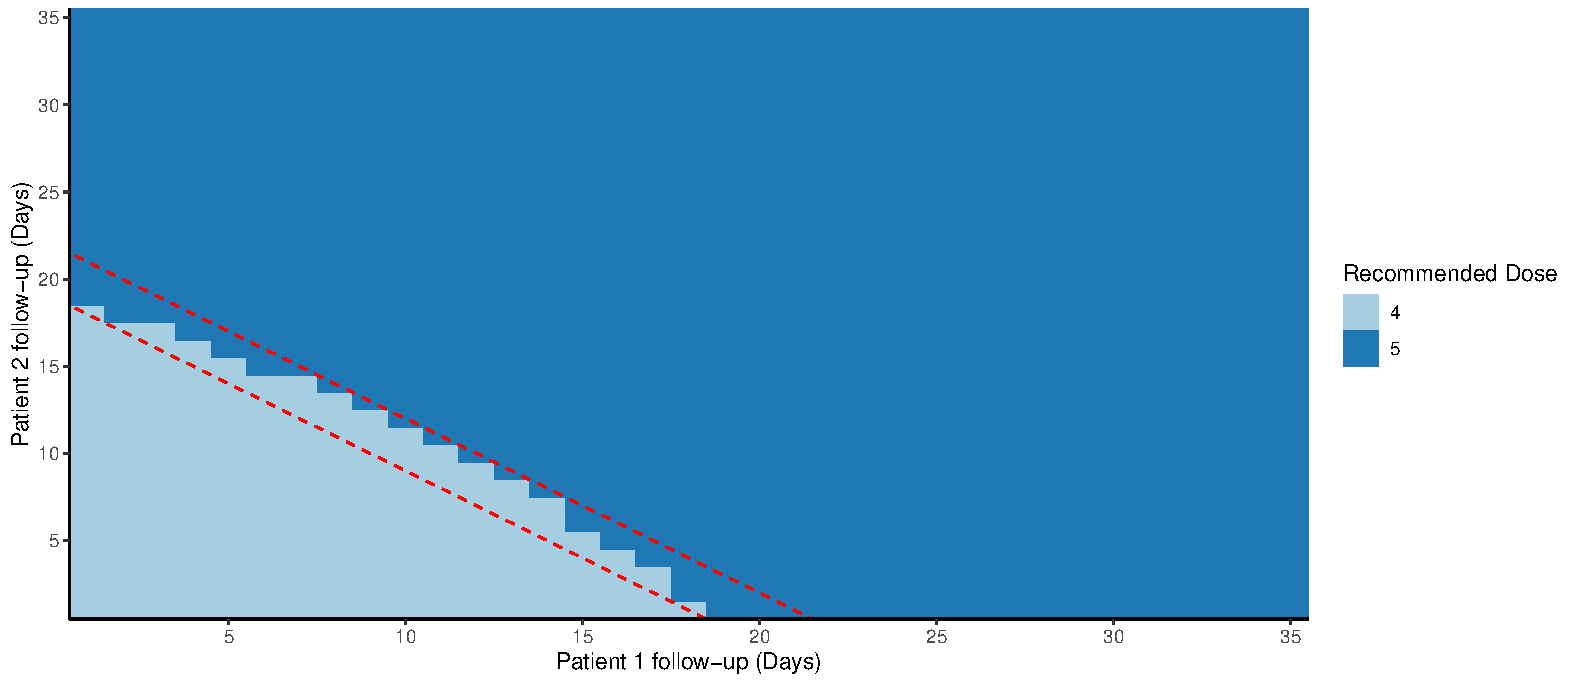
\includegraphics[width=\textwidth]{TITE-DTP-c2NN}
\end{figure}

\begin{table}[H]
	
	\caption{\label{tab_tite-dtp:TITEDTP_c2NNprob}Different dose recommendations with overlapping combined follow-up times.}
	\centering
	\fontsize{11}{13}\selectfont
	\begin{tabular}[t]{cccccc}
		\toprule
		\multicolumn{3}{c}{Follow-up} & \multicolumn{1}{c}{ } & \multicolumn{2}{c}{Posterior Estimates} \\
		\cmidrule(l{3pt}r{3pt}){1-3} \cmidrule(l{3pt}r{3pt}){5-6}
		Patient 1 & Patient 2 & Combined & Dose Recommendation & $\beta$ & Variance\\
		\midrule
		\cellcolor{gray!6}{1} & \cellcolor{gray!6}{20} & \cellcolor{gray!6}{21} & \cellcolor{gray!6}{5} & \cellcolor{gray!6}{0.1606} & \cellcolor{gray!6}{1.2024}\\
		2 & 19 & 21 & 5 & 0.1579 & 1.2063\\
		\cellcolor{gray!6}{3} & \cellcolor{gray!6}{18} & \cellcolor{gray!6}{21} & \cellcolor{gray!6}{5} & \cellcolor{gray!6}{0.1555} & \cellcolor{gray!6}{1.2097}\\
		4 & 17 & 21 & 5 & 0.1534 & 1.2127\\
		\cellcolor{gray!6}{5} & \cellcolor{gray!6}{16} & \cellcolor{gray!6}{21} & \cellcolor{gray!6}{5} & \cellcolor{gray!6}{0.1516} & \cellcolor{gray!6}{1.2153}\\
		6 & 15 & 21 & 5 & 0.1501 & 1.2174\\
		\cellcolor{gray!6}{7} & \cellcolor{gray!6}{14} & \cellcolor{gray!6}{21} & \cellcolor{gray!6}{4} & \cellcolor{gray!6}{0.1489} & \cellcolor{gray!6}{1.2191}\\
		8 & 13 & 21 & 4 & 0.1480 & 1.2204\\
		\cellcolor{gray!6}{9} & \cellcolor{gray!6}{12} & \cellcolor{gray!6}{21} & \cellcolor{gray!6}{4} & \cellcolor{gray!6}{0.1474} & \cellcolor{gray!6}{1.2212}\\
		10 & 11 & 21 & 4 & 0.1471 & 1.2216\\
		\cellcolor{gray!6}{1} & \cellcolor{gray!6}{19} & \cellcolor{gray!6}{20} & \cellcolor{gray!6}{5} & \cellcolor{gray!6}{0.1520} & \cellcolor{gray!6}{1.2110}\\
		2 & 18 & 20 & 5 & 0.1495 & 1.2146\\
		\cellcolor{gray!6}{3} & \cellcolor{gray!6}{17} & \cellcolor{gray!6}{20} & \cellcolor{gray!6}{4} & \cellcolor{gray!6}{0.1473} & \cellcolor{gray!6}{1.2178}\\
		4 & 16 & 20 & 4 & 0.1453 & 1.2205\\
		\cellcolor{gray!6}{5} & \cellcolor{gray!6}{15} & \cellcolor{gray!6}{20} & \cellcolor{gray!6}{4} & \cellcolor{gray!6}{0.1437} & \cellcolor{gray!6}{1.2228}\\
		6 & 14 & 20 & 4 & 0.1424 & 1.2247\\
		\cellcolor{gray!6}{7} & \cellcolor{gray!6}{13} & \cellcolor{gray!6}{20} & \cellcolor{gray!6}{4} & \cellcolor{gray!6}{0.1414} & \cellcolor{gray!6}{1.2261}\\
		8 & 12 & 20 & 4 & 0.1406 & 1.2272\\
		\cellcolor{gray!6}{9} & \cellcolor{gray!6}{11} & \cellcolor{gray!6}{20} & \cellcolor{gray!6}{4} & \cellcolor{gray!6}{0.1402} & \cellcolor{gray!6}{1.2278}\\
		10 & 10 & 20 & 4 & 0.1400 & 1.2280\\
		\bottomrule
	\end{tabular}
\end{table}

In the case where one patient has 14 days or less of follow-up, the model recommends dose-level 4, similarly, if one patient has at least 18 days of follow up the model recommends dose-level 5. Then when one patient has follow-up times of 15, 16 or 17 the model requires the second patient to have enough follow-up to make the combined total of 21 days in order to recommend dose-level 5. So, there exists some threshold whereby the model is happy to escalate further if a single patient has enough follow-up (in this case 18 days) and some critical range where the model will only escalate further if a minimum combined follow-up threshold is met (here this is between 15-17 days for one patient with the threshold being 21 days).

This could perhaps be similar to an incoherent CRM design, which escalates after observing a toxicity, except here we escalate after an inadequate amount of follow-up. It should also be noted that in practice rules may be employed to stop the trial skipping untried doses or skipping multiple doses which is what is being recommended in this case. However, that does not mean that this issue would still not occur even when selecting between two more appropriate dose-levels. 

This issue was examined further by assessing the posterior estimates of our model parameter $\beta$ and it's variance, from the power model used within our TITE-CRM, for each of these different follow-up combinations. Table \ref{tab_tite-dtp:TITEDTP_c2NNprob} shows these values. What can be seen is that there is a specific value of $\beta$ at which point the dose-decision changes from dose-level 4 to 5. The skeleton is updated using the power model and the estimate of $\beta$ to generate posterior probabilities of toxicity for each dose. The dose-level then closest to our target of 25\% is then selected as the recommended dose. So, there must exist some value of $\beta$ at which dose-level 5 now becomes the dose closest to our target. From Table \ref{tab_tite-dtp:TITEDTP_c2NNprob} we can see that a $\beta$ value less than or equal to 0.1489 leads to a dose-recommendation of 4 and a value of 0.1495 or higher leads to a dose recommendation of 5. More specifically, we evaluated values between 0 and 1 up to four decimal places to see exactly where this boundary occurs and found that a $\beta$ value of 0.1492 or lower leads to dose-level 4 and 0.1493 and higher leads to dose-level 5. 

In Figure \ref{fig_tite-dtp:c2NNEstAllCombs} for each possible combination of follow-up from 2 to 70 days we plotted the estimated value of $\beta$ as a single point. For specific combinations of combined follow-up time there is only one way to get to that total value and so there is only one point on the plot. For other combinations there are multiple ways to achieve that so we can see multiple points in these instances. For example, 35 days can be achieved with one patient having 20 and the other 15, or 13 and 22, or 31 and 4 so for these combinations we can see multiple points on the plot. The red line indicates that critical value of 0.1492 and we can see that any combination of follow-up on or before that line recommends dose-level 4 and any above it recommends dose-level 5. 

Figure \ref{fig_tite-dtp:c2NNEst2021} focuses specifically on a combined follow-up time of 20 and 21 days and shows how these two combinations of days are the only ones which cross this critical threshold. Each point on the plot is labelled with the individual days of follow-up for both patients. This is essentially a zoomed in snapshot of Figure \ref{fig_tite-dtp:c2NNEstAllCombs} highlighting the combined follow-up times of 20 and 21 days. 

\begin{figure}[h!]
	\centering
	\caption[Changes in $\beta$ based on combined follow-up for two patients.]{Plot illustrating how the posterior estimate of $\beta$ and dose recommendation change based on combined follow-up for two patients.}
	\label{fig_tite-dtp:c2NNEstAllCombs}
	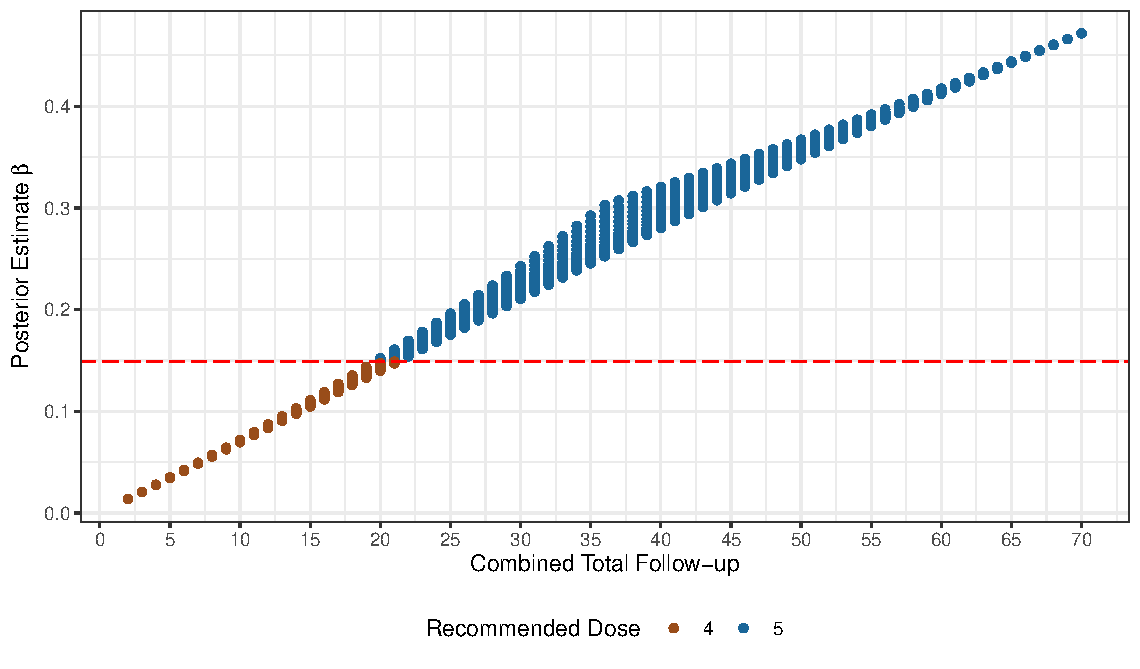
\includegraphics[width=\textwidth]{TITE-DTP-c2NN-EstAllCombs}
\end{figure}

\begin{figure}[h!]
	\centering
	\caption[Changes in $\beta$ based on combined follow-up of 20 and 21 days for two patients.]{Plot illustrating how the posterior estimate of $\beta$ and dose recommendation change based on combined follow-up of 20 and 21 days for two patients.}
	\label{fig_tite-dtp:c2NNEst2021}
	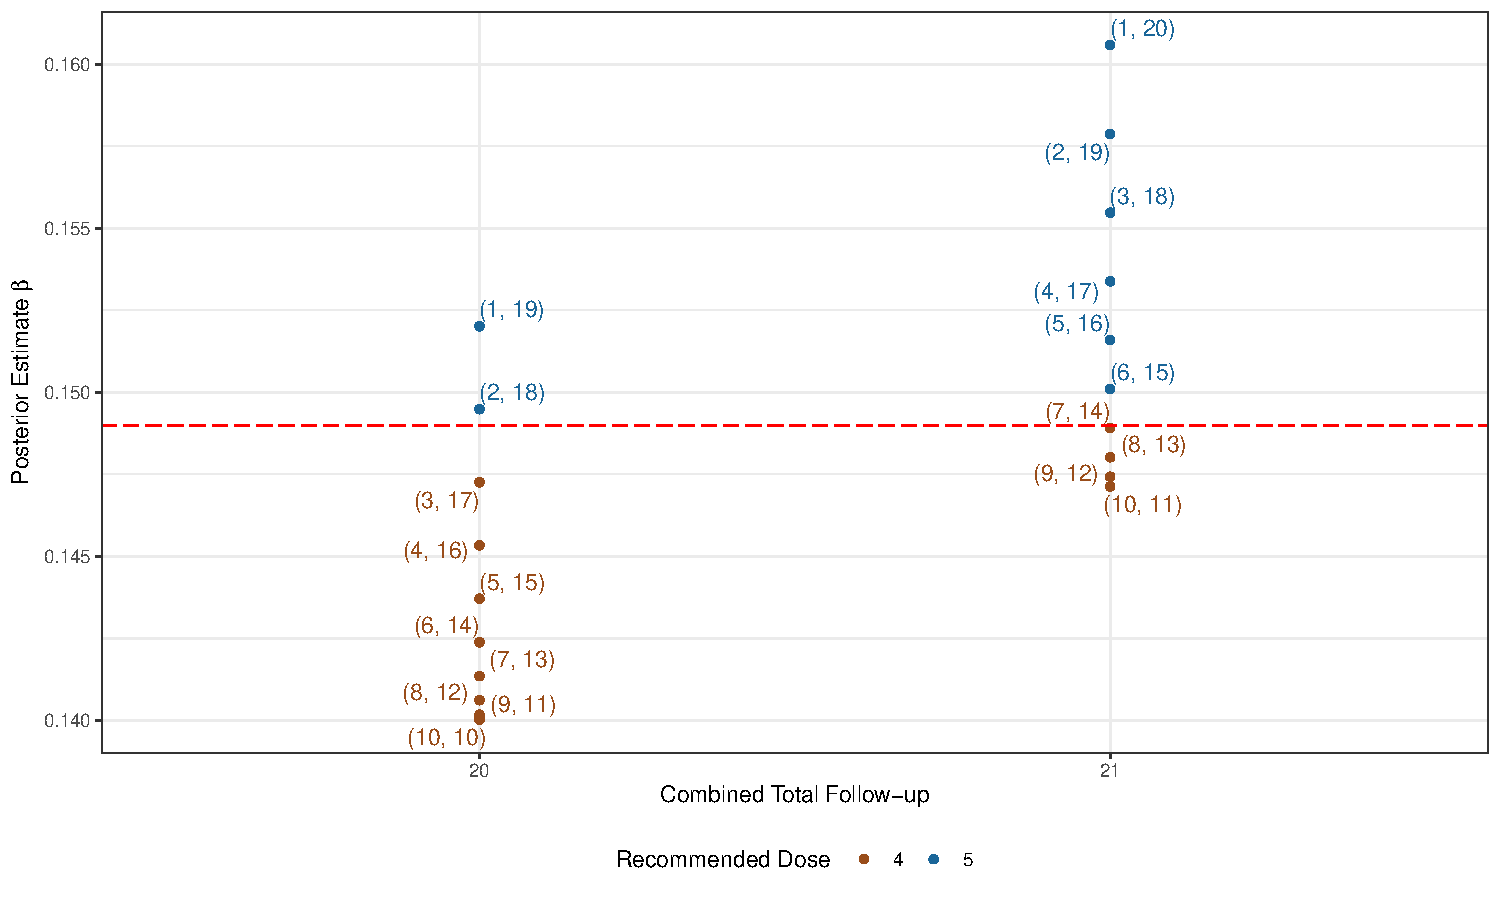
\includegraphics[width=\textwidth]{TITE-DTP-c2NN-Est2021}
\end{figure}

Intuitively, since we are using a linear weight function, we would expect each day of follow-up to be weighted the same across each patient. That is to say if we observe 20 days of follow-up with no toxicity the model should make the same recommendation regardless of if that is 20 patients with only one day of follow-up each or only one patient with 20 days of follow-up. Clearly, that is not the case here. To add to this as well, when we look back at dose transition pathways for a cohort of one (Table \ref{tab_tite-dtp:TITEDTP_c1}) for N(20) and N(21) the model recommends dose-level 5. So, when two patients have a combined (i.e total) follow-up time of 20 or 21 days the dose recommendation could potentially be lower than if just one patient had the same amount of follow-up.   

In order to explore why this discrepancy exists we look into how the TITE-CRM works. For reference the TITE-CRM was originally introduced by Cheung and Chappel \cite{cheungSequentialDesignsPhase2000}. A further detailed description of the TITE-CRM is also provided by Cheung \cite{cheungDoseFindingContinual2011}. We also detail the TITE-CRM design in the presence of partial orders in Chapter \ref{Adept} (Section \ref{adept:PO-TITE-CRM-Design}). The TITE-CRM makes use of a weighted likelihood for the model parameter $\beta$, this is given by the equation below: 

\begin{equation}
	\label{eq_tite-dtp:titelikelihood}
	{L}_n(\beta|w)=\prod_{i=1}^{n}\{w_i F(x_i,\beta)\}^{Y_i} \{1-w_i F(x_i,\beta)\}^{1-Y_i}
\end{equation}

where $F(x_i, \beta)$ is our dose toxicity model, $Y_i$ is a toxicity indicator for each patient and $w_i$ is the weight associated for the observation of each patient. When there are no toxicities i.e. $Y_i = 0$ the first part of the likelihood formula ($w_iF(x_i,\beta)^{Y_i}$) is reduced to 1 and we are left with $1- w_iF(x_i,\beta)^{1-Y_i}$. At each dose-level $F(x_i, \beta)$ will remain fixed and is only affected by the weight $w_i$. This value is different for each patient depending on how long they have been observed in the trial. Then the likelihood is calculated by multiplying these terms for each patient together. This leads us to the root of the issue. As each $w_i$ is independent for each patient and each of these terms is then multiplied together there is no linear relationship between the combined follow-up times for patients at the same dose-level. So, we will get different likelihood estimates which leads to different estimates of the $\beta$ parameter which ultimately leads to different dose decisions as illustrated in our example. 

This was shown in Figure \ref{fig_tite-dtp:c2NNEstAllCombs}, where all combinations of follow-up times yielded different values of $\beta$. For example, a combined total follow-up of 20 days where one patient has 2 days and the other has 18 equates to weights of $\frac{2}{35}$ and $\frac{18}{35}$ for each patient respectively (this is based on our linear weight function and observation window of 35 days). For the same combined total follow-up of 20 days but split where one patient has 3 days and the other has 17 leads to weights of $\frac{3}{35}$ and $\frac{17}{35}$. For these two different combinations when they are plugged into the likelihood formula we would get different results. The plot also shows this occurs at every combination. However, in most instances the different values of $\beta$ for the same overall combined follow-up time would either be all above or below the critical value we discovered so as such would not change the dose decision. 

When using a linear weight function we cannot say that each day in each patient at the same dose-level is worth the same amount. Essentially, the sum of follow-up time between patients at the same dose-level cannot be thought of as the same. 10 days of follow-up in one patient and 10 days in another is not the same as 20 days in one patient or 19 days in one patient and one in another. This is mainly due to how the likelihood is calculated. We can still say that weighting is linear in individual patients, due to the linear weight function we use, this just does not apply across patients. 
 
So far we have split up the presentation of the pathways dependent on the scenario as there are too many to tabulate and present at once. Table \ref{tab_tite-dtp:TITEDTP_c2_Sum} attempts to summarise all the different pathways for a cohort of two patients. However, due to the issue with the NN scenario, it is difficult to adequately summarise the combined follow-up required for the different dose decisions. Here we have opted to show the exact minimum and maximum combined follow-up that leads to different dose-recommendations. We then add in extra rows to provide a specific breakdown of how many days individual patients need.  

From these values you can still determine the minimum and maximum that guarantee a specific dose as well. For a combined follow-up of 20 days where one patient has 17 days or less of follow-up the recommendation is dose-level 4 and for the same combination but with one patient with 18 days or more follow-up the recommendation is dose-level 5. This may be confusing at first as if you assume a combined follow-up of 20 days with one patient only having two days you would say that is less than 17 so the dose-recommendation is 4. However, if one patient has two days and the combination is 20 that implies the other patient has 18 days of follow-up so we should use the recommendation from the N($\geq$18) row which is dose-level 5.

This table could be simplified just by including the overlap in the follow-up column but this would lose out on the granular detail. So, for the outcome NN we could say a follow-up of 2-21 leads to dose-level 4 and a follow-up of 20-70 leads to dose-level 5. An asterisk or some text could accompany the table to perhaps explain the overlap or add more details. 

\begin{table}[H]
	\centering
	\caption{Summary of TITE-DTP for a cohort of two.}
	\label{tab_tite-dtp:TITEDTP_c2_Sum}
	\begin{tabular}{ccccc}
		\hline
		\multicolumn{1}{l}{} &                 \multicolumn{3}{c}{Cohort 1}    & Cohort 2 \\ 
		\cmidrule(l{3pt}r{3pt}){2-4} \cmidrule(l{3pt}r{3pt}){5-5}
		No. of Pathways   & Dose  				& Outcome             & Follow-up 		& Dose     \\ \hline
		1                 & 2               	& TT                  &          		& 1        \\ \hline
		35                & 2            		& NT                  & 1-35      		& 1        \\ \hline
		90   			  & \multirow{6}{*}{2}  & \multirow{6}{*}{NN} & 2-19      		& 4        \\
		8				  &                		&                     & 20 N($\leq$17)  & 4        \\
		4				  &                		&                     & 21 N($\leq$14)  & 4        \\
		2				  &                		&                     & 20 N($\geq$18)  & 5        \\
		6				  &                		&                     & 21 N($\geq$15)  & 5        \\
		520				  &              		&                     & 22-70     		& 5        \\ \hline
	\end{tabular}
\end{table}

As with classic DTPs we can also visually show these pathways. Figure \ref{fig_tite-dtp:TITEDTP-cohort2-node} shows a summary of the pathways as a node plot. Rather than present each possible pathway as we do with normal DTPs here we just present the same summary that is shown in Table \ref{tab_tite-dtp:TITEDTP_c2_Sum}. Inside each node is the dose-level. The arrows show each possible outcome and it's associated dose-decision. Each arrow is labelled with the specific outcome and the combined amount of follow-up time  which leads to the specific recommendation. 

\begin{figure}[h!]
	\centering
	\caption{TITE-DTP Node plot for a cohort of two patients.}
	\label{fig_tite-dtp:TITEDTP-cohort2-node}
	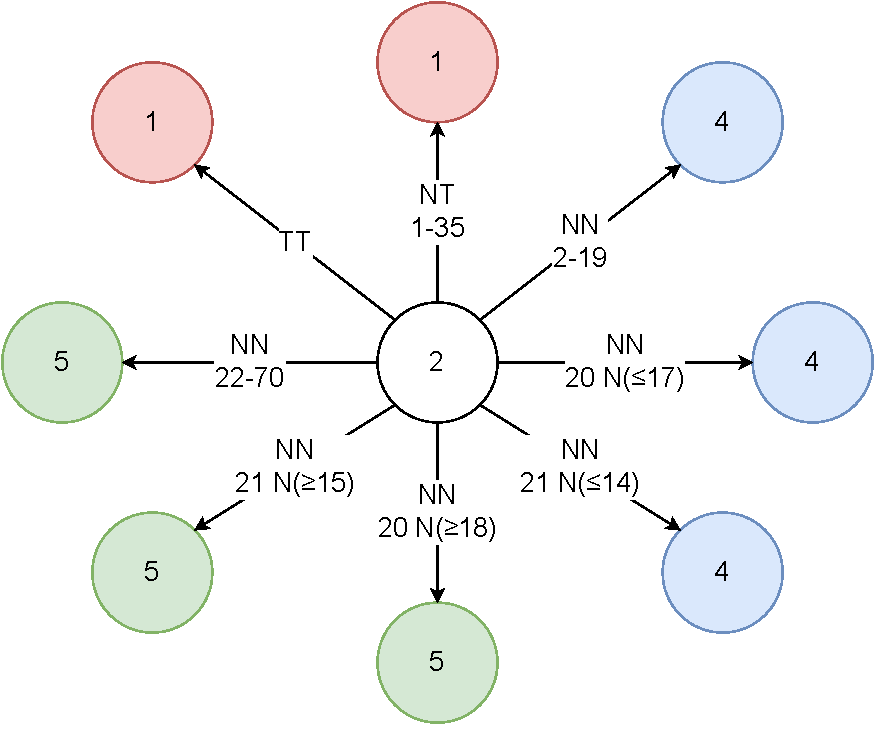
\includegraphics[width=0.9\textwidth]{TITE-DTP-cohort2Node}
\end{figure}


An alternative presentation of the pathways is provided in Figure \ref{fig_tite-dtp:TITEDTP-cohort2-flow}. This plot shows a summary of the pathways in a similar manner to the flow plots of DTPs. It shows how the dose decision changes with the combined amount of follow-up time. Each box is labelled with the specific cohort it is referring to. The number in brackets corresponds to the dose-level and the combined follow-up times required to reach that decision are also listed below the dose-level. Additionally, each box is coloured based on the dose-level that is being recommended for the subsequent cohort. In the case where the boxes are too small we have just contained some relevant details about the specific outcome that leads to that recommendation. 

For this plot it is important to note that follow-up time is only relevant to outcomes of no toxicity (N). So, for TT the outcome is not dependent on follow-up time. However, for NT the outcomes could change based on the amount of follow-up time the patient who experienced no toxicity (N) has. This is why TT, NT and NN have different sized boxes as the total combined follow-up for each is different. Neither of these plots capture how many pathways these outcomes represent but this information could easily be added as required. This should be done with caution as we said before this could be slightly misleading as the number of pathways does not indicate that one outcome is more likely than another. 

Just by adding an extra patient to a cohort of one the number of pathways we have has increased almost 20-fold. We have also discovered when looking at specific combinations of partial tolerance events there are some inconsistencies with the way the TITE-CRM is recommending dose-levels. Finally, for completeness, we attempt producing TITE-DTPs for a cohort of 3 patients.   


\begin{figure}[H]
	\centering
	\caption{TITE-DTP Flow plot for a cohort of two patients.}
	\label{fig_tite-dtp:TITEDTP-cohort2-flow}
	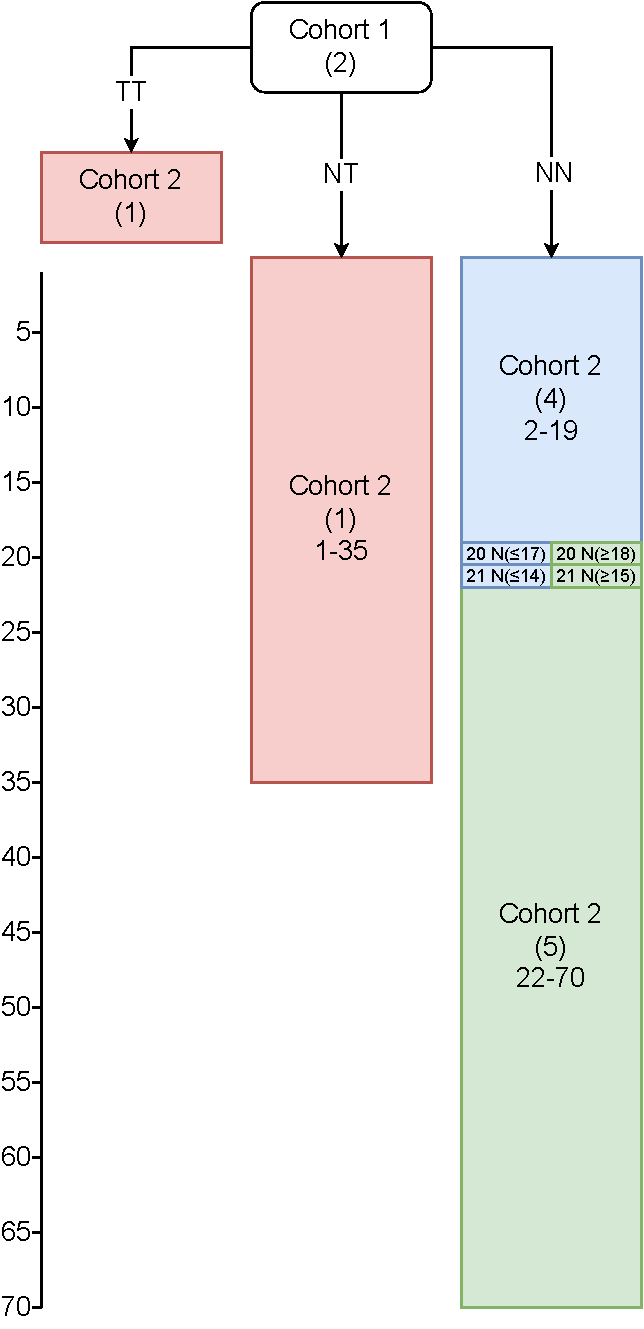
\includegraphics[width=0.8\textwidth, height=\textheight]{TITE-DTP-cohort2Flow}
\end{figure}



%-----------------------------------
%	SUBSECTION 3
%-----------------------------------

\subsection{Cohort of three patients}
Consider instead we have a cohort of 3 patients starting at dose-level 2. Here we will explore all the possible pathways for the first cohort. With 3 patients there are four possible scenarios, the number of possible outcomes relating to each scenario is listed below: 

\begin{itemize}
	\item TTT - 1 outcome 
	\item NTT - 35 outcomes 
	\item NNT - 630 outcomes 
	\item NNN - 7770 outcomes 
\end{itemize}

In total for just the first cohort of three patients, there are 8436 pathways. The first three scenarios listed here are just extensions of what has been previously presented. When all 3 patients have a toxicity, these can just be entered into the model as fully weighted patients and the model recommends de-escalating to dose-level 1. 

The NTT scenario is the same as the cohorts of two NT scenario except now there is an extra patient in the cohort who also has a toxicity. Table \ref{tab_tite-dtp:TITEDTP_c3NTT} shows the pathways for this scenario. Regardless of the number of follow-up days the patient with no toxicity has the model will always recommend dose-level 1 if the other two patients in the cohort have toxicities. 

\begin{table}[H]
	
	\caption{\label{tab_tite-dtp:TITEDTP_c3NTT}TITE-DTP for a cohort of three for scenario 2NTT.}
	\centering
	\resizebox{0.75\linewidth}{!}{
		\fontsize{4}{3}\selectfont
		\begin{tabular}[t]{cccc}
			\toprule
			\multicolumn{1}{c}{} & \multicolumn{2}{c}{Cohort 1} & \multicolumn{1}{c}{Cohort 2} \\
			\cmidrule(l{3pt}r{3pt}){2-3} \cmidrule(l{3pt}r{3pt}){4-4}
			Pathway & Dose & Outcomes & Dose\\
			\midrule
			\cellcolor{gray!6}{1} & \cellcolor{gray!6}{2} & \cellcolor{gray!6}{N(1)TT} & \cellcolor{gray!6}{1}\\
			2 & 2 & N(2)TT & 1\\
			\cellcolor{gray!6}{3} & \cellcolor{gray!6}{2} & \cellcolor{gray!6}{N(3)TT} & \cellcolor{gray!6}{1}\\
			4 & 2 & N(4)TT & 1\\
			\cellcolor{gray!6}{5} & \cellcolor{gray!6}{2} & \cellcolor{gray!6}{N(5)TT} & \cellcolor{gray!6}{1}\\
			6 & 2 & N(6)TT & 1\\
			\cellcolor{gray!6}{7} & \cellcolor{gray!6}{2} & \cellcolor{gray!6}{N(7)TT} & \cellcolor{gray!6}{1}\\
			8 & 2 & N(8)TT & 1\\
			\cellcolor{gray!6}{9} & \cellcolor{gray!6}{2} & \cellcolor{gray!6}{N(9)TT} & \cellcolor{gray!6}{1}\\
			10 & 2 & N(10)TT & 1\\
			\cellcolor{gray!6}{11} & \cellcolor{gray!6}{2} & \cellcolor{gray!6}{N(11)TT} & \cellcolor{gray!6}{1}\\
			12 & 2 & N(12)TT & 1\\
			\cellcolor{gray!6}{13} & \cellcolor{gray!6}{2} & \cellcolor{gray!6}{N(13)TT} & \cellcolor{gray!6}{1}\\
			14 & 2 & N(14)TT & 1\\
			\cellcolor{gray!6}{15} & \cellcolor{gray!6}{2} & \cellcolor{gray!6}{N(15)TT} & \cellcolor{gray!6}{1}\\
			16 & 2 & N(16)TT & 1\\
			\cellcolor{gray!6}{17} & \cellcolor{gray!6}{2} & \cellcolor{gray!6}{N(17)TT} & \cellcolor{gray!6}{1}\\
			18 & 2 & N(18)TT & 1\\
			\cellcolor{gray!6}{19} & \cellcolor{gray!6}{2} & \cellcolor{gray!6}{N(19)TT} & \cellcolor{gray!6}{1}\\
			20 & 2 & N(20)TT & 1\\
			\cellcolor{gray!6}{21} & \cellcolor{gray!6}{2} & \cellcolor{gray!6}{N(21)TT} & \cellcolor{gray!6}{1}\\
			22 & 2 & N(22)TT & 1\\
			\cellcolor{gray!6}{23} & \cellcolor{gray!6}{2} & \cellcolor{gray!6}{N(23)TT} & \cellcolor{gray!6}{1}\\
			24 & 2 & N(24)TT & 1\\
			\cellcolor{gray!6}{25} & \cellcolor{gray!6}{2} & \cellcolor{gray!6}{N(25)TT} & \cellcolor{gray!6}{1}\\
			26 & 2 & N(26)TT & 1\\
			\cellcolor{gray!6}{27} & \cellcolor{gray!6}{2} & \cellcolor{gray!6}{N(27)TT} & \cellcolor{gray!6}{1}\\
			28 & 2 & N(28)TT & 1\\
			\cellcolor{gray!6}{29} & \cellcolor{gray!6}{2} & \cellcolor{gray!6}{N(29)TT} & \cellcolor{gray!6}{1}\\
			30 & 2 & N(30)TT & 1\\
			\cellcolor{gray!6}{31} & \cellcolor{gray!6}{2} & \cellcolor{gray!6}{N(31)TT} & \cellcolor{gray!6}{1}\\
			32 & 2 & N(32)TT & 1\\
			\cellcolor{gray!6}{33} & \cellcolor{gray!6}{2} & \cellcolor{gray!6}{N(33)TT} & \cellcolor{gray!6}{1}\\
			34 & 2 & N(34)TT & 1\\
			\cellcolor{gray!6}{35} & \cellcolor{gray!6}{2} & \cellcolor{gray!6}{NTT} & \cellcolor{gray!6}{1}\\
			\bottomrule
	\end{tabular}}
\end{table}

Similarly, the NNT scenario is an extension of the NN scenario for a cohort of two patients. We add an extra patient who experiences a toxicity and fit the same models and observe the outcomes. Table \ref{tab_tite-dtp:TITEDTP_c3NNT} shows a summary of the 630 possible pathways. We can see that the majority of the time the model recommends de-escalating. However, there are six pathways where the model recommends staying at the same dose, dose-level 2. This is when the combined follow-up time from the two patients who do not have a toxicity is between 67 and 70 days. We also no longer have that inconsistency issue that we saw before where different dose decisions were being made on the same amount of follow-up time dependent on the split of days between patients. Here the TITE DTP is more clear and a combined follow-up time of 66 days or less leads to de-escalation otherwise the next dose should be recruited at the same dose-level.

\begin{table}[H]
	\centering
	\caption{Summary of pathways for a cohort of three for scenario 2NNT. }
	\label{tab_tite-dtp:TITEDTP_c3NNT}
	\begin{tabular}{cccc}
		\hline
		\multicolumn{1}{l}{} & \multicolumn{1}{l}{} & \multicolumn{2}{c}{Combined no. of Follow-up Days} \\ \cline{3-4} 
		Recommend Dose & No. of Pathways & Minimum & Maximum \\ \hline
		1              & 624             & 2       & 66      \\
		2              & 6               & 67      & 70      \\ \hline
	\end{tabular}
\end{table}

When an additional patient is added to the cohort, the most complicated scenario is when all patients in the cohort experience no toxicity. With 3 patients and 35 days follow-up, 7770 different possible combinations of follow-up days can be observed. The results from fitting all these models are presented in Table \ref{tab_tite-dtp:TITEDTP_c3NNN}. In this scenario, if the combined number of follow-up between the three patients is between 3 and 23 days the model will recommend dose-level 4 and if it is above 22 dose-level 5 will be recommended. Again we see the same problem as before with a cohort of two patients for the NN scenario. There appears to be some overlap in dose decisions for certain combinations of follow-up days between the three patients. Anything between 20 and 21 days may result in either a recommendation of dose-level 4 or 5 depending on the split of follow-up time between the three patients. Figure \ref{fig_tite-dtp:c2NNNprob} also provides a 3D illustration of these pathways with each dot representing a different decision, and the colour corresponding to the dose recommended. A dark blue dot indicates dose-level 4 and light blue is dose-level 5.  

\begin{table}[H]
	\centering
	\caption{Summary of pathways for a cohort of three for scenario 2NNN.}
	\label{tab_tite-dtp:TITEDTP_c3NNN}
	\begin{tabular}{cccc}
		\hline
		\multicolumn{1}{l}{} & \multicolumn{1}{l}{} & \multicolumn{2}{c}{Combined no. of Follow-up Days} \\ \cline{3-4} 
		Recommend Dose & No. of Pathways & Minimum & Maximum \\ \hline
		4              & 265             & 3       & 21      \\
		5              & 7505            & 20      & 105      \\ \hline
	\end{tabular}
\end{table}

\begin{figure}[H]
	\centering
	\caption{Dose recommendations for a cohort of three patients for scenario 2NNN.}
	\label{fig_tite-dtp:c2NNNprob}
	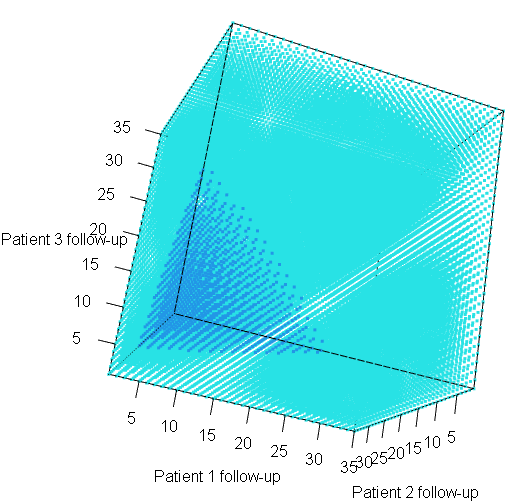
\includegraphics[width=0.8\textwidth]{TITE-DTP-c2NNN}
\end{figure}

In this example, there are 70 different pathways where the combined follow-up between the three patients is 20-21 days. By examining these pathways specifically we can define the different thresholds that are needed to make different decisions. Out of the 70 pathways dose-level 5 is recommended in only 9 of those instances (Table \ref{tab_tite-dtp:TITEDTP_c3NNNprob}). Of those only one is for a combined total follow-up of 20 days and the other 8 have a combined total follow-up of 21 days. So, if one of the three patients has a minimum of 18 days of follow-up then the model will recommend dose-level 5. This is why the minimum combined days of follow-up is 20 to recommend dose-level 5 in Table \ref{tab_tite-dtp:TITEDTP_c3NNN} as one patient will have 18 days and the other two will have one day each. In the case where the combined follow-up is 21 days, the model will only recommend dose-level 5 if one of the three patients has a minimum of 15 days and other has a minimum of 4. 

\begin{table}[H]
	\caption{\label{tab_tite-dtp:TITEDTP_c3NNNprob}Follow-up combinations totalling 20 or 21 days leading to dose-level 5.}
	\centering
	\resizebox{\linewidth}{!}{
		\fontsize{11}{13}\selectfont
		\begin{tabular}[t]{ccccccc}
			\toprule
			\multicolumn{4}{c}{Follow-up} & \multicolumn{1}{c}{ } & \multicolumn{2}{c}{Posterior Estimates} \\
			\cmidrule(l{3pt}r{3pt}){1-4} \cmidrule(l{3pt}r{3pt}){6-7}
			Patient 1 & Patient 2 & Patient 3 & Combined & Dose Recommendation & $\beta$ & Variance\\
			\midrule
			\cellcolor{gray!6}{1} & \cellcolor{gray!6}{1} & \cellcolor{gray!6}{19} & \cellcolor{gray!6}{21} & \cellcolor{gray!6}{5} & \cellcolor{gray!6}{0.1578} & \cellcolor{gray!6}{1.2064}\\
			1 & 2 & 18 & 21 & 5 & 0.1553 & 1.2100\\
			\cellcolor{gray!6}{1} & \cellcolor{gray!6}{3} & \cellcolor{gray!6}{17} & \cellcolor{gray!6}{21} & \cellcolor{gray!6}{5} & \cellcolor{gray!6}{0.1531} & \cellcolor{gray!6}{1.2131}\\
			1 & 4 & 16 & 21 & 5 & 0.1512 & 1.2158\\
			\cellcolor{gray!6}{1} & \cellcolor{gray!6}{5} & \cellcolor{gray!6}{15} & \cellcolor{gray!6}{21} & \cellcolor{gray!6}{5} & \cellcolor{gray!6}{0.1496} & \cellcolor{gray!6}{1.2181}\\
			2 & 2 & 17 & 21 & 5 & 0.1530 & 1.2133\\
			\cellcolor{gray!6}{2} & \cellcolor{gray!6}{3} & \cellcolor{gray!6}{16} & \cellcolor{gray!6}{21} & \cellcolor{gray!6}{5} & \cellcolor{gray!6}{0.1510} & \cellcolor{gray!6}{1.2161}\\
			2 & 4 & 15 & 21 & 5 & 0.1493 & 1.2185\\
			\cellcolor{gray!6}{1} & \cellcolor{gray!6}{1} & \cellcolor{gray!6}{18} & \cellcolor{gray!6}{20} & \cellcolor{gray!6}{5} & \cellcolor{gray!6}{0.1494} & \cellcolor{gray!6}{1.2147}\\
			\bottomrule
	\end{tabular}}
\end{table}

We have not shown all 70 pathways but we observe the $\beta$ estimate in each of these cases leading to a dose recommendation of 5 is above 0.1493. This is the same threshold we saw in the scenario of 2 patients with NN outcomes. Similarly, all of the combinations with $\beta$ estimate of 0.1492 or less resulted in a dose-recommendation of  dose-level 4. As before we can also visualise this issue with Figures \ref{fig_tite-dtp:c2NNNEstAllCombs} and \ref{fig_tite-dtp:c2NNNEst2021}. These plots show the $\beta$ estimates for each possible total follow-up combination and more specifically the combinations for a total of 20 and 21 days. Figure \ref{fig_tite-dtp:c2NNNEst2021} labels each point to show the individual follow-up of each of the patients. Here we see the same pattern before as with the 2NN scenario. A minimum number of days is needed in a specific patient in order to obtain an estimate of $\beta$ which is high enough to warrant escalation to the highest dose. We can see when the follow-up time is split more evenly between the patients the estimates of $\beta$ are lower. This also supports our findings earlier where we surmised that weightings between patients at the same dose-level are not entirely equivalent due to how the likelihood is calculated. 

\begin{figure}[h!]
	\centering
	\caption[Changes in $\beta$ based on combined follow-up for three patients.]{Plot illustrating how the posterior estimate of $\beta$ and dose recommendation change based on combined follow-up for three patients.}
	\label{fig_tite-dtp:c2NNNEstAllCombs}
	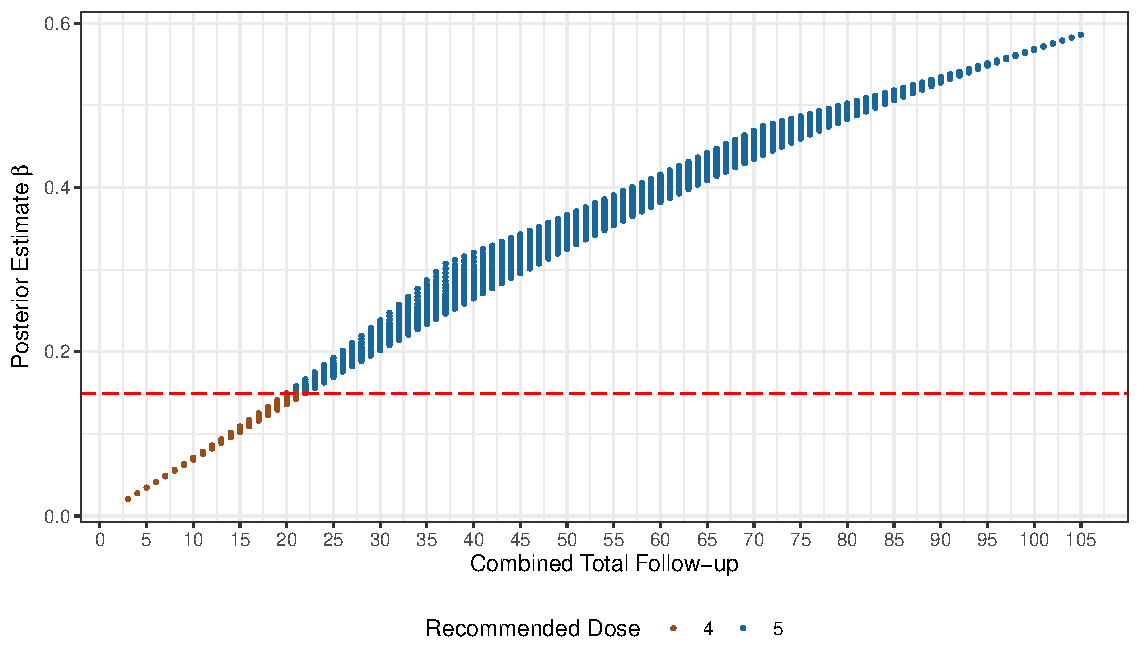
\includegraphics[width=\textwidth]{TITE-DTP-c2NNN-EstAllCombs}
\end{figure}

\begin{figure}[h!]
	\centering
	\caption[Changes in $\beta$ based on combined follow-up of 20 and 21 days for three patients.]{Plot illustrating how the posterior estimate of $\beta$ and dose recommendation change based on combined follow-up of 20 and 21 days for three patients.}
	\label{fig_tite-dtp:c2NNNEst2021}
	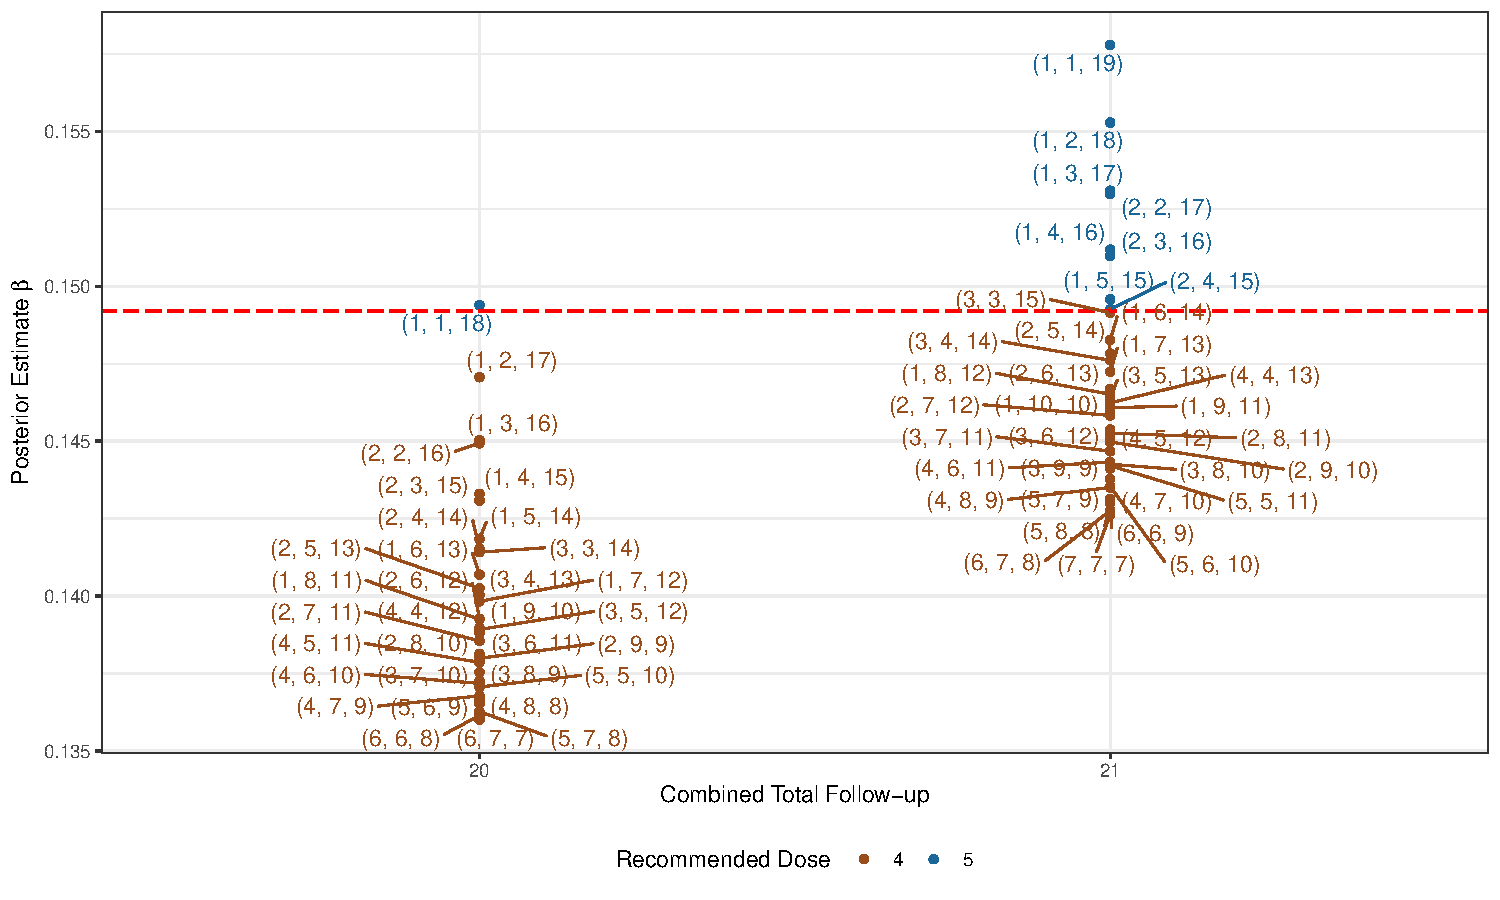
\includegraphics[width=\textwidth]{TITE-DTP-c2NNN-Est2021}
\end{figure}

It is important to note that the threshold of the $\beta$ estimate which causes the change in dose-recommendation should remain constant throughout the trial. This threshold can be thought of as the the values of $\beta$ required to make a dose-recommendation picking between doses 4 and 5. This is what we have observed in our two examples of 2NN and 2NNN outcomes respectively. This is due to the way in which we determine the recommended dose for the next patient. The next dose is recommended based on minimising the following equation: 

\begin{equation}
	|F(d_k, \beta) - \theta| \; k = i, \cdots, 5
\end{equation}

Here $d_k$ represents each dose-level 1 to 5 and $\theta$ is our TD25. The dose with the probability of toxicity closest to our target of 25\% will be selected as our next recommended dose. This probability is determined by our estimate of $\beta$. What we see in our example is that when $\beta$ is less than 0.1492 dose-level 4 is the closest in probability to our target level and when it is 0.1493 or higher it is dose-level 5. We did not observe any values of $\beta$ between 0.1492 and 0.1493 but there must exist some asymptotic value at which the decision changes. This boundary cannot be explicitly defined as its based on the absolute minimum difference which could theoretically be infinitesimally small.    

You would also expect there to be similar boundaries/thresholds when choosing between any two other adjoining dose-levels. There should exist a value of $\beta$ at which dose-level 1 would be recommended over dose-level 2 and vice versa. Similarly, for dose-levels 2 and 3 and then 3 and 4. Whilst we may be able to identify these boundary values of $\beta$ we cannot know what combination of patients, weights and dose-levels will lead us there. In our example for the cohort of two (2NN) and three (2NNN) in both instances we see that at a combined follow-up of 20 and 21 days our dose-decision changes. However, if we were to change all of the patients or just one of the patients dose-levels the combined follow-up of where the decision changes may be different. This goes back to equation \ref{eq_tite-dtp:titelikelihood}. At a different dose-level the value of $F(x_i, \beta)$ will differ leading to a different likelihood and estimate of the $\beta$ parameter. At lower dose-levels we would expect the combination of follow-up days to recommend the same dose to be higher and lower for higher dose-levels. So the amount of follow-up time required to recommend dose-level 5 would increase as you decrease dose-level. 

Table \ref{tab_tite-dtp:TITEDTP_c3_Sum} combines all the different scenarios and creates a summary table of the TITE-DTPs for a cohort of three. As before we have used a similar notation to express each possible pathway. There is some additional complexity due to there being three patients instead of two and this can be seen in the pathways for the NNN outcome where the combined follow-up time is 21 days.

These can be interpreted as follows. If there are no toxicities in the three patients and their combined follow-up time is 21 days the recommended dose will be dose level-4, if one of those patients has a follow-up time of less then or equal to 14 days (21 N($\leq$14)), or if one of the patients has a follow-up time of less than or equal to 15 days and another patient has less than or equal to 3 days (21 N($\leq$15)N($\leq$3)). This constitutes 29 different pathways. The scenario with N($\leq$15)N($\leq$3) is included as the cut-off in this scenario is not dependent on a specific amount of follow-up in one patient but in two. In the scenario where patients have 15, 3 and 3 days of follow-up respectively the dose recommendation is 4 but a combination of (15, 4, 2) or (15, 5, 1) leads to a dose recommendation of 5. This can also be seen in the next row of the table where if the combined follow-up is 21 days a dose recommendation of 5 is made if one patient has at least 16 days of follow-up or one patient has at least 15 with another having at least 4. Looking back at Figure \ref{fig_tite-dtp:c2NNNEst2021} we can see this exact change by looking at the points around the line representing the threshold value of $\beta$.

Looking at the number of pathways can be quite misleading as from this table it would seem that a large number of them would end up recommending dose-level 5 however, this scenario might not be the most likely depending on what the underlying toxicity is of the dose-level. A higher number of pathways does not correlate to that outcome being more likely it just indicates that it is more complex. Therefore, extra care should be taken when interpreting TITE-DTPs. 

Figures \ref{fig_tite-dtp:TITEDTP-cohort3-node} and \ref{fig_tite-dtp:TITEDTP-cohort3-flow} visualise the TITE-DTP as we did for a cohort of two patients using a node plot and flow plot respectively. Due to the additional patient and the potential for more outcomes we can see these figures are somewhat more complicated.

\begin{table}[h!]
	\centering
	\caption{Summary of TITE-DTP for a cohort of three.}
	\label{tab_tite-dtp:TITEDTP_c3_Sum}
	\begin{tabular}{ccccc}
		\toprule
		\multicolumn{1}{l}{} & 				   \multicolumn{3}{c}{Cohort 1}                       & Cohort 2 \\ 
		\cmidrule(l{3pt}r{3pt}){2-4} \cmidrule(l{3pt}r{3pt}){5-5}
		No. of Pathways & Dose                 & Outcome              & Follow-up 								  & Dose     \\ \hline
		1				& 2                    & TTT                  &           								  & 1        \\ \hline
		35				& 2                    & NTT                  & 1-35      								  & 1        \\ \hline
		624				& \multirow{2}{*}{2}   & \multirow{2}{*}{NNT} & 2-66      								  & 1        \\
		6				&					   &                      & 67-70     								  & 2        \\ \hline
		204				& \multirow{6}{*}{2}   & \multirow{6}{*}{NNN} & 3-19      								  & 4        \\
		32				&					   &                      & 20 N($\leq$17)    						  & 4        \\
		1				&					   &                      & 20 N($\geq$18)    						  & 5        \\
		29				&					   &                      & 21 N($\leq$14) | N($\leq$15)N($\leq$3)    & 4        \\
		8				&					   &                      & 21 N($\geq$16) | N($\geq$15)N($\geq$4)    & 5        \\
		7496			&					   &                      & 22-105    								  & 5        \\ 
		\bottomrule
	\end{tabular}
\end{table}

\begin{figure}[h!]
	\centering
	\caption{TITE-DTP Node plot for a cohort of two patients.}
	\label{fig_tite-dtp:TITEDTP-cohort3-node}
	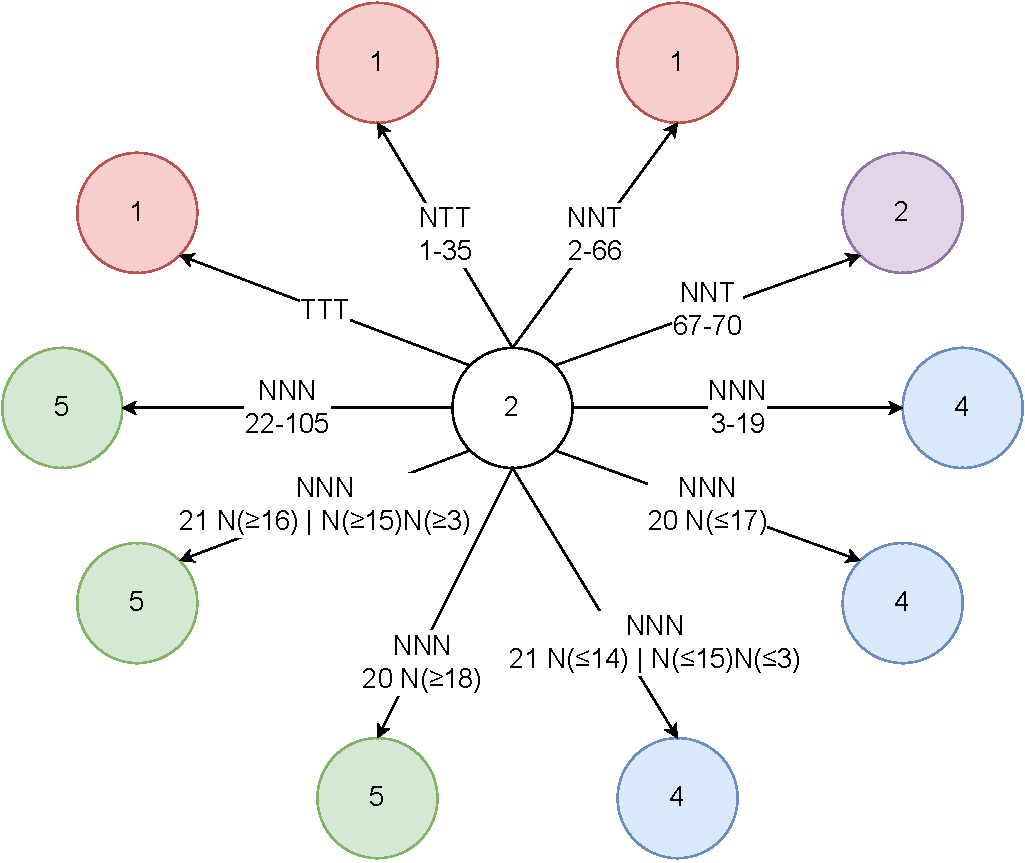
\includegraphics[width=\textwidth]{TITE-DTP-cohort3Node}
\end{figure}

\clearpage

\begin{figure}[h!]
	\centering
	\caption{TITE-DTP Flow plot for a cohort of two patients.}
	\label{fig_tite-dtp:TITEDTP-cohort3-flow}
	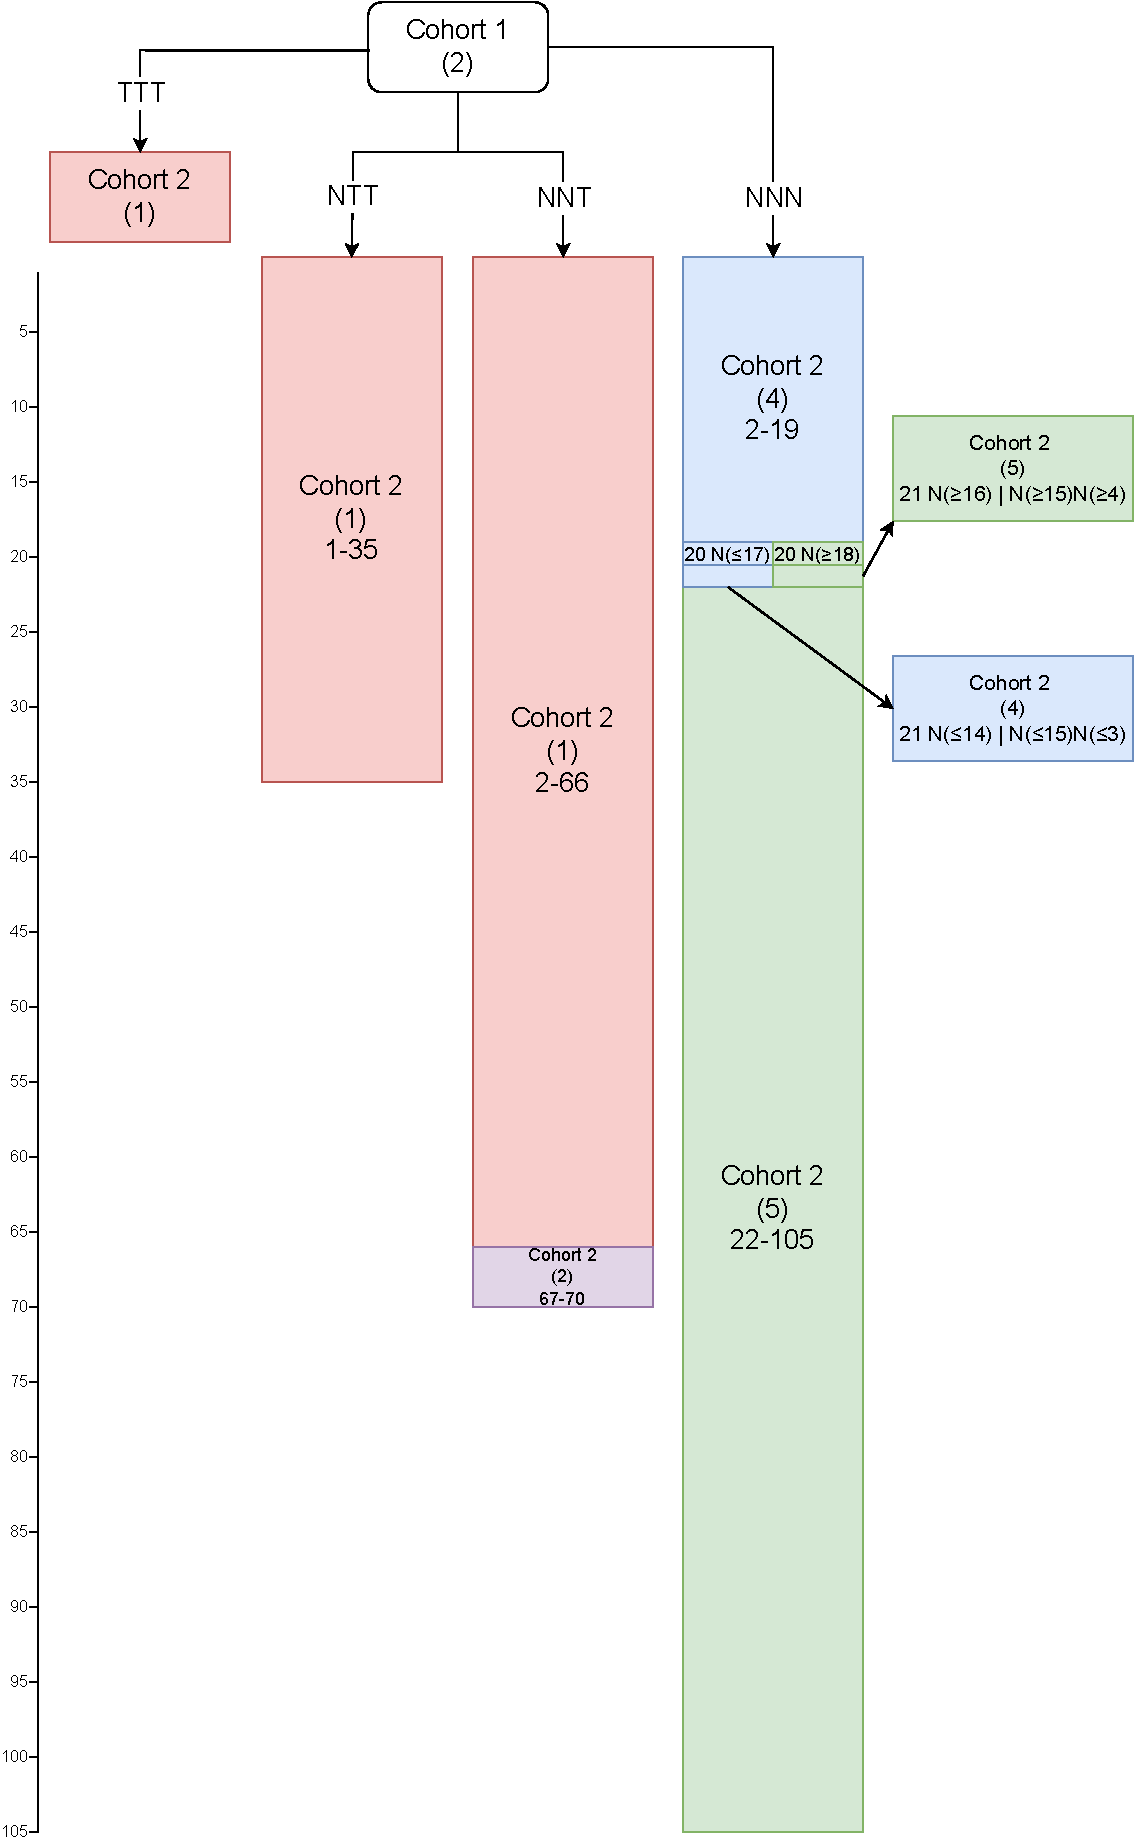
\includegraphics[height=0.93\textheight]{TITE-DTP-cohort3Flow}
\end{figure}

Back in section \ref{tite-dtp:UsingDTPs-Calibration}, we introduced a simple trial example and produced DTPs (Table \ref{tab_tite-dtp:InitialDTPExample}). The pathways for cohort 1 in that table are the full information equivalent of the TITE-DTPs in Table \ref{tab_tite-dtp:TITEDTP_c3_Sum}. As the same trial example was used to produce both of these pathways the only difference is for one of them we have allowed the ability to use partial information in the form of the TITE-CRM and introduce a follow-up period of 35 days. In Table \ref{tab_tite-dtp:InitialDTPExample} pathways 1-16 indicate NNN which is equivalent to Table \ref{tab_tite-dtp:TITEDTP_c3_Sum} outcome of NNN when the follow-up is max for each patient i.e. 105 days of combined follow-up. In both sets of pathways we can see the recommended dose for cohort 2 is dose-level 5. The outcome where all three patients have a toxicity is exactly the same for both the DTP and TITE-DTP. For the outcome of NTT we can see the recommended dose for cohort 2 is the same in both pathways, this implies allowing for partial information does not change the recommendation for this cohort. When we come to compare NNT we can see that allowing for partial information does have a slightly different impact on dose recommendations. If the cohort is evaluated when there are two partial tolerances with the number of combined follow-up days being 66 or lower the model recommends dose-level 1. Contrast this to when we have full information (each patient has 35 days of follow-up with no toxicity or just the CRM version of the DTP, Table \ref{tab_tite-dtp:InitialDTPExample}) and the recommended dose is 2. TITE-DTPs also allow you to compare your design to one with full information i.e the CRM equivalent of a TITE-CRM and allow you to evaluate the length of the follow-up period and see how the dose decisions change as you move through it. 

%----------------------------------------------------------------------------------------
%	SECTION 3
%----------------------------------------------------------------------------------------

\section{Discussion}
\label{tite-dtp:Discussion}

Dose transition pathways as a tool were developed to improve communication and understanding of model-based designs. Often clinicians may not feel comfortable with having a model select doses when compared to the standard approach of a traditional and easy to follow rule-based design \cite{jakiUptakeNovelStatistical2013}. DTPs try to bridge this gap and make these model-based designs more approachable. They do this by summarising model recommendations based on possible outcomes into simple pathways of dose decisions. They also can be used by the statistician to help calibrate the model and any design specifications. In particular, this helps with implementing stopping rules and investigating how escalation occurs. There is also a potential operational upside where DTPs can aid the running of a trial. By looking ahead there may be instances where regardless of any outcomes observed on the trial the dose-level will not change. In scenarios like this the need for a statistician may be lessened. 

DTPs can also be implemented as a visualisation tool to help visualise all the pathways in advance. This may have benefits in terms of raising any imminent safety concerns if certain pathways are followed. They can also be used throughout a trial's life cycle at safety committee meetings to discuss potential doses for future cohorts of patients. They are also very adaptive and are able to handle many challenging circumstances such as a change in cohort size or a patient receiving an incorrect dose. If these circumstances were to occur new DTPs could simply be calculated to account for any trial deviations. Although this is not an exclusive feature of DTPs, they are only capable of handling these scenarios because they can be accounted for in model-based designs like the CRM. 

A lot of this chapter focused on providing examples of how DTPs could be implemented specifically for a CRM design. However, the concept can easily be applied to many other model-based dose-finding trial designs such as BOIN and EffTox and even the 3+3. Implementation of these DTPs is relatively simple as well with the escalation package by Brock \cite{brockModularApproachDose2020}. It should be noted, as mentioned above, some of the flexibility of DTPs is due to the underlying designs that are used to make them. So, some challenges may be found when producing DTPs for certain types of trial designs. 

It is clear that the inclusion and use of DTPs is a net positive for dose-finding trials, not just in their design but also during the running of the trial. This is also reflected in guidance that is being published relating to the conduct and reporting of trials. Statistical Analysis Plan (SAP) guidelines produced by Gamble et al. \cite{gambleGuidelinesContentStatistical2017} in 2011 were extended by Homer et al. \cite{homerEarlyPhaseClinical2022} in 2022 to provide guidance for early phase trials. The authors here advocate for the use of DTPs where appropriate when producing SAPs for dose-finding trials. The DEFINE study \cite{solovyevaDevelopmentConsensusdrivenSPIRIT2023} aimed to extend the SPIRIT (Standard Protocol Items: Recommendations for Interventional Trials) 2013 statement \cite{chanSPIRIT2013Statement2013} and the CONSORT (CONsolidated Standards Of Reporting Trials) 2010 statement \cite{moherCONSORT2010Explanation2010} for use in early phase dose-finding trials. This led to the development of SPIRIT-DEFINE \cite{yapEnhancingQualityImpact2023} and CONSORT-DEFINE \cite{yapEnhancingReportingQuality2023}. Whilst SPIRIT-DEFINE explicitly include DTPs in their checklist they are not included in CONSORT-DEFINE. This makes sense as DTPs are more of a tool during the design and conduct of a trial and therefore more relevant to include in protocols. However, in scenarios where a dose-finding trial is stopped early, for issues other than safety, the reporting of these trials could also include DTPs to report what the potential results of the trial may have been. 

In the discussion section of the Yap et al. \cite{yapDoseTransitionPathways2017} paper which first introduces the idea, there is some mention of applying DTPs to TITE-CRMs. They mention the problems with patients having either partial or full tolerance and how DTPs may differ depending on how much follow-up time they achieve. One recommendation they gave was to produce the CRM equivalent DTPs. This would be useful during design stages to assess whether dose decisions change with full or partial information. 

Our work agrees with what Yap et al. \cite{yapDoseTransitionPathways2017} originally theorised. Extending DTPs to a TITE-CRM is problematic. Firstly, due to the idea of partial tolerances, trying to account for every possibility and time point a patient has not had a toxicity is an exponentially increasing problem. The complexity of DTPs is intrinsically linked to patients with partial tolerances as to fully build out the TITE-DTP you need to calculate every possible time point at which that patient could be observed. Then also for cohorts of more than one patient, considering the outcome where both patients experience a partial tolerance exponentially increases the number of pathways. We demonstrated that by showing the different potential DTPs for cohorts of patients from sizes one to two to three and how the number of pathways kept increasing with each iteration. 

We also found the TITE-CRM to have small inconsistencies when escalating doses. In some instances, different dose decisions were being made based on the split of follow-up time between patients for the same overall combined follow-up time. So, in our examples and TITE-DTPs for a cohort of two or three patients we saw different recommendations when the combined amount of follow-up time between the three patients was 20 and 21 days dependent on how those were split between the patients. We have shown this is dependent on the model parameter and that different combinations of follow-up times produce different estimates of the parameter due to the likelihood function. The model parameter $\beta$ can take any real value. As such there are specific boundaries or thresholds that exist at which the dose-decision will change dependent on the value of $\beta$. However, trying to strictly define these as a specific value is difficult as the way a dose is selected is based on the smallest difference between the estimated probability of toxicity at that dose and the target toxicity level. This difference can be infinitesimally small and as that tends to zero the value of $\beta$ which leads to that small difference tends to a specific boundary/threshold value. However, we can define a two values for $\beta$ at each adjoining dose-level to say a value above will result in the higher dose being recommended and a value below the other value will mean the lower dose is recommended.

Understanding this exact boundary is not paramount as in a practical setting due to the observation window or the number of patients you have you may not get close to that specific value of $\beta$ where the dose decision changes. As with our examples where values of $\beta$ below 0.1492 resulted in a dose-recommendation of dose-level 4 and any value above 0.1493 resulted in dose-level 5 being recommended. We saw this corresponded with combined follow-up times between 20 and 21 days. Understanding the exact combination of follow-up days for patients that lead to a dose decision is important to help us construct the TITE-DTPs. This is another advantage of DTPs in a TITE setting as they allow us to see exactly what amount of data we need to observe for specific decisions to be made. This may be helpful in practice when it comes to timing analyses for dose-decisions as it may be beneficial to observe patients for a few extra days in order to escalate to a higher doses. Whilst this may be a rare occurrence in an actual trial it will still be beneficial to be aware that his problem could arise and develop a plan ahead of time to deal with it. 

It is also important to note that this inconsistency may change how we intuitively interpret patients weighting in a TITE-CRM, specifically with a linear weight function. Through our examples we have shown that follow-up time between patients at the same dose-levels is not equally weighted. We saw that for the same combination of or total follow-up time different dose recommendations were made based on the split of follow-up time between the patients. Even in instances where different dose-recommendations were not made we still saw different estimates of $\beta$ for different combinations of the same total. Even with the linear weights it is the non-linearity of the weights that causes this problem. An extensive review of the literature has not been conducted however we do not think that this issue with the TITE-CRM has been highlighted previously, this may also extend to other methodology which implements a TITE component. 

Further work may be done to explore this issue and the idea of TITE-DTPs. Here we have only looked at a relatively simple example using a TITE-CRM with a power model and a linear weight function. A more complex weight function could further highlight this issue such as the adaptive weight function presented by Cheung and Chappel \cite{cheungSequentialDesignsPhase2000}, Huang and Kuan \cite{huangTimetoeventContinualReassessment2014}, or Braun \cite{braunGeneralizingTITECRMAdapt2006}. For example if more weight is given to patients early in the observation window, the effect we observed in our example may be further exaggerated. Our example design was not a modified TITE-CRM so we did not make use of any stopping rules or rules about skipping doses. Changes to any of the specifications or the inclusion of these rules would alter the results we produced. It is also possible that this issue may be less apparent in the early stages of a modified TITE-CRM example. If a rule was included to avoid skipping doses the initial set of doses the TITE-CRM could explore would be restricted. However at a certain point once multiple dose-levels had been tested the issue may reappear.

Additionally, the observation window of 35 days that we selected was also fairly arbitrary and as discussed previously any significant increase in this value will drastically increase the number of pathways that need to be calculated. We only looked at patients at the start of the trial all of whom received the same dose-level. An additional approach would be to look at the pathways halfway through the trial assuming previous patients had been fully observed so we would not have to consider multiple pathways from that data. Looking into a more complex example and multiple scenarios to see if TITE-DTPs still behave as we have described would be beneficial to validate the work we have already done as well as highlight any different features that may emerge such as the inconsistency with weighting that we found.

The examples of TITE-DTPs we provided were for only one cohort as well. Obviously, this becomes more and more difficult to deal with as we add in extra patients and cohorts. It is also not as trivial as just presenting a summary table as we did for the first cohort as well. Any additional cohort will have to take into account not only partial tolerance events from the new cohort but would have to consider every remaining possible partial tolerance event from a previous cohort. Consider one pathway from a cohort of three, N(31)N(23)N(9), all patients here experienced a partial tolerance and as their combined follow-up time adds up to 63 days we can see from the TITE-DTP in Table \ref{tab_tite-dtp:TITEDTP_c3_Sum} the dose recommendation would be dose-level 5. If we were to then recruit cohort 2 to dose-level 5 and attempt to produce more pathways we would need to check combinations for each possible amount of remaining follow-up time for the patients in the previous cohort as well as the full 35 days for each of the three new patients. So, this can essentially be thought of as a cohort of six, where some patients already have some data available. Equation \ref{eq_tite-dtp:combinations} can then be used to give us a rough estimate of how many combinations need to be considered. For a cohort of 6 patients with 35 days of follow-up, the number of combinations is $1 \times 10^{41}$. Now since we already have some data a few of these combinations are redundant but that is still an astronomical amount of pathways. For context the universe is approximated to be 13.7 billion years old \cite{DictionaryPhysics2009} which roughly converts to $4.3 \times 10^{17}$ seconds i.e. there are more possible combinations than there are seconds that have passed since the beginning of time. 

The TITE-CRM was originally designed to work without the use of cohorts. The idea was that patients could be recruited into the trial continually and they would be allocated a dose-level based on data from patients already in the trial. As those patients already in the trial may not have completed their DLT observation window they would be partially weighted using the idea of them having achieved a partial tolerance. As recruitment to a clinical trial may not be consistent or predictable this made it possible to not pause recruitment in a dose-finding trial which would typically be done whilst a cohort was being observed for DLTs. However, in a practical setting and with guidance from regulators it may not always be possible to run trials in this manner. In order to make a dose-decision data may have to be source verified and cleaned. A report and analysis will have to be produced and  used to make a dose-decision which is then discussed with an independent committee. This process may take weeks and recruitment may have to be paused to allow for this to occur before the next patient is recruited. Werkhoven et al. \cite{vanwerkhovenPracticalitiesRunningEarlyphase2020} provide a full discussion on the practicalities of running a TITE-CRM and the challenges it raises. However, the TITE-CRM still remains useful as we can have long observation windows to monitor late-onset toxicities and still make dose-decisions whilst observing patients (Like we have done in Chapter \ref{Adept} for the ADePT-DDR trial). As such TITE-DTPs can still be a useful tool.

One way in which TITE-DTPs could work with multiple cohorts would be if previous cohorts were completed and had full information. That data could go directly into the model and you would not need to consider any previous partial tolerances. When a dose decision for cohort 2 is made on partial information from cohort 1, TITE-DTPs could be created showing outcomes for cohort 3 that assume cohort 1 has full information. In practice, this may very much be the case as well depending on factors such as recruitment time and the follow-up period. 

The way DTPs are calculated the outcomes are specified and then entered into the model and then the recommended dose based on those is extracted. Those values are then used to construct the DTPs. That means for each outcome we have to specify an individual model. So, earlier in the chapter when there were 64 pathways 64 models were fitted and in the example of TITE-DTPs for a cohort of 3 we had 8436. As you increase the cohort size and the number of patients or the number of follow-up days in the trial, the number of pathways increases hence the number of models required to compute the DTP increase and the more models required the more computing time is needed. One way around this may be to stop computing once a dose-decision threshold is reached. This specifically relates to any outcomes where a partial tolerance occurs.  In the TITE-DTP example for the NNN outcome, we see anything after 27 days of combined follow-up recommends dose-level 5, We could incorporate a rule into our code that checks after each combination of follow-up days if the recommended dose changes and remains the same across every permutation of follow-up time across the patients DTPs would stop being calculated and you can assume the recommended dose will be the same. That is to say in this scenario for every combination of the three patients' follow-up time that adds up to 27 the model recommends dose-level 5 so we can assume that for any additional follow-up time the model will make the same recommendation as that is the maximum dose. This could cut down computing time on thousands of additional pathways depending on the scenario and context. 

An alternative method of producing TITE-DTPs may be to use patients' weight as a reference instead of their follow-up time. Even though weight is a function of follow-up time it might make presenting the TITE-DTPs simpler. A set of weights could be specified and pathways for those could be calculated instead. So rather than calculating pathways for N(1), N(2), ..., N(34), N you just calculate pathways when a patient is at 25\%, 50\%, 75\% and 100\% weighting. The issue with this is in order to make it interpretable you would have to back-transform the weighting. So in our example with a 35 day follow-up period and a linear weight function weightings of 25\%, 50\%, 75\% and 100\% would correspond to 8.75, 17.5, 26.25, and 35 days respectively. This might not be intuitive but it is one way to reduce the number of potential pathways. For cohorts of two or more where multiple patients are experiencing partial tolerance rather than looking at every possible combination you could just look at specific weightings. For example what is the pathway when both patients are at 50\% weight, or perhaps when one is at 75\% and the other at 25\%.  

As Yap et al. \cite{yapDoseTransitionPathways2017} suggested perhaps the easiest approach is just to assume that full tolerance will be achieved and calculate DTPs from that viewpoint. So treat the trial like a CRM and give full weighting to all the patients. This could be used as an alternative and a way to compare dose decisions made on partial information versus full information. This comparison was also made in our example and we saw how some decisions may change with only partial information. During the design stage of a trial, this may be useful in helping determine the length of any potential observation window and how dose decisions may change during it.  

Overall it is possible to produce TITE-DTPs but it heavily depends on the number of days that patients can have a partial tolerance. It also depends on the size of the cohort you are evaluating. There are also some practical suggestions for how TITE-DTPs could be used during a trials design as well as it is running. Based on all these factors it appears problematic to produce TITE-DTPs for more than one cohort at a time and this will only be feasible during a trial if you can assume complete information on previous cohorts. Ultimately TITE-DTPs are still able to achieve the same aims as DTP except its ability to look ahead is a lot less. Statisticians should attempt to produce them wherever possible. However, if the scenario or trial parameters mean the TITE-DTPs is too complicated they may be more of a hindrance than a benefit.
% Chapter Template

\chapter{Efficacy Transition Pathways} % Main chapter title

\label{etp} % For referencing this chapter elsewhere, use \ref{etp}

%----------------------------------------------------------------------------------------
%	SECTION 1
%----------------------------------------------------------------------------------------

\section{Introduction}
\label{etp:Introduction}

In Phase \RN{2} trials we are often attempting to determine whether or not a new treatment or intervention works and establish if there is a efficacy signal. More specifically they aim to determine if there is sufficient level of evidence to warrant further research in a Phase \RN{3} setting. In addition to assessing efficacy there is also opportunity to further explore the toxicity profile of the treatment compared to Phase \RN{1} trials Phase \RN{2} trials are typically conducted using a larger sample size. Generally speaking Phase \RN{2} trials should be efficient and quick such that we can progress to Phase \RN{3} as quickly as possible or drop any ineffective treatments.

The output from a Phase \RN{2} trial should be either a 'GO' or 'No GO' decision i.e should we or should we not proceed to later phase testing based on the data observed in this trial. One of the more important aspects of these trials is that we don't want to make any incorrect decisions and if there is an effective treatment that is being investigated we want to make sure that it is taken forward into Phase \RN{3}. As such it is important that we try to make correct decisions in Phase \RN{2} trials. Failure to do so could result in potentially beneficial treatments being rejected or bad treatments being investigated further, which could negatively impact patients and waste a lot of time and money. 

However, Phase \RN{2} trials still face some issues which may make this challenging. Whilst it is the case that Phase \RN{2} trials are typically larger than Phase \RN{1} trials there are still some instances in which we would be dealing with small sample sizes. For example, in a rare disease setting. In these instances we may employ single arm Phase \RN{2} trial designs along with Bayesian methods to make better use of the data we are able to collect. 

Furthermore, we may also be interested in taking a look at the data more frequently to ensure the treatment is adequately safe and if there is some signal of efficacy to warrant continuing the trial. This may take the form of interim analyses and can be thought of in a similar manner to dose decisions in dose-finding trials. Rather than assessing the data and selecting a dose we are assessing if the trial should continue or not, stopping for either futility or safety reasons.  

Whilst these designs may be simple to implement they also suffer from similar drawbacks as certain dose-finding methodologies, that have previously been discussed. There may be some issues parametrising these designs e.g. selecting adequate decision rules. Any Bayesian approaches may be less familiar than traditional frequentist approaches that are more commonly used. Clinicians and non-statisticians may struggle to understand why certain decisions are being made during interim and final analyses. 

In order to solve some of these issues Lucinda Billingham (LB) developed Efficacy Transition Pathways (ETPs) a novel visualisation tool to aid the design and interpretation of these types of designs. ETPs are an extension on the idea of Dose Transition Pathways (DTPs). Here they help map out and visualise the different decisions that can be made at interim and final analyses based on different observed outcomes in a similar manner as how DTPs present different dose-decisions that can be made for each cohort. 

In this chapter we will detail how ETPs are constructed as well as how they may be used in practice. In addition we present motivating examples where ETPs have been actively implemented and used in clinical trials. Finally we detail a web application that was developed to facilitate production of ETPs and act as an education tool to explain what they are and their purpose. 

%----------------------------------------------------------------------------------------
%	SECTION 2
%----------------------------------------------------------------------------------------

\section{Efficacy Transition Pathways}
\label{etp:ETPs}

ETPs were primarily designed for use in single arm Phase \RN{2} trials using Bayesian methods where the data is being looked at and assessed frequently. Typically a trial like this, at least in an oncology setting, will have a short-term binary outcome either success or failure, response or no response as its primary outcome. 

One approach for these sorts of trials is to use a Beta-Binomial conjugate analysis to estimate a response rate for the binary outcome. Posterior probabilities can be used to inform decision making and predictive probabilities can be used during interim analyses in a similar manner. Any decisions made will be done using pre-specified decision rules.

In order to demonstrate how ETPs are constructed and used we will look at the design process for a trial using a Beta-Binomial conjugate analysis. When implementing a design like this we need to consider a number of factors such as: the total sample size, the number and timing of any interim analyses, and decision criteria for interim and final analyses. Then much like with a dose-finding trial simulations can be conducted to obtain operating characteristics of the design. In addition we can also calculate the number of responses required at each analysis to continue the trial. This is also an iterative process so the design and decision rules can then be tweaked until an acceptable design is reached. 

ETPs can be utilised during this process as they are able to present the decisions that will be made based on the current design specification and the potential outcomes that can be observed for each analysis time point. As the design process for a trial involves multiple stakeholders it may not be easy to understand why or when certain decisions are being made. By mapping this all out in a single plot it may be easier to visualise. 

For example, based on whatever the current specification is, it may be the case that in the first interim analysis 2/5 patients require a response to continue the trial. Once the clinicians see this they may feel its too strict and would only think about stopping if there are no responses or alternatively they may want to remove this interim analysis and decide to only look at the data once 10 patients have been recruited. This is far more intuitive then trying to explain these concepts and using different boundaries for predictive probabilities. This could then be used to facilitate further discussions about the design specification and if decision rules need to be more or less lenient.  

ETPs much like DTPs could also be used throughout the trial as well. So, based on how many responses have already been observed you can easily figure out how many responses would be required for the next cohort of patients to obtain a 'GO' decision. Once the ETPs are produced all future decisions based on the number of responses can also be seen. So, this has the benefit of not requiring a statistician to run an analysis every time you need to figure out how many more responses are required for a 'GO' or 'No GO' decision. Whilst, ETPs should not replace the need for a statistician and they should still be involved with all the analyses they act as a tool that can help monitor the progress of a trial and can be referred to throughout the trials life cycle. In the next sections we provide an example trial to show how ETPs are constructed and utilised. 

%-----------------------------------
%	SUBSECTION 1
%-----------------------------------

\subsection{Illustrative example to showcase a Beta-Binomial design} 
\label{etp:BBIllEx}

Consider a Phase \RN{2} trial in which we are trying to evaluate the efficacy of some new treatment.This will be done using an outcome measure of response. Patients can either be considered a responder or a non-responder. Lets assume this is in a rare disease setting so patient numbers are limited and as such we will be using a single-arm design. The treatment effect will be the response rate and will be analysed using a Beta-Binomial conjugate model. We will require a sufficient level of evidence that the there is adequate treatment effect to warrant further research in a Phase \RN{3} trial.

To conduct the analysis and make a GO or No GO decision a prior and decision criteria need to be specified. For simplicity a minimally informative Beta(1,1) prior will be used. This represents a 50\% response rate from a group of two patients. Data will also need to be collected from patients recording if they had a response or not. This in turn is combined with the prior distribution to generate a posterior distribution for the treatment effect. Then pre-specified rules based on these direct probabilities from the posterior can be used for decision making purposes. This can take the form of

\begin{equation}
	\label{eq_etp:betafinaldecrule}
	P(\theta > c |y) \geq q  \; \; \; \; \text{then GO else No GO}
\end{equation}

where $\theta$ is the treatment effect (response rate), $c$ is some target level of treatment effect (target response rate), $y$ represents our data and $q$ is some threshold of sufficient evidence (acceptable probability level). 
 
For our example the following decision rule will also be used $P(\theta  \geq 30\%) \geq 0.9$. So, if there is a greater than  90\% chance that the true response rate is at least 30\% this will be considered sufficient evidence to warrant a GO decision. We will also include interim analyses after every five patients to evaluate whether or not the trial should be stopped for futility. To do this we will use the predictive probability of success (PPoS).

This works by evaluating the data at pre-specified time points or after a certain number of patients have been recruited, in this example after every five patients. At these time points we can determine whether or not we have observed enough responses to warrant continuing with the trial based on the overall minimum responses we would need for a final GO decision. More explicitly the PPoS is the probability of the trial being considered a success given the current data observed at the interim analysis. This is calculated by predicting the future number of responses in the patients yet to be recruited based on the data that has already been observed and the prior distribution.

For our example trial we will specify a PPoS acceptable probability threshold where if PPoS < 0.05 then we should stop the trial for futility. This implies we would stop the trial if there is a less than 5\% chance that the response rate at the end of the trial will be greater than 30\% with a probability of 0.9 i.e a less than 5\% chance that the trial would reach a GO decision or be considered a success. 

Table \ref{tab_etp:exampleBBspecs} details the minimum number of responses required under this design at each analysis time point. For the final analysis, once 30 patients have been recruited, a minimum of 13 responses must be observed in order to have a GO decision. We can also see what the minimum number of responses required are for each interim analysis.

\begin{table}[h!]
	\centering
	\caption{Specification of parameters for the example Beta-Binomial trial.}
	\label{tab_etp:exampleBBspecs}
	\begin{tabular}{l|c}
		\hline
		\textbf{Analysis}     & \textbf{Minimum No. Responses for GO Decision}               \\ \hline
		N = 5  & 1                            \\
		N = 10 & 2                            \\
		N = 15 & 3                           \\
		N = 20 & 7                            \\
		N = 25 & 9                         \\
		N = 30 & 13                  \\ \hline
	\end{tabular}
\end{table}

Most of the specifications we have made here along with our decision rules are fairly arbitrary. In practice decision rules should be decided before the trial starts. This is typically done via the evaluation of simulations and looking at the minimum number of responses required for GO decisions. Multiple scenarios corresponding to different true response rates can be investigated. The probability of making a correct decision can then be calculated. This represents the power of our design. For scenarios with low true response rates (relative to the target response rate) we want the probability of making a No GO decision to be high. Similarly, for scenarios with high true response rates we want the probability of making a GO decision to be high. The decision rule parameters, the target response rate and probability threshold can then be adjusted to ensure the design is making appropriate decisions in these scenarios. 	

Whilst simulations are useful they may not convey what is most meaningful for other collaborators when assessing the merits of each iterative design specification. This is where ETPs can be used to try and bridge that gap by offering a way to visually represent key information and decisions that are made with these types of designs. In the next section we detail how an ETP is constructed using the example trial design specified here. 


%-----------------------------------
%	SUBSECTION 2
%-----------------------------------

\subsection{Constructing Efficacy Transition Pathways} 
\label{etp:conETPs}

At each interim analysis PPoS is calculated based on the number of responses observed thus far and evaluated to see if it meets the decision criteria. Therefore there will be a minimum number of responses that have to be observed in order to continue recruitment. This is similar to how we can calculate the number of responses required at the end of the trial to warrant a GO decision. Obviously, the minimum number of responses required at each interim and the final analysis depends on the decision criteria that is specified. 

Intuitively, it is easier to understand that three responses have to be observed from 15 patients rather than a PPoS $\leq 0.05$ is needed. Through discussions with clinicians we can then calibrate our decision criteria based on these interpretations. We may want to be more strict or lenient at our interim. If the clinicians would be happy to continue recruitment after seeing only two responses we could lower the PPoS threshold, likewise if they wanted to be confident and only continue if six responses were observed we would increase the PPoS threshold. Similarly, this can also be done for the final analysis decision criteria. The acceptable probability level or target response rate could be adjusted so a specific minimum number of responses observed achieves a GO decision. Obviously any changes made should be assessed by simulations as well, drastically changing the decision criteria could have a negative impact on performance. 
 
As you add more interims to a design like this trying to understand the break points at each interim become more complex. A solution for this is ETPs. In our example trial we have a maximum sample size of 30 patients with interim analyses planned after every five patients. This results in a total of six analyses, one final analysis and five interims. The decision criteria at the end of the trial requires the treatment effect to be greater than 30\% with a probability of 0.9 and to pass the interim analyses we require the PPoS to be greater than 0.05. 

To construct an ETP we produce individual cells which contain key information about a specific outcome i.e. a certain amount of responses. If we consider our first interim at five patients, at that point there are six different possible outcomes that can be observed. Either one, two, three, four or all five of the patients had a response or none of them did. For each possible outcome we can then calculate the PPoS as well as the Bayesian estimate of the response rate and an associated credible interval. Figure \ref{fig_etp:Cell0Resp5Pat} shows what this cell would look like. 

\begin{figure}[h!]
	\centering
	\caption{ETP cell plot for 0 responses in 5 patients.}
	\label{fig_etp:Cell0Resp5Pat}
	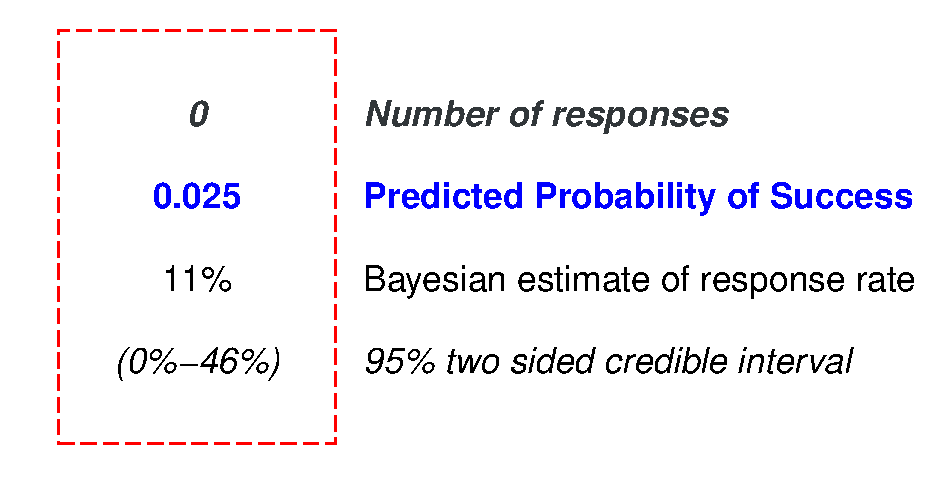
\includegraphics[width=\textwidth]{ETP-cell0Resp5Pat}
\end{figure}

The number at the top indicates the outcome for the cell, in this case the number of responses which is 0. The second row shows the PPoS in this scenario, the third row showing the Bayesian estimate of response rate and the last row shows the 95\% credible interval. For 0 responses the PPoS is 0.025 which is less than our threshold so the decision here would be to stop. This is represented by the red dashed line. From this one cell we are able to see what the decision would be at the interim analysis time point if this is the outcome that is observed. We are also able to see specifically what the PPoS and estimated response rate would be as well. The choice was made to present probabilities with decimals and any estimates of response rates with percentages. This was so the two could easily be differentiated and if you wanted to make a comment about the treatment effect we could directly look at the percentages and see the estimate and credible interval.   

Cells are generated for each possible outcome at each interim time point. Figure \ref{fig_etp:Cell2Resp5Pat} shows the cell for two responses in five patients. Here we can see the PPoS is 0.501 which is greater than our threshold so the decision would be made to continue recruitment. This is indicated by the green dashed line. As we put each cell together we can then clearly see the minimum number of responses required to continue recruiting.  

\begin{figure}[h!]
	\centering
	\caption{ETP cell plot for 2 responses in 5 patients.}
	\label{fig_etp:Cell2Resp5Pat}
	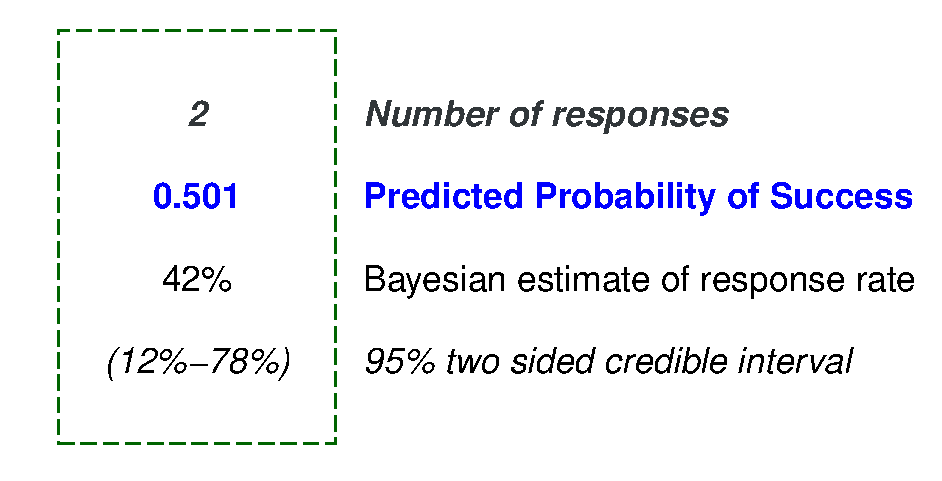
\includegraphics[width=\textwidth]{ETP-cell2Resp5Pat}
\end{figure}

This process is then repeated for each interim analysis. So, the next analysis would be at 10 patients. Here we would generate 11 cells for all the different possible outcomes (no response, one response, two responses, ..., 10 responses). The same would then be done for the analysis at 15, 20 and 25 patients. 

For the final analysis the presentation of the cells is slightly different. Here we are no longer interested in PPoS as no more patients will be recruited and rather we can just evaluate if the trial has met the decision criteria. So, in each cell rather than present PPoS the posterior probability that the response rate is greater than our target rate is presented instead. Figures \ref{fig_etp:Cell10Resp30Pat} and \ref{fig_etp:Cell14Resp30Pat} show the cells for 10 responses and 14 responses out of 30 patients respectively. In this example our $q$ is set at 0.9 so if the posterior probability is greater than that we have a GO decision. 

\begin{figure}[h!]
	\centering
	\caption{ETP cell plot for 10 responses in 30 patients.}
	\label{fig_etp:Cell10Resp30Pat}
	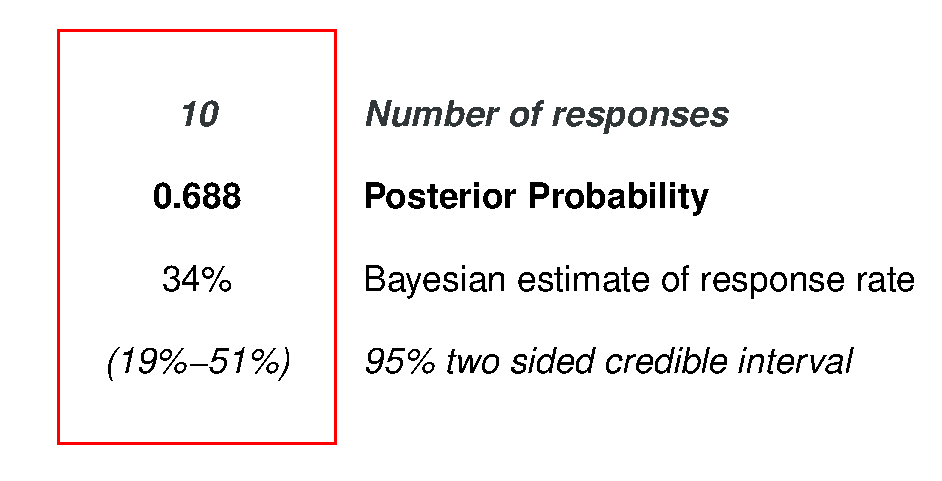
\includegraphics[width=\textwidth]{ETP-cell10Resp30Pat}
\end{figure}


\begin{figure}[h!]
	\centering
	\caption{ETP cell plot for 14 responses in 30 patients.}
	\label{fig_etp:Cell14Resp30Pat}
	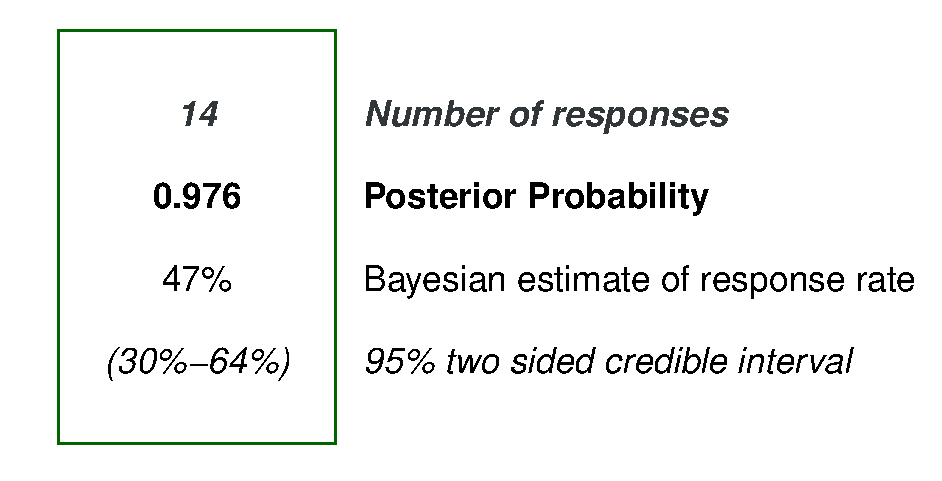
\includegraphics[width=\textwidth]{ETP-cell14Resp30Pat}
\end{figure}


The efficacy transition pathway is then constructed by grouping each cell for each interim analysis and then stacking those group of cells together. For our example trial the ETP is shown in Figure \ref{fig_etp:ConstructedETP}. Each row of cells in the ETP represents each interim analysis with the final row representing the final analysis. One adaptation made with the cells is that the confidence interval is presented across the bottom two rows in each cell just to make the figure easier to read and more scalable. 

From this figure what can clearly be seen is when we do or do not have a GO decision. At each interim of 5, 10, 15, 20, 25 patients we can see that the minimum number of responses for a GO decision is 1, 2, 4, 7 and 9 respectively. Also, for the final analysis a minimum of 13 responses is required. We can also read down the figure to gauge an idea of how many additional responses would be required in future analyses to warrant a GO decision. For instance if you observed five responses in your first cohort of five patients, that is enough observed data to continue passing the interim decision criteria until the fourth interim analysis in which case you would need an additional two responses. This can easily be seen by reformatting the ETP to be aligned to the left so the same number of responses are stacked on top of each other for each cohort. This is illustrated in Figure \ref{fig_etp:ConstructedETPleft}. 

In addition to the easy visualisation of the number of responses required to achieve a GO decision we can also quite easily see the estimates of the treatment effect for each potential outcome and each analysis time point. This is useful for interpreting the results for the final analysis (the bottom row of the ETP plot). Right away from interpreting the cell for the minimum number of responses (13/30) for a GO decision we can see the estimated response rate would be 44\% with a probability of 0.95 that the true response rate is between 27\% and 61\%. We also need to keep in mind the original decision rule for the final analysis which for any GO decision implies there is a greater than 0.9 probability that the response rate is greater than 30\%. This can then be used to facilitate discussions with the clinicians to deem if this is an acceptable level of evidence to warrant further research or potentially bring into practice, based on previous studies, current treatments or their experience. We can then adjust our design and decision rules accordingly, which we discuss in the next section. 

\begin{sidewaysfigure}
	\centering
	\caption{Example of a constructed ETP.}
	\label{fig_etp:ConstructedETP}
	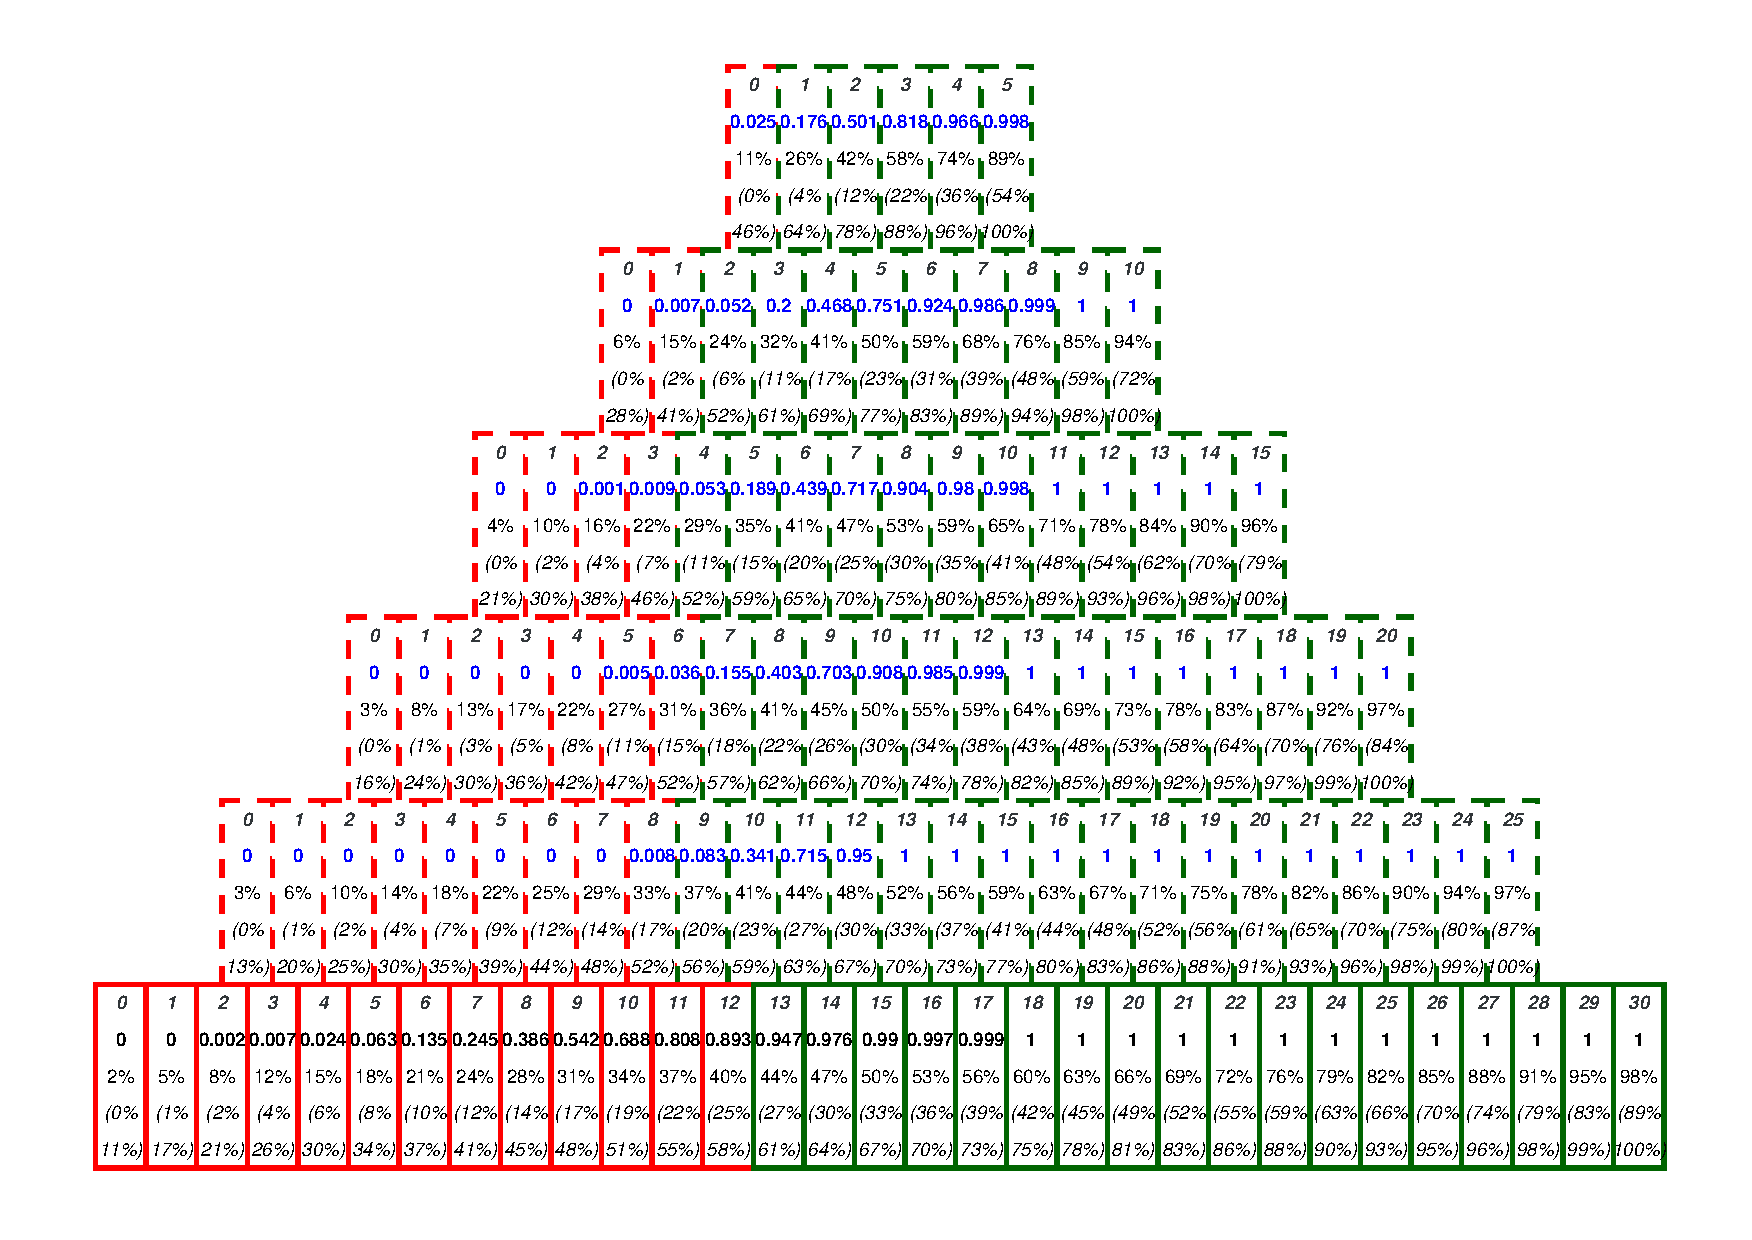
\includegraphics[width=25cm, height=15cm]{ETP-constructed}
\end{sidewaysfigure}

\begin{sidewaysfigure}
	\centering
	\caption{A left aligned version of the constructed ETP.}
	\label{fig_etp:ConstructedETPleft}
	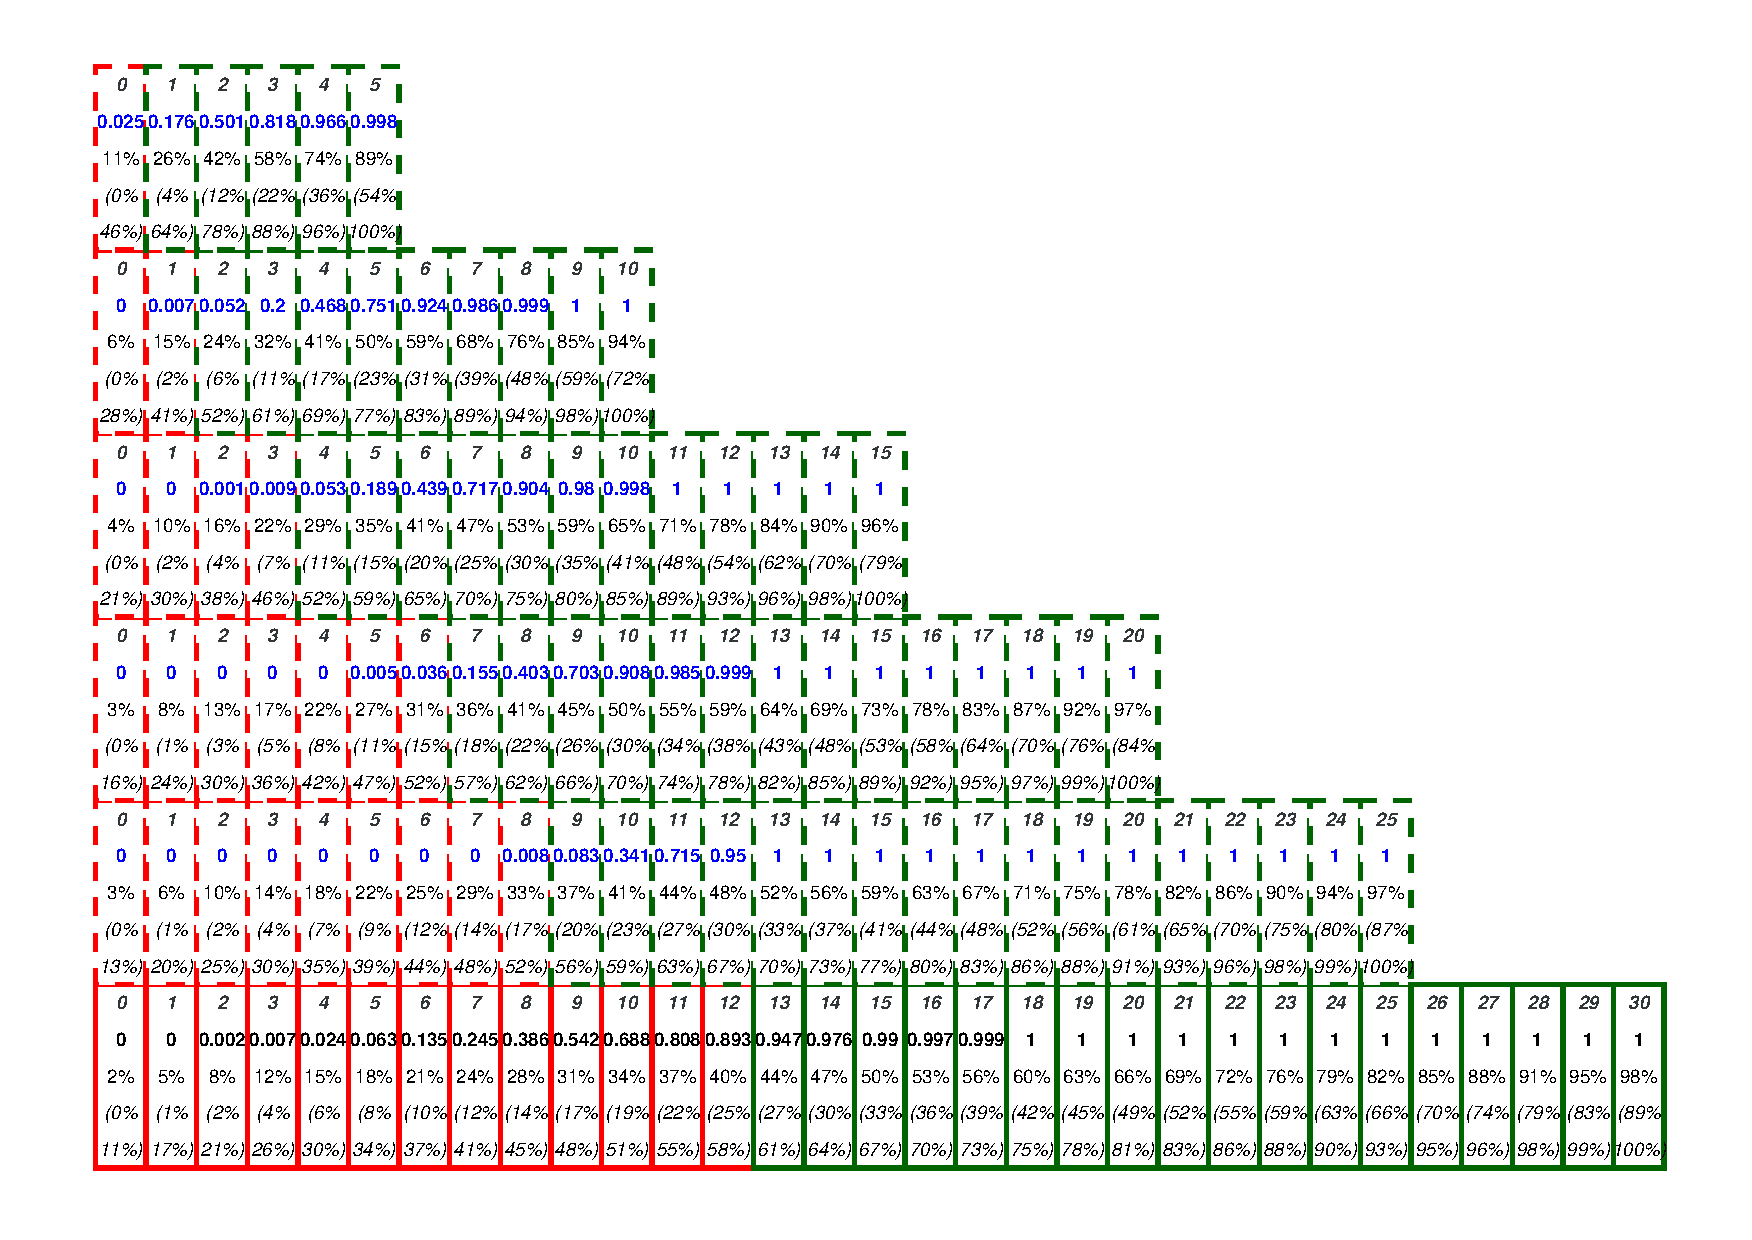
\includegraphics[width=25cm, height=15cm]{ETP-constructedleft}
\end{sidewaysfigure}

\newpage
%-----------------------------------
%	SUBSECTION 3
%-----------------------------------

\subsection{Updating decision criteria based on Efficacy Transition Pathways} 
\label{etp:updatingETPs}

Having seen the ETP we created for our example trial, suppose we want to modify our decision criteria such that a GO decision at the final analysis requires only nine patients to achieve a response. Compared to the initial decision criteria, which required 13 responses, we may want to  consider lowering this due to the treatment options available for these patients may not being very effective. Obviously there may be many reasons why we would want to increase or decrease this requirement and this would depend on the context and background of each individual trial. This is just to provide an illustrative example of why we might consider changing the criteria and how we go about it with ETPs. 

By looking directly at the ETP Figures \ref{fig_etp:ConstructedETP} or \ref{fig_etp:ConstructedETPleft} we can see that nine responses out of 30 patients has a posterior probability of 0.542. So, based of the initial decision rule of $P(\theta  \geq 30\%) \geq 0.9$, this implies that the probability that the response rate is greater than or equal to 30\% is 0.542. Therefore, if we wanted to make this a GO decision we would change our decision criteria such that our acceptable level of probability was something smaller than that posterior probability. For example, a new decision rule could be $P(\theta  \geq 30\%) \geq 0.5$ this would mean that nine responses out of 30 patients would now be a GO decision. This is another benefit of ETPs, we can quickly ascertain how we would need to change our decision criteria to be in order for a specific minimum number of responses to be a GO decision. 

Let's say we implement that new decision rule, we can then create an updated ETP. In Figure \ref{fig_etp:ConstructedETP_30-50_5} we can see for the final analysis (the bottom row of the plot) GO decisions start from nine responses. It is important to note the content of these cells haven't changed. The estimates of response rates and credible intervals are still the same. This is because we fundamentally haven't made any changes to the design just the criteria for which we are making decisions. Changes in these estimates would only be triggered if we were to change the total sample size. Additionally the posterior probabilities are also consistent with the previous ETP, this is because we haven't altered the targeted response rate in our decision criteria. This value is still showing the probability that the treatment has a response rate greater than 30\%. These values would only differ if our target response rate was set as something else. For the rest of the cells showing previous cohorts and the interim analyses we can see the minimum number of responses required for a GO decision is now 0, 1, 3, 4 and 6 for each interim analysis respectively. Also, note how the PPoS is different compared to the last ETP this is because PPoS takes into account the final decision rule we are using. Any change to that rule will impact PPoS calculations. 

\begin{sidewaysfigure}
	\centering
	\caption{ETP with updated final decision rule.}
	\label{fig_etp:ConstructedETP_30-50_5}
	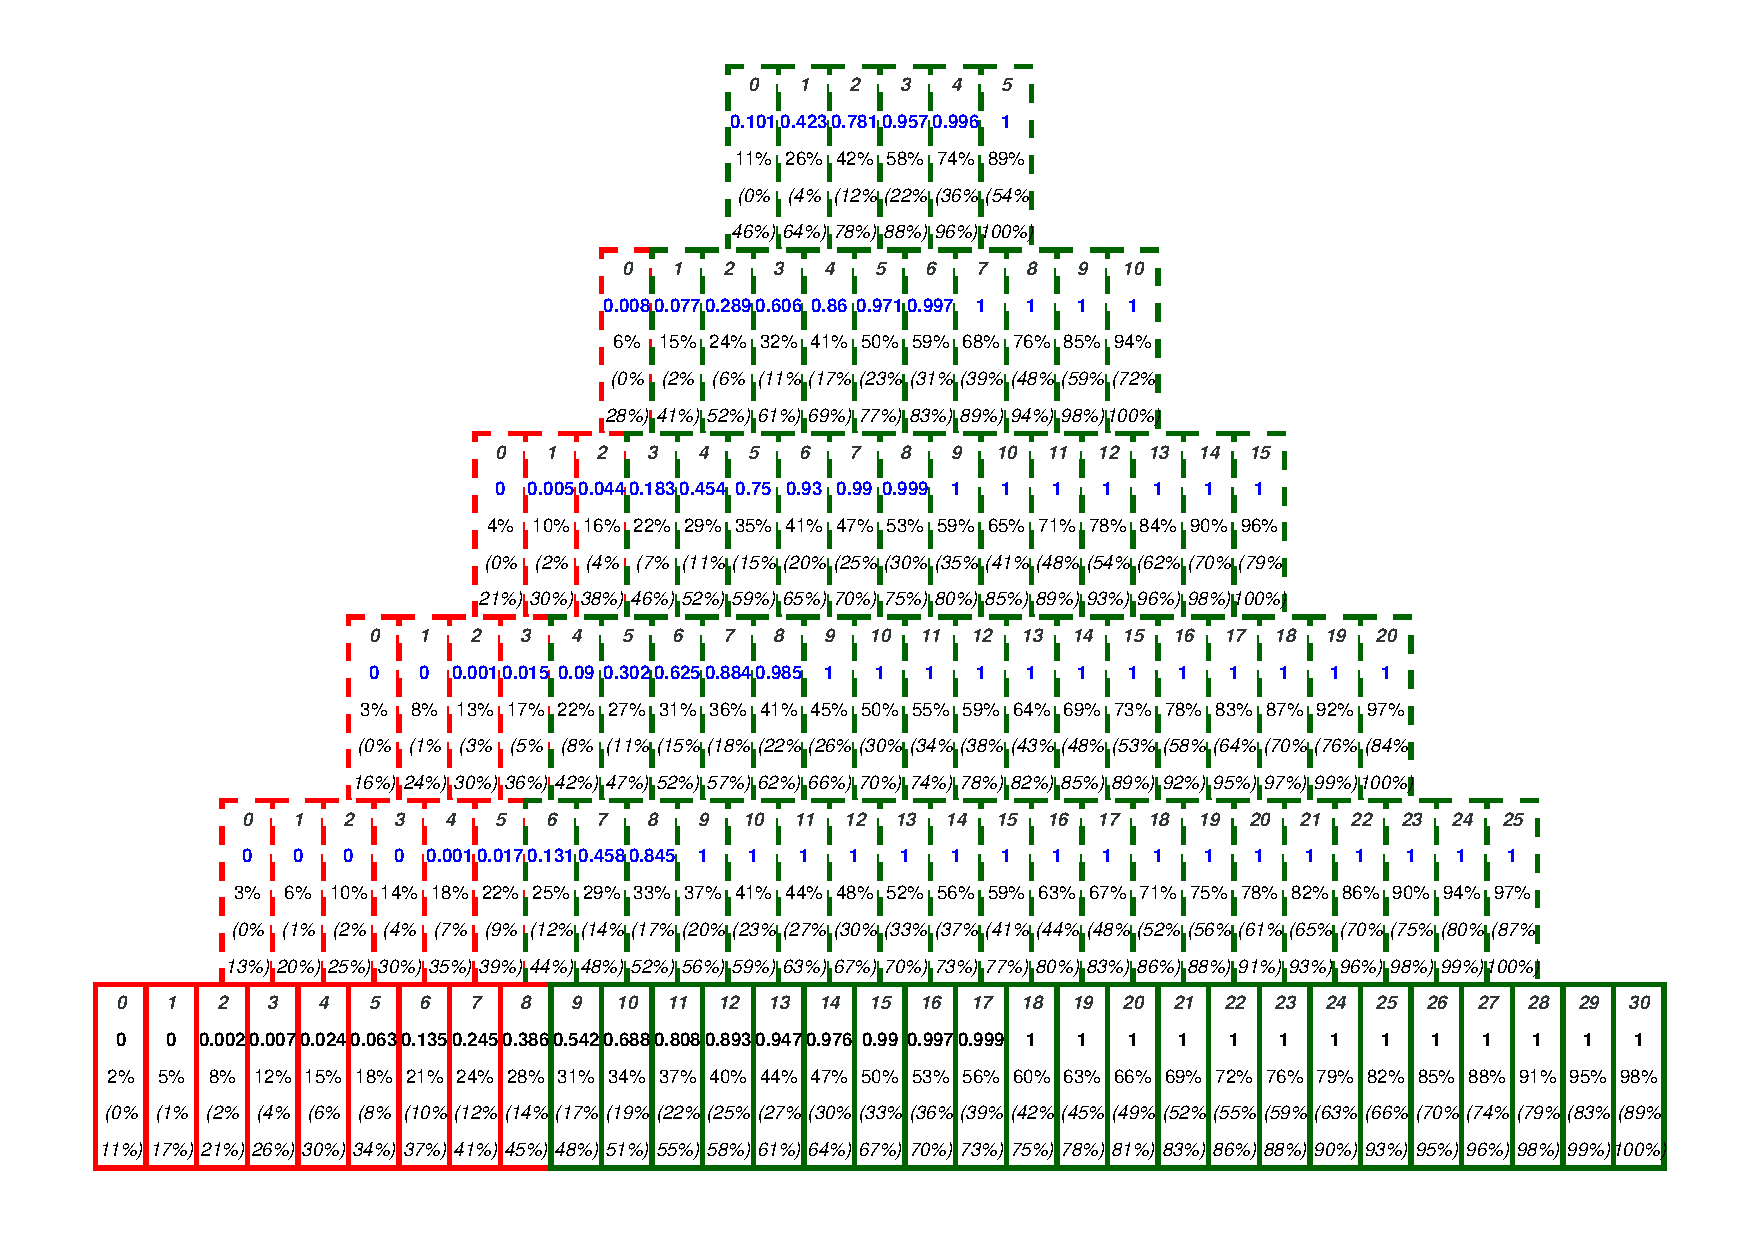
\includegraphics[width=25cm, height=15cm]{ETP-constructed_30-50_5}
\end{sidewaysfigure}

By altering our decision rule like this we ensure that if we observe the desired number of responses, in this case nine, the trial would be a success. We did this by just changing $q$, the acceptable probability level. However, it should be noted that this can also be achieved by changing both $c$ (the target response rate) and $q$. These values can both be manipulated so we still maintain the same practical decision making. This is important to note as whilst clinicians may find it more intuitive to specify decision rules based on a minimum number of responses there are different ways in which that can be achieved. 

Table \ref{tab_etp:DecisionCriteria} details the posterior probability that the estimated response rate is greater than four different target response rates given we observe nine responses out of 30 patients. If our target response rate is 10\% and we observe nine responses the posterior probability is 0.999 so then our decision rule can be specified as if $P(\theta  \geq 10\%) \geq 0.95$. Here our value of $q$ just has to take a value lower than the posterior probability but we should be careful to make sure it isn't low enough such that observing 8 responses also becomes a GO decision. We can then make similar statements about the other target response rates presented in the table. The associated decision criteria for those response rates are also presented. 

\begin{table}[h!]
	\centering
	\caption{Examples of different decision criteria.}
	\label{tab_etp:DecisionCriteria}
	\begin{tabular}{c|c|c}
		\hline
		\textbf{Posterior Probability for 9 Responses}     & \textbf{$c$}  & \textbf{$q$}              \\ \hline
		$P(\theta  \geq 10\%) =  0.999$  & 10\% 	& 0.95                            					\\
		$P(\theta  \geq 20\%) =  0.926$  & 20\%     & 0.90                         \\
		$P(\theta  \geq 30\%) =  0.542$  & 30\%     & 0.50                      \\
		$P(\theta  \geq 40\%) =  0.143$  & 40\%     & 0.10                    \\ \hline
	\end{tabular}
\end{table}

This is also shown in Figure \ref{fig_etp:DecisionCriteria}.  Here there are four curves each representing the posterior probability that the estimated response rate is greater than the target response rates of 10\%, 20\%, 30\% and 40\% for all possible number of responses. The dashed vertical line represents the minimum number of responses we would require for a GO decision. Where the dashed like intercepts with each curve is posterior probability that the treatment effect is greater than those target response rates and should be used to inform our values of $q$. By adding in more curves for different target response rates or moving the dashed like for a different number of minimum responses we can determine appropriate values for our decision criteria. 

\begin{figure}[h!]
	\centering
	\caption{Changes in posterior probability for decision criteria.}
	\label{fig_etp:DecisionCriteria}
	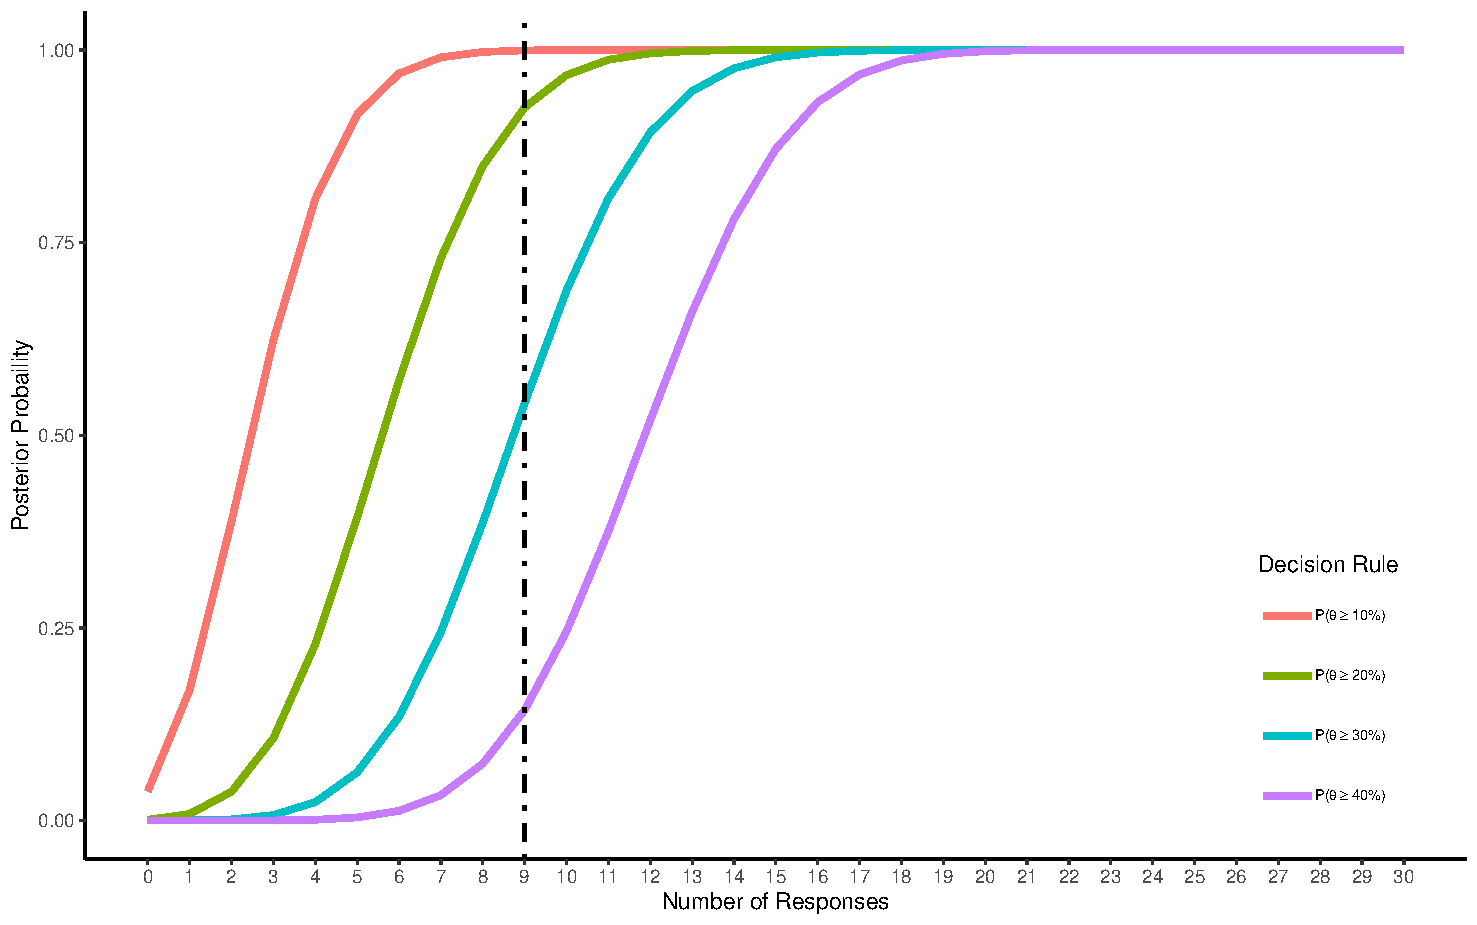
\includegraphics[width=\textwidth]{ETP-DecisionCriteria}
\end{figure}

Here we have shown how ETPs are constructed and how they change and react to modifications in our decision rules. There are several other factors which can impact an ETP such as the prior used in the Beta-Binomial conjugate analysis as well as the timing of each interim analysis and the overall sample size of the trial. Changes to the prior will have an impact on all of the calculations as it is used to generate the posterior distribution on which all of the other calculations are based upon. Adding more interim analyses would add more rows to the plot and changing the sample size of the trial alters the number of cells in each row. 

Overall ETPs can be a useful tool during the design stages of a trial as we can experiment with different decision rules and see what practical affect it has on the trial in terms of the number of responses that need to be observed for a GO decision. They can be used to facilitate discussions with non statistical experts involved in the design of the trial. Much like dose transition pathways in a dose-finding trial they can also provide some transparency as to what decisions will be made and when they would be made. 

A single ETP also provides us with the ability to see how multiple different decision rules may change the outcome for a trial. If just the acceptable probability levels for the PPoS and final analysis, $t$ and $q$, are changing in the decision rule the impact of those changes should be apparent just by comparing the PPoS and posterior probability without the need of generating a whole new plot like we have in our example.

Whilst the calculations needed to produce these plots can be quite simple actually constructing the plots is not so trivial. To overcome this issue and make ETPs easily accessible and producible, we developed a web based application to generate ETPs. All the ETPs shown so far were generated using this application. 

In the next sections we detail trials that have been designed using ETPs. These served as further motivation for development of the application to produce ETPs. We then go on to detail how the app was developed and how it works.    

%----------------------------------------------------------------------------------------
%	SECTION 4
%----------------------------------------------------------------------------------------

\section{Implementation of Efficacy Transition Pathways}

With the development of any new methodology or novel tool such as ETPs there will be some barriers that will impede its use. One of those barriers will be the difficulty of implementing the methodology. If the intention of some newly developed methodology is for it be applied in a practical setting, when presented it should be accompanied by appropriate software or code such that the target audience are able to implement it with minimal effort. Otherwise the new methodology may remain purely theoretical and would rely on others to come up with a solution for its implementation. 

To overcome this barrier for ETPs we developed a R function to produce these plots given the input of key details such as the decision criteria, sample size and cohort size. We then used this function and built a web application around it. Rather than just offering code to implement ETPs a web app makes implementation even easier as it doesn't require knowledge or experience with a specific piece of stats software such as R, STATA or SAS. 

Another barrier that limits the rate at which new methodology is implemented is a lack of awareness or familiarity with the methodology. Specifically, with clinical trials that often involve a multidisciplinary team it is unrealistic to expect clinicians or trial management to be up to date with the latest statistical innovations. Even the statisticians themselves may not be familiar with the latest methodology. As a result, newer methods may be overlooked even if it would be beneficial to implement. Even if statisticians are aware of new methodology, the struggle may then become explaining the methodology to non-statisticians and convincing them it will be beneficial to use. 

Inherently ETPs as a tool were created to help better explain the analysis that is done in these phase \RN{2} trials as well as the decisions that are made. They exist more as a tool to help promote the underlying Bayesian methodology. Therefore ETPs may be simple to implement and explain to non-statisticians. Instead the issue may come from a lack of understanding of a Beta-Binomial conjugate analysis, predictive probabilities or the background methodology behind the ETPs. 

To address this within our web application we included detailed information about ETPs as well as a breakdown of the methodology behind them. This was done through text and images in combination with custom built interactive tools that illustrates how these trials are run in a practical setting. These additional explanations and features were built in to make understanding ETPs easier, especially for those with a non stats background. These sections can also be used as a teaching tool to help educate those who are working on trials but not familiar with this methodology.  

Lucinda Billingham (LB) as the visionary behind ETPs had began implementing them in a number of different trial designs despite these barriers. Some of these trials were being designed as umbrella, basket or platform trials and involved multiple arms. Here analyses and decisions were being made in each arm independently so ETPs were employed to help design these trials. 

This leads to more issues where during the design stages of a trial multiple ETPs may need to be generated. If changes were made to specific decision criteria the ETP would need to be updated so you could communicate how those changes would affect the outcome of the trial. This is then further compounded with the complex trial designs where there may different criteria dependent on the arms in the trial.

Prior to the development of the app ETPs were being constructed by hand which was a time consuming endeavour. We will detail three trials that were designed by the Cancer Research Clinical Trials Unit (CRCTU) at the University of Birmingham and show how ETPs have previously been implemented. 

%-----------------------------------
%	SUBSECTION 1
%-----------------------------------

\subsection{MonoGerm} 

This trial was designed by Lucinda Billingham (LB) and Laura Kirton (LK). What is presented here is the design that was used as part of a grant application which has since been accepted. The trial is currently in the process of being set-up so may be subject to some design changes before it is open. 

MonoGerm \footnote{A phase II trial of carboplatin or vinblastine monotherapy induction prior to radiotherapy for patients with intracranial germinoma} is a Phase \RN{2} trial investigating, in parallel, two single-agent chemotherapies (carboplatin or vinblastine) as monotherapy prior to standard of care radiotherapy in patients with intracranial germinoma. This trial utilises a Bayesian approach for analysis and decision making. A 'flip-flop' approach is used for recruitment, this was a term coined by investigators of the trial. Essentially, recruitment will begin to the carboplatin arm then once three patients have been recruited and considered evaluable for an interim analysis recruitment flips to the vinblastine arm. This process is then repeated by switching recruitment back and forth between the two arms till recruitment is complete. 

Typically intracranial germinoma is chemosensitive but it requires radiotherapy for a cure. This mainly affects a paediatric population. For patients with localised disease standard of care involves three-drug chemotherapy consisting of ifosfamide, carboplatin and etoposide followed by subsequent radiotherapy. Treatment involving multiple chemotherapies allows for reduction in radiotherapy doses and fields. However, there is still an increased burden of treatment on patients which can cause both short and long-term harm. This can lead to patients experiencing multiple toxicities such as diabetes insipidus, myelosuppression, vomiting/diarrhoea, electrolyte disturbances, renal impairment, and elevation of liver enzymes. 

The aim of the trial is to evaluate whether a single-agent chemotherapy (carboplatin or vinblastine) is non-inferior to	the standard of care multi-drug chemotherapy for inducing complete response (CR), and is associated with reduced harm and improved quality of life. The primary outcome measure will be CR based on MRI scans at 6 and 12 weeks. 

The trial will consist of two arms, one arm for carboplatin and one for vinblastine. There will be 36 patients recruited in total, 18 per arm. Patients will be enrolled in cohorts of three to each treatment-arm by the flip-flop design. This is illustrated in Figure \ref{fig_etp:MonoGermFlipFlop}. Recruitment begins in the carboplatin arm and then once three patients have been recruited recruitment is paused and then begins in the vinblastine arm. Whilst recruitment is paused in the carboplatin arm an interim analysis will be performed for that first cohort. Here primary outcome data and key safety data will be assessed. Once recruitment to the first cohort of the vinblastine arm is complete and the interim analysis for the first cohort of carboplatin patients is done recruitment can begin for the second cohort in the carboplatin arm and the interim analysis for the first cohort of vinblastine patients can be conducted. This process is then repeated for the subsequent cohorts. This design allows for continuous enrolment and monitoring of the primary outcome. 

\begin{figure}[h!]
	\centering
	\caption{Flip-flop recruitment design in the MonoGerm trial.}
	\label{fig_etp:MonoGermFlipFlop}
	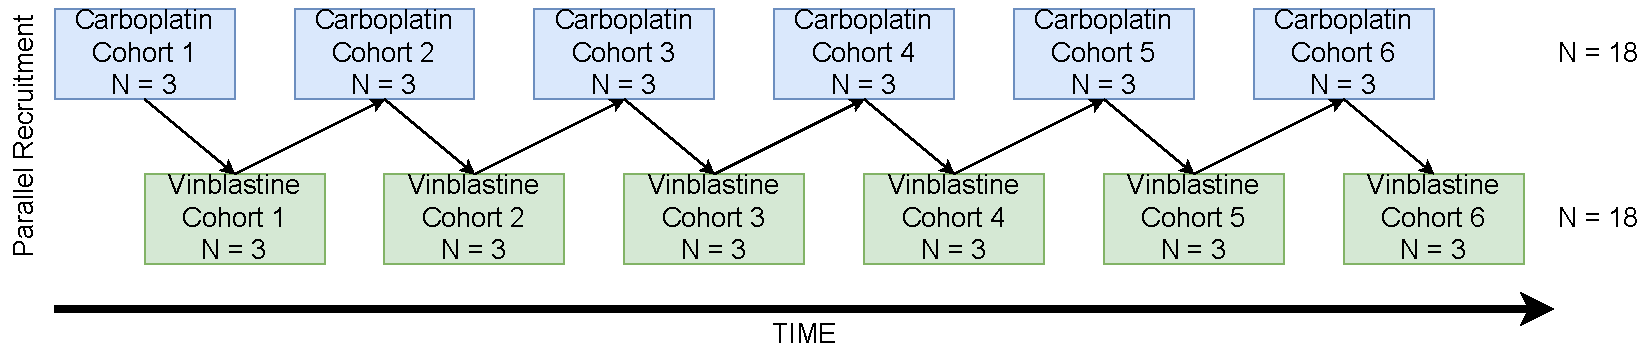
\includegraphics[width=\textwidth]{ETP-MonoGermFlipFlop}
\end{figure}

A Bayesian approach is implemented to assess the true CR rates. Specifically, the experimental monotherapies will need to demonstrate non-inferiority to the standard of care by a clinically acceptable margin. Based on previous data it was determined that the minimum CR rate with standard of care is 30\%. This value was taken as the non-inferiority margin. So, if the treatments have a CR rate $\geq30$\% they will be considered non-inferior. 

CR rates for each treatment arm will be established from the posterior probability distribution generated using a beta-binomial conjugate analysis. A minimally informative Beta(1,1) prior will be used in combination with the data observed during the trial to produce the posterior. In terms of decision making the following rule for the final analysis was specified: 

\begin{equation}
	P(CR \geq 30) \geq 0.8
\end{equation}

That is to say that if there is a high probability ($\geq 0.8$) that the true CR rate is $\geq30$\% there will be a GO decision. Which in the context of this trial means the treatment arm would be deemed non-inferior. The minimum number of observed CRs out of the 18 patients needed to warrant a GO decision is seven. If seven responses are observed the median Bayesian estimate of the CR rate would be 40\% with a 0.82 probability that the true CR rate is $\geq30$\%. 

Stopping rules have also been implemented. At each interim analysis the predicted probability of success (PPoS) will be calculated. This is the probability that a GO decision would be made at the final analysis based on current data that has been accrued. Here the stopping rule is such that if the PPoS is less than 0.01 we would recommend stopping recruitment to that arm. 

It is important to note that whilst the trial has two arms it is not designed with the intention of making comparisons between the two treatments. Rather the trial aims to find if there is enough evidence that one of these treatments provides a sufficient response rate to warrant a GO decision.  

LK produced ETPs throughout the design of this trial. Figure \ref{fig_etp:MonoGermETP} shows the ETP for the design specified here. The ETPs produced here helped determine what data we wanted to present as well as how we structure the data in each of the cells. Here each cell shows the number of responses, the PPoS or the posterior probability that the response rate is $\geq30$\%, the Bayesian estimate of CR rate and a lower one-sided 80\% credible interval.

Calculations for these plots were conducted in STATA and the ETP was produced in Microsoft PowerPoint. One benefit of this approach is that the ETP can be easily customised and labelled. However, this meant that any changes in the design that affected the decision-making resulted in the ETP having to be updated manually. As a tool the ETP is effective at illustrating a final design but without the ability to easily generate them during the design of a trial they somewhat lose their purpose. This served as further motivation to produce some code or a tool that would allow for ETPs to be automatically created. 

\begin{sidewaysfigure}[h!]
	\centering
	\caption{ETP for the MonoGerm trial.}
	\label{fig_etp:MonoGermETP}
	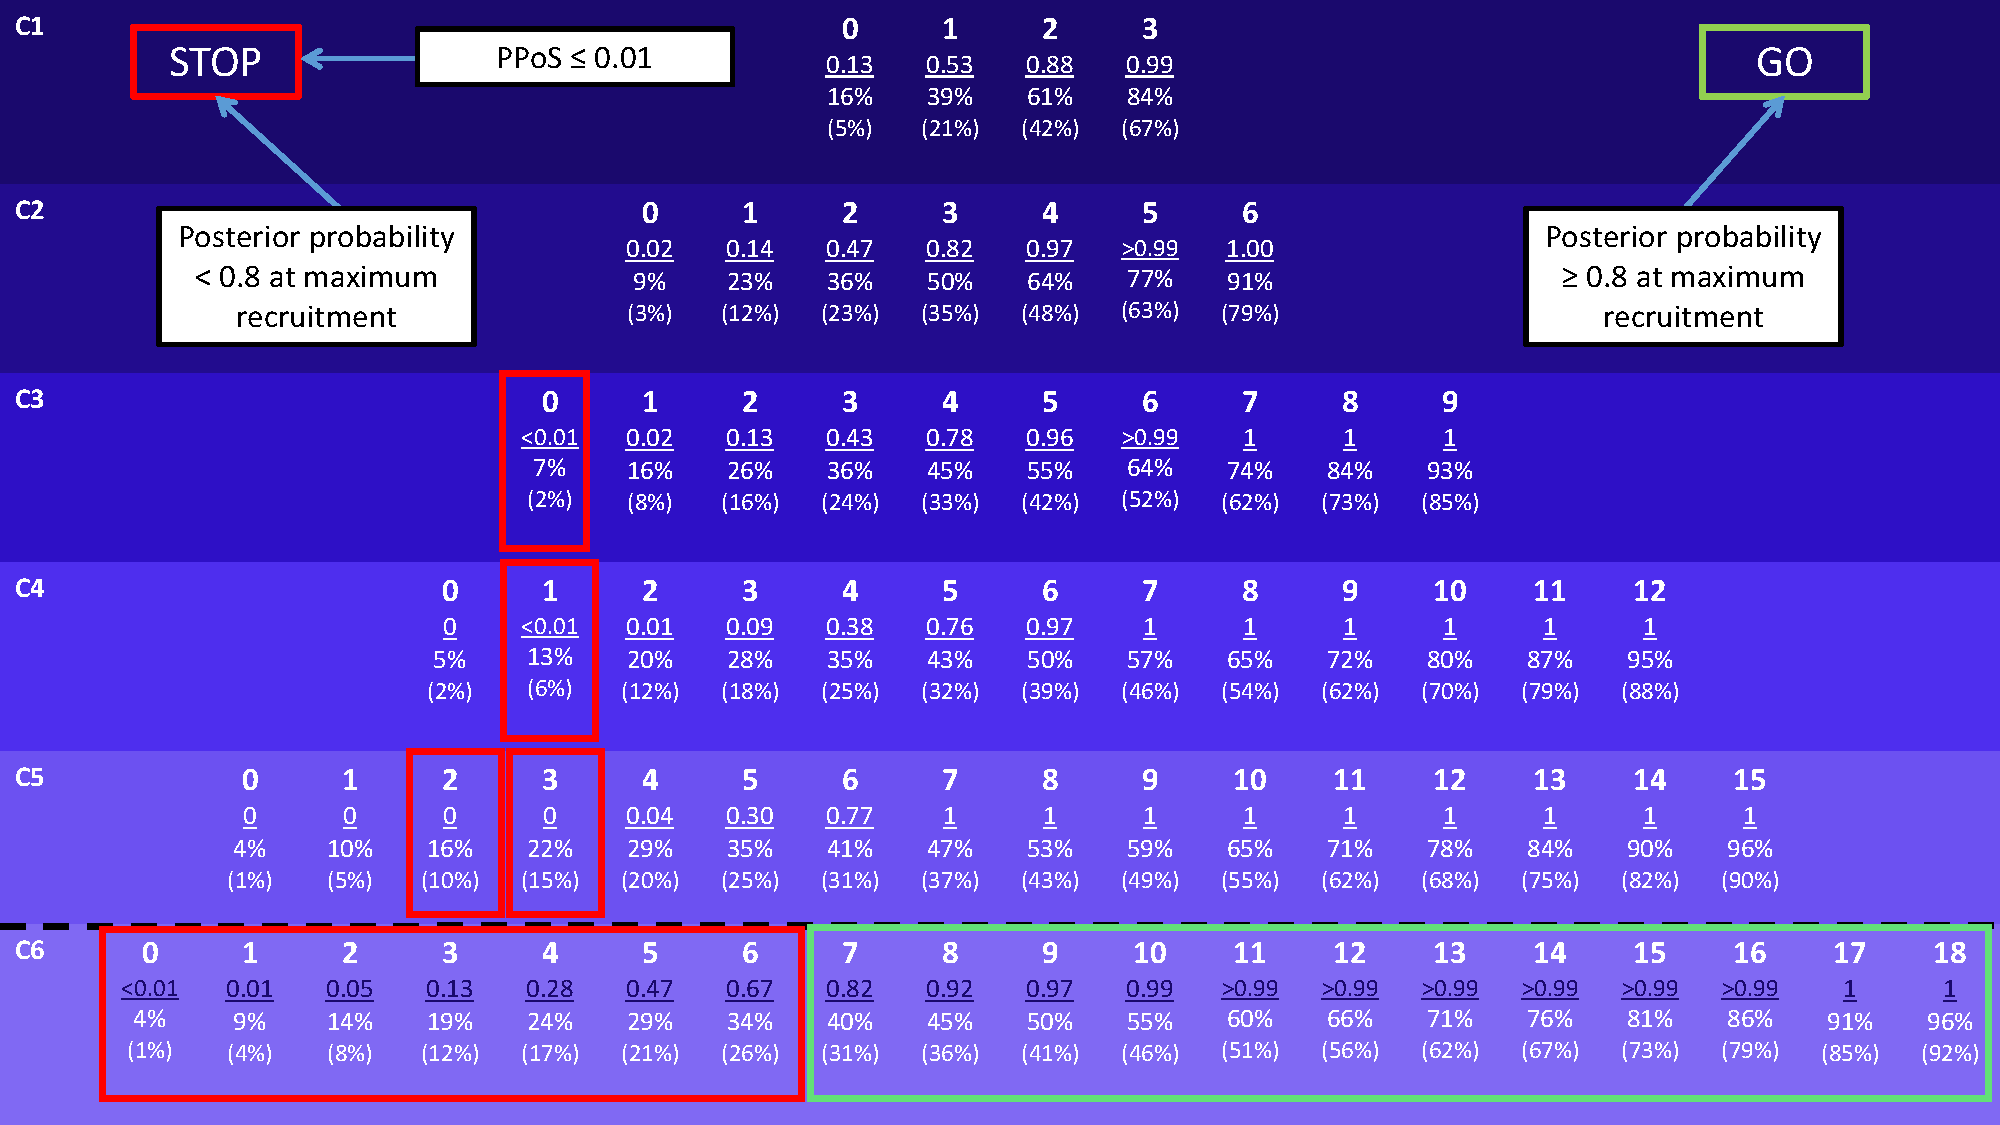
\includegraphics[width=23cm, height=15cm]{ETP-MonoGermETP}
\end{sidewaysfigure} 

\clearpage

%-----------------------------------
%	SUBSECTION 2
%-----------------------------------

\subsection{Glo-BNHL}

This trial was designed by Lucinda Billingham (LB) with the assistance of Shanna Maycock (SM). During initial stages of the design Grace Holt (GH) also assisted with the implementation of ETPs. This trial is currently still in set-up so specific details of the trial may be subject to change.   

The Glo-BNHL \footnote{A Global Study of Novel Agents in Paediatric and Adolescent Relapsed and Refractory B-cell Non-Hodgkin Lymphoma} study is a platform trial that aims to investigate the safety and effectiveness of novel treatments in children, adolescents and young adults with relapsed and/or refractory B-cell non-Hodgkin Lymphoma (r/r BNHL). This trial is an international collaboration and hopes to generate substantial evidence that could change practice in this rare cancer population. 

Inclusion of novel agents into the platform will be determined by an international Trial Steering Committee (TSC). Currently the platform consists of three separate treatment arms, each focusing on a different novel agent in a distinct group of patients. Each treatment arm will be treated independently which allows for them to be analysed separately. There may also be separate eligibility criteria for each arm. Patients will be enrolled into any arm where they are eligible. The three arms that will be available at the start of the trial are as follows: 

\begin{itemize}
	\item Treatment Arm \RN{1}: Bispecific Antibody (BsAb)
	\item Treatment Arm \RN{2}: Antibody-Drug Conjugate (ADC) with standard \\ chemotherapy
	\item Treatment Arm \RN{3}: Chimeric Antigen Receptor (CAR) T-cells
\end{itemize}

This trial utilises an adaptive Bayesian design, which enables GO/No GO decisions specific to the distinct populations in each treatment arm. The Bayesian approach has many benefits here as it facilitates decision making with small sample sizes. Decisions will be made based on the estimate of the probability that a novel agent is clinically effective. The specific criteria will vary between each treatment arm. This design and approach also allows for continuous evaluation of each novel agent. Treatment arms may be removed if the treatment is shown to be ineffective based on the trial data. Additionally, treatment arms may also be added or amended in the future if recommended by the TSC. 

Treatment arm \RN{1} aims to estimate the clinical efficacy of BsAb treatment in patients with r/r BNHL in first (only one prior line of therapy) or subsequent relapse (more than one prior line of therapy). Due to this treatment arm \RN{1} is split into two groups, \RN{1}a and \RN{1}b for patients with one relapse or more than one relapse respectively. These two subsequent arms will be recruited into and analysed separately. In terms of treatment these patients will receive odronextamab given as an intravenous infusion weekly for 12 weeks, then every two weeks until nine months, and every four weeks thereafter until progression or for a maximum of two years. The outcome measure for patients in treatment arms \RN{1}a and \RN{1}b is the occurrence of an objective response (OR) i.e. complete response (CR) or partial response (PR) after 12 weeks of treatment assessed by Independent Central Review. However, for interim analyses local response assessments will be used. 

Treatment arm \RN{2} aims to estimate the clinical efficacy of ADC treatment with modified R-ICE (rituximab, ifosphamide, carboplatin, etoposide and dexamethasone) chemotherapy in patients with r/r B-NHL in first or subsequent relapse. Patients will receive loncastuximab tesirine given as a 30 minute intravenous infusion with each cycle of modified R-ICE for a maximum of three cycles. Here the outcome measure is occurrence of CR within a maximum of three cycles of treatment. 

Treatment arm \RN{3} aims to estimate the efficacy of CAR T-cell therapy in r/r B-NHL patients who have CAR T-cell product available. The specific treatments patients will receive is yet to be defined. The outcome measure is the occurrence of OR following CAR T-cell infusion. 

Each treatment arm and subsequent treatment arm (i.e. \RN{1}a and \RN{1}b) will aim to recruit 15 evaluable patients during the initial stage. Once this recruitment is complete a transition analysis is performed leading to three possible outcomes. If the analysis results in a No GO decision recruitment to that treatment arm will stop. If the analysis result is a GO decision there are two options either there is sufficient evidence to change practice so the trial will stop recruiting or this will trigger an expansion stage in which a further 15 patients will be recruited. Following the expansion stage a confirmatory analysis will be conducted on all 30 evaluable patients. 

Interim analyses will be conducted after every three patients during the initial stage and after every five patients during the expansion stage. There will also be the option to stop recruitment to a treatment arm based on the data observed in the interim analysis. Figure \ref{fig_etp:Glo-BNHLflowchart} shows a flowchart of the decision making process for each arm in the trial. 

\begin{figure}[h!]
	\centering
	\caption{Flowchart of the decision making process in Glo-BNHL.}
	\label{fig_etp:Glo-BNHLflowchart}
	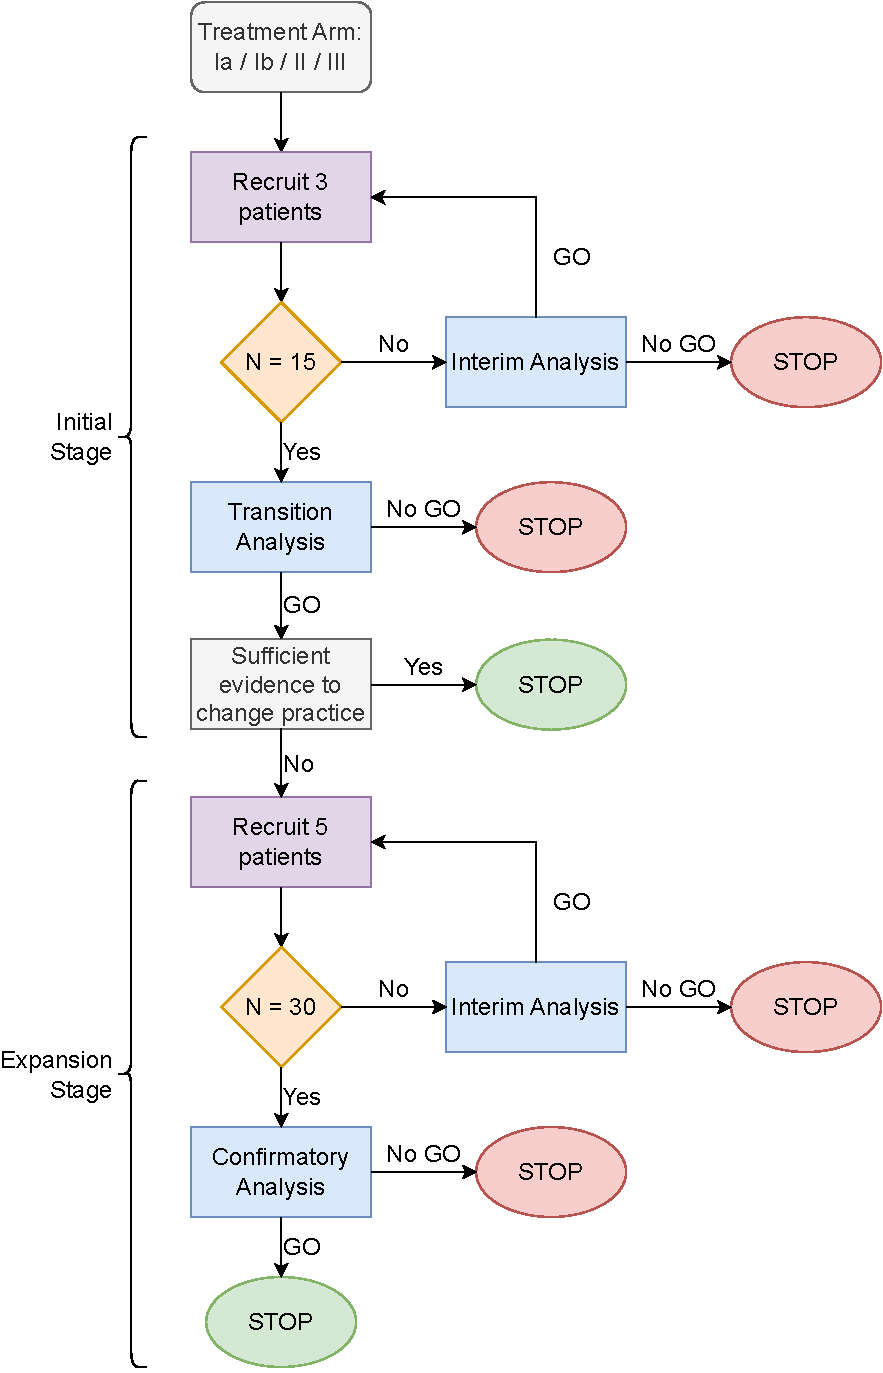
\includegraphics[width=0.9\textwidth]{ETP-GloBNHL-flowchart}
\end{figure}

A beta-binomial conjugate analysis will be conducted for each treatment arm. Observed trial data will be combined with a minimally informative Beta(1,1) prior to produce a posterior probability distribution for the treatment effect $\theta$, which represents either the OR/CR rate dependent on treatment arm. The posterior probability distribution is then used to inform decision making. GO/No Go decision criteria are specified separately for each treatment arm. 

For treatment arm \RN{1}a the decision criteria at the transition analysis is P($\theta$ > 40\%) $\geq$ 0.8. So, if the true OR rate was greater than 40\% with a probability of at least 0.8 based on the data collected in the trial there would be a GO decision. This corresponds to observing at least eight responses out of 15. For the confirmatory analysis a GO decision is made if P($\theta$ > 40\%) $\geq$ 0.95. At the final analysis we would need the probability that the true OR rate was greater than 40\% to be at least 0.95. Here a GO decision would only be made if 17 out of 30 patients had an OR. Table \ref{tab_etp:GloBNHL_decision_criteria} details the criteria for each treatment arm which can be interpreted in a similar manner. 

\begin{table}[h!]
	\centering
	\caption{Summary of decision criteria for Glo-BNHL.}
	\label{tab_etp:GloBNHL_decision_criteria}
	\resizebox{\textwidth}{!}{%
		\begin{tabular}{ccccc}
			\hline
			\multicolumn{1}{l}{\textbf{}} & \multicolumn{2}{c}{\textbf{Transition Analysis}}               & \multicolumn{2}{c}{\textbf{Confirmatory Analysis}}             \\ \cline{2-5} 
			\textbf{Treatment Arm}        & \textbf{Decision Criteria} & \textbf{Min No. Responses for GO} & \textbf{Decision Criteria} & \textbf{Min No. Responses for GO} \\ \hline
			Ia  & P($\theta$ \textgreater 40\%) $\geq$ 0.8 & 8/15 & P($\theta$ \textgreater 40\%) $\geq$ 0.95 & 17/30 \\
			Ib  & P($\theta$ \textgreater 10\%) $\geq$ 0.8 & 3/15 & P($\theta$ \textgreater 10\%) $\geq$ 0.95 & 6/30  \\
			II  & P($\theta$ \textgreater 20\%) $\geq$ 0.8 & 5/15 & P($\theta$ \textgreater 20\%) $\geq$ 0.95 & 10/30 \\
			III & P($\theta$ \textgreater 10\%) $\geq$ 0.8 & 3/15 & P($\theta$ \textgreater 10\%) $\geq$ 0.95 & 6/30  \\ \hline
		\end{tabular}%
	}
\end{table}

For the interim analyses there are separate stopping rules. These are the same across the treatment arms but differ in the initial stage compared to the expansion stage. During the initial stage, the predicted probability of success at the transition analysis (PPoSt) is calculated and decisions are made based on the following criteria: 

\begin{enumerate}
	\item PPoSt < 0.01 - recommend stopping for futility
	\item 0.01 $\leq$ PPoSt < 0.05 - consider stopping for futility
	\item 0.05 $\leq$ PPoSt < 0.15 - consider whether sufficient benefit in continuing 
	\item PPoSt $\geq$ 0.15 - recommend continuing 
\end{enumerate}

So, if the probability of success at the transition analysis is less than 1\% the recommendation would be to stop recruitment to the treatment arm and if it was greater than or equal to 15\% the recommendation would be to continue recruitment. If PPoSt is between 1-5\% or 5-15\% stopping should be also be considered for either futility or if there sufficient benefit in continuing respectively.  

At the expansion stage, the predicted probability of success at the confirmatory analysis is used (PPoSc). If this is below 10\% (PPoSc < 0.1) the recommendation would be to stop recruitment to that treatment arm due to futility. It should be noted that these decision rules are only recommendations and the independent data monitoring committee (DMC) will make decisions based on not only primary outcomes but secondary outcomes, recruitment and safety data. 

For this trial ETPs were produced separately for each treatment arm and for each stage. This resulted in eight ETPs, one for the initial stage showing the outcome of the transition analysis and one for the expansion stage showing the outcome of the confirmatory analysis for each treatment arm (\RN{1}a, \RN{1}b, \RN{2}, \RN{3}). ETPs were utilised throughout the design of the trial with initial versions originally created by GH using STATA and Microsoft PowerPoint. These were then further developed by SM who performed calculations in R but still utilised PowerPoint to create the ETPs. Figure \ref{fig_etp:GloBNHL-ETP-TA1aInitial} and \ref{fig_etp:GloBNHL-ETP-TA1aExtenstion} shows the ETPs for the initial and expansion stage of treatment arm \RN{1}a respectively. These ETPs created by SM helped us determine how our function and app visually presented ETPs and we utilised a similar colour scheme. 

Similar to MonoGerm the process of creating these ETPs in PowerPoint can be time consuming. This is even more of an issue in the Glo-BNHL study due to the multiple treatment arms and stages. Additionally, this trial highlighted another issue when you have multiple statisticians working on a trial who use different software packages. In this case it would mean work would have to be recreated in R and STATA to conduct the calculations required for ETPs. This served as further motivation for the development of an application which requires no specific stats software knowledge. As statisticians would easily be able to recreate ETPs. SM went on to further extend the function we developed to automatically generate ETPs specific to Glo-BNHL. 

\begin{sidewaysfigure}[h!]
	\centering
	\caption{ETP for the initial stage of treatment arm \RN{1}a in Glo-BNHL.}
	\label{fig_etp:GloBNHL-ETP-TA1aInitial}
	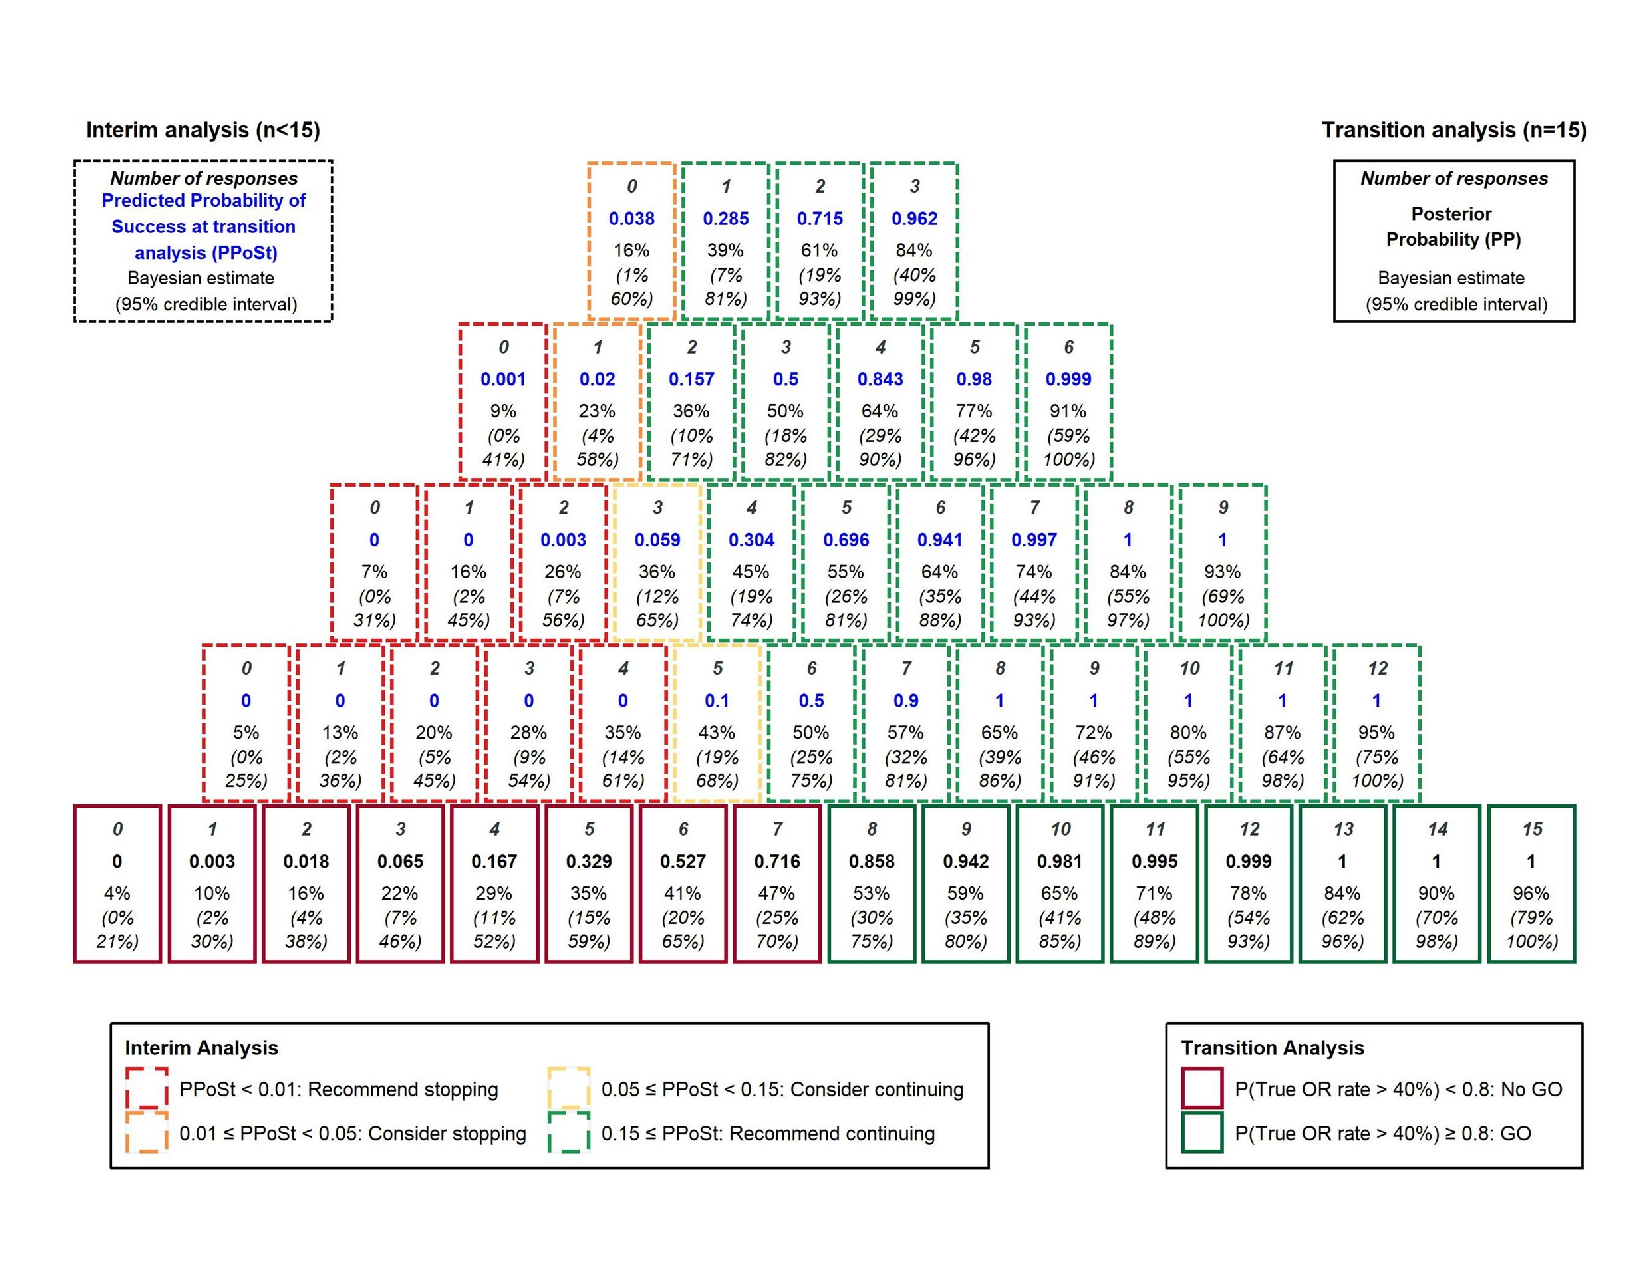
\includegraphics[width=23cm, height=15cm]{ETP-GloBNHL-ETP-TA1aInitial}
\end{sidewaysfigure} 

\begin{sidewaysfigure}[h!]
	\centering
	\caption{ETP for the expansion stage of treatment arm \RN{1}a in Glo-BNHL.}
	\label{fig_etp:GloBNHL-ETP-TA1aExtenstion}
	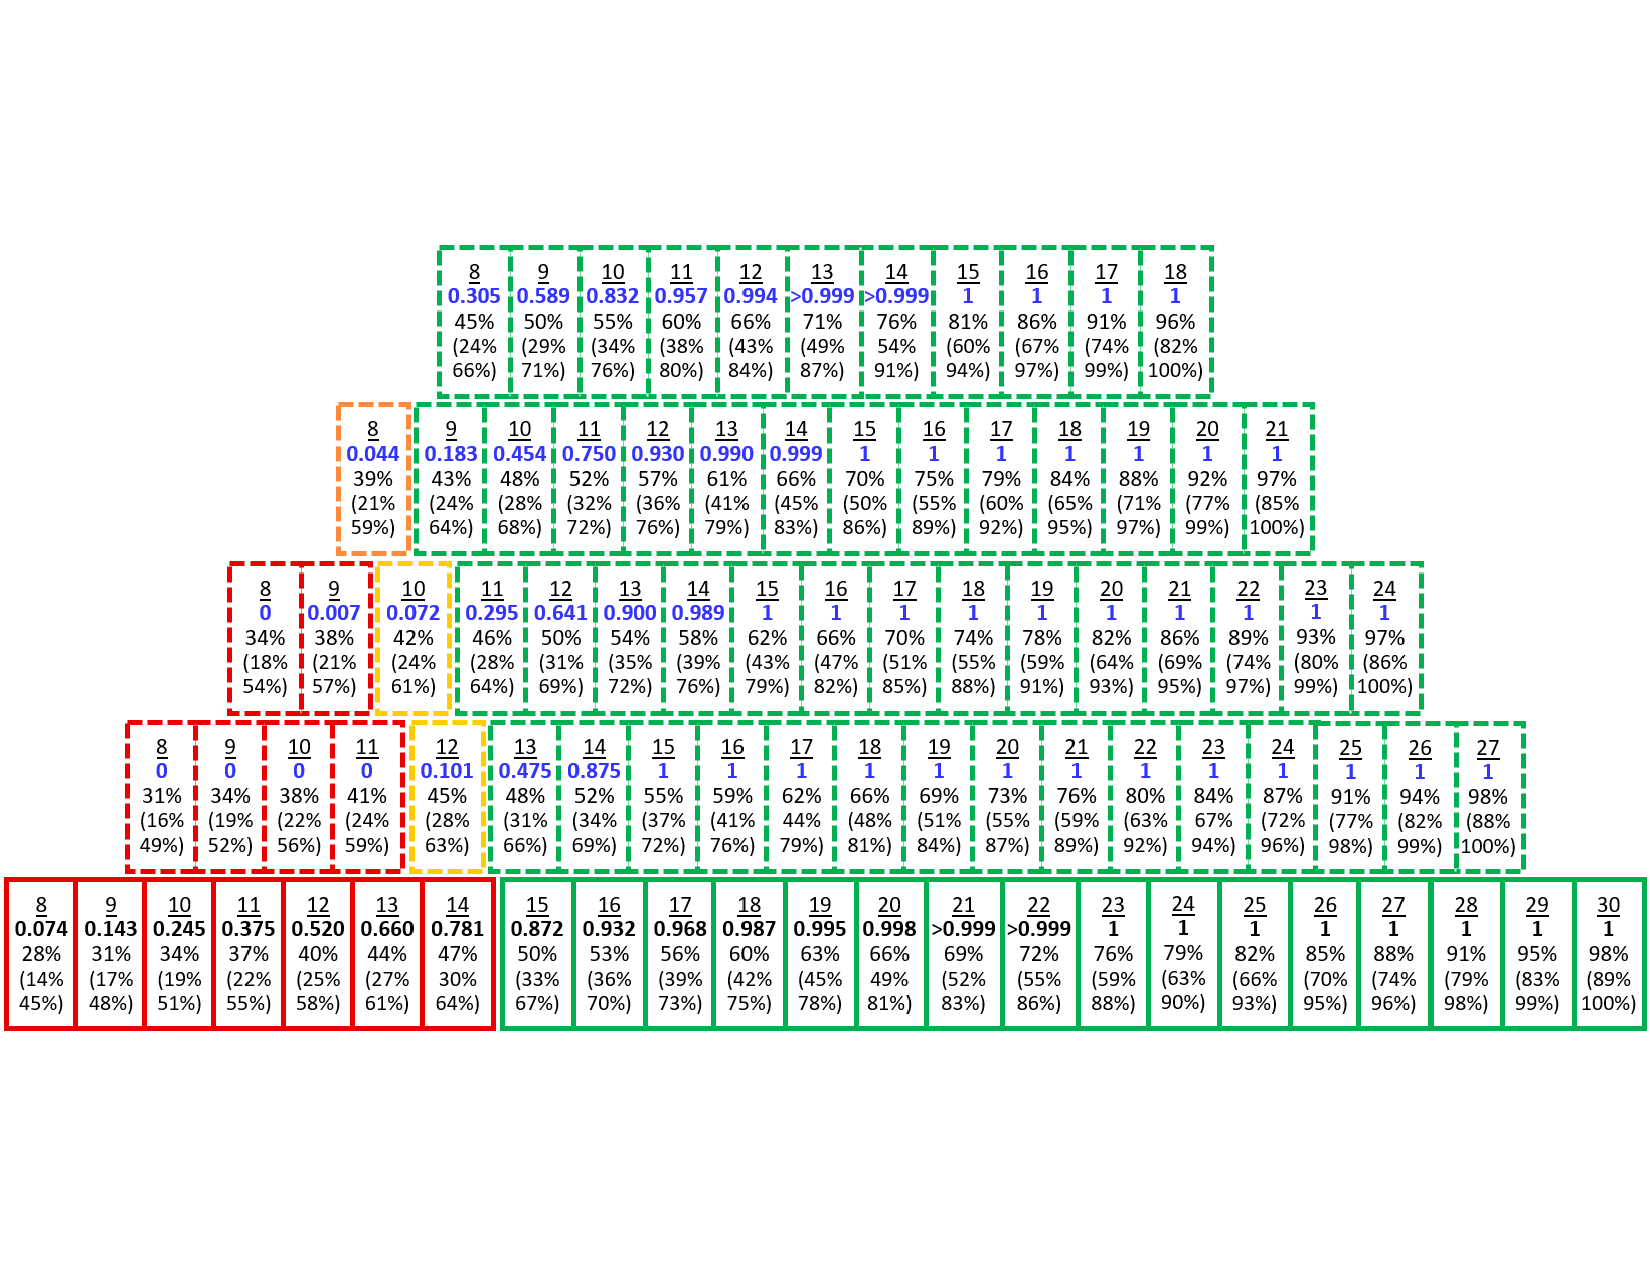
\includegraphics[width=23cm, height=15cm]{ETP-GloBNHL-ETP-TA1aExtension}
\end{sidewaysfigure} 

\clearpage

%-----------------------------------
%	SUBSECTION 3
%-----------------------------------

\subsection{DETERMINE}

DETERMINE \footnote{Determining Extended Therapeutic indications for Existing drugs in Rare Molecularly-defined Indications using a National Evaluation platform trial} is a trial that was also designed by Lucinda Billingham (LB). It is an umbrella-basket platform trial with multiple treatment arms running in parallel. The trial aims to evaluate the efficacy of targeted therapies in rare cancers with actionable genomic alterations, including common cancers with rare actionable alterations. This trial is currently open to recruitment and may be expanded in the future as more drugs are bought onto the platform.  

DETERMINE will recruit patients of all ages including, paediatric, TYA (teenage and young adult) and adults, who have rare tumours that contain an actionable genetic alteration that can be targeted therapeutically. The genetic alteration must have been identified previously from a tissue biopsy or ctDNA (circulating tumour DNA). Patients will then be stratified into molecular groups based on their tumour profile and allocated to the most suitable treatment arm by the Molecular Tumour Board (MTB). The umbrella part of the design consists of multiple non-randomised treatment arms, each evaluation a licensed targeted anti-cancer drug or drug combination in a specific molecularly-defined group of patients. Each molecularly-defined group allocated to a specific treatment arm will contain multiple baskets of different tumour types, age groups and molecular subtypes. This is visualised in Figure \ref{fig_etp:DETERMINEDesign}. 

\begin{figure}[h!]
	\centering
	\caption{Umbrella-basket platform trial design in DETERMINE.}
	\label{fig_etp:DETERMINEDesign}
	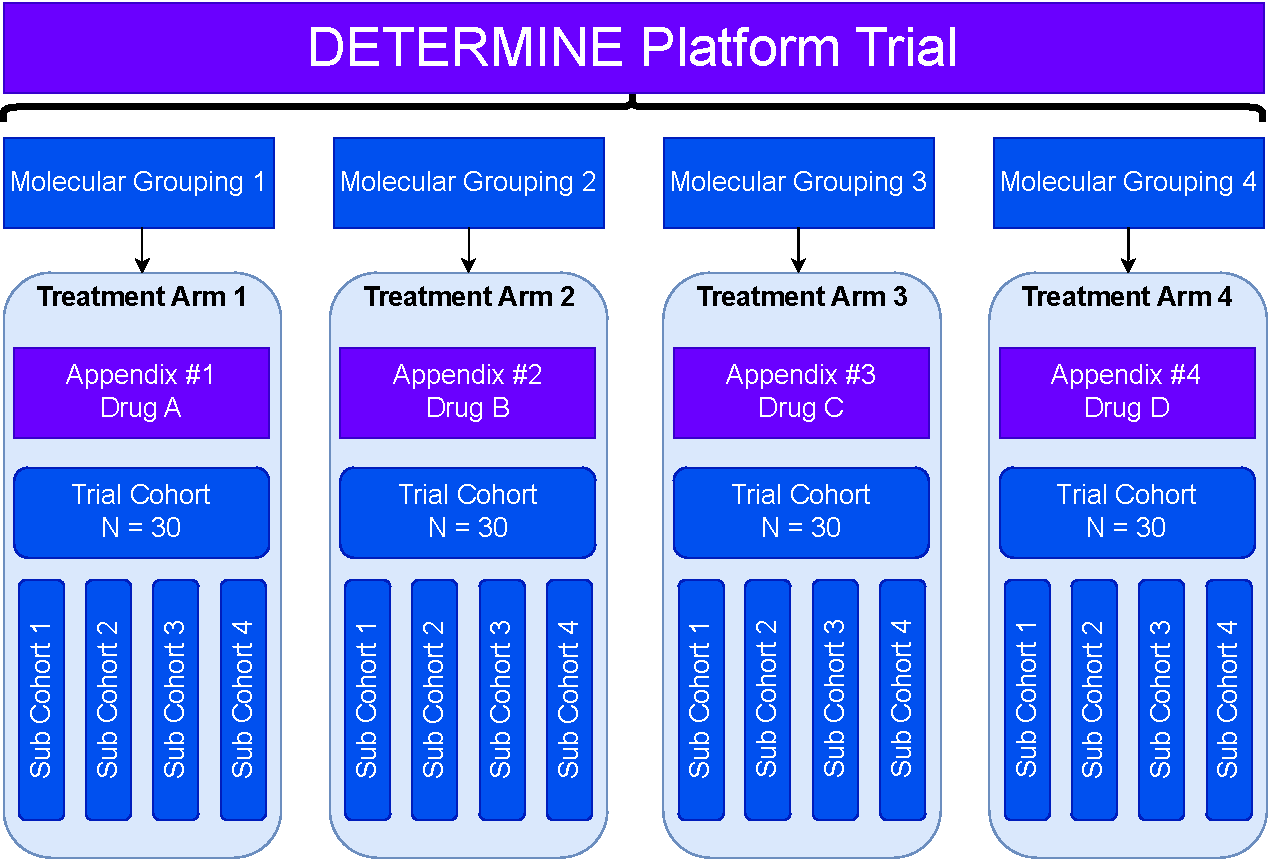
\includegraphics[width=\textwidth]{ETP-DETERMINEDesign}
\end{figure}

A main trial cohort of 30 evaluable patients will be recruited into each treatment arm. This will include patients with different tumour types, ages and molecular subtypes. If specific subgroups within this main cohort are experiencing significant benefit from treatment sub-cohorts will be formed to investigate treatment effectiveness in these subgroups. It is possible for each treatment arm to have multiple sub-cohorts and they can recruit in parallel to the main cohort. Each sub-cohort will be subject to the same statistical analysis and will also aim to recruit 30 patients. Currently there are five treatment arms, details of these are provided in Table \ref{tab_etp:DETERMINE_trtarms}. 

\begin{table}[h!]
	\fontsize{10pt}{10pt}\selectfont
	\centering
	\caption{Current treatment arms in DETERMINE}
	\label{tab_etp:DETERMINE_trtarms}
	\resizebox{\textwidth}{!}{%
		\begin{tabular}{p{0.1\textwidth} | p{0.2\textwidth} | p{0.5\textwidth} | p{0.2\textwidth}}
			Treatment Arm  & IMP(s) & Molecular Grouping & Route and Formulation \\ \hline
			1 &  Alectinib & ALK gene fusion positive solid tumours & Oral capsules \\ \hline
			2 & Atezolizumab & Solid tumours with high tumour mutational burden (TMB) or microsatellite instability-high (MSI-high) or proven constitutional mismatch repair deficiency (CMMRD) disposition & Intravenous (IV) infusion  \\ \hline
			3 & Entrectinib & NTRK or ROS1 gene fusion positive solid tumours & Oral capsules; Dosing depends on body surface area (BSA) \\ \hline
			4 & Trastuzumab in combination with pertuzumab & Solid tumours with HER2 amplification or mutations & IV infusion \\ \hline 
			5 & Vemurafenib in combination with cobimetinib & Solid tumours with BRAF V600 mutations & Oral; 960 mg tablets \\ \hline
		\end{tabular}
	}
\end{table}

Co-primary outcomes of objective response (OR) and durable clinical benefit (DCB) will be used to assess efficacy of the treatment in each of the cohorts in each molecular grouping. These are both classified as binary variables. OR is defined dependent on specific disease criteria. DCB is defined as the absence of disease progression for at least 24 weeks from the start of trial treatment, this will also be measured based on disease specific criteria. Patients will receive treatment based on the license schedule for the drug in their treatment arm. Patients continue treatment until either they reach progressive disease (PD), unacceptable adverse events or withdraw from the trial. 

All outcomes in each treatment arm, cohort and sub cohort will be analysed using a Beta-Binomial conjugate analysis. Posterior probability distributions for OR and DCB will be generated using minimally informative priors, Beta(0.1,0.9) and data that is collected on the trial. However decision making will be done using the BOP-2 design \cite{zhouBOP2BayesianOptimal2017}. This design makes GO or No GO decisions by assessing posterior probabilities for a set of outcomes, which are optimised to either maximise power or minimise the number of patients. The design also allows for the control of type I and type II error rates. In DETERMINE, for each co-primary outcome, a rate of 10\% or less would represent a treatment effect that is not clinically relevant and a rate of 30\% would represent a clinically meaningful treatment effect. These can be thought of as a null and alternative hypothesis. 

Interim analyses will be conducted throughout the trial, however formal decision making will first be conducted after 10 evaluable patients have been recruited and then every 5 patients from that time-point in each cohort/sub-cohort. If probability that both the true OR and DCB rates are lower than the critical threshold of 10\% the trial would recommend stopping. The design is optimised to minimise the type II error i.e. to minimise the probability of not rejecting the null hypothesis when treatment is effective. This is done whilst controlling the type I error rate at 0.1. Under the BOP-2 design this provides the following stopping boundaries of 0/10, $\leq$1/15, $\leq$2/20, $\leq$3/25 at each of the planned analyses at 10, 15, 20 and 25 patients. For the final analysis at 30 patients there would be a GO decision if $\geq$6/30 patients had either a OR or DCB.   

The ETPs we have shown so far all have been based on a Beta-Binomial conjugate analysis with decisions made using PPoS and the posterior distribution. However, they can also be utilised here. LB created the ETP shown in Figure \ref{fig_etp:DETERMINE-ETP}. Here we can see each cell still pertains to a specific number of responses out of a certain number of patients. Bayesian estimates, credible intervals and posterior probabilities of the treatment effect being greater than our null and alternative hypothesis. The cells have then been colour coded based on the decision criteria elicited from the BOP-2 design. This trial also shows that ETPs are a flexible tool that can also be applied to trials not explicitly using a Beta-Binomial conjugate analysis for decision making. 

\begin{sidewaysfigure}[h!]
	\centering
	\caption{ETP for the DETERMINE trial.}
	\label{fig_etp:DETERMINE-ETP}
	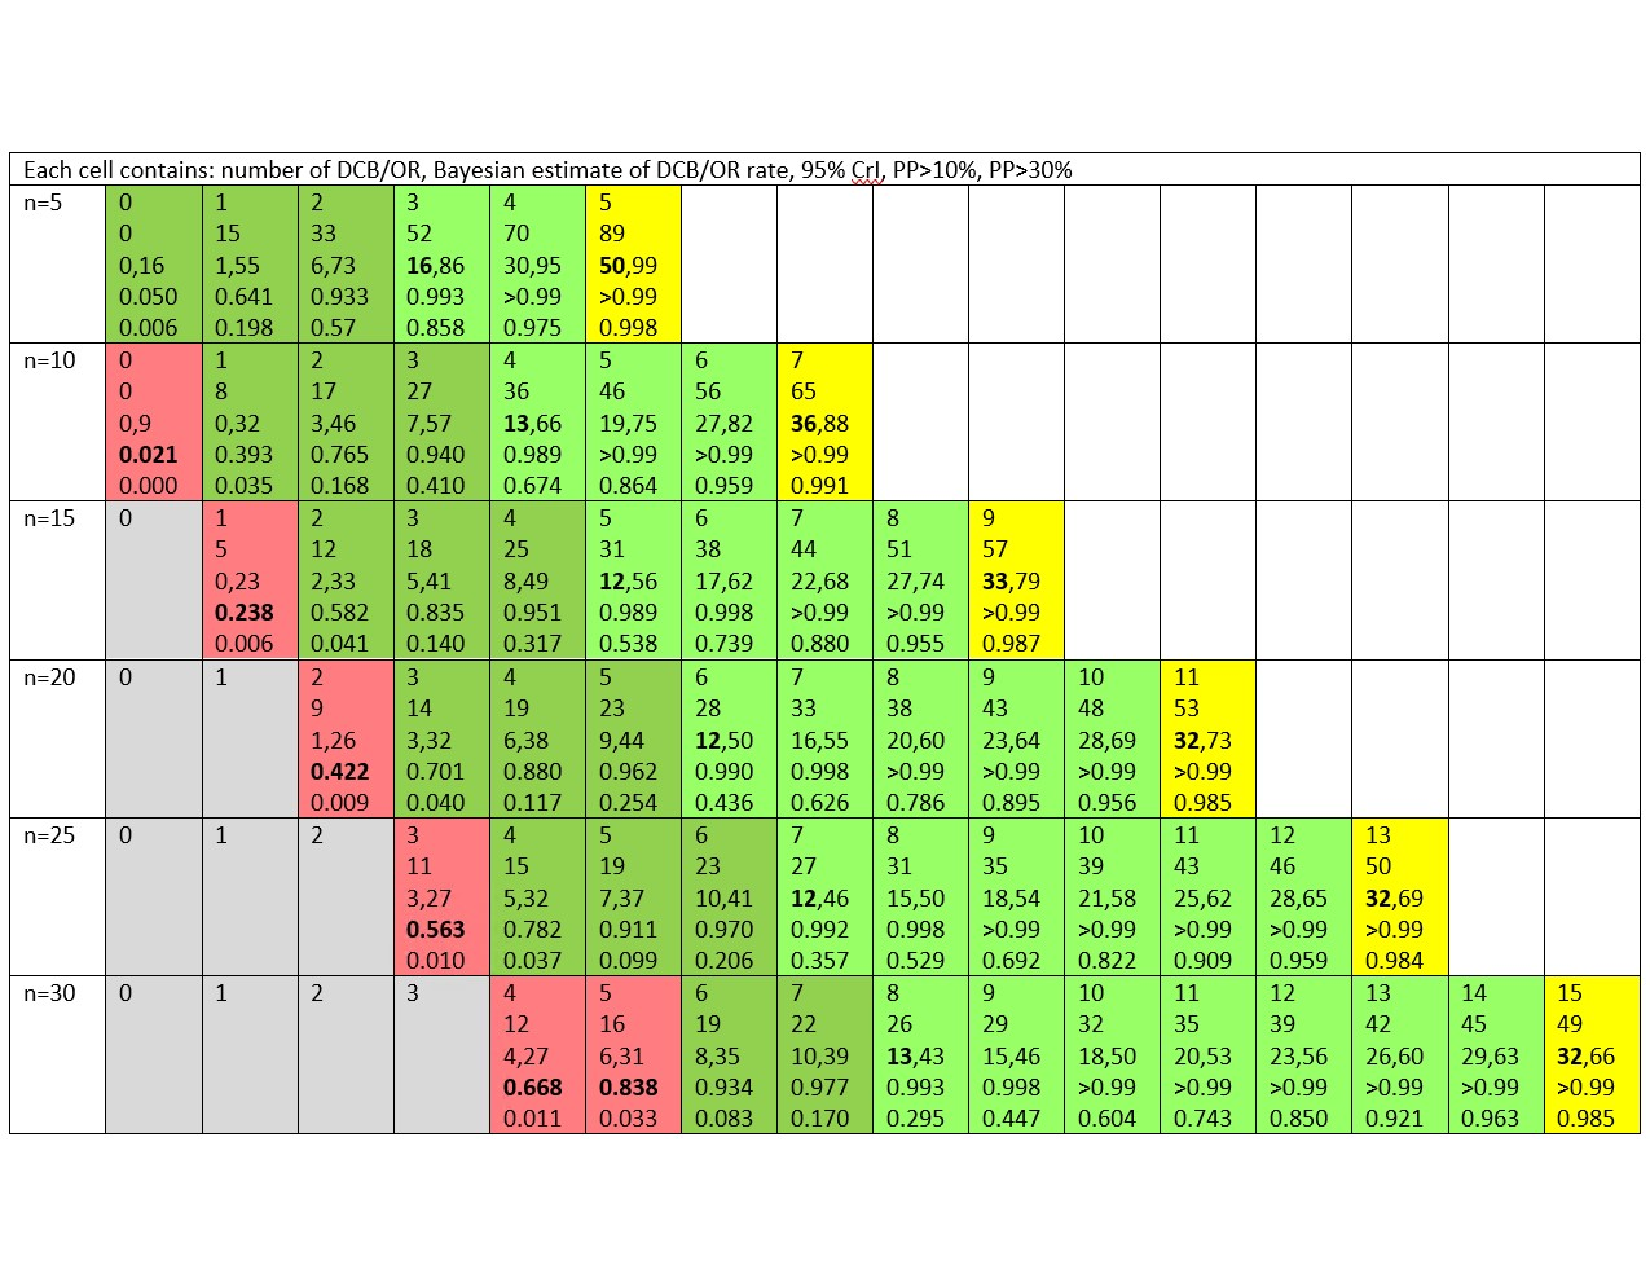
\includegraphics[width=23cm, height=15cm]{ETP-DETERMINE-ETP}
\end{sidewaysfigure} 

\clearpage

%-----------------------------------
%	SECTION 4
%-----------------------------------

\section{Development of a Web Application for Efficacy Transition Pathways}

Initially a R function was produced that was able to create ETPs. Then using R Shiny an application was built which utilised this function to produce ETPs. Whilst the R function makes implementing ETPs a lot easier, the R Shiny app offers an even better solution. Firstly, it doesn't require any previous knowledge of a specific statistical package so any statistician should be able to use the application with ease. This also applies for non-statisticians and an application would make ETPs more accessible. 

R Shiny also has the ability to make graphs interactive. Whilst ETPs produce a lot of information they are static in nature. As such a change in parameters or design characteristics means that a separate ETP would need to be produced. With R shiny a interface allows for these changes to be easily made and the plots automatically be updated. Additionally, elements of interactivity can also be included in an application. In the application by clicking on a specific cell of the ETP we produce additional plots which give the user more details than they would otherwise get with just a single ETP. The ETPs presented in Sections \ref{etp:conETPs} and \ref{etp:updatingETPs} were all produced in a few clicks using this app. 

In our app we have a specific page which is labelled "plot builder" that will generate ETPs. This page is split into two sections. The section on the left can be considered as the input and the section on the right is the output. There are three tabs in the input section and each one deals with a separate set of input parameters. The prior parameters tab allows the user to specify priors that are being used in the beta-binomial conjugate analysis and also produces a plot of the corresponding beta distribution. The app can be accessed at the following link - \href{ https://amit-patel.shinyapps.io/beta-binomialapp/}{https://amit-patel.shinyapps.io/beta-binomialapp/}. A video demonstrating the key features of the app is also available on YouTube through this link - \href{ https://www.youtube.com/watch?v=vfVzwBDp9-E}{https://www.youtube.com/watch?v=vfVzwBDp9-E}.

The design parameters tab allows the user to specify the details of their trial and all the relevant information required to produce an ETP. This includes the number of cohorts and the size of each cohort, this assumes that an interim analysis will be performed once each cohort has been recruited. Details also need to be inputted regarding the decision criteria at both the interim analysis and final analysis stage. As these design parameters are inputted the output in the right hand side section named 'Decision Rules' also updates. Here the decision criteria based on the inputs are presented to the user in a mathematical format. There is also text to explain what each of the rules mean so the users can ensure they have inputted the correct details. The interpretation will also be useful for non statisticians and provide some understanding of the decision criteria and what it means.  

The final input tab is for parameters corresponding to the visualisation of the plot. These correspond to arguments within the R function which allow the user to adjust how the ETPs look. There is the ability to change the alignment of the ETP such that the cells are either centred or left aligned. There is also an option to change the size of the text in the ETP. As ETPs can become more and more complicated depending on the design of the trial the text may become over crowded so would need to be adjusted, which is what this option allows for. There is also the option to turn the legend on and off. 

In the output section the tab labelled "Efficacy Transition Pathway" contains the ETP which is generated based on all the inputs from the input section (prior, design and plot parameters). The user can clearly see what the ETP for their given design would look like. From here the user also has the ability to download the ETP in multiple formats. Any changes made to the input parameters will result in the ETP being updated. This allows for the user to easily and quickly make tweaks to the trial design and see how the decisions made would change. They can also easily save/download all versions of the ETPs they make to compare across the different designs. 

There is also an added layer of interactivity that was incorporated into the app. By clicking on an individual cell in the ETP additional information and plots will be generated. Once a cell has been clicked on a line of text will appear below the ETP which provides specific details about what each of the numbers in the cell represent. Additionally, there will also be a plot of the individual cell with added text to explain what each number in the cell represents. This will allow users to investigate and further explore individual cells. This is specifically useful in scenarios where the ETP may be large and contain many cells and some may not be clear on the ETP. Additionally, a posterior distribution plot is also generated when a user clicks on a specific cell. This will allow the user to see at the specific analysis time point what the posterior distribution of the treatment effect looks like given a specific number of responses. The plot also includes key statistics as well as the specified credible intervals. This plot is produced for all cells, even those at the interim analysis, whilst these may not be the final posterior distribution it provides a visualisation of the treatment effect at that interim analysis which can than either be compared to other time points or changes in the number of responses. 

The final tab here presents the data that is used to generate the ETP plot. Each cells data is included in a row and contains results from the PPoS and posterior probability calculations. There is also some functionality within the app that so that the data can be ordered by specific columns or searched. Additionally, this dataset can also be downloaded. This allows users to take the key data and calculations for use outside of the app. Users can also take the data and use it to create their own ETP as well. Whilst the primary objective of the app is to produce the ETP it also serves as a quick calculator for PPoS. Which is a useful feature in its own right as users could specify there design and download the data and use the PPoS values in their SAPs, protocols, grant applications etc.   

The way in which the app works is that all the parameters for the Beta-Binomial trial design and inputs for the ETP are stored. They are then fed into the R function which outputs the data table. Based on the data the function will produce the required number of cells which are then plotted on a cartesian plane. Then each of the values which make up the individual cells are plotted at fixed y coordinates. The interactive element works by registering the coordinates of where the user clicks on the ETP plot. Then it finds the coordinates of the centre of the nearest cell in a specific margin and extracts the data for that cell. That extracted data is then used to create the additional elements like the text explaining that cell, the enhanced individual cell plot and the specific posterior distribution plot. 

\subsection{Additional Features of the App}

We have shown how the app allows for easy creation of ETPs so anyone familiar with the methodology and an internet contention is just a few clicks away from being able to produce these plots. The other issue we mentioned earlier with the introduction of new methodology is lack of awareness or familiarity. In order to address this we built additional pages in the app that act as an educational resource which provide all the prerequisite knowledge required to understand ETPs. These pages cover all the material covered in this chapter. Starting from the basics of Phase \RN{2} trials, Bayesian statistics, Beta-Binomial conjugate analyses and PPoS. The traditional way to explain new concepts would usually be through some combination of text and images and whilst we employ these to introduce more of the simpler elements of ETPs, R Shiny gives us the ability to incorporate some level of interactivity within the material. 

The navigation bar on the right hand side of the app can be used to navigate through the various pages. The "Introduction" tab contains two pages. The first is an introduction to clinical trials which contains background information on the phases of clinical trials and then goes into more detail specifically about Phase \RN{2} single-arm trials. This also serves to provide some set-up and context about when a beta-binomial conjugate analysis might be used.The second page is about Bayesian analysis, which is used to introduce Bayes' theorem and concepts like priors and likelihood. Whilst both of these pages aren't the most detailed or insightful renditions of the topics, they do provide the basic information required to use the app and create ETPs. Additionally, the content on these pages should be accessible for almost anybody regardless of their experience with clinical trials or statistics. 

The next tab in the navigation bar is labelled "Beta-Binomial Designs" which is also split into two further pages. The first page is about the basics of a Beta-Binomial conjugate analysis. Here we have a brief introduction to conjugate models and more specifically a Beta-Binomial analysis. To illustrate how it works we use some interactive elements. We start by splitting the conjugate model into its three main components the prior probability distribution, the likelihood and the posterior probability distribution.  In each of these sections we detail what these components are how they are presented mathematically and how they can be interpreted. Additionally, in each section we also include a visual representation of each component along with the ability to modify the plots. All of these plots between each of the sections interact with each other. So, for the prior section we default by showing a Beta(1,1) prior distribution. The likelihood plot shows the likelihood function which is default set to 8 responses from 15 patients. Finally, the posterior section shows the posterior probability distribution based on the prior and likelihood sections, the default here is a Beta(9, 8) based on a Beta(1,1 prior) and having 8 responses for 8 patients. Additionally, we also introduce the idea of decision criteria in the posterior probability section and on the plot we visualise the cut-off for a GO/No GO decision. The default decision criteria specified here is $P(\theta  \geq 40\%) \geq 0.8$ which based on the other defaults results in a GO decision. As well as all of these plots interacting with each other we have specified controls such that the user can change any of the parameters, data or decision rules used to generate these plots. Changes to any of these inputs results in all the corresponding plots being updated. As such the user can experiment and investigate the affect of changing any of the default specifications. For clarity, we include text statements on the interpretation that can be made from the posterior which also update automatically based on the details specified.

The second page in this tab allows the user to run a practice trial using a Beta-Binomial conjugate analysis. The previous page shows the mechanics of how the design works but that is based on knowing the final number of patients and responses.  The top left box has multiple tabs containing the instructions, decision criteria and controls that are being used. For consistency we use the same decision criteria and priors as before. We also specify a true response rate, defaulted at 50\% which is the response rate we sample patients from. Again, All of these specifications can be changed by the user. Using the "Add patient" tab the user has the option to add or remove patients from the trial. A slider between 1-10 allows the user to select how many patients they want to add and then by clicking the add patients button they can add that many patients, this can then be repeated many times. Once patients are added you will see a plot in the top right box that shows a circle for each patient, coloured green or red to indicate if they had a response or no response respectively. Patients responses are determined based on the true response rate specified earlier. The bottom left box will also produce a plot showing the posterior distribution based on the number of patients added and the number of responses. The plot has a checkbox option to display the decision criteria which will show whether or not based on the data generated and decision rule if there would be a GO decision. Then the bottom right box gives statements on the interpretation of the posterior probability distribution and decision rules in the "Analysis" tab. The "Summary Estimates" tab then provides summary estimates from the posterior with the option of including these in the plot. 

This page was developed as more of a demonstration tool which can be used to illustrate how decisions we make may end up being incorrect based on data we observe or the timing of the decision. Users have the ability to add multiple sets of patients in the form of cohorts and can see what the decision or results from the trial would be based on the data they generate. As it is based on a true response rate of 50\% they may get lucky and get enough responses from 10 patients to make a GO decision but if they were to re-run this they may get a different number of responses and hence a different result. Users then can see the affect of adding more patients or changing the decision rules or the true response rate. 

Finally, we have an "App Details" tab which contains two pages. The first one includes a list of references with external links to more material on topics covered by the app. We also, reference the R packages that were used to make the app and link to their respective CRAN pages. We also have a page for version history which details what was added, changed or updated for each version of the app. A link to the code used to create the app is also hosted on GitHub and linked for users to see.  

%----------------------------------------------------------------------------------------
%	SECTION 5
%----------------------------------------------------------------------------------------

\section{Discussion}

In this chapter we introduced the idea of Efficacy Transition Pathways. These were initially thought of as an extension to Dose Transition Pathways which are used as a visualisation tool to communicate decisions made in dose-finding trials. ETPs act in a similar manner and serve as a tool to better illustrate and communicate decisions made in single arm Phase \RN{2} trials that utilise a Beta-Binomial conjugate analysis. We detail the basics of these analyses and how posterior probability of success can be used to make decisions during trial at the interim analysis stage. Just like in dose-finding, depending on the number of outcomes we observe, i.e. number of responses, we can know ahead of time the decisions that will be made. Depending on the complexity of the design and decision rules the number of different scenarios can be difficult to comprehend. So, ETPs help visualise these scenarios. These can be beneficial for not only statisticians but other investigators involved with the design and conduct of the study. 

ETPs consist of an array of cells for each cohort in a trial, with each cell containing key information pertinent to a specific number of responses being observed in the total cohort size. Constructing ETPs requires numerous calculations to be run including determining PPoS as well as Bayesian estimates and credible intervals from the posterior distribution. These then need to be evaluated against the decision criteria to determine what the outcome of the trial would be based on the data that cell represents. This then all needs to be constructed into a larger image with multiple cells. A benefit of this approach is that the cells can be tailored to include information or other details that is felt relevant to portray. However, this whole process can be a time consuming  especially during the design stages of a trial where specifications and decision rules may constantly be changed and iterated upon.   This was further illustrated in the three examples we gave of trials where ETPs had been implemented and used. Each of these trials could be considered as using complex and innovative designs which involve multiple treatment arms with various time-points for analyses and different decision rules. Throughout the design of these trials multiple different ETPs were having to be produced in order to facilitate discussions and showcase the design of the trials. 

This is one of the issues with ETPs that motivated us to create an app and some software that would automatically produce these plots. The other motivation came from issues surrounding the introduction of new methodologies. Often times when a new methodology or tool is introduced it takes a long amount of time before it gets picked up and used by those other then the original creators of the methodology. This is often due to multiple factors such as lack of awareness about the new methodology or lack of useable code or relevant materials. From the perspective of statisticians working an applying methodology keeping up-to-date with all the latest innovations is often unfeasible. Similarly, if you do come across a new methodology, if there is access to code trying to implement the methods become a time-consuming task so we may default to standard practice or what is typically done even if it's sub-optimal. Additionally, they may also need to take on the role of explaining the new methodology to non statisticians involved in the oversight and management of the trial. This burden should fall on those developing the methodology if they want it to be used more frequently. In order to facilitate this for ETPs we created a simple R function along with a Shiny app to make ETPs more accessible and easy to explain. 

The primary feature of the app is to produce ETPs, we achieve this by having a simple to use interface which allows users to produce ETPs just by clicking a few buttons. What should be stated here is that currently there is limited flexibility with adjusting the ETPs. For example, the current app and function only allows for fixed cohort sizes and one set of decision rules. If you are working in a rare disease setting, recruitment may be fragmented so your trial may employ flexible cohort sizes as such ETPs don't allow for that but could easily be modified to have a different number of cells on each row for each cohort. Similarly, you may want to consider multiple decision rules or have more complicated rules during your interim analyses. For example, if your PPoS is between a specific range say 5\% and 15\% you may want to consider stopping but if it's definitely less than that you would want to stop and if its more you would want to continue. An example of this was given with the Glo-BNHL trial. Whilst not technically difficult to account for in our code or function these are more niche scenarios that may not be too common. As such the basic functionality of the app can still be used to investigate these things. Future versions of the code and app will be updated to allow for more of these options. Also, we have shown how ETPs can be applicable to trials that use other methodologies such as the BOP-2 design which is used in the Determine trial. So any other trial designs which offer decision making could also utilise ETPs. Work could be done on including these in our app and code to make ETPs easier to produe regardless of the underlying methodology. 

The app also serves the secondary feature of acting as an educational tool. We include materials and features which will show people  what ETPs are and how they are used as well as the very basic concepts and ideas in a beta-binomial conjugate analysis. This makes uses of R Shiny interactivity features and is a different method to introduce people to a new methodology compared to something just like a publication. The material and content included has been produced and reviewed by statisticians and whilst we feel it should be widely accessible others may disagree. As such we may pilot using the app for teaching purposes and show the contents to people of a non statistical background to see if it is appropriate. Some of the features such as the page that lets you run a practice clinical trial may be best utilised by a statistician trying to explain decision making concepts in these trials. By having control over the true objective response rate you can show how by having small numbers you are prone to making the wrong decisions or if you have strict decisions rules you may need a lot of patients to obtain GO decision. 

Away from ETPs additions could be made to the app to add additional features such as options to run simulations. The run a clinical trial page is essentially manually running one iteration of a simulation. This would also be an additional draw to use the app. Whilst simulations for a Beta-Binomial conjugate analysis aren't difficult to run by having an app or a tool that does these for you could be beneficial. R shiny could be utilised to automatically produce graphics and summary tables then the design parameters that you specify could also feed in to produce ETPs, this could all then be summarised on the web page and printed off as a pdf. This may make it so more users are inclined to use the app and thus ETPs. 

Overall, we believe ETPs to be a useful tool in detailing decision making for these types of trials. We have shown that with ETPs they can be used to help iterate on the design of the trial and communicate the decision making with non statisticians. To avoid many of the pitfalls of new methodology that never gets used we have created code and an app which is publicly available that will easily produce these plots and act as an educational tool. 
% Chapter Template

\chapter{Summary and Conclusions} % Main chapter title

\label{Conclusion} % for referencing this chapter elsewhere, use \ref{Conclusion}

Throughout this thesis, we have explored various methods relating to dose-finding methodologies and investigated how they could be applied in practical contexts through illustrative examples and real clinical trials. In this concluding chapter, we summarise our key points. 

We began in Chapter \ref{Adept} by detailing the PO-TTIE-CRM design \cite{wagesContinualReassessmentMethod2011, wagesUsingTimetoeventContinual2013} and our experiences implementing the design. Partial ordering was originally hypothesised for use in investigations of escalation in combination of multiple-agents. Depending on the doses selected its is possible in these scenarios the monotonicity assumption no longer holds. However our implementation, whilst also in a trial investigating combination treatment, observed partial ordering occur due to the dosing schedule of one of the treatments. This highlights the fact that this issue can also arise in multiple settings and more generally methodology can still be implemented in scenarios outside of its original purview.  

Via simulations we showcased the performance of the design and then contrasted that with potential alternatives. Even with the additional complexity of the design the operating characteristics were comparable across the varying designs. The caveat being that some of those alternatives would have to make concessions and assumptions about the dose-levels we were investigating. Without this methodology answering the relevant clinical question of the trial would become difficult. The doses selected for investigation were deemed clinically relevant and if we could not resolve the issue around the uncertainty of the order of the doses different doses would have had to been selected. 

Whilst for the development of a new drug typically the maximum tolerated dose (MTD) is of interest, for repurposed treatments or combination treatments there may be additional interest in also understanding the optimal dosing schedule. Whilst this was not one of the main aims of the trial it was of interest. An understanding of the best dosing schedule would then feed into the decision for what the final dose (dose-level 3) would eventually become based on the aggregate data. 

If biologically plausible that the same overall dose administered across a shorter duration is more or less toxic when administered over a longer duration then time window for administration may be more important to consider than overall dose. For example, if it is understood that 400mg of a specific drug over five days is more toxic than 400mg over 20 days, it doesn't always follow then that by increasing the overall dose we may be increasing toxicity. So, 401mg over 20 days may still be less toxic than 400mg over five. Obviously this is an extreme example but it could still be clinically relevant in some areas and maybe either warrant further research. The partial ordering approach is one way to solve this issue but their could potentially be more efficient methods.  

As the problem and issue of partial ordering is fairly unique there are not many approaches to dealing with it or accounts of practical applications. This may not be surprising considering it was only introduced in 2013 and it still shows there is somewhat of a lag between methodology being developed and implemented. One barrier we experienced was the limited availability of software. Along with the original methodology Nolan et al. \cite{wagesPocrmRpackagePhase2013, wagesPocrmDoseFinding2019} developed R functions for the implementation of the PO-CRM but not its time-to-event counterpart. However, having this as a basis to work from was extremely crucial in our success at implementing the design. Even still it took a bit of time and input from multiple statisticians to ensure this happened. From an academic perspective finding the resources in terms of time and statistical expertise may also be another barrier especially during initial design stages of a trial where there is limited funding. 

Our work also has the added benefit of validating the original PO-TITE-CRM design and confirming the results found in that paper. Whilst we did not directly replicate the exact work presented there we have reached similar conclusions. Hopefully, our account and experiences implementing this methodology will help others to do the same. We have shared this work through a poster presentation at ICTMC 2022 \cite{ICTMC20226th} and also with a publication currently in pre-print. The ADePT-DDR trial opened in August 2021 and is currently recruiting to its third cohort of patients. Due to practical and logistical issues some aspects of the design have been altered however, the underlying methodology used in the trial still remains the same. 

Following this chapter we explored the development of our own methodology which is specifically an extension we made to the Wages and Tait design \cite{wagesSeamlessPhaseII2015}. This design is considered an adaptive or seamless phase \RN{1}/\RN{2} design as it uses both toxicity and efficacy outcomes to obtain an optimal biological dose (OBD). However, just by including efficacy outcomes does not mean we fully eradicate the need to conduct a randomised phase \RN{2} study. We sought, through our design modification, to address this and have a trial design capable of conducting dose-finding and making direct comparisons to a control arm. 

By leveraging the adaptive randomisation mechanism we were able to force the design to allocate patients to a control arm. We demonstrated through simulations that the design worked as intended. A reasonable rate of selection for the OBD or "good" dose-levels was achieved along with allocating a sufficient number of patients to a control arm. By contrasting our design to potential alternatives we also showed there is minimal loss in terms of efficiency when using this modification. However, when it came to comparing the control arm to the OBD our results showed that we would be incredibly underpowered unless there was a rather large effect size. In order to improve this we would need to increase the overall sample size of the study or add expansion cohorts for both the OBD dose and control dose.   

We identify the most common situation in which it would be appropriate to implement this design is when investigating a new treatment in combination with some form of standard of care. Here there should be some understanding on the efficacy and toxicity profile of the standard of care treatment and this design would allow you to assess if there are any benefits to adding a new intervention to standard of care. An additional limitation of this work is that we only explored this design modification using one exemplar trial. Therefore, our results and overall conclusions of the design may be slightly different under a different example. 

There may also be issues with this design that we have not considered and would only become apparent when implementing the design. Simulations showed adequate allocation of patients to the control arm however, in practice we only run the trial once not 10,000 times so perhaps by chance we could end up with very few or limited patients in the control arm. So, we may want to consider changing our fixed rate of randomisation to control to also be adaptive dependent on the number of patients already in the control arm. Similarly, more work could be done to look at different randomisation mechanisms to allocate dose-levels. 

Overall it may still be more efficient to set up a trial in this manner rather than having an independent phase \RN{1} trial into an independent phase \RN{2} trial. This may be the future of trial designs where they are fully seamless and adaptive going through all the phases aiming to answer multiple questions with multiple decision points. You could imagine using our RtC-WT design to determine an OBD then potentially expand recruitment to confirm if there is enough of an efficacy signal to prompt a 'GO' decision for a fully randomised phase \RN{3} trial. If this was all incorporated into one trial you could save resources in terms of time and money. There may also be efficiency gains in directly borrowing information from patients within the same trial from previous phases. 

This work was motivated by a few potential trials being designed at the University of Birmingham's Cancer Research UK Clinical Trials Unit. Unfortunately, none of those trials came to fruition due to other circumstances, so the methodology itself is yet to be implemented.  

Chapter \ref{TITE-DTP} looked at applying dose transition pathways (DTPs) to trials using time-to-event methodology. The original paper by Yap et al. \cite{yapDoseTransitionPathways2017} touches on the issue of applying DTPs to designs like the TITE-CRM. The authors briefly discussed that projected DTPs can differ dependent on how information was available for each dose decision and that it would be difficult to map out decisions in advance. Our work delved into this issue deeper to detail the exact issues and to see if there were any potential solutions.

This work was also partly motivated by the ADePT-DDR trial as well. Due to the PO-TITE-CRM methodology and the long observation periods there was interest in mapping out decisions ahead of time to facilitate faster decision making and better communicate the decision that would be made throughout the trial. It quickly became apparent due to the length of the observation window (52 weeks post treatment) this would be unfeasible. 

Here we present the idea of combined follow-up time for patients in the same cohort at the same dose-level. By grouping together the follow-up times of each patient in a cohort we can then apply the TITE-CRM model for each combination of time in order to figure out what the dose decisions would be for each. Based on this we could then see how much information or combined follow-up was required to make specific dose decisions. During this process we made an interesting observation that depending on how the combined follow-up time was split between patients a different dose-decision could be made. We clarified that this was due to way in which the likelihood was calculated and that, at least for a linear weight function, patients weights are linear at the individual level but not at the cohort level. This could be a potential area for further research by investigating how the likelihood calculation is impacted by different weight functions and what impact that has on the dose recommendations being made. 

The other main issue in presenting TITE-DTPs comes from the number of possible outcomes that need to be mapped out. Even in our simple example of just a five week observation window, mapping out all the potential variations of outcomes for six patients results in more outcomes then seconds since the universe began.  Our suggested solution to this was to limit the pathways that were presented just to be for the next cohort assuming you had all the available data for all previous cohorts. This still does not help for trials with much longer observation windows. In these scenarios it would be suggested that outcomes be limited to plausible scenarios. For instance it is unlikely that you would recruit a cohort on one day and need to immediately make a dose-decision for a new patient on the next day. So, the number of outcomes could be simplified to just look at combined follow-up times which were appropriate or more realistic. Though, if the observation window is long enough this still may not be sufficient in reducing the number of outcomes. 

Anecdotally speaking DTPs appear to be one of best tools for communicating methodology in early phase trials. Especially when it comes to presenting the different decisions that can be made during a trial. I have received compliments from presenting DTPs whether it be patient representatives or independent clinicians sitting on data monitoring committees or representatives from pharma partners when setting up a trial. So, it would seem beneficial to try and extend DTPs or the concept of them for presenting decisions as far as possible in trials.  

Staying with that idea, Chapter \ref{etp} introduces efficacy transition pathways (ETPs). A visualisation tool inspired by DTPs but for use in phase \RN{2} trials. Much like DTPs they aim to better illustrate and communicate decisions made in these types of trials. We detail how ETPs can be constructed and how they can be used to assist during the running of a trial and the development of the trials design and stopping rules. 

Through three illustrative example trials we detailed how they have already begun to be implemented and used in practice. All three trials present ETPs in a similar manner however are all in slightly different settings. What became apparent from these implementations is that whilst theoretically simple to produce, ETPs were often time consuming to put together. The calculations required for presentation in the ETPs could be automated by constructing the plot could become laborious if other elements of the trial design were altered. This motivated us to develop software in order to allow for automatic generation of ETPs.      

We began by developing a simple function in R that could generate these plots. Around that we built a web based application using shiny. The app makes producing these plots even easier as it does not require the user to be familiar with any particular software package. All the inputs required for the function are presented in the app through various widgets. From the app there is the ability to download the ETP as an image additionally the user can also download a copy of the data used to generate the ETP. Other benefits of the app also allow us to include some interactivity with the ETP. By clicking on the plot the user can see additional information for the specific cell they clicked on. A larger version of the cell is produced, which is useful in cases where the ETP is rather large with lots of cells. A posterior distribution is also plotted based on the data in that cell showing other key information like credible intervals and the decision criteria.   

We also developed additional pages on the app to introduce some of the fundamentals required to understand ETPs. This is done mainly through text and images. However, we include interactive elements to explain the basics of beta-binomial conjugate analyses. Users can interact and specify different priors, likelihoods and decision rules and see how interpretations from the posterior distribution change accordingly. There is also the facilitate to simulate a practice trial so users can get an idea of how a trial designed in this way could work. All this additional content was incorporated in a way that is hopefully approachable by people with limited knowledge on these topics. We still envisage that these pages could be used by statisticians as well to also help explain these concepts to others. 

Even though the tools such as DTPs and ETPs are beneficial in and of themselves having the ability to automatically produce them by clicking a few buttons could further enhance how they are used. During discussions with clinicians you could easily demonstrate how changes to the design or decision criteria would affect the decisions made through the ETPs. The added layer of interactivity through the app could also assist the statistician in better communicating the changes that are being suggested. By developing all these materials and making them easily accessible we hope it makes ETP simple to implement where appropriate.

All the work presented in this thesis was motivated by the development of clinical trials at the University of Birmingham's Cancer Research UK Clinical Trials Unit. Novel methods are generally speaking very useful and valuable. In the context of dose-finding methodologies they can often times provide solutions to complex clinical questions without compromising efficacy or in some cases improve on it. Furthermore, the development of appropriate software and tools to facilitate decision making are equally important in advancing the implementation of these novel methods.  

%----------------------------------------------------------------------------------------
%	THESIS CONTENT - APPENDICES
%----------------------------------------------------------------------------------------

\appendix % Cue to tell LaTeX that the following "chapters" are Appendices

% Include the appendices of the thesis as separate files from the Appendices folder
% Uncomment the lines as you write the Appendices

% Appendix Template

\chapter{Examples implementing ETPs} % Main appendix title

\label{AppendixETPexample} % Change X to a consecutive letter; for referencing this appendix elsewhere, use \ref{AppendixX}

The following sections contain examples of clinical trials that have implemented Efficacy Transition Pathways (ETPs). All of these trials were designed by statisticians at the Cancer Research UK Clinical Trials Unit (CRCTU) at the University of Birmingham.

%-----------------------------------
%	SUBSECTION 1
%-----------------------------------

\section{MonoGerm} 

This trial was designed by Lucinda Billingham (LB) and Laura Kirton (LK). What is presented here is the design that was used as part of a grant application which has since been accepted. The trial is currently in the process of being set-up so may be subject to some design changes before it is open. 

MonoGerm \footnote{A phase II trial of carboplatin or vinblastine monotherapy induction prior to radiotherapy for patients with intracranial germinoma} is a Phase \RN{2} trial investigating, in parallel, two single-agent chemotherapies (carboplatin or vinblastine) as monotherapy prior to standard of care radiotherapy in patients with intracranial germinoma. This trial utilises a Bayesian approach for analysis and decision making. A 'flip-flop' approach is used for recruitment \cite{harringtonGuidelinesPreclinicalEarly2011}. Essentially, recruitment will begin to the carboplatin arm then once three patients have been recruited and considered evaluable for an interim analysis recruitment flips to the vinblastine arm. This process is then repeated by switching recruitment back and forth between the two arms till recruitment is complete. 

Typically intracranial germinoma is chemosensitive but it requires radiotherapy for a cure. This mainly affects a paediatric population. For patients with localised disease, standard of care involves three-drug chemotherapy consisting of ifosfamide, carboplatin and etoposide followed by subsequent radiotherapy. Treatment involving multiple chemotherapies allows for reduction in radiotherapy doses and fields. However, there is still an increased burden of treatment on patients which can cause both short and long-term harm. This can lead to patients experiencing multiple toxicities such as diabetes insipidus, myelosuppression, vomiting/diarrhoea, electrolyte disturbances, renal impairment, and elevation of liver enzymes. 

The aim of the trial is to evaluate whether a single-agent chemotherapy (carboplatin or vinblastine) is non-inferior to	the standard of care multi-drug chemotherapy for inducing complete response (CR), and is associated with reduced harm and improved quality of life. The primary outcome measure will be CR based on MRI scans at 6 and 12 weeks. 

The trial will consist of two arms, one arm for carboplatin and one for vinblastine. There will be 36 patients recruited in total, 18 per arm. Patients will be enrolled in cohorts of three to each treatment-arm by the flip-flop design. This is illustrated in Figure \ref{fig_etp:MonoGermFlipFlop}. Recruitment begins in the carboplatin arm and then once three patients have been recruited recruitment is paused and then begins in the vinblastine arm. Whilst recruitment is paused in the carboplatin arm an interim analysis will be performed for that first cohort. Here primary outcome data and key safety data will be assessed. Once recruitment to the first cohort of the vinblastine arm is complete and the interim analysis for the first cohort of carboplatin patients is done, recruitment can begin for the second cohort in the carboplatin arm and the interim analysis for the first cohort of vinblastine patients can be conducted. This process is then repeated for the subsequent cohorts. This design allows for continuous enrolment and monitoring of the primary outcome. 

\begin{figure}[h!]
	\centering
	\caption{Flip-flop recruitment design in the MonoGerm trial.}
	\label{fig_etp:MonoGermFlipFlop}
	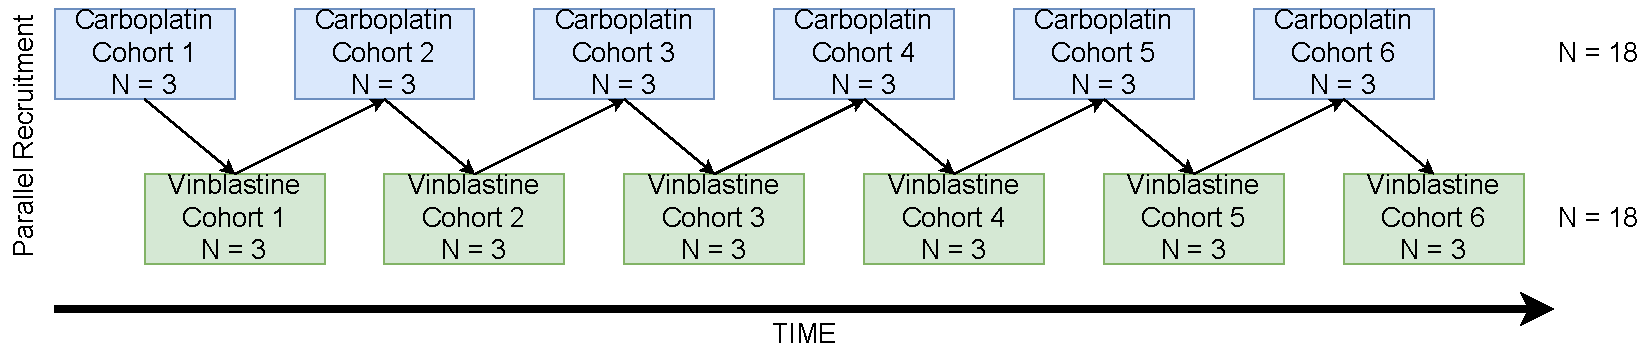
\includegraphics[width=\textwidth]{ETP-MonoGermFlipFlop}
\end{figure}

A Bayesian approach is implemented to assess the true CR rates. Specifically, the experimental monotherapies will need to demonstrate non-inferiority to the standard of care by a clinically acceptable margin. Based on previous data it was determined that the minimum CR rate with standard of care is 30\%. This value was taken as the non-inferiority margin. So, if the treatments have a CR rate $\geq30$\% they will be considered non-inferior. 

CR rates for each treatment arm will be established from the posterior probability distribution generated using a beta-binomial conjugate analysis. A minimally informative Beta(1,1) prior will be used in combination with the data observed during the trial to produce the posterior. In terms of decision making the following rule for the final analysis was specified: 

\begin{equation}
	P(CR \geq 30\%) \geq 0.8
\end{equation}

That is to say that if there is a high probability ($\geq 0.8$) that the true CR rate is $\geq30$\% there will be a GO decision, which in the context of this trial means the treatment arm would be deemed non-inferior. The minimum number of observed CRs out of the 18 patients needed to warrant a GO decision is seven. If seven responses are observed the median Bayesian estimate of the CR rate would be 40\% with a 0.82 probability that the true CR rate is $\geq30$\%. 

Stopping rules have also been implemented. At each interim analysis the predicted probability of success (PPoS) will be calculated. This is the probability that a GO decision would be made at the final analysis based on current data that has been accrued. Here the stopping rule is such that if the PPoS is less than 0.01 we would recommend stopping recruitment to that arm. 

It is important to note that whilst the trial has two arms it is not designed with the intention of making comparisons between the two treatments. Rather the trial aims to find if there is enough evidence that one of these treatments provides a sufficient response rate to warrant a GO decision.  

LK produced ETPs throughout the design of this trial. Figure \ref{fig_etp:MonoGermETP} shows the ETP for the design specified here. The ETPs produced here helped determine what data we wanted to present as well as how we structure the data in each of the cells. Here each cell shows the number of responses, the PPoS or the posterior probability that the response rate is $\geq30$\%, the Bayesian estimate of CR rate and a lower one-sided 80\% credible interval.

Calculations for these plots were conducted in STATA and the ETP was produced in Microsoft PowerPoint. One benefit of this approach is that the ETP can be easily customised and labelled. However, this meant that any changes in the design that affected the decision-making resulted in the ETP having to be updated manually. As a tool the ETP is effective at illustrating a final design but without the ability to easily generate them during the design of a trial they somewhat lose their purpose. This served as further motivation to produce some code or a tool that would allow for ETPs to be automatically created. 

\begin{sidewaysfigure}[h!]
	\centering
	\caption{ETP for the MonoGerm trial.}
	\label{fig_etp:MonoGermETP}
	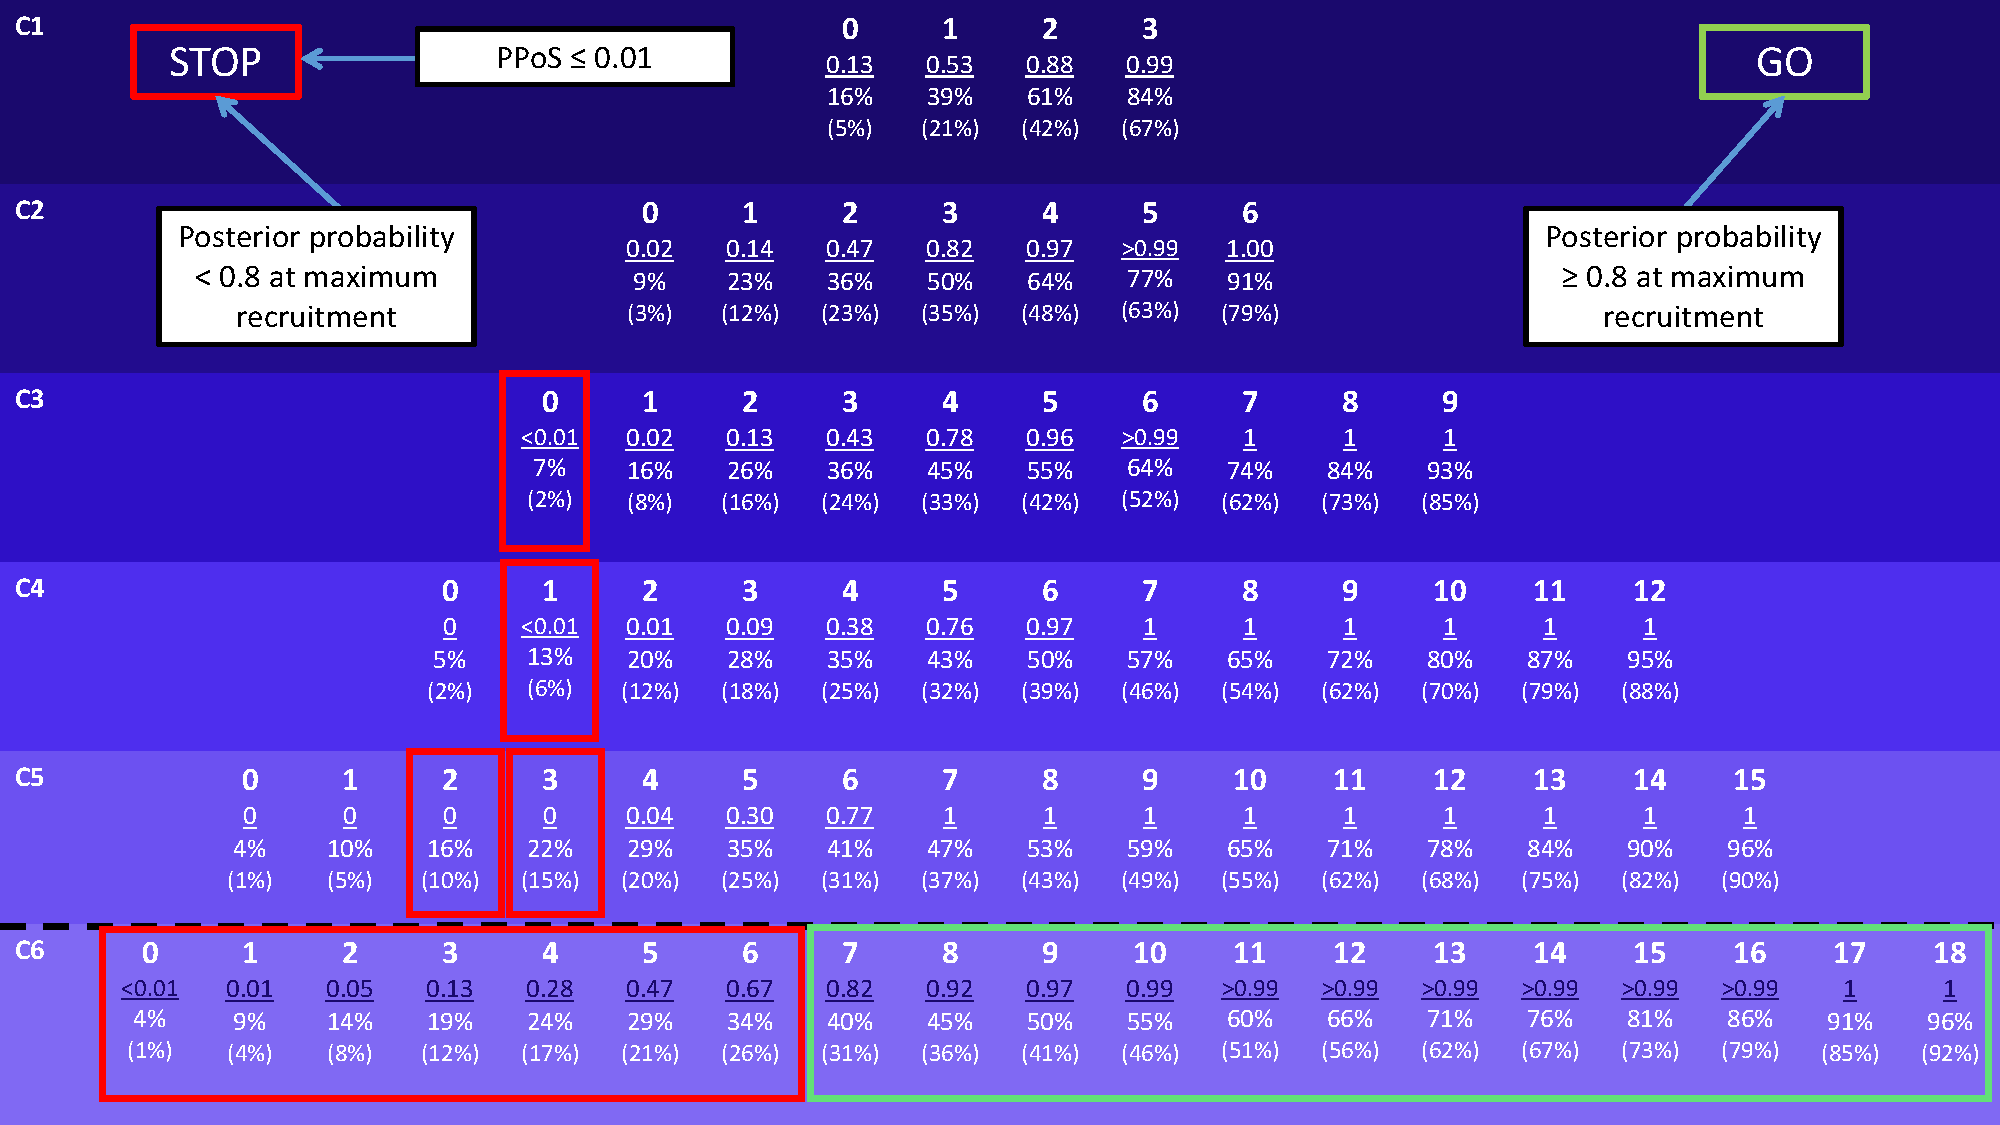
\includegraphics[width=23cm, height=15cm]{ETP-MonoGermETP}
\end{sidewaysfigure} 

\clearpage

%-----------------------------------
%	SUBSECTION 2
%-----------------------------------

\section{Glo-BNHL}

This trial was designed by Lucinda Billingham (LB) with the assistance of Shanna Maycock (SM). During initial stages of the design Grace Holt (GH) also assisted with the implementation of ETPs. This trial is currently still in set-up so specific details of the trial may be subject to change.   

The Glo-BNHL \footnote{A Global Study of Novel Agents in Paediatric and Adolescent Relapsed and Refractory B-cell Non-Hodgkin Lymphoma} study is a platform trial that aims to investigate the safety and effectiveness of novel treatments in children, adolescents and young adults with relapsed and/or refractory B-cell non-Hodgkin Lymphoma (r/r BNHL). This trial is an international collaboration and hopes to generate substantial evidence that could change practice in this rare cancer population. 

Inclusion of novel agents into the platform will be determined by an international Trial Steering Committee (TSC). Currently the platform consists of three separate treatment arms, each focusing on a different novel agent in a distinct group of patients. Each treatment arm will be treated independently which allows for them to be analysed separately. There may also be separate eligibility criteria for each arm. Patients will be enrolled into any arm where they are eligible. The three arms that will be available at the start of the trial are as follows: 

\begin{itemize}
	\item Treatment Arm \RN{1}: Bispecific Antibody (BsAb)
	\item Treatment Arm \RN{2}: Antibody-Drug Conjugate (ADC) with standard \\ chemotherapy
	\item Treatment Arm \RN{3}: Chimeric Antigen Receptor (CAR) T-cells
\end{itemize}

This trial utilises an adaptive Bayesian design, which enables GO/No GO decisions specific to the distinct populations in each treatment arm. The Bayesian approach has many benefits here as it facilitates decision making with small sample sizes. Decisions will be made based on the estimate of the probability that a novel agent is clinically effective. The specific criteria will vary between each treatment arm. This design and approach also allows for continuous evaluation of each novel agent. Treatment arms may be removed if the treatment is shown to be ineffective based on the trial data. Additionally, treatment arms may also be added or amended in the future if recommended by the TSC. 

Treatment arm \RN{1} aims to estimate the clinical efficacy of BsAb treatment in patients with r/r BNHL in first (only one prior line of therapy) or subsequent relapse (more than one prior line of therapy). Due to this treatment arm \RN{1} is split into two groups, \RN{1}a and \RN{1}b for patients with one relapse or more than one relapse respectively. These two subsequent arms will be recruited into and analysed separately. In terms of treatment these patients will receive odronextamab given as an intravenous infusion weekly for 12 weeks, then every two weeks until nine months, and every four weeks thereafter until progression or for a maximum of two years. The outcome measure for patients in treatment arms \RN{1}a and \RN{1}b is the occurrence of an objective response (OR) i.e. complete response (CR) or partial response (PR) after 12 weeks of treatment assessed by Independent Central Review. However, for interim analyses local response assessments will be used. 

Treatment arm \RN{2} aims to estimate the clinical efficacy of ADC treatment with modified R-ICE (rituximab, ifosphamide, carboplatin, etoposide and dexamethasone) chemotherapy in patients with r/r B-NHL in first or subsequent relapse. Patients will receive loncastuximab tesirine given as a 30 minute intravenous infusion with each cycle of modified R-ICE for a maximum of three cycles. Here the outcome measure is occurrence of CR within a maximum of three cycles of treatment. 

Treatment arm \RN{3} aims to estimate the efficacy of CAR T-cell therapy in r/r B-NHL patients who have CAR T-cell product available. The specific treatments patients will receive is yet to be defined. The outcome measure is the occurrence of OR following CAR T-cell infusion. 

Each treatment arm and subsequent treatment arm (i.e. \RN{1}a and \RN{1}b) will aim to recruit 15 evaluable patients during the initial stage. Once this recruitment is complete a transition analysis is performed leading to three possible outcomes. If the analysis results in a No GO decision recruitment to that treatment arm will stop. If the analysis result is a GO decision there are two options either there is sufficient evidence to change practice so the trial will stop recruiting or this will trigger an expansion stage in which a further 15 patients will be recruited. Following the expansion stage a confirmatory analysis will be conducted on all 30 evaluable patients. 

Interim analyses will be conducted after every three patients during the initial stage and after every five patients during the expansion stage. There will also be the option to stop recruitment to a treatment arm based on the data observed in the interim analysis. Figure \ref{fig_etp:Glo-BNHLflowchart} shows a flowchart of the decision making process for each arm in the trial. 

\begin{figure}[h!]
	\centering
	\caption{Flowchart of the decision making process in Glo-BNHL.}
	\label{fig_etp:Glo-BNHLflowchart}
	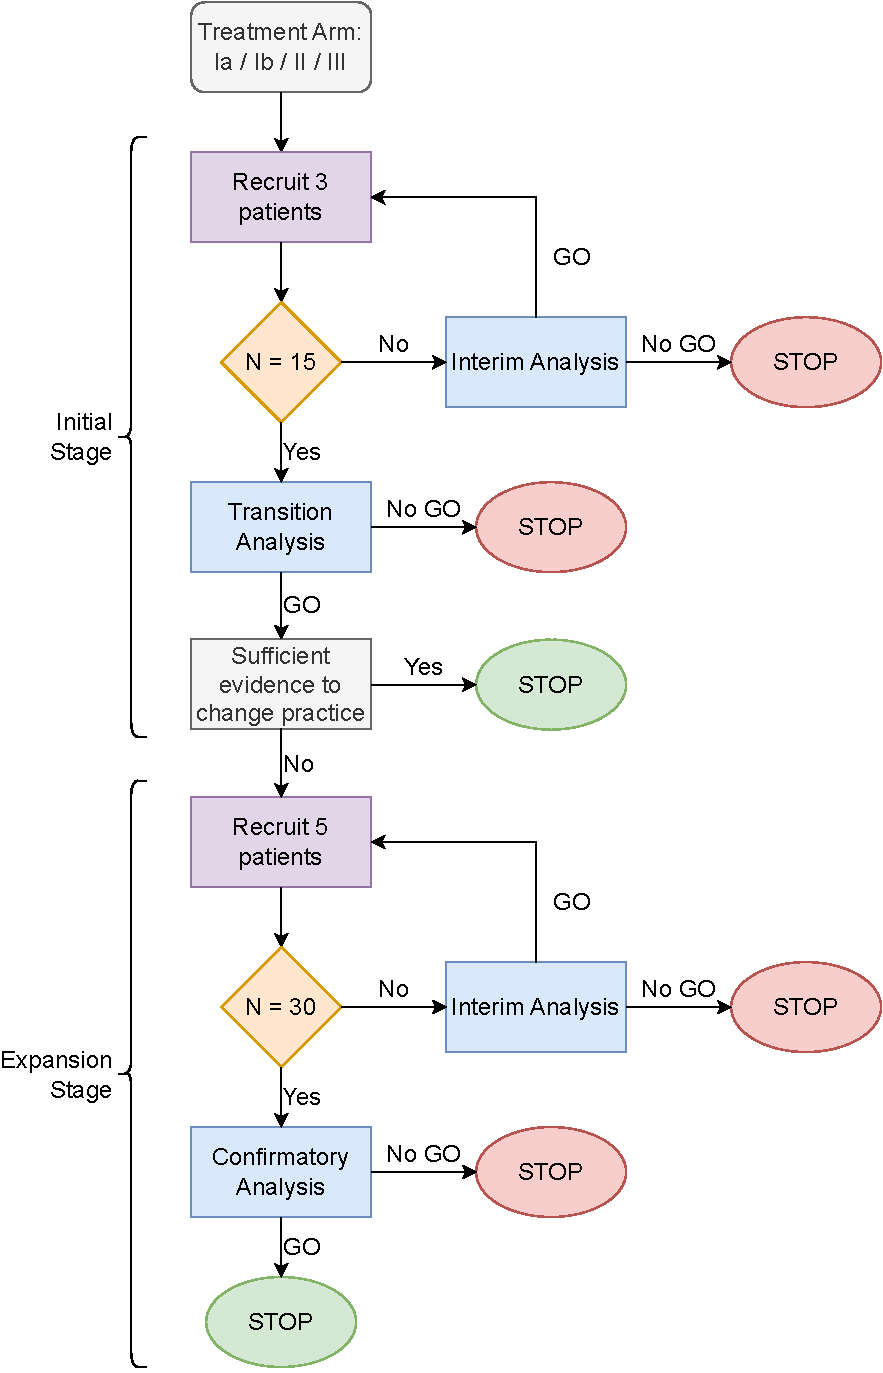
\includegraphics[width=0.9\textwidth]{ETP-GloBNHL-flowchart}
\end{figure}

A beta-binomial conjugate analysis will be conducted for each treatment arm. Observed trial data will be combined with a minimally informative Beta(1,1) prior to produce a posterior probability distribution for the treatment effect $\theta$, which represents either the OR/CR rate dependent on treatment arm. The posterior probability distribution is then used to inform decision making. GO/No Go decision criteria are specified separately for each treatment arm. 

For treatment arm \RN{1}a the decision criteria at the transition analysis is P($\theta$ > 40\%) $\geq$ 0.8. So, if the true OR rate was greater than 40\% with a probability of at least 0.8 based on the data collected in the trial there would be a GO decision. This corresponds to observing at least eight responses out of 15. For the confirmatory analysis a GO decision is made if P($\theta$ > 40\%) $\geq$ 0.95. At the final analysis we would need the probability that the true OR rate was greater than 40\% to be at least 0.95. Here a GO decision would only be made if 17 out of 30 patients had an OR. Table \ref{tab_etp:GloBNHL_decision_criteria} details the criteria for each treatment arm which can be interpreted in a similar manner. 

\begin{table}[h!]
	\centering
	\caption{Summary of decision criteria for Glo-BNHL.}
	\label{tab_etp:GloBNHL_decision_criteria}
	\resizebox{\textwidth}{!}{%
		\begin{tabular}{ccccc}
			\hline
			\multicolumn{1}{l}{\textbf{}} & \multicolumn{2}{c}{\textbf{Transition Analysis}}               & \multicolumn{2}{c}{\textbf{Confirmatory Analysis}}             \\ \cline{2-5} 
			\textbf{Treatment Arm}        & \textbf{Decision Criteria} & \textbf{Min No. Responses for GO} & \textbf{Decision Criteria} & \textbf{Min No. Responses for GO} \\ \hline
			Ia  & P($\theta$ \textgreater 40\%) $\geq$ 0.8 & 8/15 & P($\theta$ \textgreater 40\%) $\geq$ 0.95 & 17/30 \\
			Ib  & P($\theta$ \textgreater 10\%) $\geq$ 0.8 & 3/15 & P($\theta$ \textgreater 10\%) $\geq$ 0.95 & 6/30  \\
			II  & P($\theta$ \textgreater 20\%) $\geq$ 0.8 & 5/15 & P($\theta$ \textgreater 20\%) $\geq$ 0.95 & 10/30 \\
			III & P($\theta$ \textgreater 10\%) $\geq$ 0.8 & 3/15 & P($\theta$ \textgreater 10\%) $\geq$ 0.95 & 6/30  \\ \hline
		\end{tabular}%
	}
\end{table}

For the interim analyses there are separate stopping rules. These are the same across the treatment arms but differ in the initial stage compared to the expansion stage. During the initial stage, the predicted probability of success at the transition analysis (PPoSt) is calculated and decisions are made based on the following criteria: 

\begin{enumerate}
	\item PPoSt < 0.01 - recommend stopping for futility
	\item 0.01 $\leq$ PPoSt < 0.05 - consider stopping for futility
	\item 0.05 $\leq$ PPoSt < 0.15 - consider whether sufficient benefit in continuing 
	\item PPoSt $\geq$ 0.15 - recommend continuing 
\end{enumerate}

So, if the probability of success at the transition analysis is less than 1\% the recommendation would be to stop recruitment to the treatment arm and if it was greater than or equal to 15\% the recommendation would be to continue recruitment. If PPoSt is between 1-5\% or 5-15\% stopping should be also be considered for either futility or if there sufficient benefit in continuing respectively.  

At the expansion stage, the predicted probability of success at the confirmatory analysis is used (PPoSc). If this is below 10\% (PPoSc < 0.1) the recommendation would be to stop recruitment to that treatment arm due to futility. It should be noted that these decision rules are only recommendations and the independent data monitoring committee (DMC) will make decisions based on not only primary outcomes but secondary outcomes, recruitment and safety data. 

For this trial ETPs were produced separately for each treatment arm and for each stage. This resulted in eight ETPs, one for the initial stage showing the outcome of the transition analysis and one for the expansion stage showing the outcome of the confirmatory analysis for each treatment arm (\RN{1}a, \RN{1}b, \RN{2}, \RN{3}). ETPs were utilised throughout the design of the trial with initial versions originally created by GH using STATA and Microsoft PowerPoint. These were then further developed by SM who performed calculations in R but still utilised PowerPoint to create the ETPs. Figure \ref{fig_etp:GloBNHL-ETP-TA1aInitial} and \ref{fig_etp:GloBNHL-ETP-TA1aExtenstion} shows the ETPs for the initial and expansion stage of treatment arm \RN{1}a respectively. These ETPs created by SM helped us determine how our function and app visually presented ETPs and we utilised a similar colour scheme. 

Similar to MonoGerm the process of creating these ETPs in PowerPoint can be time consuming. This is even more of an issue in the Glo-BNHL study due to the multiple treatment arms and stages. Additionally, this trial highlighted another issue when you have multiple statisticians working on a trial who use different software packages. In this case it would mean work would have to be recreated in R and STATA to conduct the calculations required for ETPs. This served as further motivation for the development of an application which requires no specific stats software knowledge. As statisticians would easily be able to recreate ETPs. SM went on to further extend the function we developed to automatically generate ETPs specific to Glo-BNHL. 

\begin{sidewaysfigure}[h!]
	\centering
	\caption{ETP for the initial stage of treatment arm \RN{1}a in Glo-BNHL.}
	\label{fig_etp:GloBNHL-ETP-TA1aInitial}
	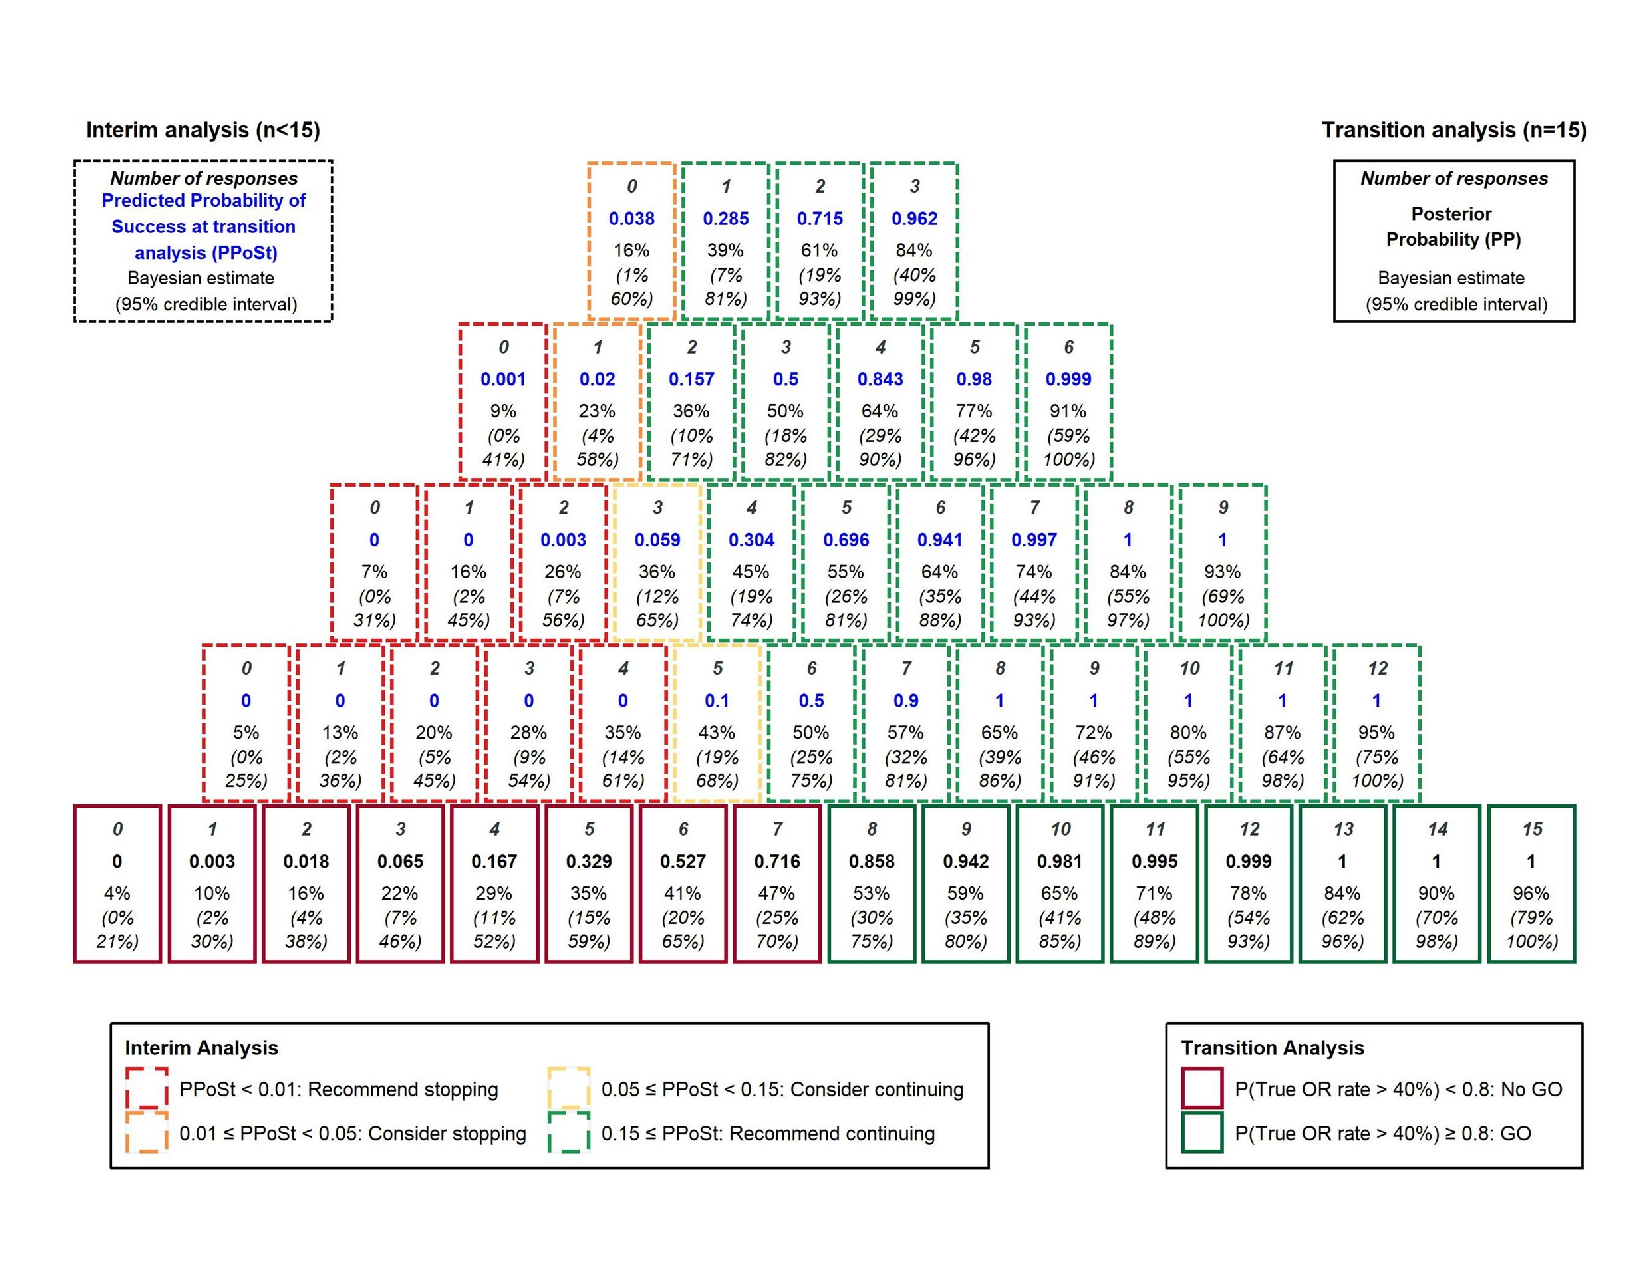
\includegraphics[width=23cm, height=15cm]{ETP-GloBNHL-ETP-TA1aInitial}
\end{sidewaysfigure} 

\begin{sidewaysfigure}[h!]
	\centering
	\caption{ETP for the expansion stage of treatment arm \RN{1}a in Glo-BNHL.}
	\label{fig_etp:GloBNHL-ETP-TA1aExtenstion}
	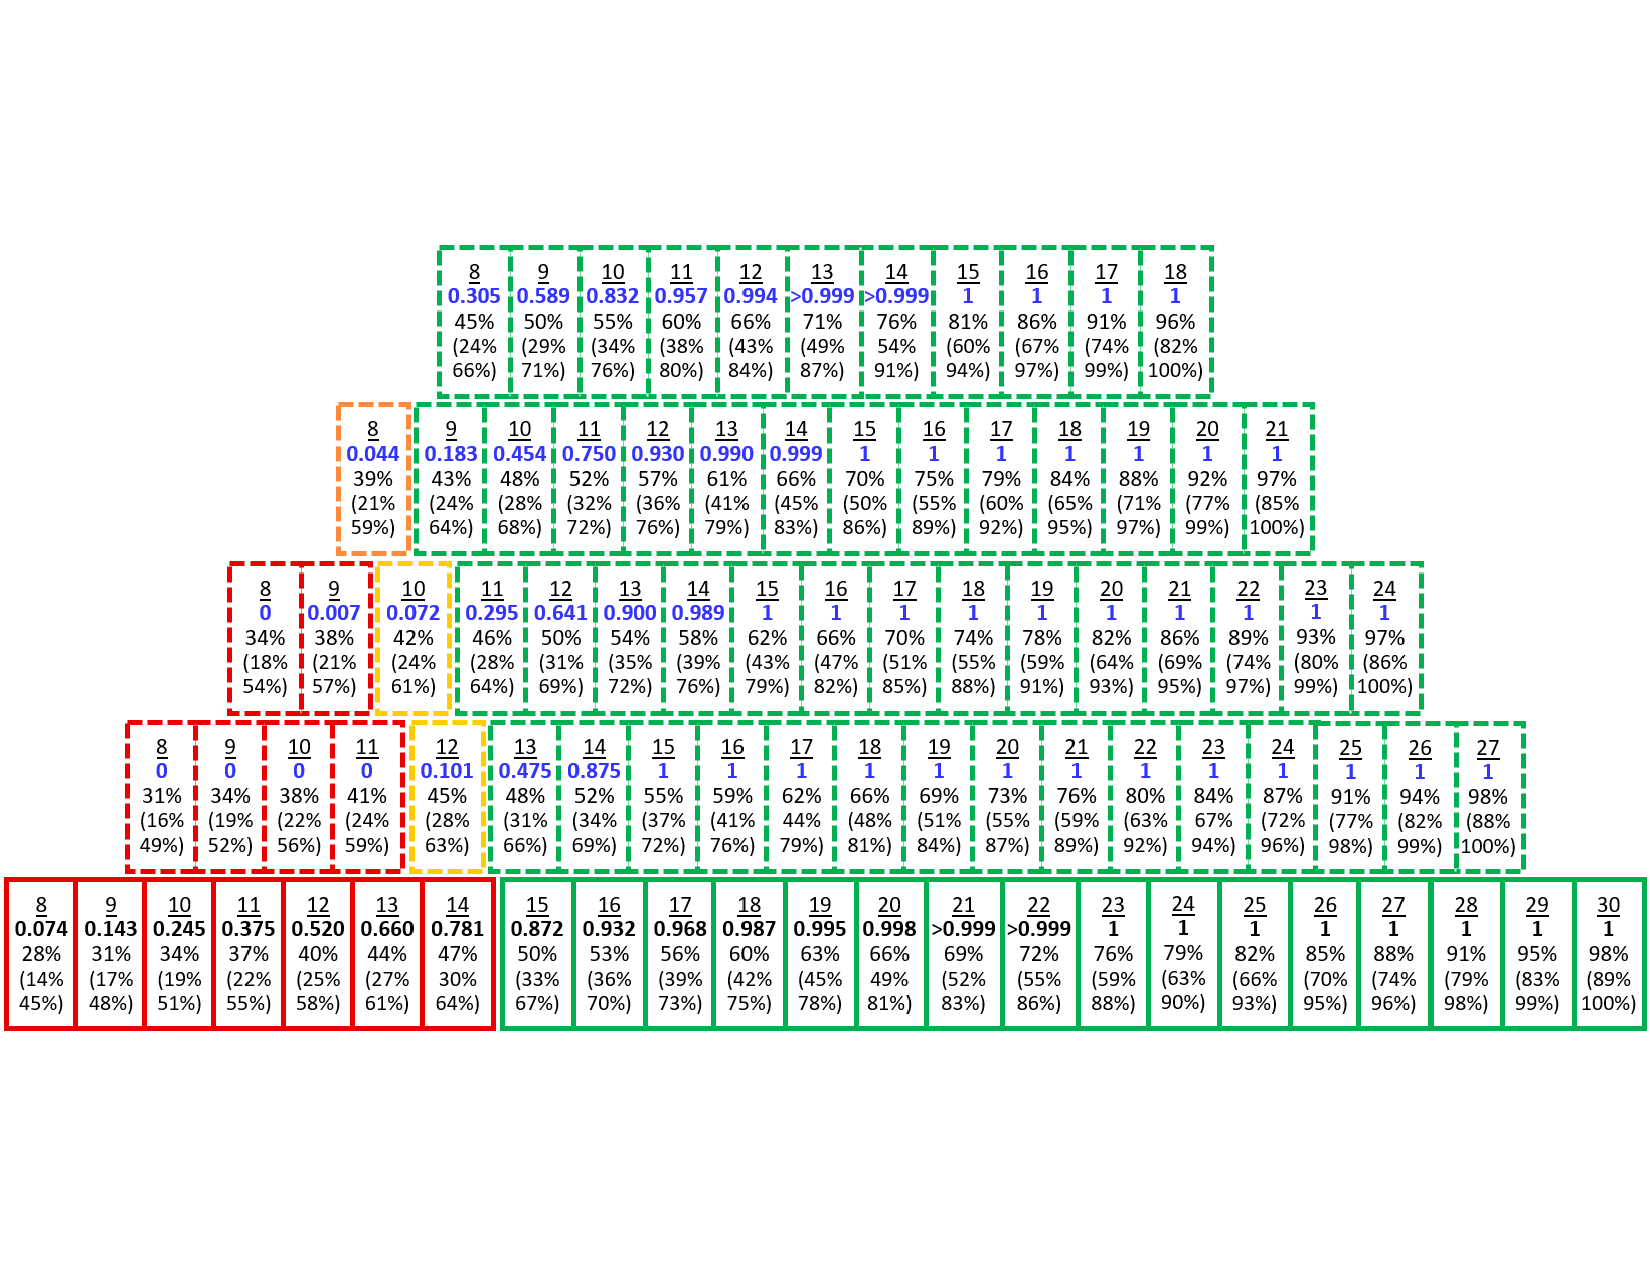
\includegraphics[width=23cm, height=15cm]{ETP-GloBNHL-ETP-TA1aExtension}
\end{sidewaysfigure} 

\clearpage

%-----------------------------------
%	SUBSECTION 3
%-----------------------------------

\section{DETERMINE}

DETERMINE \footnote{Determining Extended Therapeutic indications for Existing drugs in Rare Molecularly-defined Indications using a National Evaluation platform trial} is a trial that was also designed by Lucinda Billingham (LB). It is an umbrella-basket platform trial with multiple treatment arms running in parallel. The trial aims to evaluate the efficacy of targeted therapies in rare cancers with actionable genomic alterations, including common cancers with rare actionable alterations. This trial is currently open to recruitment and may be expanded in the future as more drugs are bought onto the platform.  

DETERMINE will recruit patients of all ages including, paediatric, TYA (teenage and young adult) and adults, who have rare tumours that contain an actionable genetic alteration that can be targeted therapeutically. The genetic alteration must have been identified previously from a tissue biopsy or ctDNA (circulating tumour DNA). Patients will then be stratified into molecular groups based on their tumour profile and allocated to the most suitable treatment arm by the Molecular Tumour Board (MTB). The umbrella part of the design consists of multiple non-randomised treatment arms, each evaluation a licensed targeted anti-cancer drug or drug combination in a specific molecularly-defined group of patients. Each molecularly-defined group allocated to a specific treatment arm will contain multiple baskets of different tumour types, age groups and molecular subtypes. This is visualised in Figure \ref{fig_etp:DETERMINEDesign}. 

\begin{figure}[h!]
	\centering
	\caption{Umbrella-basket platform trial design in DETERMINE.}
	\label{fig_etp:DETERMINEDesign}
	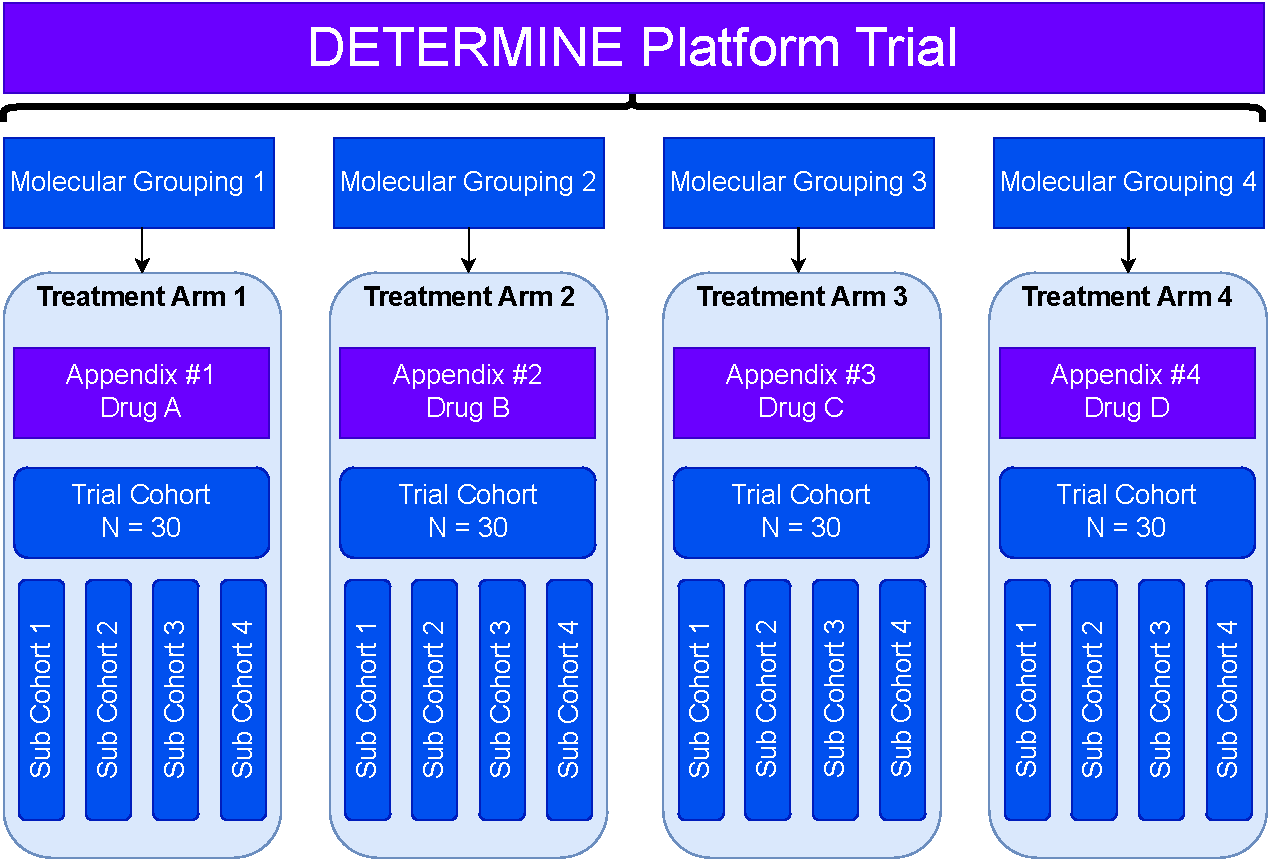
\includegraphics[width=\textwidth]{ETP-DETERMINEDesign}
\end{figure}

A main trial cohort of 30 evaluable patients will be recruited into each treatment arm. This will include patients with different tumour types, ages and molecular subtypes. If specific subgroups within this main cohort are experiencing significant benefit from treatment sub-cohorts will be formed to investigate treatment effectiveness in these subgroups. It is possible for each treatment arm to have multiple sub-cohorts and they can recruit in parallel to the main cohort. Each sub-cohort will be subject to the same statistical analysis and will also aim to recruit 30 patients. Currently there are five treatment arms, details of these are provided in Table \ref{tab_etp:DETERMINE_trtarms}. 

\begin{table}[h!]
	\fontsize{10pt}{10pt}\selectfont
	\centering
	\caption{Current treatment arms in DETERMINE}
	\label{tab_etp:DETERMINE_trtarms}
	\resizebox{\textwidth}{!}{%
		\begin{tabular}{p{0.1\textwidth} | p{0.2\textwidth} | p{0.5\textwidth} | p{0.2\textwidth}}
			Treatment Arm  & IMP(s) & Molecular Grouping & Route and Formulation \\ \hline
			1 &  Alectinib & ALK gene fusion positive solid tumours & Oral capsules \\ \hline
			2 & Atezolizumab & Solid tumours with high tumour mutational burden (TMB) or microsatellite instability-high (MSI-high) or proven constitutional mismatch repair deficiency (CMMRD) disposition & Intravenous (IV) infusion  \\ \hline
			3 & Entrectinib & NTRK or ROS1 gene fusion positive solid tumours & Oral capsules; Dosing depends on body surface area (BSA) \\ \hline
			4 & Trastuzumab in combination with pertuzumab & Solid tumours with HER2 amplification or mutations & IV infusion \\ \hline 
			5 & Vemurafenib in combination with cobimetinib & Solid tumours with BRAF V600 mutations & Oral; 960 mg tablets \\ \hline
		\end{tabular}
	}
\end{table}

Co-primary outcomes of objective response (OR) and durable clinical benefit (DCB) will be used to assess efficacy of the treatment in each of the cohorts in each molecular grouping. These are both classified as binary variables. OR is defined dependent on specific disease criteria. DCB is defined as the absence of disease progression for at least 24 weeks from the start of trial treatment, this will also be measured based on disease specific criteria. Patients will receive treatment based on the license schedule for the drug in their treatment arm. Patients continue treatment until either they reach progressive disease (PD), unacceptable adverse events or withdraw from the trial. 

All outcomes in each treatment arm, cohort and sub cohort will be analysed using a Beta-Binomial conjugate analysis. Posterior probability distributions for OR and DCB will be generated using minimally informative priors, Beta(0.1,0.9) and data that is collected on the trial. However decision making will be done using the BOP-2 design \cite{zhouBOP2BayesianOptimal2017,zhouBayesianOptimalPhase2020}. This design makes GO or No GO decisions by assessing posterior probabilities for a set of outcomes, which are optimised to either maximise power or minimise the number of patients. The design also allows for the control of type I and type II error rates. In DETERMINE, for each co-primary outcome, a rate of 10\% or less would represent a treatment effect that is not clinically relevant and a rate of 30\% would represent a clinically meaningful treatment effect. These can be thought of as a null and alternative hypothesis. The use of this design was made possible due to the development of web applications by the authors at the MD Anderson Cancer Centre \cite{tidwellBayesianClinicalTrials2019}. 

Interim analyses will be conducted throughout the trial, however formal decision making will first be conducted after 10 evaluable patients have been recruited and then every 5 patients from that time-point in each cohort/sub-cohort. If probability that both the true OR and DCB rates are lower than the critical threshold of 10\% the trial would recommend stopping. The design is optimised to minimise the type II error i.e. to minimise the probability of not rejecting the null hypothesis when treatment is effective. This is done whilst controlling the type I error rate at 0.1. Under the BOP-2 design this provides the following stopping boundaries of 0/10, $\leq$1/15, $\leq$2/20, $\leq$3/25 at each of the planned analyses at 10, 15, 20 and 25 patients. For the final analysis at 30 patients there would be a GO decision if $\geq$6/30 patients had either a OR or DCB.   

The ETPs we have shown so far all have been based on a Beta-Binomial conjugate analysis with decisions made using PPoS and the posterior distribution. However, they can also be utilised here. LB created the ETP shown in Figure \ref{fig_etp:DETERMINE-ETP}. Here we can see each cell still pertains to a specific number of responses out of a certain number of patients. Bayesian estimates, credible intervals and posterior probabilities of the treatment effect being greater than our null and alternative hypothesis. The cells have then been colour coded based on the decision criteria elicited from the BOP-2 design. This trial also shows that ETPs are a flexible tool that can also be applied to trials not explicitly using a Beta-Binomial conjugate analysis for decision making. 

\begin{sidewaysfigure}[h!]
	\centering
	\caption{ETP for the DETERMINE trial.}
	\label{fig_etp:DETERMINE-ETP}
	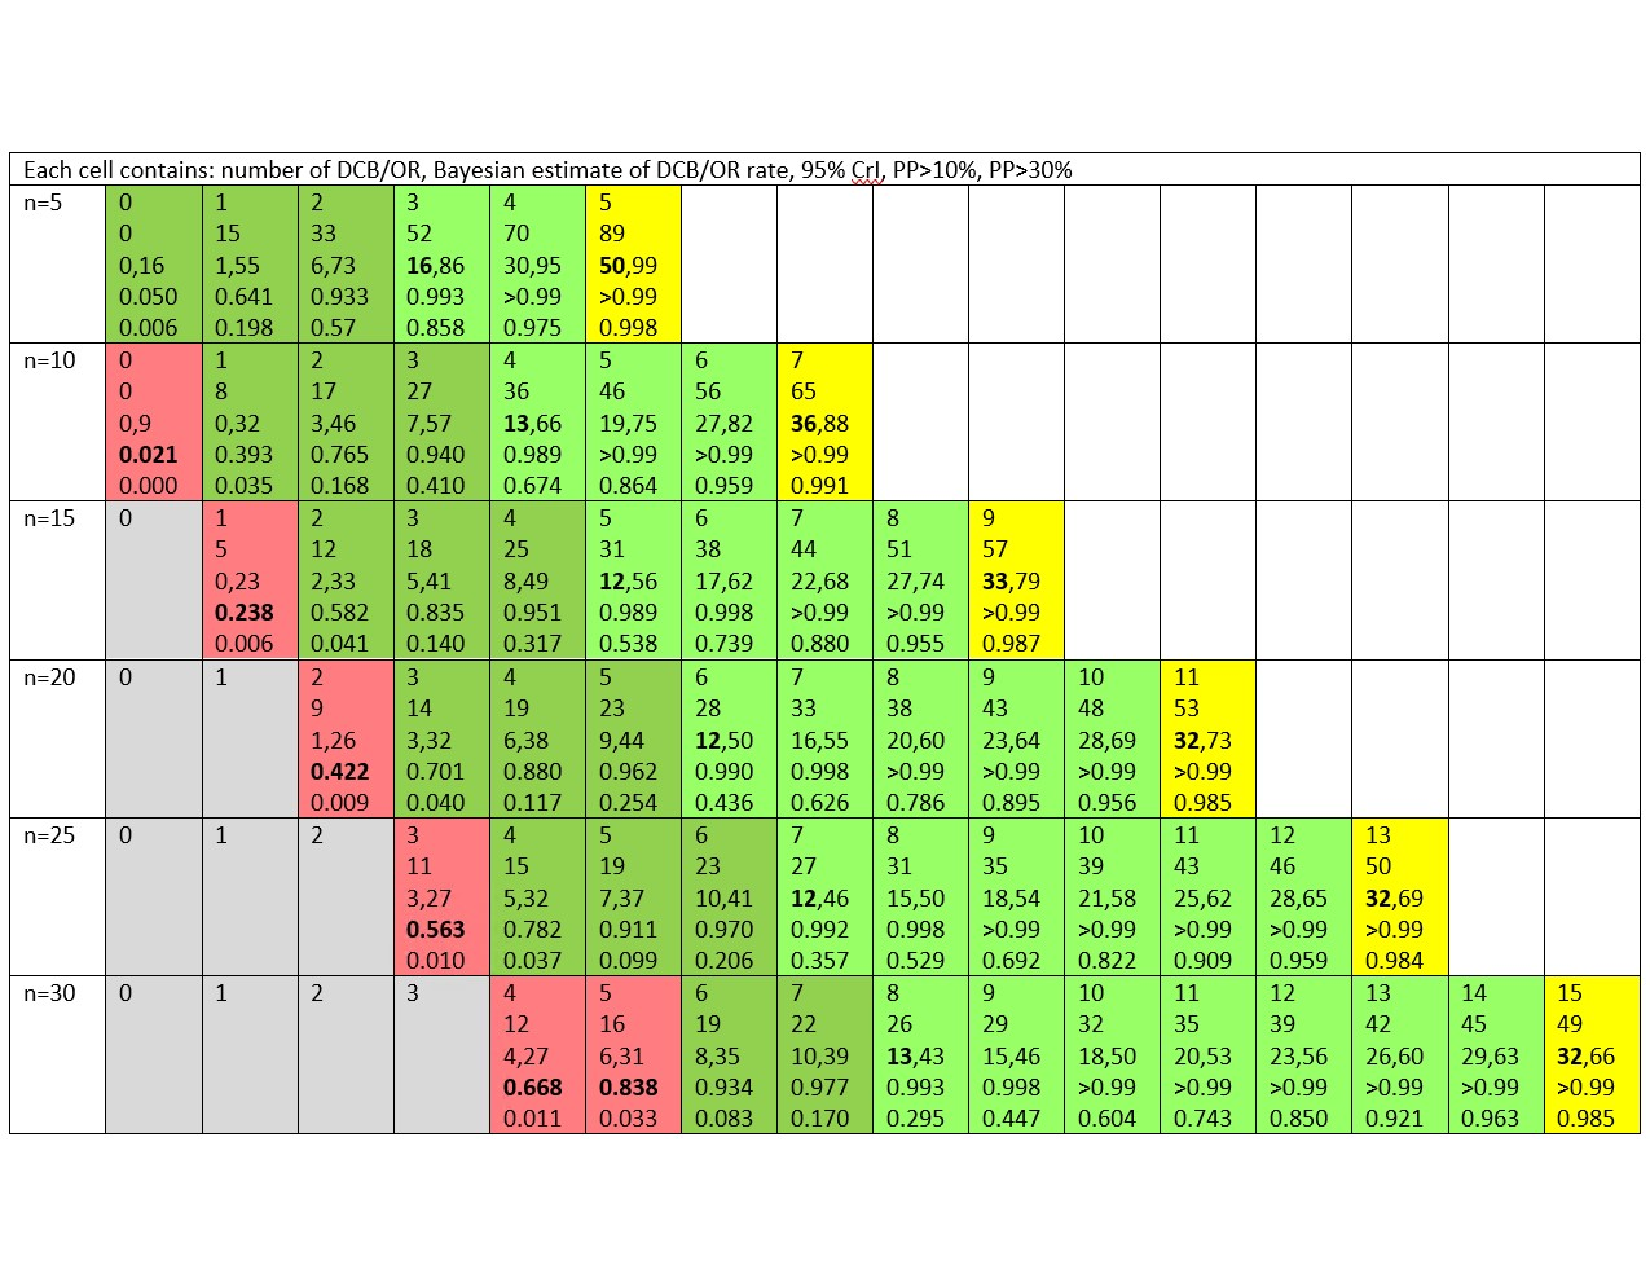
\includegraphics[width=23cm, height=15cm]{ETP-DETERMINE-ETP}
\end{sidewaysfigure} 

\clearpage
%\include{Appendices/AppendixB}
%\include{Appendices/AppendixC}

%----------------------------------------------------------------------------------------
%	BIBLIOGRAPHY
%----------------------------------------------------------------------------------------

\printbibliography[heading=bibintoc]

%----------------------------------------------------------------------------------------

\end{document}  
